\input{chap/myDefbook.tex}
\title{baby-rudin reading notes}
\author{weiyuan}
\date{\today}

\begin{document}
\frontmatter
\maketitle
\tableofcontents
\mainmatter
% chap00
\chapter*{Preface}
\label{chap:00}
This book is intended to serve as a text for the course in analysis that is usually
taken by advanced undergraduates or by first-year students who study mathematics.


The present edition covers essentially the same topics as the second one,
with some additions, a few minor omissions, and considerable rearrangement.
I hope that these changes will make the material more accessible amd more attractive to the students who take such a course.


Experience has convinced me that it is pedagogically unsound (though
logically correct) to start off with the construction of the real numbers from the
rational ones.
At the beginning, most students simply fail to appreciate the need
for doing this.
Accordingly, the real number system is introduced as an ordered
field with the least-upper-bound property, and a few interesting applications of
this property are quickly made.
However, Dedekind's construction is not omitted.
It is now in an Appendix to Chapter I, where it may be studied and enjoyed
whenever the time seems ripe.


The material on functions of several variables is almost completely rewritten, with many details filled in, and with more examples and more motivation.
The proof of the inverse function theorem---the key item in Chapter \ref{chap:09}---is
simplified by means of the fixed point theorem about contraction mappings.

Differential forms are discussed in much greater detail.
Several applications of
Stokes' theorem are included.


As regards other changes, the chapter on the Riemann-Stieltjes integral
has been trimmed a bit, a short do-it-yourself section on the gamma function
has been added to Chapter \ref{chap:08}, and there is a large number of new exercises, most
of them with fairly detailed hints.


I have also included several references to articles appearing in the \emph{American Mathematical Monthly} and in \emph{Mathematics Magazine}, in the hope that students
will develop the habit of looking into the journal literature.
Most of these
references were kindly supplied by R. B. Burckel.


Over the years, many people, students as well as teachers, have sent me
corrections, criticisms, and other comments concerning the previous editions
of this book.
I have appreciated these, and I take this opportunity to express my sincere thanks to all who have written me.



WALTER RUDIN

% chap01
\chapter{The real and complex number system}
\label{chap:01}
\section{Introduction}
First we use $\sqrt{2}$ to construct real number system from integer and rational numbers.

\begin{newexample}
    \label{newexample:1.1}
    \begin{equation}
        \label{eq:1.1}
        p^2=2
    \end{equation}
    $p$ is not a rational number.
\end{newexample}

\begin{proof}
    If $p$ is rational,  $\exists m,n \in \mathbf{N}$,
    s.t. $p=m/n$. $\gcd (m,n) = 1$.
    Then \ref{eq:1.1}
    \begin{equation}
        \label{eq:1.2}
        m^2 = 2n^2.
    \end{equation}

    $m$ is even, $m = 2k$.
    Then $(2k)^2 = 2n^2$, $2k^2 = n^2$, $k$ is even, $\gcd (m,n)=2\neq 1$,
    contrary to our choice of $m$ and $n$. Hence p can't be a rational number.
\end{proof}

After proving $\sqrt{2}$ isn't a rational number, rudin use $\sqrt{2}$ to divide the rationals

\mybox{
    在证明 $\sqrt{2}$ 不是有理数后,
    使用 $\sqrt{2}$ 将有理数集分成两部分.
    引出了分划的概念?
}

\begin{align*}
    A = \{p|p^2<2\} \\
    B = \{p|p^2>2\}
\end{align*}
$A$ \emph{contains no largest number},\\
$B$ \emph{contains no smallest number}.\\
$\forall p\in A$, $\exists q\in A$, s.t. $p<q$,\\
$\forall p\in B$, $\exists q\in B$, s.t. $p>q$,\\
$\forall p>0$
\begin{equation}
    \label{eq:1.3}
    q = p-\frac{p^2-2}{p+2} = \frac{2p+2}{p+2}
\end{equation}

Then
\begin{equation}
    \label{eq:1.4}
    q^2 - 2 = \frac{2(p^2-2)}{(p+2)^2}
\end{equation}

If $p\in A$, $p^2<2$. \ref{eq:1.3} shows that $q>p$, \ref{eq:1.4} shows that $q^2<2$, $q\in A$.

If $p\in B$, $p^2>2$. \ref{eq:1.3} shows that $q<p$, \ref{eq:1.4} shows that $q^2>2$, $q\in B$.


\begin{myremark}
    \label{myremark:1.2}
    The purpose of the above discussion has been to show that
    the rational number system has \myKeywordred{certain gaps},
    in spite of the fact that between any two rationals there is another:
    If $r<s$ then $r<(r+s)/2<s$.
    The real number system fills these gaps.
    This is the principal reason for the fundamental role
    which it plays in analysis.
\end{myremark}

\mybox{
    有理数的稠密性与实数的连续性.
    在分析中, 考察极限等需要的是数系的连续性, 因此需要先建立实数系.
    事实上, 我们是先有微积分, 后有实数理论的. \\
    三次数学危机:无理数, 微积分基础, 集合论
    实数理论是极限的基础.
}

In order to elucidate its structure, as well as that of the complex numbers,
we start with a brief discussion of the general concepts of \myKeywordblue{ordered set} and \myKeywordblue{field}.

% \mybox{
%     rudin引入复数的方法非常怪, 对初学者非常不友好, 过于抽象了. 
%     % 想起一个法国笑话, 问小学生$2+3$等于几, 回答 $2+3=3+2$ 加法是一个交换群(Abel 群)...
% } 

Here is some of the standard set-theoretic terminology that will be used throughout this book.

% \mybox{接下来引入一些集合论的概念}

\mybox{这里未经定义就使用了集合 Set 的概念

    Set  \url{https://mathworld.wolfram.com/Set.html}

    A set is a finite or infinite collection of objects
    in which order has no significance,
    and multiplicity is generally also ignored
    (unlike a list or multiset).
    Members of a set are often referred to as elements
    and the notation $a \in A$ is used to denote that
    $a$ is an element of a set $A$.
    The study of sets and their properties is the object of set theory.

    % Older words for set include aggregate and set class. 
    % Russell also uses the unfortunate term manifold to refer to a set.

    % Historically, 
    % a single horizontal overbar was used to denote 
    % a set stripped of any structure besides order, 
    % and hence to represent the order type of the set. 
    % A double overbar indicated stripping the order from the set 
    % and hence represented the cardinal number of the set. 
    % This practice was begun by set theory founder Georg Cantor.

    % Symbols used to operate on sets include 
    % intersection $\cap$ (which means "and" or intersection), 
    % and union $\cup$ (which means "or" or union). 
    % The symbol emptyset $\varnothing$ is used to denote 
    % the set containing no elements, called the empty set.

    % There are a number of different notations related to the theory of sets. 
    % In the case of a finite set of elements,
    % one often writes the collection inside curly braces, e.g.,
    % \[A={1,2,3}\]
}

%  too long notes out side box

% for the set of natural numbers less than or equal to three. Similar notation can be used for infinite sets provided that ellipses are used to signify infiniteness, e.g.,
% \[B={3,4,5,...} 	\]

% for the collection of natural numbers greater than or equal to three, or
% \[C={...,-4,-2,0,2,4,...} 	\]

% for the set of all even numbers.

% In addition to the above notation, one can use so-called set builder notation to express sets and elements thereof. The general format for set builder notation is
% \[{x:p(x)}, 	\]

% where $x$ denotes an element and $p(x)$ denotes a property $p$ satisfied by $x$. $()$ can also be expanded so as to indicate construction of a set which is a subset of some ambient set $X$, e.g.,
% \[{x \in X:p(x)}. 	\]



% It is worth noting is that the "$:$" in $()$ and $()$ is sometimes replaced by a vertical line, e.g.,
% \[{x \in X|p(x)}. 	\]
% Also worth noting is that the sets in $()$, $()$, and $()$ can all be rewritten in set builder notation as subsets of the set Z of integers, namely
% \begin{align*}
%     A	&=	{n \in N:n<=3}	\\
%     B	&=	{n \in N:n>=3}	\\
%     C	&=	{n \in Z:n\text{ is even}},	
% \end{align*}
% respectively.

% \mybox{

% Other common notations related to set theory include $A^B$, which is used to denote the set of maps from $B$ to $A$ where $A$ and $B$ are arbitrary sets. 
% For example, an element of $X^\N$ would be a map from the natural numbers $\N$ to the set $X$. 
% Call such a function $f$, then $f(1)$, $f(2)$, etc., are elements of $X$, so call them $x_1, x_2$, etc. This now looks like a sequence of elements of $X$, so sequences are really just functions from $\N$ to $X$. This notation is standard in mathematics and is frequently used in symbolic dynamics to denote sequence spaces.

% Let $E, F$, and $G$ be sets. Then operation on these sets using the intersection and union operators is commutative
% \begin{align*}
%     E \cap F &= F \cap E \\	
%     E \cup F &= F \cup E, 	
% \end{align*}

% associative
% \begin{align*}
%     (E \cap F) \cap G &= E \cap (F \cap G) 	\\
%     (E \cup F) \cup G &= E \cup (F \cup G), 	
% \end{align*}

% and distributive
% \begin{align*}
%     (E \cap F) \cup G &= (E \cup G) \cap (F \cup G) 	\\
%     (E \cup F) \cap G &= (E \cap G) \cup (F \cap G). 	
% \end{align*}

% More generally, we have the infinite distributive laws
% \begin{align*}
%     A \cap ( \bigcup_{(\lambda \in \Lambda)}B_\lambda) &= \bigcup_{(\lambda \in \Lambda)}(A \cap B_\lambda) 	\\
%     A \cup ( \bigcap_{(\lambda \in \Lambda)}B_\lambda) &= \bigcap_{(\lambda \in \Lambda)}(A \cup B_\lambda) 	
% \end{align*}

% where lambda runs through any index set $\Lambda$. The proofs follow trivially from the definitions of union and intersection.
% }

\begin{mydef}
    \label{mydef:1.3}
    If $A$ is any set (whose elements may be numbers or any other objects),
    we write $x\in A$ to indicate that $x$ is a member (or an element) of $A$.
    \mybox{
        element 还没定义\\
        object指代什么? 我个人认为集合理解的难点在于集合的集合.
        % 这一点可以引出罗素悖论
    }
    If $x$ is not a member of $A$, we write: $x\notin A$.

    \emph{empty set} $\varnothing$ contains no element, If a set has at least one element, it is called \emph{nonempty}.

    $A,B$ are sets,
    $\forall x\in A$, $x\in B$, we say that $A$ is a \emph{subset} of $B$, $A \subset B$ or $B \supset A$.
    If $\exists x\in B$, $x\notin A$, A is a \emph{proper subset} of $B$, $A \subsetneqq B$.
    Note that $A\subset A$ for every set $A$.

    (Bernstein) If $A\subset B$ and $B\subset A$, we write $A = B$. Otherwise $A \neq B$.
\end{mydef}
\mybox{这条性质在证明集合相等时很常用}

\begin{mydef}
    \label{mydef:1.4}
    Throughout Chap. \ref{chap:01}, the set of all rational numbers will be denoted by $\Q $.
\end{mydef}
\section{Ordered sets}
\mybox{有序集}

\begin{mydef}\label{mydef:1.5}
    Let $S$ be a set. 
    An \myKeywordblue{order} on $S$ is a relation, denoted by $<$,
    with the following two properties:
    \begin{asparaenum}[(i)]
        \item If $x\in S$ and $y\in S$ then one and only one of the statements
        \begin{equation*}
            x<y, \quad
            x=y, \quad
            y<x
        \end{equation*}
        is true.    
        \item If $x,y,z\in S$, if $x<y$ and $y<z$, then $x<z$.
    \end{asparaenum}

    The statement $x < y$ may be read as 
    $x$ is less than $y$, or 
    $x$ is smaller than $y$, or
    $x$ precedes $y$.
    (It's often convenient to write $y>x$ in place of $x<y$)
    (less-great, smaller-bigger, precedes-succeeds)

    \mybox{form wiki,\\
    The relationship x precedes y is written $x ≺ y$.  \\
    The relation x precedes or is equal to y is written x ≼ y. \\
    The relationship x succeeds (or follows) y is written x ≻ y.  \\
    The relation x succeeds or is equal to y is written x ≽ y. \\
    ≺ $\backslash\text{prec}$  \\
    ≼ $\backslash\text{preccurlyeq}$  \\
    ≻ $\backslash\text{succ}$  \\
    ≽ $\backslash\text{succcurlyeq}$  } 

    $x\leq y$ indicates that $x<y$ or $x=y$, 
    without specifying which of these two is to hold.
    In other words, $x\leq y$ is the negation of $x>y$.
\end{mydef}


\mybox{
  偏序关系:
1. 三歧性,
2. 传递性.

建立偏序关系后, 可以使用不等式进行分析. 
在后续根据极限定义计算时, 
需要大量使用不等式分析数列和函数的极限计算结果. }

\begin{mydef}
    \label{mydef:1.6}
An \myKeywordblue{ordered set} is a set $S$ in which an order is defined.
\end{mydef}

For Example, $\Q $ is an ordered set 
if $r<s$ is defined to mean that $s-r$ is a positive rational number.

\mybox{
    存在偏序关系的集合称为有序集
$\Q , \R$ 均是有序集, 但$\mathbb{C}$ 不是有序集. }

\begin{mydef}
    \label{mydef:1.7}
    (bounded above)\\
    Suppose $S$ is an ordered set, and $E \subset S$. 
    If there exists a $\beta \in S$ 
    such that $x \leq \beta$ for every $x \in E$, 
    we say that $E$ is \myKeywordblue{bounded above}, and call
    $\beta$ an \myKeywordblue{upper bound} of $E$.

    Lower bounds are defined in the same way (with $\geq$ in place of $\leq$).
\end{mydef}

\begin{mydef}
    \label{mydef:1.8}
    (least upper bound)\\
    Suppose $S$ is an ordered set, $E \subset S$, and $E$ is bounded above.
    Suppose there exists an $a\alpha \in S$ with the following properties:
    \begin{enumerate}[(i)]
        \item $\alpha$ is an upper bound of $E$.
        \item If $\gamma <\alpha$ then $\gamma$ is not an upper bound of $E$.
    \end{enumerate}

    Then $\alpha$ is called the \myKeywordblue{least upper bound} of $E$ 
    [that there is at most one such $\alpha$ is clear from (ii)] 
    or the \myKeywordblue{supremum} of $E$, and we write
    \begin{equation*}
        \alpha = \sup E.
    \end{equation*}

    The \myKeywordblue{greatest lower bound}, or \myKeywordblue{infimum}, 
    of a set $E$ which is bounded below is defined in the same manner: The statement
    \begin{equation*}
        \alpha = \inf E
    \end{equation*}
    means that $\alpha$ is a lower bound of $E$ and 
    that no $\beta$ with $\beta > \alpha$ is a lower bound
    of $E$.
\end{mydef}
\mybox{
    从上界引出最小上界, 没有直接定义最大下界, 而是使用对称定义引出. 
    从最小上界引出的最小上界性质更为常用. Dedekind分划
}

\begin{newexample}
    \label{newexample:1.9}
    \begin{asparaenum}[(a)]
        \item Consider the set $A, B$
        \begin{equation*}
            A = \{p|p^2 < 2\},\quad
            B = \{p|p^2 > 2\}.
        \end{equation*}
        $A$ has no least upper bound in $\Q $.
        $B$ has no great lower bound in $\Q $.    
        \item If $\alpha = \sup E$ exists, $\alpha$ may be or may not be a member of $E$.
        \begin{align*}
            E_1 = \{r |r\in Q, r < 0\}\\
            E_2 = \{r |r\in Q, r \leq 0\}
        \end{align*}
        \begin{equation*}
            \sup E_1 = \sup E_2 = 0,
        \end{equation*}
        and $0\not\in E_1$, $0\in E_2$.
        \item $E = \{1/n | n = 1,2,3,...\}$. 
        Then $\sup E = 1$, which is in $E$, 
        and $\inf E = 0$, which is not in $E$.
    \end{asparaenum}
\end{newexample}

\begin{mydef}
    \label{mydef:1.10}
    {\color{red}{least-upper-bound property}}\\
    An ordered set $S$ is said to have the \myKeywordblue{least-upper-bound property} 
    if the following is true:\\
    If $E \subset S$, $E$ is not empty, and $E$ is bounded above, then $\sup E$ exists in $S$.
\end{mydef}

Example \ref{newexample:1.9}(a) shows that $\Q $ does not have the least-upper-bound property.

We shall now show that 
there is a close relation between greatest lower bounds and least upper bounds, 
and that every ordered set with the least-upper-bound property 
also has the greatest-lower-bound property.

\mybox{最小上界性质与最大下界性质是等价的.}

\begin{thm}
    \label{thm:1.11}
    Suppose $S$ is an ordered set with the least-upper-bound property,
    $B \subset S$, $B$ is not empty, and $B$ is bounded below. 
    Let $L$ be the set of all lower bounds of $B$. 
    Then
    \begin{equation*}
        \alpha = \sup L
    \end{equation*}
    exists in $S$, and $\alpha = \inf B$.

    In particular, $\inf B$ exists in $S$.
\end{thm}

\begin{proof}
    Since $B$ is bounded below, $L$ is not empty. 
    Since $L$ consists of exactly those $y \in S$ 
    which satisfy the inequality $y \leq x$ for every $x \in B$, 
    we see that \myKeywordblue{every} $x \in B$ \myKeywordblue{is an upper bound of} $L$. 
    Thus $L$ is bounded above.
    Our hypothesis about $S$ implies therefore that 
    $L$ has a supremum in $S$; 
    call it $\alpha$.

    If $\gamma < \alpha$ then (see Definition \ref{mydef:1.8}) 
    $\gamma$ is not an upper bound of $L$, 
    hence $\gamma \not\in B$. 
    It follows that $\alpha \leq x$ for every $x \in B$. 
    Thus $\alpha \in L$.

    If $\alpha < \beta$ then $\beta \not\in L$, 
    since $\alpha$ is an upper bound of $L$.

    We have shown that $\alpha \in L$ 
    but $\beta \not\in  L$ if $\beta > \alpha$. 
    In other words, $\alpha$ is a lower bound of $B$, 
    but $\alpha$ is not if $\beta > \alpha$. 
    This means that $\alpha = \inf B$.
\end{proof}

\mybox{% mynotes
这个证明第一次看比较难理清\\
我试着用自己的话重写梳理一下:
已知条件
$S$, ordered set + least-upper-bound property.
$B\in S$, $B\neq \varnothing $, $B$ is bounded below.
$L$ is the set of all lower bounds of $B$.
$\exists \alpha\in S$, $\alpha = \sup L$, and $\alpha = \inf B$.}

\begin{proof}
    % proof:
    思路 由最小上界 $\Rightarrow $ 最大下界
    % \begin{equation*}
    %     \begin{array}{ccc}
    %         \text{最小上界}  & \rightarrow  &\text{最大下界} \\
    %         \downarrow      &               &\uparrow \\
    %         L\text{最小上界}  & \rightarrow  &B\text{最大下界} \\
    %     \end{array}
    % \end{equation*}
    \begin{figure}[htbp]
        \centering
        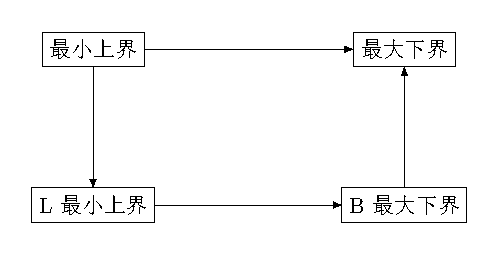
\includegraphics[width=0.7\linewidth]{pic/chap01sec02_proof11.pdf}
        % \caption{function-mapping}
        \label{fig:chap01sec02_proof11}
    \end{figure}

    $L = \{y| y\in S; \forall x\in B, y\leq x\}$
    关于 $L$ 中有没有不在 $S$ 中的元素这一点我还没想明白.
    定理中只是说 $L$ 是 $B$ 的下界组成的. 
    $B$ 是 $S$ 的子集, 但 $B$ 的下界不一定全在 $S$ 中. 

    $L$ 由 $B$ 在 $S$ 中的全部下界组成

    $\forall x\in B$, $x$ 为 $L$ 的上界. $L\subset S$.
    $S$ 有最小上界性质,
    $\therefore \exists \alpha\in S$, $\alpha = \sup L$.

    $\forall \gamma <\alpha$ 由 $\alpha = \sup L$ 的定义 (\ref{mydef:1.8})
    $\gamma$ 不是 $L$ 的上界.

    $\forall x \in B$, $x$ 为 $L$ 的上界, $x \geq \alpha$. $\therefore \alpha \in L$.

    $\alpha < \beta$, $\alpha = \sup L$. $\therefore \beta \not\in L$.
    $L$ 由 $B$ 在 $S$ 中的全部下界组成, $\beta \not\in L$.
    $\beta$ 不是 $B$ 的下界.

    $\therefore \alpha = \inf B$, $\inf B\in S$.
\end{proof}



\section{Fields}
\mybox{
    域, 交换除环 <$\R,+,\times$> 
    <$\R,+$>, <$\R\backslash\{0\},\times$>
    都是交换群, 且满足分配律. 

    则 <$\R,+,\times$> 是域. 
}

\begin{mydef}\label{mydef:1.12}
% Axiom % 公理

(A) Axioms for addition
\begin{enumerate}[(\text{A}1)]
    \item If $x\in F$  and $y \in F$, then their sum \(x + y\) is in F.
    \item Addition is commutative: \(x + y=y+ x\) for all \(x, y \in F\).
    \item Addition is associative: \((x+ y)+z = x + (y+ z)\) for all \(x, y, z \in F\).
    \item $F$ contains an element $0$ such that $0 + x = x$ for every $x \in F$.
    \item To every $x\in F$ corresponds an element $-x\in F$ such that
\end{enumerate}
\begin{equation*}
    x+(-x)=0.
\end{equation*}

(M) Axioms for multiplication
\begin{enumerate}[(\text{M}1)]
    \item If $x\in F$ and $x\in F$, then their product $xy$ is in $F$.
    \item Multiplication is commutative: $xy = yx$ for all $x, y \in  F$.
    \item Multiplication is associative: $(xy)z = x(yz)$ for all $x, y, z \in  F$.
    \item $F$ contains an element $1 \neq 0$ such that $1x = x$ for every $x \in F$.
    \item If $x \in F$ and $x \neq 0$ then there exists an element $1/x \in F$ such that
\end{enumerate}
\begin{equation*}
    x\cdot(1/x)=1.
\end{equation*}


(D) The distributive law
\begin{equation*}
    x(y+z)=xy+ xz
\end{equation*}

holds for all $x, y, z \in F$.
\end{mydef}

\begin{myremark}
    \label{myremark:1.13}
    \begin{enumerate}[(a)]
        \item Our usual writes (in any filed) $x-y = x+(-y)$, $x/y=x\cdot (1/y)$.
        \item The field axioms clearly hold in $\Q $, 
        the set of all rational numbers, 
        if addition and multiplication have their customary meaning. 
        Thus $\Q $ is a field.
        \item Although it is not our purpose to study fields 
        (or any other algebraic structures) in detail, 
        it is worthwhile to prove that some familiar properties of $\Q $ are consequences of the field axioms; 
        once we do this, we will \underline{not need to do it} again for the real numbers and for the complex numbers.
    \end{enumerate}
\end{myremark}
 
\mybox{
    \begin{inparaenum}
        \item 只定义了加法和乘法, 使用逆元分别表示减法和除法.
        \item 全体有理数的集合是一个域.
    \end{inparaenum}
}


\begin{myProposition}
    \label{myProposition:1.14}
    The axioms for addition imply the following statements.
    \begin{enumerate}[(a)]
        \item If $x+y=x+z$ then $y=z$.
        \item If $x+y=x$ then $y=0$.
        \item If $x+y=0$ then $y= -x$.
        \item $-(-x)=x$.
    \end{enumerate}
\end{myProposition}

Statement (a) is a cancellation law. 
Note that (b) asserts the uniqueness of the element 
whose existence is assumed in (A4), 
and that (c) does the same for (A5).

\mybox{
    what is the difference between axiom and proposition?

    An axiom is a proposition regarded as self-evidently true without proof. 
    The word ``axiom'' is a slightly archaic synonym for postulate. 
    Compare conjecture or hypothesis, 
    both of which connote apparently true but not self-evident statements.
    
    A proposition is a mathematical statement such as 
    ``3 is greater than 4,'' 
    ``an infinite set exists,''
    or 
    ``7 is prime.''
    
    An axiom is a proposition that is assumed to be true. 
    With sufficient information, m
    athematical logic can often categorize a proposition as true or false, 
    although there are various exceptions 
    (e.g., 
    ``This statement is false''
    ).
    
    \url{https://www.nutritionmodels.com/terminology.html}
}


\begin{proof}
    Proof(rudin)
    If $x + y =x + z$, the axioms (A) give
    \begin{align*}
        y =0+y&=(-x+x)+y=-x+(x+y)\\
        &=-x+(x+z)=(-x+x)+z=0+z=z
    \end{align*}

    This proves (a). Take $z = 0$ in (a) to obtain (b). 
    Take $z= -x$ in (a) to obtain (c).
    Since $-x + x = 0$, (c) (with $-x$ in place of $x$) gives (d).
\end{proof}

\mybox{
    我自己证明上述四条性质时都是从定义开始的, 
    而 rudin 这里在后一步的证明中都利用了刚推导出的结论, 
    这一点需要借鉴.
    }
% THE REAL AND COMPLEX NUMBER SYSTEMS 7

\begin{myProposition}
    \label{myProposition:1.15}
    The axioms for multiplication imply the following statements.
    \begin{enumerate}[(a)]
        \item If $x\neq0$ and $xy=xz$ then $y=z$.
        \item If $x\neq0$ and $xy=x$ then $y=1$.
        \item If $x\neq0$ and $xy=1$ then $y=1/x$.
        \item If $x\neq0$ then $1/(1/x) = x$.
    \end{enumerate}
\end{myProposition}

The proof is so similar to that of Proposition \ref{myProposition:1.14} that we omit it.


\begin{proof}
    \begin{asparaenum}[(a)]
        \item ,
        \begin{align*}
            y&=1\cdot y=\left(\frac{1}{x}\cdot x\right)y =\frac{1}{x}\left( xy \right)\\
            &=\frac{1}{x}(xz) =\left(\frac{1}{x}x\right)z = z
        \end{align*}
        \item (a)Let $z=1$. $y=z=1$.
        \item (a)Let $z=\frac{1}{x}$. $y=z=\frac{1}{x}$.
        \item (c)Let $x=\frac{1}{x'}$. $y=1/(1/x')$.
    \end{asparaenum}
\end{proof}

\begin{myProposition}
    \label{Proposition:1.16}
    The field axioms imply the following statements, for any $x, y, z \in F$.
    \begin{enumerate}[(a)]
        \item $0x=0$.
        \item If $x\neq 0$ and $y\neq 0$ then $xy\neq 0$.
        \item $(-x)y=-(xy)=x(-y)$.
        \item $(-x)(-y)=xy$.
    \end{enumerate}
\end{myProposition}

\begin{proof}
    $0x+0x=(0+0)x=0x$. Hence \ref{myProposition:1.14}(b) implies that $0x=0$, and (a) holds.

    Next, assume $x \neq 0$, $y \neq 0$, but $xy =0$. Then (a) gives
    \begin{equation*}
        1=
        \left(\frac{1}{y}\right)\left(\frac{1}{x}\right)xy=
        \left(\frac{1}{y}\right)\left(\frac{1}{x}\right)0=0.
    \end{equation*}

    a contradiction. Thus (b) holds.

    The first equality in (c) comes from
    \begin{equation*}
        (-x)y +xy=(-x+x)y=0y=0,
    \end{equation*}

    combined with \ref{myProposition:1.14}(c); 
    the other half of (c) is proved in the same way.\\
    Finally,
    \begin{equation*}
        (-x)(-y)=-[x(-y)]=-[-(xy)]=xy
    \end{equation*}
    by (c) and \ref{myProposition:1.14}(d).
\end{proof}

\begin{mydef}
    \label{mydef:1.17}
    An ordered field is a field $F$ which is also an ordered set, 
    such that
    \begin{enumerate}[(i)]
        \item $x+y<x+z$ if $x,y,z\in F$ and $y<z$,
        \item $xy>0$ if $x\in F$, $y\in F$, $x>0$, and $y>0$.
    \end{enumerate}
\end{mydef}

If $x > 0$, we call $x$ positive; 

if $x < 0$, $x$ is negative.

For example, $\Q $ is an ordered field.

All the familiar rules for working with inequalities apply in every ordered
field: 
Multiplication by positive [negative] quantities preserves [reverses] inequalities, no square is negative, etc. 
The following proposition lists some of these.

\mybox{
    有序域$F$也是有序集, 
    由于有理数域 $\Q $, 实数域 $\R$ 都是有序域, 
    这里使用有理数域 $\Q $ 证明的有序集的性质也可以直接用于实数域 $\R$.}

\begin{myProposition}
    \label{myProposition:1.18}
    The following statements are true in every ordered field.
    \begin{enumerate}[(a)]
        \item If $x>0$ then $-x <0$, and vice versa.
        \item If $x>0$ and $y<z$ then $xy <xz$.
        \item If $x<0$ and $y<z$ then $xy> xz$.
        \item If $x \neq 0$ then $x^2 > 0$. In particular, $1 > 0$.
        \item If $0<x<y$ then $0<l/y<l/x$.
    \end{enumerate}
\end{myProposition}

\begin{proof}
    \begin{asparaenum}[(a)]
    \item $x>0$, $-x<0$. 
    \begin{align*}
        x   &> 0=(x+-x)\\
        x+0 &> x+(-x)\\
        (-x)&<0
    \end{align*}

    \item $x>0$, $y<z$, $xy<xz$.
    \begin{align*}
        y<z, z-y&>y-y=0\\
        x(z-y)&>0\\
        x(z-y)+xy&>0+xy\\
        xz&>xy
    \end{align*}

    \item
    \begin{align*}
        (z-y) &>y-y=0\\
        x<0,(-x)>0.\quad (-x)(z-y)&>0 \\
        x(z-y) &<0\\
        xz<xy    
    \end{align*}

    \item
    \begin{align*}
        x>0  && x^2    >0  \\
        x<0  &&(-x)^2 >0, (-x)^2 = -[x(-x)] = -(-(x\cdot x)) =x^2, x^2>0
    \end{align*}
    $\because 1^2=1$, $1>0$.

    \item
    If $y>0$ and $v \leq 0$, then $yv \leq 0$. 
    But $y \cdot (1/y)=1>0$. Hence $1/y > 0$.
    Likewise, $1/x > 0$. 
    If we multiply both sides of the inequality $x <y$ by
    the positive quantity $(1/x)(1/y)$, we obtain $1/y <1/x$.
    \end{asparaenum}
\end{proof}



\section{The real field}

We now state the \myKeywordblue{existence theorem} which is the core of this chapter.

\begin{thm}
    \label{thm:1.19}
    There exists an \myKeywordblue{ordered field} $\R$
    which has the least-upper-bound property.

    Moreover, $\R$ contains $\Q $ as a \myKeywordblue{subfield}.
\end{thm}

The second statement means that $\Q \subset \R$
and that the operations of addition and multiplication in $\R$,
when applied to members of $\Q $,
coincide with the usual operations on rational numbers;
also, the positive rational numbers are positive elements of $\R$.

The members of $\R$ are called \myKeywordblue{real numbers}.

The proof of Theorem \ref{thm:1.19} is rather long and a bit tedious
and is therefore presented in an Appendix to Chap.
1 .
% Appendix\ref{chap01_app}.
The proof actually constructs $\R$ from $\Q$.

The next theorem could be extracted from this construction with very little extra effort.
However, we prefer to derive it from Theorem \ref{thm:1.19} since this
provides a good illustration of what one can do with the least-upper-bound property.

\mybox{$\R$ 具有最小上界性质的有序域
    least-upper-bound $\rightarrow$ upper bound in the sets.
    ordered field (ordered set, field).

    $\Q \in \R$ subfield

    $x\in \R$, $x$ is a real number
}
\mybox{
    proof of theorem \ref{thm:1.19} is tedious.
    construct $\R$ from $\Q $

    tedious 乏味的, 冗长的\\
    derive 取得, 得到
}

\begin{thm}
    \label{thm:1.20}
    \myKeywordred{(archimedean property of $\R$)}
    (a) If $x \in \R$, $y \in \R$, and $x > 0$, then there is a positive integer $n$ such that
    \begin{equation*}
        nx > y
    \end{equation*}

    (b) If $x \in \R$, $y \in \R$, and $x < y$, then there exists a $p \in Q$ such that $x < p < y$.
\end{thm}
\mybox{阿基米德公理

    \url{https://mathworld.wolfram.com/ArchimedesAxiom.html}

    Archimedes' axiom, also known as the continuity axiom or Archimedes' lemma, survives in the writings of Eudoxus (Boyer and Merzbach 1991), but the term was first coined by the Austrian mathematician Otto Stolz (1883). It states that, given two magnitudes having a ratio, one can find a multiple of either which will exceed the other. This principle was the basis for the method of exhaustion, which Archimedes invented to solve problems of area and volume.

    Symbolically, the axiom states that
    $a/b=c/d$

    iff the appropriate one of following conditions is satisfied for integers $m$ and $n$:
    \begin{enumerate}[1. ]
        \item If $ma < nb$, then $mc < nd$.
        \item If $ma = nb$, then $mc = nd$.
        \item If $ma > nb$, then $mc > nd$.
    \end{enumerate}

    Formally, Archimedes' axiom states that if $AB$ and $CD$ are two line segments, then there exist a finite number of points $A_1, A_2, ..., A_n$ on $A$ union $B$ such that
    \[CD \equiv AA_1 \equiv A_1A_2 \equiv ... \equiv A_{(n-1)}A_n,\]

    and $B$ is between $A$ and $A_n$ (Itô 1986, p.611).
    A geometry in which Archimedes' lemma does not hold is called a non-Archimedean Geometry.
}

\begin{proof}
    \begin{asparaenum}[(a)]
        \item Let $A$ be the set of all $nx$,
        where $n$ runs through the positive integers.
        If (a) were false, then $y$ would be an upper bound of $A$.
        But then $A$ has a \emph{least} upper bound in $\R$.
        Put $\alpha = \sup A$.
        Since $x > 0$, $\alpha - x < \alpha$,
        and $\alpha - x$ is not an upper bound of $A$.
        Hence $\alpha - x < mx$ for some positive integer $m$.
        But then $\alpha < (m + l)x \in A$,
        which is impossible,
        since $\alpha$ is an upper bound of $A$.
        \item Since $x < y$, we have $y - x > $0,
        and (a) furnishes a positive integer $n$
        such that
        \begin{equation*}
            n(y - x) > 1.
        \end{equation*}
        Apply (a) again, to obtain positive integers $m_1$ and $m_2$
        such that $m_1 > nx$, $m_2 > -nx$.

        Then
        \begin{equation*}
            -m_2 < nx < m_1
        \end{equation*}
        Hence there is an integer $m$ (with $-m_2 \leq m \leq m_1$)
        such that
        \begin{equation*}
            m - 1\leq n x < m.
        \end{equation*}
        If we combine these inequalities, we obtain
        \begin{equation*}
            nx < m \leq 1 + nx < ny.
        \end{equation*}
        Since $n > 0$, it follows that
        \begin{equation*}
            x < \frac{m}{n} < y.
        \end{equation*}
        This proves (b), with $p = m/n$.
    \end{asparaenum}
\end{proof}

We shall now prove the existence of nth roots of positive reals.
This proof will show how the difficulty pointed out in the Introduction
(irrationality of $\sqrt{2}$) can be handled in $\R$.

\begin{thm}
    \label{thm:1.21}
    For every real $x > 0$ and every integer $n> 0$
    there is one and only one positive real $y$
    such that $y^n = x$.
\end{thm}

This number $y$ is written $\sqrt[n]{x}$ or $x^{1/n}$.
\mybox{
    这里定义了$n$次根式, 最开始根式由二次方程的解引出, 将根式作为次方项处理.
    有理数根式可以视为两个整数之比, 次方与开根号的顺序可以交换.
    实数根式则视为有理数根式构成的序列的极限值.
    复数根式需要通过欧拉公式 $e^{ix} = \cos x + i \sin x$ 理解.
}
\begin{proof}
    That there is at most one such $y$ is clear,
    since $0 < y_1 < y_2$ implies $y_1^n < y_2^n$.

    Let $E$ be the set consisting of all positive real numbers $t$
    such that $t^n < x$.

    If $t = x/(1 + x)$ then $0 \leq t < 1$.
    Hence $t^{n} \leq t < x$.
    Thus $t \in E$, and $E$ is not empty.

    If $t > 1 + x$ then $t^{n} \geq t > x$,
    so that $t \not\in E$.
    Thus $1 + x$ is an upper bound of $E$.

    Hence Theorem \ref{thm:1.19} implies the existence of
    \begin{equation*}
        y = \sup E.
    \end{equation*}
    To prove that $y^{n} = x$ we will show that
    each of the inequalities $y^{n} < x$ and $y^{n} > x$ leads to a contradiction.

    The identity $b^{n} - a^{n}= (b - a)(b^{n-1} + b^{n}- 2a + \cdots + a^{n-1})$ yields the inequality
    \begin{equation*}
        b^{n} - a^{n} < (b - a)nb^{n-1}
    \end{equation*}
    when $0 < a < b$.

    Assume $y^{n} < x$. Choose $h$ so that $0 < h < 1$ and
    \begin{equation*}
        h < \frac{x - y^n}{n(y + 1)^{n-1}}.
    \end{equation*}
    Put $a = y$, $b = y + h$. Then
    \begin{equation*}
        (y + h)^{n} - y^{n}
        < hn(y + h)^{n-l}
        < hn(y + l)^{n-1}
        < x - y^{n}.
    \end{equation*}
    Thus $(y + h)^{n} < x$, and $y +h \in E$.
    Since $y + h > y$,
    this contradicts the fact that $y$ is an upper bound of $E$.

    Assume $y^{n} > x$. Put
    \begin{equation*}
        k = \frac{y^n - x}{n y^{n-1}}
    \end{equation*}
    Then $0 < k < y$.
    If $t \leq y - k$, we conclude that
    \begin{equation*}
        y^{n} - t^{n}
        \leq y^{n} - (y - k)^{n}
        < kny^{n-1}
        = y^{n} - x.
    \end{equation*}
    Thus $t^{n} > x$, and $t \not\in E$.
    It follows that $y - k$ is an upper bound of $E$.
    But $y - k < y$,
    which contradicts the fact that $y$ is the least upper bound of $E$.
    Hence $y^{n} = x$, and the proof is complete.
\end{proof}
\mybox{
    很经典的等式证明,
    从两边的不等式不成立出发证明有且仅有等式成立.
}

\begin{myCorollary*}
    If $a$ and $b$ are positive real numbers
    and $n$ is a positive integer,
    then
    \begin{equation*}
        (ab)^{1/n}= a^{1/n}b^{1/n}.
    \end{equation*}
\end{myCorollary*}

\begin{mydef}
    \label{mydef:1.22}
    \myKeywordblue{(Decimals)}
    We conclude this section by pointing out the relation between real numbers and decimals.
\end{mydef}



\section{The extended real number system}
\mybox{使用正负无穷大扩充实数系}
\begin{mydef}
    \label{thm:1.23}
    The extended real number system consists of the real field $\R$
    and two symbols, $+\infty$ and $-\infty$. 
    We preserve the original order in $\R$, 
    and define
    \begin{equation*}
        -\infty <x<+\infty
    \end{equation*}
    for every $x\in \R$
\end{mydef}

\begin{asparaenum}[(a)]
\item If $x$ is real then
\begin{equation*}
    x+\infty = +\infty,\quad
    x-\infty = -\infty,\quad
    \frac{x}{+\infty}=\frac{x}{-\infty}=0.
\end{equation*}

\item If $x>0$ 
then $x\cdot (+\infty) = +\infty$, 
$x\cdot(-\infty)=-\infty$.

\item If $x<\infty$ 
then $x\cdot(+\infty)=-\infty$, 
$x\cdot(-\infty)= +\infty$.
\end{asparaenum}



\section{The complex field}

\mybox{
    rudin 引入复数定义的方法很奇怪, 
    使用复数的代数定义直接引入(天上掉下来的定义).
    理解起来比较困难.

    我觉得使用几何方法引入复数更为合理且直观, 
    rudin 这里对初学者不太友好.
}

\begin{mydef}
    \label{mydef:1.24}
    A complex number is an ordered pair $(a, b)$ of real numbers.
    ``Ordered'' means that $(a, b)$ and $(b, a)$ are regarded as distinct if $a \neq b$.

    Let$x = (a, b)$, $y = (c,d)$ be two complex numbers. 
    We write $x =y$ if and only if $a =c$ and $b=d$. 
    (Note that this definition is not entirely superfluous;
    think of equality of rational numbers, 
    represented as quotients of integers.) 
    We define
    \begin{align*}
        x+y &= (a + c, b + d),\\
        xy  &= (ac - bd, ad + bc).
    \end{align*}
\end{mydef}

\begin{thm}
    \label{thm:1.25}
    These definitions of addition and multiplication 
    turn the \emph{set} of all complex numbers into a field, 
    with $(0, 0)$ and $(1, 0)$ in the role $0$ and $1$.
\end{thm}

\mybox{
    proof (A1) $\sim$ (A5), (M1) $\sim$ (M5) and (D), 

    then we can prove that $\mathbb{C}$ is a field.
}

\begin{thm}
    \label{thm:1.26}
    For any real numbers $a$ and $b$ we have
    \begin{equation*}
        (a,0)+ (b,0) = (a+ b,0),\quad
        (a,0)(b,0) = (ab,0).
    \end{equation*}
\end{thm}
The proof is trivial.

show that the notation $(a, b)$ is equivalent to the more customary $a + bi$.

\begin{mydef}
    \label{mydef:1.27}
    $i=(0,1)$    
\end{mydef}

\begin{thm}
    \label{thm:1.28}
    $i^2=-1$
\end{thm}

\begin{proof}
    \begin{equation*}
        i^2=(0,1)(0,1)=(-1,0)=-1.
    \end{equation*}
\end{proof}

\begin{thm}
    \label{thm:1.29}
    If $a$ and $b$ are real, then $(a,b) =a + bi$.
\end{thm}

\begin{proof}
    \begin{align*}
        a+bi
        &=(a,0)+(b,0)(0,1)\\
        &=(a,0)+(0,b)=(a,b)\\
    \end{align*}
\end{proof}

\begin{mydef}
    \label{mydef:1.30}
    $a,b\in \R$, $z = a + bi$,
    the complex number $\bar{z} = a  -bi$ is called the conjugate of $z$.
    the numbers $a$ and $b$ are the real part and imaginary part of $z$.
    respectively.
    \begin{equation*}
        a=\Re(z), \quad
        b=\Im(z)
    \end{equation*}
\end{mydef}

\begin{thm}
    \label{thm:1.31}
    If $z$ and $w$ are complex, then
    \begin{enumerate}[(a)]
        \item $\bar{z+w}=\bar{z}+\bar{w}$,
        \item $\bar{zw}=\bar{z}\cdot\bar{w}$,
        \item $z+\bar{z}=2\Re(z)$, $z-\bar{z}=2\Im(z)$,
        \item $z\bar{z}$ is real and positive (except when $z=0$).
    \end{enumerate}
\end{thm}

\begin{proof}
    (a), (b),and (c)are quite trivial.
    To prove (d), write $z = a + bi$,
    and note that $z\bar{z} = a^2 + b^2$.
\end{proof}


\begin{mydef}
    \label{mydef:1.32}
    If $z$ is a complex number, 
    its absolute value $|z|$ is the nonnegative square root of $z\bar{z}$; 
    that is, $|z| = (z\bar{z})^{1/2}$.
\end{mydef}
The existence (and uniqueness) of $|z|$ follows from Theorem \ref{thm:1.21} and part (d) of Theorem \ref{thm:1.31}.

Note that when $x$ is real, then $\bar{x} = x$, 
hence $|x| = \sqrt{x^2}$. Thus $|x| = x$
if $x>0$, $|x| = -x$ if $x <0$.


Properties of complex number.

\begin{thm}
    \label{thm:1.33}
    Let $z$ and $w$ be complex numbers. Then
    \begin{enumerate}[(a)]
        \item $|z|>0$ unless $z=0$, $|0|=0$,
        \item $\bar{z}=z$,
        \item $|zw| = |z||w|$,
        \item $| \Re(z)| \leq |z|$,
        \item $|z+w| \leq|z|+|w|$.
    \end{enumerate}
\end{thm}


\begin{myNotation}\myKeywordred{(Big sum)}
    \label{myNotation:1.34}
    $x_1,x_2,\dots,x_n \in \mathbb{C}$,
    \begin{equation*}
        x_1+x_2+\dots+x_n = \sum_{j=1}^{n} x_j.
    \end{equation*}
\end{myNotation}

\begin{thm}\myKeywordred{(Schwarz Inequality)}
    \label{thm:1.35}
    If 
    $a_1,\dots,a_n$, 
    $b_1,\dots,b_n$, are complex numbers, then
    \begin{equation*}
        \left| \sum_{j=1}^{n}a_j \bar{b_j}\right|^2 \leq 
        \sum_{j=1}^{n}\left|a_j\right|^2
        \sum_{j=1}^{n}\left|b_j\right|^2.
    \end{equation*}    
\end{thm}

\mybox{在正式证明之前, 先回忆 $\R$ 中的施瓦茨不等式是怎么证明的.}
\begin{proof}
    let $A = \sum a_j^2$, $B = \sum b_j^2$, $C = \sum a_j b_j$.
    \begin{equation*}
        \sum (a_j+\lambda b_j)^2 = 
        \sum a_j^2 
        + 2\sum a_j b_j \lambda
        + \sum b_j^2 \lambda^2
    \end{equation*}
    由韦达定理, $\Delta \leq 0$, 
    $\Delta= (2\sum a_j b_j )^2 - 4 \sum a_j^2\sum b_j^2$. 
    因此 $(\sum a_j b_j )^2 \leq \sum a_j^2\sum b_j^2$.
\end{proof}


\begin{proof}
    Put $A = \sum |a_j|^2$, $B = \sum |b_j|^2$, $C = \sum a_j \bar{b_j}$, $j = 1,2,\dots,n$. \\    
    If $B = 0$, $b_1 = \dots = b_n = 0$, this conclusion is trivial.\\
    If $B > 0$, 
    \begin{align*}
        \sum \left|B a_j - C b_j\right|^2
        &= \sum (B a_j-C b_j)(B \bar{a_j} - \bar{C b_j})\\
        &= B^2\sum \left|a_j\right|^2 - B\bar{C}\sum a_j \bar{b_j} - BC \sum \bar{a_j} b_j + \left|C\right|^2\sum |b_j|^2\\
        &= B^2A-B|C|^2\\
        &= B(AB-|C|^2).
    \end{align*}
    Since each term in the first sum is nonnegative, we see that
    \begin{equation*}
        B(AB-|C|^2) \geq 0.
    \end{equation*}
    Since $B>0$, it follows that $AB-|C|^2 \geq 0$. This is the desired inequality.
\end{proof}

\mybox{
    \begin{proof}
        我的想法
        \begin{align*}
            \sum (a_j + \lambda \bar{b_j})(\bar{a_j} + \lambda b_j)
            &=\sum(
                a_j\bar{a_j}
                + \lambda(\bar{a_j}b_j+a_j\bar{b_j})
                + \lambda^2 b_j\bar{b_j}
                )\\
            &= A + \lambda (C + \overline{C}) + \lambda^{2} B
        \end{align*}
        由韦达定理, $\Delta \leq 0$, 
        % $\Delta = (\sum\Re(a_j\bar{b_j}))^2-4\sum a_j\bar{a_j}\sum b_j\bar{b_j}$, 
        $\Delta = (C + \overline{C})^2-4AB \leq 0$, 
        (这里推出的结论比原始结论弱?为什么?)
    
        $A = \sum \left| a_j \right|^2 $,
        $B = \sum \left| b_j \right|^2 $,
        $C = \sum a_j \bar{b}_j$.
        \begin{align*}
            \left| C \right|^2 
            &= C \cdot \overline{C}\\
            &= \left( \sum a_j \bar{b}_j \right) 
            \overline{\left( \sum a_j \bar{b}_j \right)}.\\
            &= \left( \sum a_j \bar{b}_j \right) 
            \left( \sum \overline{a_j \bar{b}_j} \right).\\
            &= \left( \sum a_j \bar{b}_j \right) 
            \left( \sum \bar{a}_j {b}_j \right).
        \end{align*}
    
        可不可以用 $C^2 + \overline{C}^2 \geq 2 C \overline{C}$?
    \end{proof}
}
\section{Euclidean space}
\mybox{欧式空间}

\begin{mydef}
    \label{mydef:1.36}
    For each positive integer $k$,
    let $\R^k$ be the set of all ordered $k$-tuples
    \begin{equation*}
        \mathbf{x} = \left(x_1,x_2,\dots,x_k\right),
    \end{equation*}
    where $x_1,x_2,\dots,x_k$ are real numbers, called the \emph{coordinates} of $\mathbf{x}$.
    The elements of $\R^k$ are called points, or vectors,
    especially when $k > 1$. We shall denote vectors
    by boldfaced letters.
    If $\mathbf{y} = \left(y_1,y_2,\dots,y_k\right)$
    and if $\alpha$ is a real number, put
    \begin{align*}
        \mathbf{x} + \mathbf{y} & = \left(x_1+y_1,x_2+y_2,\dots,x_k+y_k\right),         \\
        \alpha\mathbf{x}        & = \left(\alpha x_1,\alpha x_2,\dots,\alpha x_k\right)
    \end{align*}
    so that $\mathbf{x} +\mathbf{y} \in \R^k$ and $\alpha\mathbf{x} \in \R^k$.
    This defines addition of vectors,
    as well as multiplication of a vector by a real number (a scalar).
    These two operations satisfy the commutative, associative,
    and distributive laws
    (the proof is trivial, in view of the analogous laws for the real numbers)
    and make $\R^k$ into a vector space over the \emph{real field}.
    The zero element of $\R^k$ (sometimes called the origin or the null vector) is the point $\mathbf{0}$,
    all of whose coordinates are $0$.

    We also define the so-called ``inner product'' (or scalar product) of $\mathbf{x}$ and $\mathbf{y}$ by
    \begin{equation*}
        \mathbf{x}\cdot\mathbf{y} = \sum_{j=1}^{k}x_j y_j
    \end{equation*}
    and the norm of $\mathbf{x}$ by
    \begin{equation*}
        |x| = (x\cdot x)^{1/2} = \left( \sum_{1}^{k} x_j^2 \right)^{1/2}.
    \end{equation*}

    The structure now defined (the vector space $\R^k$ with the above inner product and norm) is called euclidean $k$-space.
\end{mydef}

\begin{thm}\label{thm:1.37}
    Suppose $\mathbf{x}, \mathbf{y}, \mathbf{z}\in\R^k$, and $\alpha$ is real. Then
    \begin{enumerate}[(a)]
        \item $| \mathbf{x}| \geq 0$;
        \item $| \mathbf{x}| = 0$ if and only if $\mathbf{x} =0$;
        \item $| \alpha \mathbf{x}| = | \alpha||x|$
        \item $|\mathbf{x}\cdot\mathbf{y}| \leq  |\mathbf{x}| | \mathbf{y}|$;
        \item $|\mathbf{x}+\mathbf{y}| \leq | \mathbf{x} | + | \mathbf{y}|$;
        \item $|\mathbf{x}-\mathbf{z}| \leq |\mathbf{x}-\mathbf{y}| + |\mathbf{y}-\mathbf{z}|$.
    \end{enumerate}
\end{thm}

\mybox{(e) 为欧式空间中的三角不等式. }

\begin{proof}
    Proof (a), (b), and (c) are obvious, and (d) is an immediate consequence of the Schwarz inequality\ref{thm:1.35}.
    By (d) we have
    \begin{align*}
        |\mathbf{x} + \mathbf{y}|^2
         & = (\mathbf{x} + \mathbf{y}) \cdot (\mathbf{x} + \mathbf{y})                                \\
         & = \mathbf{x} \cdot \mathbf{x} + 2\mathbf{x} \cdot \mathbf{y} + \mathbf{y} \cdot \mathbf{y} \\
         & \leq |\mathbf{x}|^2 + 2|\mathbf{x}||\mathbf{y}| + |\mathbf{y}|^2                           \\
         & = \left(|\mathbf{x}| + |\mathbf{y}|\right)^2.
    \end{align*}
    so that (e) is proved. Finally,
    (f) follows from (e) if we
    replace $\mathbf{x}$ by $\mathbf{x}-\mathbf{y}$
    and $\mathbf{y}$ by $\mathbf{y}-\mathbf{z}$.
\end{proof}

\begin{myremark}
    \label{myremark:1.38}
    Theorem \ref{thm:1.37} (a), (b), and (f) will allow us (see Chap. 2
    % \ref{chap:02}
    ) to
    regard $\R^k$ as a metric space.

    $\R^1$ (the set of all real numbers) is usually called the line,
    or the real line.
    Likewise, $\R^2$ is called the plane, or the complex plane (compare Definitions \ref{mydef:1.24} and \ref{mydef:1.36}).
    In these two cases the norm is just the absolute value of the corresponding real or complex number.
\end{myremark}

% chap01appendix.tex
\section*{appendix}
\label{chap01_app}
Theorem \ref{thm:1.19} will be proved in this appendix
by constructing $\R$ from $\Q$.
We shall divide the construction into several steps.

\myKeyword{Step 1}
\label{chap01_app_Step:1}
The members of $\R$ will be certain subsets of $\Q$, called \myKeywordblue{cuts}.
A cut is, by definition,
any set $\alpha \subset \Q$ with the following three properties.
\begin{enumerate}[(I)]
    \item $\alpha$ is not empty, and $\alpha \neq \Q$.
    \item If $p\in \alpha$,$q \in \Q$, and $q <p$, then $q \in \alpha$.
    \item If $p \in \alpha$, then $p <r$ for some $r\in \alpha$.
\end{enumerate}
\mybox{分划 $\alpha$ 是一个集合}

The letters $p, q, r, ...$ will always denote rational numbers,
and $\alpha, \beta, \gamma, ...$ will denote cuts.
\mybox{建立分划定义的这三条性质说明了有理数集是稠密而不是连续的}

Note that (III) simply says that a has no largest member:
(II) implies two facts which will be used freely:

If $p\in\alpha$ and $q\not\in\alpha$ then $p<q$.

If $r\not\in \alpha$ and $r<s$ then $s\not\in \alpha$.

\myKeyword{Step 2}
\label{chap01_app_Step:2}
Define ``$\alpha < \beta$'' to mean:
$\alpha$ is a proper subset of $\beta$.
\mybox{这里使用真子集关系定义了分划(集合)间的序}

Let us check that this meets the requirements of Definition \ref{mydef:1.5}.

If $\alpha < \beta$ and $\beta < \gamma$ it is clear that $\alpha < \gamma$.
(A proper subset of a proper subset is a proper subset.)
It is also clear that at most one of the three relations
\begin{equation*}
    \alpha < \beta, \qquad
    \alpha = \beta, \qquad
    \beta < \alpha.
\end{equation*}
can hold for any pair $\alpha, \beta$.
To show that at least one holds, assume that the first two fail.
Then $\alpha$ is not a subset of $\beta$.
Hence there is a $p \in \alpha$ with $p \not\in \beta$.
If $q \in \beta$, it follows that $q <p$ (since $p \not\in \beta$),
hence $q \in \alpha$, by (II).
Thus $\beta \subset \alpha$.
Since $\beta \neq \alpha$, we conclude: $\beta < \alpha$.

Thus $\R$ is now an ordered set.

\mybox{利用集合关系定义的偏序关系具有传递性和三歧性}

\myKeyword{Step 3}
\label{chap01_app_Step:3}
The ordered set $\R$ has the least-upper-bound property.

To prove this, let $A$ be a nonempty subset of $\R$,
and assume that $\beta \in \R$ is an upper bound of $A$.
Define $\gamma$ to be the union of all $\alpha \in A$.
In other words, $p \in \gamma$ if and only if $p \in \alpha$ for some $\alpha \in A$.
We shall prove that $\gamma \in \R$ and that $\gamma = \sup A$.

Since $A$ is not empty, there exists an $a_0 \in A$.
This $\alpha_0$ is not empty.
Since $\alpha_0 \in \gamma$, $\gamma$ is not empty.
Next, $\gamma \subset \beta$
(since $\alpha \subset \beta$ for every $\alpha \in A$),
and therefore $\gamma \neq \Q$.
Thus $\gamma$ satisfies property (I).
To prove (II) and (III), pick $p \in \gamma$.
Then $p \in \alpha_1$ for some $\alpha_1 \in A$.
If $q <p$, then $q \in \alpha_1$, hence $q \in \gamma$; this proves (II).
If $r \in \alpha_1$ is so chosen that $r > p$,
we see that $r\in \gamma$ (since $\alpha_1 \subset \gamma$),
and therefore $\gamma$ satisfies (III).

Thus $\gamma \in \R$.

It is clear that $\alpha \leq \gamma$ for every $\alpha \in A$.

Suppose $\delta < \gamma$.
Then there is an $s \in \gamma$ and that $s \not\in \delta$.
Since $s \in \gamma, s \in \alpha$ for some $\alpha \in A$.
Hence $\delta <a$, and $\delta$ is not an upper bound of $A$.

This gives the desired result: $\gamma = \sup A$.

\mybox{
    这里分划之间所用的 $\in$ 让我很费解,
    上文对分划的定义是集合, 那么应该用子集形式而不是元素形式来描述偏序关系.
    分划是不是集合的一个元素?

    查询原始pdf文件发现确实是子集形式描述的!
}

\myKeyword{Step 4}
\label{chap01_app_Step:4}
If $\alpha \in \R$ and $\beta \in \R$
we define $\alpha + \beta$ to be the set of all sums $r + s$,
where $r \in \alpha$ and $s \in \beta$.

We define $0^*$ to be the set of all negative rational numbers.
It is clear that $0^*$ is a cut.
We verify that the axioms for addition
(see Definition \ref{mydef:1.12})
hold in $\R$, with $0^*$ playing the role of $0$.

\myKeyword{Step 5}
\label{chap01_app_Step:5}
Having proved that the addition defined in Step 4 satisfies Axioms (A) of Definition \ref{mydef:1.12},
it follows that Proposition \ref{myProposition:1.14} is valid in $\R$, and we can
prove one of the requirements of Definition \ref{mydef:1.17}:

If $\alpha, \beta, \gamma \in \R$ and $\beta < \gamma$, then $\alpha + \beta < \alpha + \gamma$.

Indeed, it is obvious from the definition of $+$ in $\R$ that $\alpha + \beta \subset \alpha + \gamma$;
if we had $\alpha + \beta = \alpha + \gamma$,
the cancellation law (Proposition \ref{myProposition:1.14}) would imply $\beta = \gamma$.

It also follows that $\alpha > 0^*$ if and only if $-\alpha < 0^*$.

\myKeyword{Step 6}
\label{chap01_app_Step:6}
Multiplication is a little more bothersome than addition in the present context,
since products of negative rationals are positive.
For this reason we confine ourselves first to $\R^+$,
the set of all $\alpha \in \R$ with $\alpha > 0^*$.

If $\alpha \in \R^+$ and $\beta \in \R^+$,
we define $\alpha\beta$ to be the set of all $p$ such that $p \leq rs$
for some choice of $r \in \alpha$, $s \in \beta$, $r>0$, $s>0$.

We define $1^*$ to be the set of all $q < 1$.

Then the axioms (M) and (D) of Definition \ref{mydef:1.12} hold,
with $\R^+$ in place of $F$, and with $1^*$ in the role of $1$.

The proofs are so similar to the ones given in detail in Step 4 that we omit them.

Note, in particular, that the second requirement of Definition \ref{mydef:1.17} holds:
If $\alpha > 0^*$ and $\beta > 0^*$ then $\alpha\beta > 0^*$.

\myKeyword{Step 7}
\label{chap01_app_Step:7}
We complete the definition of multiplication
by setting $\alpha 0^* = 0^* \alpha = 0^*$,
and by setting
\begin{equation*}
    \alpha\beta = \left\{
    \begin{array}{ll}
        (-\alpha)(-\beta)      & \text{if } \alpha < 0^*, \beta < 0^*, \\
        -[(-\alpha)\beta]      & \text{if } \alpha < 0^*, \beta > 0^*, \\
        -[\alpha\cdot(-\beta)] & \text{if } \alpha > 0^*, \beta < 0^*, \\
    \end{array}
    \right.
\end{equation*}
The products on the right were defined in Step 6.

Having proved (in Step 6) that the axioms (M) hold in $\R^+$,
it is now perfectly simple to prove them in$\R^+$,
by repeated application of the identity $\gamma = -(-\gamma)$
which is part of Proposition \ref{myProposition:1.14}. (See Step 5.)

The proof of the distributive law
\begin{equation*}
    \alpha(\beta + \gamma) = \alpha\beta + \alpha\gamma
\end{equation*}
breaks into cases.
For instance, suppose $\alpha> 0^*$, $\beta <0^*$, $\beta + \gamma > 0^*$
Then $\gamma = (\beta + \gamma) + (- \beta)$,
and (since we already know that the distributive law holds in $\R^+$)
\begin{equation*}
    \alpha\gamma = \alpha(\beta+\gamma) + \alpha \cdot (-\beta).
\end{equation*}
But $\alpha \cdot (-\beta) = -(\alpha\beta)$. Thus
\begin{equation*}
    \alpha\beta + \alpha\gamma = \alpha(\beta + \gamma).
\end{equation*}
The other cases are handled in the same way.

We have now completed the proof that
$\R$ is an ordered-field with the least-upper-bound property.

\myKeyword{Step 8}
\label{chap01_app_Step:8}
We associate with each $r\in \Q$ the set $r^*$
which consists of all $p \in \Q$ such that $p < r$.
It is clear that each $r^*$ is a cut;
that is, $r^* \in \R$.
These cuts satisfy the following relations:
\begin{enumerate}[(a)]
    \item $r^* + s^* = (r+s)^*$,
    \item $r^* s^* = (rs)^*$,
    \item $r^* < s^*$ if and only if $r < s$.
\end{enumerate}

To prove (a), choose $p \in r^* + s^*$. Then $p=u+v$, where $u<r$, $v<s$.
Hence $p < r +s$, which says that $p \in (r + s)^*$.

Conversely, suppose $p \in (r+s)^*$. Then $p < r + s$. Choose $t$ so that
$2t = r + s - p$, put
\begin{equation*}
    r' = r - t,
    s' = s - t.
\end{equation*}
Then $r' \in r^*$, $s' \in s^*$, and $p = r' + s'$, so that $p \in r^* + s^*$

This proves (a). The proof of (b) is similar.

If $r < s$ then $r \in s*$, but $r \not\in r^*$;
hence $r^* < s^*$.

If $r^* <s^*$ then there is a $p \in s^*$
such that $p \not\in r^*$
Hence $r < p < s$, so that $r < s$.

This proves (c).

\myKeyword{Step 9}
\label{chap01_app_Step:9}
We saw in Step \ref{chap01_app_Step:8} that the replacement of the rational numbers $r$
by the corresponding ``rational cuts'' $r^* \in \R$ preserves sums, products, and order.
This fact may be expressed by saying that
the ordered field $\Q$ is isomorphic to the ordered field $\Q^*$
whose elements are the rational cuts.
Of course, $r^*$ is by no means the same as $r$,
but the properties we are concerned with (arithmetic and order) are the same in the two fields.

It is this identification of $\Q$ with $\Q^*$ which allows us to regard $\Q$ as a subfield of $\R$.

The second part of Theorem \ref{thm:1.19} is to be understood in terms of this identification.
Note that the same phenomenon occurs when the real numbers are regarded as a subfield of the complex field,
and it also occurs at a much more elementary level, when the integers are identified with a certain subset of $\Q$.

It is a fact, which we will not prove here, that any two ordered-fields with the least-upper-bound property are isomorphic.
The first part of Theorem \ref{thm:1.19} therefore characterizes the real field $\R$ completely.

The books by Landau and Thurston\cite{LANDAU1951} cited in the Bibliography are entirely devoted to number systems.
Chapter \ref{chap:01} of Knopp's\cite{KNOPP1928} book contains a more leisurely description of how $\R$ can be obtained from $\Q$.
Another construction,
in which each real number is defined to be an equivalence class of Cauchy sequences of rational numbers (see Chap. \ref{chap:03}),
is carried out in Sec. 5 of the book by Hewitt and Stromberg\cite{HEWITT1965}.

The cuts in $\Q$ which we used here were invented by Dedekind.
The construction of $\R$ from $\Q$ by means of Cauchy sequences is due to Cantor.
Both Cantor and Dedekind published their constructions in 1872.

% chap01 exercise
\section{Exercises}

Unless the contrary is explicitly stated, all numbers that are mentioned in these exercises are understood to be real.

\begin{myexercise}
    \label{ex:1.1}
    $r \in \Q $, $r \neq 0$, $x \not\in \Q $, $x \in \R$
    $r+x, rx$ $\not\in \Q , \in \R$
\end{myexercise}


\mySolve

if $r+x \in \Q $, there exists $m, n \in \mathbb{N}, n \neq 0$, s.t. $r+x = \frac{m}{n}$.
    $\because r\in \Q $, $r = \frac{p}{q}, p,q \in \mathbb{N}, q \neq 0$.
    \begin{align*}
        r + x &= \frac{m}{n}\\
        \frac{p}{q} + x &= \frac{m}{n}
    \end{align*}
    \begin{equation*}
        x = \frac{m}{n} - \frac{p}{q} = \frac{mq-np}{nq}
    \end{equation*}
    then $x \in \Q $ contradict to the supposition that $x \not\in \Q $

    If $rx \in \Q $, then $rx = \frac{m}{n}, m,n\in \mathbb{N}$, $x = \frac{qm}{pn} \in \Q $, contradictory!

\mybox{supposition 假设}


\begin{myexercise}
    \label{ex:1.2}
    prove that there is no rational number whose square is $12$. 
\end{myexercise}


\mySolve

If $\left(p/q\right)^2 = 12$, $p^2/q^2 = 12$. $p$ must be even, $p = 2m$.
    $(2m)^2/q^2 = 12$, $m^2/q^2=3$. 
    $3$ is a prime number, $m = 3n$, $(3n)^2/q^2 = 3$, $3n^2 = q^2$, $q$ have a factor $3$,
    $\gcd(p,q) = \gcd(m,q) = \gcd(n,q) = 3 \neq 1$, contradict to the fact that $p,q$ are coprime.


\begin{myexercise}
    \label{ex:1.3}
    Prove Proposition \ref{myProposition:1.15}.
\end{myexercise}


\mySolve

\begin{asparaenum}[(a)]
        \item $x \neq 0$, $xy \neq xz$. $x \neq 0$, $\exists 1/x$, $1/x\cdot x = 1$.
        \begin{align*}
            y & = \left(\frac{1}{}x \cdot x\right) y = \frac{1}{x}(xy)\\
            &=\frac{1}{x}(xz) = \left(\frac{1}{}x \cdot x\right) z = z.
        \end{align*}
        \item $x \neq 0$, $xy = x$ then $y = 1$.   
        Let $z = 1$ in (a).
        \item $x \neq 0$, $xy = 1$ then $y = 1/x$.     
        Let $z = 1/x$ in (a).
        \item $x \neq 0$, $1/(1/x) = x$.     
        $x\cdot \frac{1}{x} = 1$, $\frac{1}{x} \cdot \frac{1}{\frac{1}{x}} = 1.$
        then $x\cdot \frac{1}{x} = \frac{1}{x} \cdot \frac{1}{\frac{1}{x}}$. 
        so $1/(1/x) = x$.
    \end{asparaenum}


\begin{myexercise}
    \label{ex:1.4}
    $E = \varnothing$, $E$ 为有序的非空子集.
    $\alpha$ 是 $E$ 的下界
    $\beta$ 是 $E$ 的上界
    Prove that $\alpha \leq \beta$.
\end{myexercise}


\mySolve

$\forall x\in E$, $\alpha \leq x$, $x\leq \beta$.
   $\alpha \leq x \leq \beta$, $\alpha \leq \beta$.


\begin{myexercise}
    \label{ex:1.5}
    $A$ 为 $\R$ 的非空子集, $A$ 有下界
    \begin{equation*}
        -A = \{-x|x\in A\}
    \end{equation*}
    Prove that $\inf A = -\sup (-A)$
\end{myexercise}


\mySolve

(rudin)
    $\beta = \inf A$, $\alpha = \sup (-A)$.
    \begin{enumerate}[(1)]
        \item $\beta < -\alpha$, $\exists x\in A$, 
        $\beta \leq x < \alpha$, $-x > \alpha$. 矛盾.
        \item $\beta > -\alpha$, $\exists x\in A$, 
        $\alpha \geq -x > -\beta$, $x < \beta$. 矛盾.
    \end{enumerate}
    $\therefore \beta = -\alpha$.


\begin{myexercise}
    \label{ex:1.6}
    Fix $b>1$,
    \begin{asparaenum}[(a)]
        \item If $m, n, p, q$ are integers, $n > 0, q > 0$, and $r = m/n = p/q$, prove that
        \begin{equation*}
            \left(b^m\right)^{1/n} = 
            \left(b^p\right)^{1/q}
        \end{equation*}
        Hence it makes sense to define $b^r = \left(b^m\right)^{1/n}$.
        \item Prove that $b^{r+s} = b^r b^s$ if $r$ and $s$ are rational.
        \item If $x$ is real, define $B(x)$ to be the set of all numbers $b^t$, where $t$ is rational and $t \leq x$. Prove that
        \begin{equation*}
            b^r = \sup B(r)
        \end{equation*}
        when $r$ is rational. Hence it makes sense to define
        \begin{equation*}
            b^x = \sup B(x)
        \end{equation*}
        for every real $x$.
        \item Prove that $b^{x+y} = b^x b^y$ for all real $x$ and $y$.
    \end{asparaenum}
\end{myexercise}

\mySolve

\begin{asparaenum}[(a)]
        \item $\frac{m}{n} = \frac{p}{q}$, $m,n,p,q \in \N$, $n>0,q>0$.
        \begin{equation*}
            b>1, \quad
            b^{\frac{1}{n}}>1, \quad
            b^{\frac{1}{1}}>1.
        \end{equation*}
        Let $(b^m)^{\frac{1}{n}} = c$, $c^n = b^m$.\\
        Let $(b^p)^{\frac{1}{q}} = d$, $d^q = b^p$.\\
        \begin{align*}
            (b^m)^p &= c^{np}\\
            (b^p)^m &= d^{qm}
        \end{align*}
        $qm = np$, $(b^m)^p = b^{mp} = (b^p)^m$,
        $\therefore c^{np} = c^{mq} = d^{np}$.
        $\therefore c = d$. $b^{\frac{m}{n}} = b^{\frac{p}{q}}$.
        \item $b^{r+s} = b^r b^s$, $r, s \in \Q$.
        \begin{equation*}
            b^{m+n} = b^m b^n. 
            \quad m,n \in \N
        \end{equation*}
        $r = \frac{m}{n}$, $c = \frac{p}{q}$.
        \begin{align*}
            b^{r+s} = b^{\frac{m}{n} + \frac{p}{q}}
            &= b^{\frac{mq+np}{nq}} \\
            &= \left( b^{mq+np} \right)^{\frac{1}{nq}} \\
            &= \left( b^{mq} b^{np} \right)^{\frac{1}{nq}} \\
            &= b^{\frac{m}{n}} b^{\frac{p}{q}}  = b^r b^s.
        \end{align*}
        \item $b^r = \sup B(r)$, $r \in \Q$.
        \begin{equation*}
            B(r) = \{b^t | t \leq r\}.
        \end{equation*}
        $\forall x \in B(r)$, $x = b^t \leq b^r$. $(t \leq r, b > 1)$.\\
        $b^r = \sup B(r)$
        \item $b^{x+y} = \sup B(x+y)$.
        \begin{align*}
            b^x &= \sup B(x) \\
            b^y &= \sup B(y) \\
            b^x b^y &= \left( \sup B(x) \right) \left( \sup B(y) \right)
        \end{align*}
        $\{b^r| r\leq x\}$
        $\{b^s| s\leq y\}$
        $\{b^r b^s| r+s\leq x+y\}$
        \begin{equation*}
            \left\{ \begin{array}{ll}
                b^x b^y &\geq b^{x+y} \\
                b^x b^y &\leq b^{x+y}
            \end{array} \right.
        \end{equation*}
        $b^{x+y} = b^x b^y$.
        \item 
    \end{asparaenum}

\mybox{使用大于等于和小于等于同时成立证明等式}

\begin{myexercise}
    \label{ex:1.7}
    Fix $b>1, y>0$, and prove that there is a unique real $x$ such that $b^x =y$, by
    completing the following outline. (This $x$ is called the logarithm of $y$ to the base $b$.)
    \begin{enumerate}[(a)]
        \item For any positive integer $n$, $b^n - 1 \geq n(b- 1)$.
        \item Hence $b- 1 \geq n(b^{1/n}-1)$.
        \item If $t>1$ and $n> (b-1)/(t-1)$, then $b^{1/n} < t$.
        \item If $w$ is such that $b^w < y$, then $b^{w+(1/n)} < y$ for sufficiently large $n$; to see this, apply part (c) with $t =y \cdot b^{-w}$.
        \item If $b^w > y$, then $b^{w-(1/n)} > y$ for sufficiently large $n$.
        \item Let $A$ be the set of all $w$ such that $b^w < y$, and show that $x = \sup A$ satisfies $b^x =y$.
        \item Prove that this $x$ is unique.
    \end{enumerate}
\end{myexercise}

\mySolve

\begin{asparaenum}[(a)]
        \item $b^n - 1 = (b-1)(b^{(n-1)} + b^{(n-2)} + \cdots + 1) > n(b-1)$.
        \item $b \rightarrow b^{1/n}$, $b - 1 = \left( b^{1/n} \right)^n -1 > n\left( b^{1/n}-1 \right)$.
        \item $b-1 > n(b^{1/n}-1) > \frac{b-1}{t-1}(b^{1/n}-1)$. $\because b-1 > 0$, $1 > \frac{b^{1/n}-1}{t-1}$, $\because t-1 >0$, $t-1 > b^{1/n}-1$, $b^{1/n} < t$.
        \item $t = y \cdot b^{-w} > 1$, $n > (b-1)/(t-1)$ is sufficiently large, $b^{1/n} < t = y \cdot b^{-w} $, $b^{w+(1/n)}<y$.
        \item let $t = b^{w}/y > 1$, $n > (b-1)/(t-1)$ is sufficiently large, $b^{(1/n)} < t$, $b^{w-(1/n)}>y$.
        \item $A = \{w|b^w<y\}$. let $x = \sup A$. if $b^x<y$, by (d) there exist $n$ s.t. $^{x+(1/n)}<y$, $x+(1/n) \in A$, $x \neq \sup A$. Else if $b^x>y$, there exist $n$ (large enough) s.t. $b^{x-(1/n)}>y$, $x-(1/n) \notin A$, $x \neq \sup A$. Therefore $b^x = y$ when $x = \sup A$.
        \item Suppose there are two different number $x_1 \neq x_2$, $x_1 = \sup A$, $x_2 = \sup A$, let $x_1 > x_2$, there exists $x_1 > y >x_2$, $\because x_1 = \sup A$, $y \in A$, but we also have $x_2 = \sup A$, $y \not\in A$. therefore $x_1 \nleq x_2$ and vice versa. So that $x = \sup A$ is unique.
    \end{asparaenum}



\begin{myexercise}
    \label{ex:1.8}
    Prove that no order can be defined in the complex field that turns it into an ordered field. \\
    Hint: $-1$ is a square.
\end{myexercise}

\mybox{
    这里序的定义的原则就是要使复数域成为 ordered field, 即满足 ordered field 的几条性质。
没必要穷举, 只需根据 ordered field 的定义性质去推出矛盾。
因为是全序, 所以有$i > 0$或$i < 0$。
若$i > 0$, 则有$-1 > 0$。由此可得..., 矛盾。
若$i < 0$, 则..., 矛盾。
省略部分你来补全吧。

A1:  与 ordered field 第二条性质矛盾。2,则$-i> 0$,有$(-i)^2=-1<0$,同上与第二条性质矛盾。对吧?

Q2: 有点问题,因为$-1$与0的大小关系并不是已知的。要由$-1 > 0$得到$(-1)² = 1 > 0$,又$0 = -1+1 > 0+1 = 1$,矛盾。
\url{https://tieba.baidu.com/p/4026030436}
}

\mySolve
$-1+1=0, 1>0, \therefore -1<0$, $\N is an ordered set$, We already known that $\Q, \R$ are ordered field. (整数集, 有理数域, 实数域)

If all complex number can made up an ordered field, there must exist an order in it. In this order, $i \neq 0$. if $i > 0$, $-1 = (i)^2 > 0$, contradict to the fact in $\R$. Else if $i < 0$, $-i > 0$, $(-i)^2 = -1 > 0$, still wrong. So the complex field can't be an ordered set.


\begin{myexercise}
    \label{ex:1.9}
    Suppose $z=a+ bi$, $w=c+di$. Define $z<w$ if $a<c$, and also if $a=c$ but
    $b < d$. Prove that this turns the set of all complex numbers into an ordered set.
    (This type of order relation is called a \emph{dictionary order}, or \emph{lexicographic order}, for
    obvious reasons.) Does this ordered set have the least-upper-bound property?
\end{myexercise}

\mySolve

This ordered set doesn't have the least-upper-bound property.\\
Suppose $S = {x+iy| x<a \text{ or } x=a, y<b}$,
Let $E = {x+iy|x<a,y<b}$ $\sup E = a+ib \not\in S$.
the least-upper-bound property : $E \subset S, E \neq \varnothing$, $E$ is bounded above, $\sup E \in S$.
Therefore this ordered set doesn't have the least-upper-bound property.

\begin{myexercise}    
    \label{ex:1.10}
    Suppose $z = a + bi$, $w =u + iv$, and
    \begin{equation*}
        a = \left(\frac{|w|+u}{2}\right)^{1/2},\qquad
        b = \left(\frac{|w|-u}{2}\right)^{1/2}.
    \end{equation*}
    Prove that $z^2 = w$ if $v \geq 0$ and that $(\bar{z})^2 = w$ if $v \leq 0$. Conclude that every complex
    number (with one exception!) has two complex square roots.
\end{myexercise}

\mySolve
\begin{align*}
    z^2 &= (a+bi)^2 = a^2 + 2abi - b^2 \\
    &= \frac{|w|+u}{2} + 2\left( \frac{|w|^2-u^2}{4} \right)^{1/2}i - \frac{|w|-u}{2}\\
    &= u + 2 \sqrt{\frac{u^2 + v^2 - u^2}{4}}i \\
    &= u + |v| i 
\end{align*}
$v \geq 0, |v| = v$, $x^2 = w$.

$\bar{z}^2 = u - |v| i = w$ if $v \leq 0$(0 的情况是否重复了?).

$\forall w$, there exist $z$, s.t. $z^2 = w$, $(-z)^2 = w$.
If $w = 0$, $z = -z = 0$, other complex number have two complex square roots.


\begin{myexercise}
    \label{ex:1.11}
    If $z$ is a complex number, prove that there exists an $r \geq 0$ and a complex number
    $w$ with $|w| = 1$ such that $z =rw$. Are $w$ and $r$ always uniquely determined by $z$?
\end{myexercise}

\mySolve 
$z = rw$, $r \in \R$, $r \geq 0$, $|w| = 1$.
$|z| = |r||w| = |r|$, $w = \frac{z}{r} = \frac{z}{|z|}$,
therefore $r,w$ are uniquely determined by $z$.


\begin{myexercise}
    \label{ex:1.12}
    If $z_1 ,..., z_n$ are complex, prove that
    \begin{equation*}
        |z_1 + z_2 ...+ z_n| \leq 
        |z_1| + |z_2| ...+ |z_n|.
    \end{equation*}
\end{myexercise}

\mySolve 
\begin{align*}
    |z_1 + z_2| &\leq |z_1| + |z_2| \\
    |z_1 + z_2 + z_3| &\leq |z_1| + |z_2 + z_3| \leq |z_1| + |z_2| + |z_3| \\
    \text{Suppose } |z_1 + \cdots + z_{n-1}| &\leq |z_1| + \cdots |z_{n-1}| \\ 
    |z_1 + \cdot + z_{n-1} + z_n| &\leq |z_1| + \cdots |z_{n-1} + z_n| 
    &\leq |z_1| + \cdots |z_{n-1}| + |z_n| \\ 
\end{align*}


\begin{myexercise}
    \label{ex:1.13}
    If $x, y$ are complex, prove that
    \begin{equation*}
        ||x|-|y|| \leq |x-y|.
    \end{equation*}
\end{myexercise}

\mySolve 
\begin{align*}
    x &= x - y + y \\
    |x| &\leq |x-y| + |y| 
\end{align*}
\begin{align*}
    |x| - |y| &\leq  |x-y| \\
    |y| - |x| &\leq  |y-x| = |x-y| \\
    \left| |x| - |y| \right| &\leq |x - y|
\end{align*}


\begin{myexercise}
    \label{ex:1.14}
    If $z$ is a complex number such that $|z| = 1$, that is, such that $z\bar{z} = 1$, compute
    \begin{equation*}
        |1+z|^2 + |1-z|^2
    \end{equation*}
\end{myexercise}

\mySolve
\begin{align*}
    |1+z|^2 &= (1+z)\overline{(1+z)} = (1+z)(1+\overline{z}) \\
    &= 1+z+\overline{z}+z\overline{z}
\end{align*}
\begin{align*}
    |1-z|^2 &= (1-z)\overline{(1-z)} = (1-z)(1-\overline{z}) \\
    &= 1-z-\overline{z}+z\overline{z}
\end{align*}
\begin{equation*}
    |1+z|^2 + |1-z|^2 = 2(1+z\overline{z}) = 2\times 2 = 4
\end{equation*}


\begin{myexercise}
    \label{ex:1.15}
    Under what conditions does equality hold in the Schwarz inequality?
\end{myexercise}

\mySolve
\begin{equation*}
    \left|\sum a_j \overline{b_j}\right| \leq \sum |a_j|^2 \sum |b_j|^2 
\end{equation*}
\begin{align*}
    |a_j + \lambda b_j|^2 
    &= (a_j + \lambda b_j) \overline{(a_j + \lambda b_j)} \\
    &= (a_j + \lambda b_j) (\overline{a_j} + \lambda \overline{b_j}) \\
    &= |a_j|^2 + \lambda (a_j \overline{b_j} + \overline{a_j} b_j) + |b_j|^2 \lambda^2 
\end{align*}
$\Delta = (a_j \overline{b_j} + \overline{a_j} b_j)^2 - 4|a_j|^2|b_j|^2 \leq 0$ \\
$\Delta = 0$, $b_j = k a_j$, $k \in \R$.


\begin{myexercise}
    \label{ex:1.16}
    Suppose $k \geq 3$, $\mathbf{x}, \mathbf{y} \in \R^k$, $|\mathbf{x} - \mathbf{y}| =d>0$, and $r >0$. Prove:
    \begin{asparaenum}[(a)]
        \item If $2r > d$, there are infinitely many $\mathbf{z} \in \R^k$ such that
        \begin{equation*}
            |z-x| =|z-y| =r.
        \end{equation*}        
        \item If $2r = d$, there is exactly one such $\mathbf{z}$,
        \item If $2r < d$, there is no such $\mathbf{z}$.
    \end{asparaenum}
    How must these statements be modified if $k$ is $2$ or $1$?
\end{myexercise}

\mySolve
$2r = |z-x|+|z-y| \geq |x-z+z-y| = |x-y| = d$.\\
$2r > d$, there is infinitely $z$ s.t. $|z-x| =|z-y| =r$.\\
$2r = d$, there is only one $z$ s.t. $|z-x| =|z-y| =r$, $z = \frac{x+y}{2}$.\\
$2r < d$, there is no such $z$.


\begin{myexercise}
    \label{ex:1.17}
    Prove that
    \begin{equation*}
        |\mathbf{x} + \mathbf{y}|^2 + 
        |\mathbf{x} - \mathbf{y}|^2 =
        2|\mathbf{x}|^2 + 2|\mathbf{y}|^2
    \end{equation*}
    if $\mathbf{x} \in \R^k$ and $\mathbf{y} \in \R^k$. Interpret this geometrically, as a statement about parallelograms.
\end{myexercise}

\mySolve
$|x+y|^2 = (x+y)\overline{(x+y)} = x\bar{x} + x\bar{y} + y\bar{x} + y\bar{y}$, \\
$|x-y|^2 = (x-y)\overline{(x-y)} = x\bar{x} - x\bar{y} - y\bar{x} + y\bar{y}$, \\
$|x+y|^2 + |x-y|^2 = 2(x\bar{x} + y\bar{y})$. \\
$|x|^2 + |y|^2 = x\bar{x} + y\bar{y}$.


\begin{myexercise}
    \label{ex:1.18}
    If $k >2$ and $\mathbf{x}\in \R^k$, prove that there exists $\mathbf{y} \in \R^k$ such that $\mathbf{y} \neq 0$ but $\mathbf{x}\cdot\mathbf{y} =0$.
    Is this also true if $k =1$?
\end{myexercise}

\mySolve
$x = a+ai, y = a-ai$, $x \neq 0, y \neq 0$, $x\cdot y = a^2-a^2=0$.
When $k=1$, it's false.


\begin{myexercise}
    \label{ex:1.19}
    Suppose $\mathbf{a} \in \R^k$, $\mathbf{b} \in\R^k$. Find $\mathbf{c} \in \R^k$ and $r > 0$ such that
    \begin{equation*}
        |\mathbf{x} - \mathbf{a}| = 2|\mathbf{x} - \mathbf{b}|
    \end{equation*}
    if and only if $|\mathbf{x} - \mathbf{c}| = r$.
    (Solution: $3\mathbf{c} =4\mathbf{b}-\mathbf{a}$, $3r =2|\mathbf{b}-\mathbf{a}|$.)
\end{myexercise}

\mySolve
$|x-a|^2 = 4|x-b|^2$.\\
$x\bar{x} - x\bar{a} - a\bar{x} + a\bar{a} = 4(x\bar{x} - x\bar{b} - b\bar{x} + b\bar{b})$.\\
$|x-c|^2 = r^2$.\\
$x\bar{x} - x\bar{c} - c\bar{x} + c\bar{c} = r^2$.\\
$x\overline{3c-4b+a}+\bar{x}(3c-4b+a)+3r^2-3c\bar{c}+4b\bar{b}-a\bar{a} = 0$.
\begin{align*}
    3c-4b+a&=0\\
    3r^2 &= 3|c|^2 - 4|b|^2 + |a|^2 \\
\end{align*}
$3c = 4b-a$, $3r = 2|b-a|$.


\begin{myexercise}
    \label{ex:1.20}
    With reference to the Appendix, suppose that property (III) were omitted from the
    definition of a cut. Keep the same definitions of order and addition. Show that
    the resulting ordered set has the least-upper-bound property, that addition satisfies
    axioms (A1) to (A4) (with a slightly different zero-element!) but that (A5) fails.
\end{myexercise}

\mySolve



% chap02
\chapter{Basic topology}
\label{chap:02}

% chap02sec01
\section{Finite, countable, and uncountable sets}

We begin this section with a definition of the \myKeywordblue{function} concept.

\mybox{
    Function

    \url{https://mathworld.wolfram.com/Function.html}


    A function is a relation that uniquely associates members of one set with members of another set.
    More formally, a function from $A$ to $B$ is an object $f$ such that every $a$ in $A$ is uniquely associated with an object $f(a)$ in $B$.
    A function is therefore a many-to-one (or sometimes one-to-one) relation.
    The set $A$ of values at which a function is defined is called its domain,
    while the set $f(A)$ subset $B$ of values that the function can produce is called its range.
    Here, the set $B$ is called the codomain of $f$.

    In the context of univariate, real-valued functions $f:A \subset \R\rightarrow \R$,
    the fact that domain elements are mapped to unique range elements can be expressed graphically by way of the vertical line test.

    In some literature, the term
    ``map''
    is synonymous with function.
    Some caution must be exhibited, however, as it is not uncommon for the term map to denote a function with some sort of unspoken regularity assumption,
    e.g., in point-set topology, where
    ``map''
    sometimes refers to a function which is continuous with respect to some topology.
}

% Examples of functions over the reals $\R$ include $\sin x$ (many-to-one), $x$ (one-to-one), $x^2$ (two-to-one except for the single point $x=0$), etc.

% Unfortunately, the term ``function'' is also used to refer to relations that map single points in the domain to possibly multiple points in the range. 
% These ``functions'' are called multivalued functions (or multiple-valued functions), and arise prominently in the theory of complex functions, 
% where the presence of multiple values engenders the use of so-called branch cuts.

% Several notations are commonly used to represent (non-multivalued) functions. 
% The most rigorous notation is $f:x\rightarrow f(x)$, which specifies that f is function acting upon a single number $x$ (i.e., f is a univariate, or one-variable, function) and returning a value $f(x)$. 
% To be even more precise, a notation like ``$f:R\rightarrow R$, where $f(x)=x^2$''
%  is sometimes used to explicitly specify the domain and codomain of the function. 
% The slightly different 
% ``maps to''
%  notation $f:x|\rightarrow f(x)$ is sometimes also used when the function is explicitly considered as a 
% ``map''.




\mybox{
    Generally speaking, the symbol $f$ refers to the function itself, while $f(x)$ refers to the value taken by the function when evaluated at a point $x$.
    However, especially in more introductory texts, the notation $f(x)$ is commonly used to refer to the function $f$ itself (as opposed to the value of the function evaluated at $x$).
    In this context, the argument $x$ is considered to be a dummy variable whose presence indicates that the function $f$ takes a single argument (as opposed to $f(x,y)$, etc.).
    While this notation is deprecated by professional mathematicians, it is the more familiar one for most nonprofessionals.
    Therefore, unless indicated otherwise by context, the notation $f(x)$ is taken in this work to be a shorthand for the more rigorous $f:x\rightarrow f(x)$.
}

\begin{mydef}
    \label{mydef:2.1}
    Consider two sets $A$ and $B$, whose elements may be any objects whatsoever,
    and suppose that with each element $x$ of $A$ there is associated,
    in some manner, an element of $B$, which we denote by $f(x)$.
    Then $f$ is said to be a \myKeywordblue{function} from $A$ to $B$ (or a \myKeywordblue{mapping} of $A$ into $B$).
    The set $A$ is called the \myKeywordblue{domain} of $f$ (we also say $f$ is defined on $A$),
    and the elements $f(x)$ are called the \myKeywordblue{values} of $f$.
    The set of all values of $f$ is called the \myKeywordblue{range} of $f$.
\end{mydef}
\mybox{\myKeywordblue{Codomain}:  A set within which the values of a function lie (as opposed to the range, which is the set of values that the function actually takes).

    \myKeywordblue{Range}:   If $f:D\rightarrow Y$ is a map (a.k.a. function, transformation, etc.) over a domain $D$,
    then the range of $f$, also called the image of $D$ under $f$,
    is defined as the set of all values that $f$ can take as its argument varies over $D$, i.e.,
    \begin{equation*}
        \operatorname{Range}(f)=f(D)={f(\mathbf{X}):\mathbf{X} \in D}.
    \end{equation*}

    Note that among mathematicians, the word
    ``image''
    is used more commonly than
    ``range.''


    The range is a subset of $Y$ and does not have to be all of $Y$.

    Unfortunately, term
    ``range''
    is often used to mean domain--its precise opposite--in probability theory, with Feller (1968, p.200) and Evans et al. (2000, p.5) calling the set of values that a variate $X$ can assume (i.e., the set of values $x$ that a probability density function $P(x)$ is defined over) the
    ``range''
    , denoted by $R_X$ (Evans et al. 2000, p.5).

    Even worse, statistics most commonly uses
    ``range''
    to refer to the completely different statistical quantity as the difference between the largest and smallest order statistics. In this work, this form of range is referred to as
    ``statistical range.''

}

\begin{mydef}
    \label{mydef:2.2}
    Let $A$ and $B$ be two sets and let $f$ be a mapping of $A$ into $B$.
    If $E \subset A$, $f(E)$ is defined to be the set of all elements $f(x)$, for $x \in E$. We call $f(E)$ the image of $E$ under $f$. In this notation, $f(A)$ is the range of $f$. It is clear that $f(A) \subset B$. If $f(A) = B$, we say that $f$ maps $A$ \myKeywordblue{onto} $B$. (Note that, according
    to this usage, \myKeywordblue{onto} is more specific than \myKeywordblue{into}.)
    % \mybox{onto 满射? into 映射?} 

    \url{https://www.mathsisfun.com/sets/injective-surjective-bijective.html}
    \begin{figure}[htbp]
        \centering
        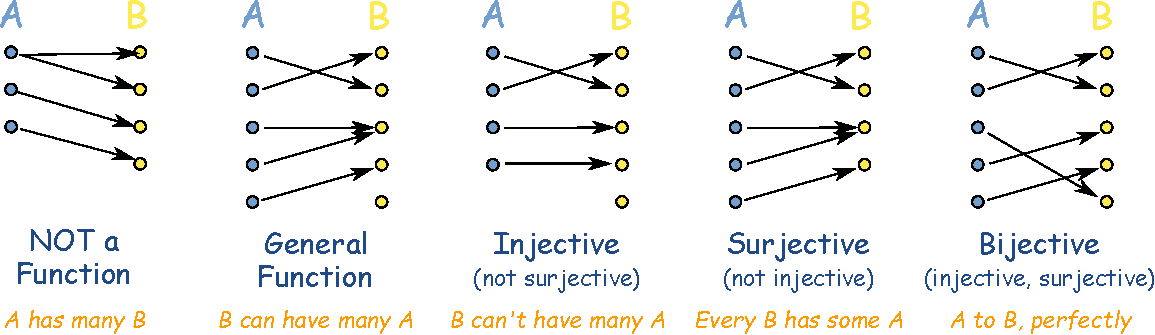
\includegraphics[width=0.7\linewidth]{pic/function-mapping.pdf}
        \caption{function-mapping}
        \label{fig:function-mapping}
    \end{figure}
    \mybox{
        injective ``one-to-one'' \\
        surjective ``onto'' \\
        bijective both injective and surjective. \\
        my question: what is ``into''?
    }

    If $E \subset B$, $f^{-1}(E)$ denotes the set of all $x \in A$ such that $f(x)\in E$. We call $f^{-1}(E)$ the \myKeywordblue{inverse image} of $E$ under $f$. If $y \in B$, $f^{-1}(y)$ is the set of all $x \in A$ such that $f(x) =y$. If, for each $y\in B$, $f^{-1}(y)$ consists of at most one element of $A$, then $f$ is said to be a 1-1 (\myKeywordblue{one-to-one}) mapping of $A$ into $B$. This may also be expressed as follows: $f$ is a 1-1 mapping of $A$ into $B$ provided that $f(x_1) \neq f(x_2)$ whenever $x_1 \neq x_2$, $x_1 \in A$, $x_2 \in A$.

    (The notation $x_1 \neq x_2$, means that $x_1$ and $x_2$ are distinct elements; otherwise we write $x_1 = x_2$.)
\end{mydef}

\begin{mydef}
    \label{mydef:2.3}
    If there exists a 1-1 mapping of $A$ \myKeywordblue{onto} $B$, we say that $A$ and $B$ can be putin 1-1 correspondence, or that $A$ and $B$ have the same cardinal number, or, briefly, that $A$ and $B$ are equivalent, and we write $A\sim B$. This relation
    clearly has the following properties :

    It is reflexive: $A\sim A$.

    It is symmetric: If $A\sim B$, then $B\sim A$.

    It is transitive: If $A\sim B$ and $B\sim C$, then $A\sim C$.

    Any relation with these three properties is called an equivalence relation.
\end{mydef}
\mybox{等价关系:
    reflexive   自反性,
    symmetric   对称性,
    transitive  传递性.

    集合等势是一种等价关系, 其满足自反性, 对称性, 传递性.}

\begin{mydef}
    \label{mydef:2.4}
    $\forall n\in \mathbb{N}^+$, $J_n = \{1,2,...,n\}$, $J = \{1,2,...,n,...\}$, (set consisting of all positive integers).

    $A$ is finite, $A\sim J_n$ for some n,

    $A = \varnothing$. empty set is also considered to be finite.

    $A$ is infinite, $A$ is not finite.

    $A$ is countable, $A \sim J$

    $A$ is uncountable. $A$ is neither finite nor countable.

    countable set and finite set are called at most countable.
\end{mydef}

\mybox{
    \begin{equation*}
        \left\{
        \begin{array}{lll}
            finite   & A\sim J_n \\
            infinite & \left\{
            \begin{array}{ll}
                countable   & A\sim J \\
                uncountable &         \\
            \end{array}
            \right.
        \end{array}
        \right.
    \end{equation*}
    % todo 添加tikz注释
}

countable sets, enumerable, denumerable.

$A, B \in$ finite set\\
$A\sim B$ $\Longleftrightarrow$ $A, B$ contains same number of elements

$A, B \in$ infinite set\\
same number or elements? vague\\
1-1 correspondence. retains its clarity.

\begin{newexample}
    $f:J\rightarrow A$
    \begin{equation*}
        f(n) = \left\{
        \begin{array}{ll}
            \cfrac{n}{2}    & (n \text{  even}) \\
            -\cfrac{n-1}{2} & (n \text{  odd})
        \end{array}
        \right.
    \end{equation*}
\end{newexample}
\mybox{$f(n)=(-1)^n\left\lfloor \cfrac{n}{2} \right\rfloor $}

\begin{myremark}
    a finite set cannot be equivalent to one of its proper subsets, but it's possible for infinite sets.
\end{myremark}

$J = 1,2,3,4,...$, $A = 0,1,-1,2,-2,...$,$J, A$are infinite sets, $J \subset A$.\\
but there exist a function $f:J\rightarrow A$, $J \sim A$

\begin{mydef}
    \label{mydef:2.7}
    $f(x)$, $x\in J = \mathbb{N}^+$.\\
    $\{x_n\}$, $x_1,x_2,x_3,...$\\
    $x_n$, terms of the sequence.\\
    $\forall n\in J$, $x_n\in A$, $\{x_n\}$ is a sequence in $A$, or a sequence of elements of $A$.
\end{mydef}

every countable set is range of a sequence of distinct terms.
the elements of any countable set can be ``arranged in a sequence''.
replace $J(\mathbb{N}^+)$ by $\mathbb{N} = \{x|, x\in Z,x \geq 0\}$, start with $0$ rather than $1$.

\begin{thm}
    \label{thm:2.8}
    Every infinite subset of a countable set $A$ is countable
\end{thm}

$E\subset A$. $E$ is infinite.
To prove $E$ is countable, we need a 1-1 correspondation of $J$ to $E$, $f:J\rightarrow E$.
\mybox{
    my first guess is $A$ is a countable set, $A\sim J$ (by def).
    $\exists$ 1-1 mapping $g:$ $J$ onto $A$.
    $x\in J$, $g(x)\in A$.
    $E\subset A$, $\exists  g(x)\in E$.
    $g(x_i)\in E$, $x_i\in J$, $g:J\rightarrow E$.\\
    再证 $x_i$ 不是有限的. $E$ is infinite, there exist infinite $g(x_i)\in E$. $\because g$ is a 1-1 mapping, $\{x_i\}$ is infinite. $\therefore J\sim E$.
}

\begin{proof}
    Suppose $E\subset A$, $E$ is infinite.
    arrange the elements $x$ of $A$ in a sequence $\{x_n\}$ of a distinct elements. Construct a sequence $n_k$ as follows.\\
    Let $n_1$ be the smallest positive int, s.t. $x_{n_1}\in E$.
    Having chosen $n_1,...n_{k-1}$,$(k=2,3,...)$, let $n_k$ be the smallest integer greater than $n_{k-1}$, s.t. $x_{n_k} \in E$.\\
    Putting $f(k) = x_{n_k}$, $f:J\rightarrow E$ is a 1-1 mapping.
\end{proof}

Countable sets represent the ``smallest'' infinity.

No uncountable set ca be a subset of a countable set.

\mybox{
    rudin 这里尝试区分实无穷与浅无穷,
    使用集合的势来说明更为具体, 全体整数组成的集合为 ``最小'' 的无穷大,
    其势为$\aleph_0$, 康托尔使用一一对应关系作为无穷集合之间的等价关系.
}

\begin{mydef}
    \label{mydef:2.9}
    $\forall \alpha\in A$, $E_\alpha \subset \Omega$, $\{E_\alpha\}$ debites elements of $E_\alpha$.
    collection of sets (or family of sets)
    \mybox{sets of sets sounds strange}
    union
    \begin{equation}
        \label{eq:2.1}
        S = \bigcup_{\alpha\in A} E_\alpha
    \end{equation}
    if $A$ consists of the integers $1,2,...,n$.
    \begin{equation}
        \label{eq:2.2}
        S = \bigcup_{m=1}^n E_m
    \end{equation}
    \begin{equation}
        \label{eq:2.3}
        S = E_1 \bigcup E_2 \bigcup \cdots \bigcup E_n.
    \end{equation}
    if $A$ is the set of all positive integers.
    \begin{equation}
        \label{eq:2.4}
        S = \bigcup_{m=1}^{\infty} E_m.
    \end{equation}
    intersection
    \begin{equation}
        \label{eq:2.5}
        P = \bigcap_{\alpha\in A} E_\alpha
    \end{equation}
    \begin{equation}
        \label{eq:2.6}
        S = \bigcap_{m=1}^n E_m = E_1 \cap E_2 \cap \cdots \cap E_n.
    \end{equation}
    \begin{equation}
        \label{eq:2.7}
        S = \bigcap_{m=1}^{\infty} E_m.
    \end{equation}

    $A$ and $B$ intersect if $A\bigcap B$ is not empty, otherwise they are disjoint.
\end{mydef}

\begin{newexample}
    % some example of set relation
    \begin{asparaenum}[(a)]
        \item Suppose $E_1$ consists of $1,2,3$ and
        $E_2$ consists of $2,3,4$.
        Then $E_1 \cup E_2$ consists of $1,2,3,4$,
        whereas $E_1 \cap E_2$ consists of $2,3$.
        \item Let $A$ be the set of real number $x$ such that $0< x\leq 1$.
        For every $x \in A$, let $E_x$ be the set of real numbers $y$ such that $0 < y < x$. Then
        \begin{asparaenum}[(i)]
            \item \[E_y \subset E_x \text{ if and only if } 0 < x \leq z \leq 1;\]
            \item \[\bigcup_{x\in A}E_x = E_1;\]
            \item \[\bigcap_{x\in A}E_x \text{ is empty};\]
        \end{asparaenum}
        (i) and (ii) are clear.
        To prove (iii), we note that for every $y>0$, $y \not\in E_x$ if $x < y$.
        Hence $y \not\in \cap_{x\in A}E_x$.
    \end{asparaenum}
\end{newexample}

\begin{myremark}
    Many properties of unions and intersections are quite similar to those of sums and products; in fact, the words sum and product were sometimes used in this connection, and the symbols $\sum$ and $\prod$ were written in place of $\bigcup$ and $\bigcap$.
\end{myremark}

The commutative and associative laws are trivial:
\begin{align}
    A \cup B                     & = B \cup A;                                   &
    A \cap B                     & = B \cap A \label{eq:2.8}                       \\
    \left(A \cup B\right) \cup C & = A \cup \left(B \cup C\right);               &
    \left(A \cap B\right) \cap C & = A \cap \left(B \cap C\right);\label{eq:2.9}
\end{align}

Thus the omission of parentheses in \ref{eq:2.3} and \ref{eq:2.6} is justified.

The distributive law also holds:
\begin{equation}
    \label{eq:2.10}
    A \cap \left( B \cup C\right) =
    \left(A \cap B\right) \cup \left(A \cap C\right).
\end{equation}
To prove this, let the left and right members of \ref{eq:2.10} be denoted by $E$ and $F$, respectively.

Suppose $x \in E$. Then $x \in A$ and $x \in B \cup C$, that is, $x \in B$ or$ x \in C$ (possibly both). Hence $x \in A\cap B$ or $x \in A\cap C$, so that $x \in F$. Thus $E \subset F$.

Next, suppose $x \in F$. Then $x \in A\cap B$ or $x \in A\cap C$. That is, $x \in A$, and $x \in B\cup C$. Hence $x \in A\cap \left(B \cup C\right)$, so that $F \subset E$.

It follows that $E = F$.

We list a few more relations which are easily verified:

\begin{align}
    A \subset A \cup B, \label{eq:2.11} \\
    A \cap B \subset B, \label{eq:2.12}
\end{align}

If $0$ denotes the empty set, then
\begin{equation}
    \begin{array}{cc}
        A \cup 0 = A, & A \cap 0 = 0.
    \end{array}
\end{equation}
If $A \subset B$, then
\begin{equation}
    \begin{array}{cc}
        A \cup B = B, & A \cap B = A.
    \end{array}
\end{equation}

\mybox{现在一般使用 $\varnothing$ 指代空集}


\begin{thm}
    \label{thm:2.12}
    Let $\{E_n\}, n=1,2,3,...,$ be a sequence of countable sets, and put
    \begin{equation}
        \label{eq:2.15}
        S = \bigcup_{n=1}^{\infty} E_n.
    \end{equation}
    Then S is countable.
\end{thm}
\mybox{
    将 $E_n$ 按顺序排成一张表格, 按反对角线重新排列成新的序列,
    得到 $T$, $S\sim T$.
    $S$ is at most countable.
    同时存在无限集合(infinite set) $E_1$, $E_1 \subset S$,
    $S$ is countable.
}

\begin{proof}
    Let every set $E_n$ be arranged in a sequence $\sequence{x_{nk}}$,
    $k = 1,2,3,\dots$,
    and consider the infinite array
    \begin{equation}
        \label{eq:2.16}
        \begin{array}{ccccc}
            x_{11} & x_{12} & x_{13} & x_{14} & \cdots \\
            x_{21} & x_{22} & x_{23} & x_{24} & \cdots \\
            x_{31} & x_{32} & x_{33} & x_{34} & \cdots \\
            x_{41} & x_{42} & x_{43} & x_{44} & \cdots \\
            \cdots & \cdots & \cdots & \cdots & \cdots \\
        \end{array}
    \end{equation}
    in which the elements of $E_n$ form the $n$th row.
    The array contains all elements of $S$.
    As indicated by the arrows,
    these elements can be arranged in a sequence
    \begin{equation}
        \label{eq:2.17}
        x_{11};
        x_{21}, x_{12};
        x_{31}, x_{22}, x_{13};
        x_{41}, x_{32}, x_{23}, x_{14};
        \cdots
    \end{equation}

    If any two of the sets En have elements in common,
    these will appear more than once in (\ref{eq:2.17}).
    Hence there is a subset $T$ of the set of all positive integers
    such that $S \sim T$,
    which shows that $S$ is at most countable (Theorem \ref{thm:2.8}).
    Since $E_1 \subset S$, and $E_1$ is infinite,
    $S$ is infinite, and thus countable.
\end{proof}

\begin{myCorollary*}
    Suppose $A$ is at most countable, and, for every $\alpha \in A, B$, is at most countable. Put
    \begin{equation*}
        T = \bigcup_{\alpha\in A} B_\alpha.
    \end{equation*}
    Then T is at most countable.
\end{myCorollary*}

For $T$ is equivalent to a subset of \ref{eq:2.15}.

\begin{thm}
    \label{thm:2.13}
    Theorem Let $A$ be a countable set, and let $B_n$ be the set of all $n$-tuples $(a_1, ...,a_n)$, where $a_k \in  A (k=1,...,n)$, and the elements $a_1, ...,a_n$ need not be distinct. Then $B_n$ is countable.
\end{thm}

\begin{proof}
    That $B_1$ is countable is evident, since $B_1 = A$.
    Suppose $B_{n-1}$ is countable $(n = 2, 3, 4, ... )$.
    The elements of $B_n$ are of the from
    \begin{equation}
        \label{eq:2.18}
        (b,a)
        \quad
        (b \in B_{n-1},a \in A).
    \end{equation}
    For every fixed $b$, the set of pairs $(b, a)$ is equivalent to $A$, and hence countable.
    Thus $B_n$ is the union of a countable set of countable sets.
    By Theorem \ref{thm:2.12}, $B_n$ is countable.
    The theorem follows by induction.
\end{proof}

\begin{myCorollary*}
    The set of all rational numbers is countable.
\end{myCorollary*}

\begin{proof}
    We apply Theorem \ref{thm:2.13},
    with $n = 2$, noting that every rational $r$ is of the form $b / a$,
    where $a$ and $b$ are integers.
    The set of pairs $(a, b)$,
    and therefore the set of fractions $b / a$, is countable.
\end{proof}

In fact, even the set of all algebraic numbers is countable (see Exercise \ref{ex:1.2}).

That not all infinite sets are, however, countable, is shown by the next
theorem.

\begin{thm}
    \label{thm:2.14}
    Theorem Let $A$ be the set of all sequences whose elements are the digits $0$ and $1$.
    This set $A$ is uncountable.
\end{thm}

The elements of $A$ are sequences like $1, 0, 0, 1, 0, 1, 1, 1, ... .$

\begin{proof}
    Let $E$ be a countable subset of $A$,
    and let $E$ consist of the sequences $s_1, s_2 , s_3 , ...$.
    We construct a sequences as follows.
    If the $n$th digit in $s_n$ is $1$,
    we let the $n$th digit of $s$ be $0$, and vice versa.
    Then the sequence $s$ differs from every member of $E$ in at least one place; hence $s \not\in E$.
    But clearly $s \in A$, so that $E$ is a proper subset of $A$.

    We have shown that
    every countable subset of $A$ is a proper subset of $A$.
    It follows that $A$ is uncountable
    (for otherwise $A$ would be a proper subset of $A$, which is absurd).
\end{proof}

The idea of the above proof was first used by Cantor,
and is called Cantor's diagonal process;
for, if the sequences $s_1, s_2 , s_3 ,\dots$ are placed in an array like (\ref{eq:2.16}),
it is the elements on the diagonal which are involved in the construction of the new sequence.

Readers who are familiar with the binary representation of the real numbers (base 2 instead of 10) will notice that
Theorem \ref{thm:2.14} implies that the set of all real numbers is uncountable.
We shall give a second proof of this fact in Theorem \ref{thm:2.43}.
\section{Metric space}
\mybox{metirc space 度量空间}
\begin{mydef}\label{mydef:2.15}
    set $X$ metric space $p\in X$, $p$ point.

    $\forall p,q \in X$ associate a real number $d(p,q)$ (distance)
    \begin{enumerate}[a.]
        \item $d(p,q) > 0$ if $p \neq q$; $d(p,p)=0$,
        \item $d(p,q) = d(q,p)$.
        \item $d(p,q) \leq d(p,r) + d(r,q)$, $\forall r\in X$
    \end{enumerate}
\end{mydef}
\mybox{对称性, 正定性, 三角不等式. }

\begin{newexample}
    the distance of the euclidean space $\R^k$ is defined by
    \begin{equation}\label{eq:2.19}
        d(\mathbf{x}, \mathbf{y}) = |\mathbf{x} - \mathbf{y}|
        \qquad (\mathbf{x}, \mathbf{y}\in \R^k)
    \end{equation}
\end{newexample}

It's important to observe that every subset $Y$ of metric space $X$ is a metric space in its own right, with the same distance function. For it is clear that if conditions (a) to (c) of Definition \ref{mydef:2.15} hold for $p, q, r \in X$, they also hold if we restrict $p, q, r$ to lie in $Y$.

Thus every subset of a euclidean space is a metric space. Other examples
are the spaces $l(K)$ and $L^2 (\mu)$, 
which are discussed in Chaps. 7 and 11, respectively.

% \mybox{
%     使用 mathescr 命令输入英文花体字(报错,改用 mathcal)
%     $\mathscr{l} (K)$ and $\mathscr{l}^2 (\mu)$

%     Ralph Smith’s Formal Script Font (rsfs): Use the “mathrsfs” package.
%     usepackage{mathrsfs}
    
%     $\mathscr{ABCDEFGHIJKLMNOPQRSTUVWXYZ}$

%     % $\mathscr{abcdefghijklmnopqrstuvwxyz}$

%     % % $\mathrsfs{abcdefghijklmnopqrstuvwxyz}$
%     % $\mathcal{abcdefghijklmnopqrstuvwxyz}$ % 小写字母打印出来是乱码
%     $\mathcal{ABCDEFGHIJKLMNOPQRSTUVWXYZ}$

%     $\mathfrak{ABCDEFGHIJKLMNOPQRSTUVWXYZ}$
% }

\begin{mydef}
    \label{mydef:2.17}
By the \myKeywordblue{segment} $(a, b)$ we mean the set of all real numbers $x$
such that $a < x <b$.

By the \myKeywordblue{interval} $[a. b]$ we mean the set of all real numbers $x$ such that $a \leq x \leq b$

Occasionally we shall also encounter ``half-open intervals'' $[a, b)$ and $(a, b]$; the first consists of all $x$ such that $a \leq x < b$, the second of all $x$ such that $a < x \leq b$
\end{mydef}

If $a_i <b_i$ for $i=1,...,k$, the set of all points $\mathbf{x} =(x_1, ..., x_k)$ in $\R^k$ whose coordinates satisfy the inequalities $a_i \leq x_i \leq _i (1 \leq i \leq k)$ is called a \myKeywordblue{$k$-cell}.\\
Thus a $1$-cell is an interval, a $2$-cell is a rectangle, etc.

If $\mathbf{x}\in \R^k$ and $r > 0$. the \myKeywordblue{open (or closed) ball} $B$ with center at $\mathbf{x}$ and radius $r$ is defined to be the set of all $\mathbf{y} \in \R^k$ such that $|\mathbf{y} - \mathbf{x}| <r$ (or $|\mathbf{y} - \mathbf{x}| \leq r$).

We call a set $E \subset \R^k$ \myKeywordblue{convex} if

\begin{equation*}
    \lambda\mathbf{x} + (1 - \lambda)\mathbf{y} \in E
\end{equation*}

whenever $\mathbf{x} \in E$, $\mathbf{y} \in E$, and $0 < \lambda < 1$.

For example, \myKeywordblue{balls are convex}. For if |y -x| <r, |z-x| <r, and
$0 < \lambda <1$, we have
\begin{align*}
    |\lambda \mathbf{y} + (1-\lambda) \mathbf{z} - \mathbf{x}|
    & = |\lambda (\mathbf{y} - \mathbf{x}) + (1 - \lambda)(\mathbf{z} - \mathbf{x})\\
    & \leq \lambda |\mathbf{y} - \mathbf{x}| + (1 - \lambda)|\mathbf{z} - \mathbf{x}| < \lambda r + (1 - \lambda)r\\
    & = r.
\end{align*}

The same proof applies to closed balls. It is also easy to see that $k$-cells are convex.
% 32 PRINCIPLES OF MATHEMATICAL ANALYSIS

\mybox{这里给出了 开区间, 闭区间, 半开区间以及凸集 convex 的定义

凸性 Jensen 不等式.
}

\begin{mydef}\label{mydef:2.18}
    Definition Let $X$ be a metric space. All points and sets mentioned below are understood to be elements and subsets of $X$.
    \begin{enumerate}[(a)]
        \item A \myKeywordblue{neighborhood} of $p$ is a set $N_r(p)$ consisting of all $q$ such that $d(p, q) < r$,for some $r > 0$. The number $r$ is called the \myKeywordblue{radius} of $N_r(p)$.
        \item A point $p$ is a \myKeywordblue{limit point} of the set $E$ if \myKeywordblue{every} neighborhood of $p$ contains a point $q \neq p$ such that $q \in E$.
        \item If $p \in E$ and $p$ is not a limit point of $E$, then $p$ is called an \myKeywordblue{isolated point} of $E$.
        \item $E$ is \myKeywordblue{closed} if every limit point of $E$ is a point of $E$.
        \item A point $p$ is an \myKeywordblue{interior} point of $E$ if there is a neighborhood $N$ of $p$ such that $N \subset E$.
        \item $E$ is \myKeywordblue{open} if every point of $E$ is an interior point of $E$.
        \item The \myKeywordblue{complement} of $E$ (denoted by $E^c$)is the set of all points $p \in X$ such that $p \not\in E$.
        \item $E$ is \myKeywordblue{perfect} if $E$ is closed and if every point of $E$ is a limit point of $E$.
        \item $E$ is \myKeywordblue{bounded} if there is a real number $M$ and a point $q \in X$ such that $d(p,q)< M$ for all $p \in E$.
        \item $E$ is \myKeywordblue{dense} in $X$ if every point of $X$ is a limit point of $E$, or a point of $E$ (or both).
    \end{enumerate}
\end{mydef}

Let us note that in $\R^1$ neighborhoods are segments, whereas in $\R^2$ neighborhoods are interiors of circles.

\mybox{
    neighbhoods 邻域, \\
    limit point 极限点, 
    isolated point 孤立点, 
    interior point 内点. \\
    closed set 闭集, open set 开集, closure set 补集.\\
    perfect set 完全集, complete set 完备集, 
    dense 稠密 (有理数集 $\Q $ 是稠密的, 与之对应 实数集 $\R$ 是连续的.)

    这里闭集的定义是包含所有极限点的集合, 而开集的定义是所有点均为内点. 乍一看这两个定义是不相关的, 但后续会证明开集的补集是闭集, 闭集的补集是开集. 这种定义与过去的定义不冲突, 并且更容易理解空集既是开集也是闭集.
}

\begin{thm}
    \label{thm:2.19}
    Every neighborhood is an open set.
\end{thm}
\begin{proof}
    Consider a neighborhood $E = N_r(p)$, 
    and let $q$ be any point of $E$.
    Then there is a positive real number $h$ such that
    \begin{equation*}
        d(p, q) = r - h.
    \end{equation*}
    For all points $s$ such that $d(q, s) < h$, we have then
    \begin{equation*}
        d(p, s) \leq d(p, q) + d(q, s) < r - h + h = r,
    \end{equation*}
    so that $s \in E$. 
    Thus $q$ is an interior point of $E$.
\end{proof}

\begin{thm}
    \label{thm:2.20}
    If $p$ is a limit point of a set $E$, then every neighborhood of $p$ contains infinitely many points of $E$.
\end{thm}

\begin{proof}
    Suppose there is a neighborhood $N$ of $p$ 
    which contains only a finite number of points of $E$. 
    Let $q_1, ... , q_n$ be those points of $N \cap E$,
    which are distinct from $p$, and put
    \begin{equation*}
        r = \min_{1 \leq m \leq n} d(p, q_m)
    \end{equation*}
    [we use this notation to denote the smallest of the numbers 
    $d(p, q_1), ..., d(p, q_n)$]. 
    The minimum of a finite set of positive numbers is clearly positive, 
    so that $r > 0$.

    The neighborhood $N_r(p)$ contains no point $q$ of $E$ such that $q \neq p$,
    so that $p$ is not a limit point of $E$. 
    This contradiction establishes the theorem.
\end{proof}

\begin{myCorollary*}
    A finite point set has no limit points.
\end{myCorollary*}

\begin{newexample}
    \label{newexample:2.21}
    Let us consider the following subsets of $\R^{2}$:
    \begin{enumerate}[(a)]
        \item The set of all complex $z$ such that $|z| < 1$.
        \item The set of all complex $z$ such that $|z| \leq 1$.
        \item A nonempty finite set.
        \item The set of all integers.
        \item The set consisting of the numbers $1/n(n=1,2,3,...)$. Let us note that this set $E$ has a limit point (namely, $z =0$) but that no point of $E$ is a limit point of $E$; we wish to stress the difference between having a limit point and containing one.
        \item The set of all complex numbers (that is, $\R^{2}$).
        \item The segment $(a,b)$.
    \end{enumerate}
\end{newexample}

Let us note that (d),(e),(g)can be regarded also as subsets of $\R^{1}$.
Some properties of these sets are tabulated below:

\begin{center}
    \begin{tabular}{lcccc}
        & Closed & Open & Perfect & Bounded \\
    (a) & No     & Yes  & No      & Yes     \\
    (b) & Yes    & No   & Yes     & Yes     \\
    (c) & Yes    & No   & No      & Yes     \\
    (d) & Yes    & No   & No      & No      \\
    (e) & No     & No   & No      & Yes     \\
    (f) & Yes    & Yes  & Yes     & No      \\
    (g) & No     &      & No      & Yes    
    \end{tabular}
\end{center}

In (g), we left the second entry blank. 
The reason is that the segment $(a,b)$ is not open 
if we regard it as a subset of $\R^2$, 
but it is an open subset of $\R^1$.

\mybox{根据定义, 复数集既是闭集又是开集...}

\begin{thm}
    \label{thm:2.22}
    Let $\{E_\alpha\}$ be a (finite or infinite) collection of sets $E_\alpha$. Then
    \begin{equation}
        \label{eq:2.20}
        \left(\bigcup_{\alpha} E_{\alpha} \right)^c = \bigcap_{\alpha}( E_{\alpha}^c )
    \end{equation}
\end{thm}

\begin{proof}
    Let $A$ and $B$ be the left and right members of (\ref{eq:2.20}). 
    If $x \in A$, then $X \not\in \cup_\alpha E_\alpha$, 
    hence $x \not\in E_\alpha$ for any $\alpha$, 
    hence $x \in E_\alpha^c$ for every $\alpha$, 
    so that $x \in \cap E_\alpha^c$.
    Thus $A \subset B$.

    Conversely, if $x \in B$, then $x \in E_\alpha^c$ for every $\alpha$,
    hence $x \not\in E_\alpha$ for any $\alpha$,
    hence $x \not\in \cup_\alpha E_\alpha$, 
    so that $x \in (\cup_\alpha E_\alpha)^c$. 
    Thus $B \subset A$.

    It follows that $A = B$.
\end{proof}

\begin{thm}
    \label{thm:2.23}
    A set $E$ is open if and only if its complement is closed.
\end{thm}

\begin{proof}
    % Proof 
    First, suppose $E^c$ is closed. Choose $x \in E$. Then $x \not\in E^c$, and $x$ is not a limit point of $E^c$. Hence there exists a neighborhood $N$ of $x$ such that $E^c \cap N$ is empty, that is, $N \subset E$. Thus $x$ is an interior point of $E$, and $E$ is open.
    
    Next, suppose $E$ is open. Let $x$ be a limit point of $E^c$. Then every neighborhood of $x$ contains a point of $E^c$, so that $x$ is not an interior point of $E$. Since $E$ is open, this means that $x \in E^c$. It follows that $E$ is closed.
\end{proof}

\begin{myCorollary*}
    A set $F$ is closed if and only if its complement is open.
\end{myCorollary*}

\mybox{这里使用新的定义得到的开集与闭集保持了原有的性质: 开集的补集是闭集, 闭集的补集是开集}

\begin{thm}
    \label{thm:2.24}
    \begin{enumerate}[(a)]
        \item For any collection $\{G_\alpha\}$ of open sets,  $\cup_\alpha G_\alpha$ is open.
        \item For any collection $\{F_\alpha\}$ of closed sets, $\cap_\alpha F_\alpha$ is closed.
        \item For any finite collection $G_1, ..., G_n$ of open sets, $\cap_{i=1}^n G_i$ is open.
        \item For any finite collection $F_1, ..., F_n$ of closed sets, $\cup_{i=1}^n F_i$ is closed.
    \end{enumerate}
\end{thm}

\begin{proof}
    Put 

    By Theorem \ref{thm:2.22}
    \begin{equation}
        \label{eq:2.21}
        \left( \bigcap_\alpha F_\alpha \right)^c = 
        \bigcup_\alpha \left( F_\alpha^c \right),
    \end{equation}
\end{proof}

\mybox{
    无限开集的并仍是开集, 有限开集的交仍是开集\\
    无限闭集的交仍是闭集, 有限闭集的并仍是闭集\\
    下面给出一个反例
}

\begin{newexample}
    In parts (c)and (d) of the preceding theorem, the finiteness of the collections is essential.
    \begin{equation*}
        G_n = \left(-\frac{1}{n}, \frac{1}{n} \; (n=1,2,3,\dots). \right)
    \end{equation*}
    $G = \cap_{n=1}^\infty G_n$
    Then $G$ consists of a single point (namely, $x = 0$) and is therefore not an open subset of $\R$.
    
    Thus the intersection of an infinite collection of open sets need not be open. Similarly, the union of an infinite collection of closed sets need not be closed.
\end{newexample}

\begin{mydef}
    \label{mydef:2.26}
    If $X$ is a metric space, if $E \subset X$, and if $E'$ denotes the set of all limit points of $E$ in $X$, then the \myKeywordblue{closure} of $E$ is the set $\overline{E}=E \cup E'$.
\end{mydef} 
\mybox{
    Closure 闭包

The term "closure" has various meanings in mathematics.

The topological closure of a subset $A$ of a topological space $X$ is the smallest closed subset of $X$ containing $A$.

If $R$ is a binary relation on some set $A$, then $R$ has reflexive, symmetric and transitive closures, each of which is the smallest relation on $A$, with the indicated property, containing $R$. Consequently, given any relation $R$ on any set $A$, there is always a smallest equivalence relation on $A$ containing $R$.

For some arbitrary property $P$ of relations, the relation $R$ need not have a $P$-closure, i.e., there need not be a smallest relation on $A$ with the property $P$, and containing $R$. 
For example, it often happens that a relation does not have an antisymmetric closure.

In algebra, the algebraic closure of a field $F$ is a field $\bar{F}$ which can be said to be obtained from $F$ by adjoining all elements algebraic over $F$.
}

\begin{thm}
    \label{thm:2.27}
    If $X$ is a metric space and $E \subset X$, then
    \begin{enumerate}[(a)]
        \item $E$ is closed,
        \item $E = \overline{E}$ if and only if $E$ is closed,
        \item $E \subset F$ for every closed set $F \subset X$ such that $E \subset F$.
    \end{enumerate}
\end{thm}
By (a) and (c), $E$ 1s the smallest closed subset of $X$ that contains $E$.
\begin{proof}
    \begin{enumerate}[(a)]
        \item If $p \in X$ and $p \not\in \overline{E}$ then $p$ is neither a point of $E$ nor a limit point of $E$. Hence $p$ has a neighborhood which does not intersect $E$. The complement of $E$ is therefore open. Hence $E$ is closed.
        \item If $E = \overline{E}$, (a) implies that $E$ is closed. If $E$is closed, then $E' \subset E$ [by Definitions \ref{mydef:2.18}(d) and \ref{mydef:2.26}], hence $\overline{E} = E$.
        \item If $F$ is closed and $F \supset E$, then $F \supset F'$, hence $F \supset E'$. Thus $F \supset \overline{E}$.
    \end{enumerate}
\end{proof}


\begin{thm}
    \label{thm:2.28}
    Let $E$ be a nonempty set of real numbers which is bounded above.     Let $y = \sup E$. Then $y \in \overline{E}$. Hence $y \in E$ if $E$ is closed.
\end{thm}
Compare this with the examples in Sec. 1.9.
\begin{proof}
    If $y \in E$ then $y \in \overline{E}$. 
    Assume $y \not\in E$. 
    For every $h > 0$ there exists then a point $x \in E$ 
    such that $y - h < x < y$, 
    for otherwise $y - h$ would be an upper bound of $E$. 
    Thus $y$ is a limit point of $E$. Hence $y \in \overline{E}$.
\end{proof}

\begin{myremark}
    \label{myremark:2.29}
    Suppose $E \subset Y \subset X$, where $X$ is a metric space. To say that $E$ is an open subset of $X$ means that to each point $p \in E$ there is associated a positive number $r$ such that the conditions $d(p,q) < r$ , $g \in X$ imply that $q \in E$. But we have already observed (Sec. 2.16) that $Y$ is also a metric space, so that our definitions may equally well be made within $Y$. To be quite explicit, let us say that 
    
    $E$ is \myKeywordblue{open relative to $Y$} if to each $p \in E$ there is associated an $r > 0$ such that $q \in E$ whenever $d(p,q) <r$ and $g \in Y$. 
    
    Example 2.21(g) showed that a set may be open relative to $Y$ without being an open subset of $X$. However, there is a simple relation between these concepts, which we now state.
\end{myremark}
\mybox{open relative to $Y$ 关于Y是开的} 

\begin{thm}
    \label{thm:2.30}
    Suppose $Y \subset X$. A subset $E$ of $Y$ is open relative to $Y$ if and only if $E = Y \cap G$ for some open subset $G$ of $X$.
\end{thm}
\begin{proof}
    Suppose $E$ is open relative to $Y$. 
    To each $p \in E$ there is a positive number $r_P$ 
    such that the conditions $d(p, q) < r_P$, 
    $q \in Y$ imply that $q \in E$. 
    Let $V_P$ be the set of all $q \in X$ 
    such that $d(p, q) < r_P$, and define
    \begin{equation*}
        G = \bigcup_{p \in E} V_P.
    \end{equation*}
    Then $G$ is an open subset of $X$, by Theorems \ref{thm:2.19} and \ref{thm:2.24}. 

    Since $p \in V_P$ for all $p \in E$, 
    it is clear that $E \subset G \cap Y$.
    
    By our choice of $V_P$, 
    we have $V_P \cap Y \subset E$ for every $p \in E$, 
    so that $G \cap Y \subset E$. 
    Thus $E = G \cap Y$, and one half of the theorem is proved.
    
    Conversely, if $G$ is open in $X$ and $E = G \cap Y$, 
    every $p \in E$ has a neighborhood $V_P \subset G$. 
    Then $V_P \cap Y \subset E$, 
    so that $E$ is open relative to $Y$.
\end{proof}
% chap02sec03
\section{Compact sets}

\mybox{

    Compact set 紧集

    \url{https://mathworld.wolfram.com/CompactSet.html}

    A subset $S$ of a topological space $X$ is compact if for every open cover of $S$ there exists a finite subcover of $S$.

    紧集的任何开覆盖都有有限子覆盖

    在 $\R^{n}$中, 下面三个条件等价: Theorem \ref{thm:2.41}
    有界闭 (bounded and closed);
    紧 (compact);
    列紧 (sequentially compact);
}

\begin{mydef}
    \label{mydef:2.31}
    By an \emph{open cover} of a set $E$ in a metric space $X$ we mean a collection $\sequence{G_{\alpha}}$ of open subsets of $X$ such that $E \subset \cup_{\alpha} G_{\alpha}$.
\end{mydef}

\begin{mydef}
    \label{mydef:2.32}
    A subset $K$ of a metric space $X$ is said to be \emph{compact} if every open cover of $K$ contains a \emph{finite} subcover.
\end{mydef}
\mybox{有限开覆盖定理. 紧集的介绍从开覆盖开始, 紧集的每个开覆盖包含一个有限子覆盖.}

More explicitly, the requirement is that if $\sequence{G_{\alpha}}$ is an open cover of $K$, then there are finitely many indices $\alpha_1, ..., \alpha_n$ such that
\begin{equation*}
    K \subset G_{\alpha_{1}} \cup \cdots \cup G_{\alpha_{n}}.
\end{equation*}

The notion of compactness is of great importance in analysis, especially
in connection with continuity (Chap. \ref{chap:04}).

It is clear that every finite set is compact. The existence of a large class of infinite compact sets in $\R^k$ will follow from Theorem 2.41.

We observed earlier (in Sec. 2.29) that if $E \subset Y \subset X$, then $E$ may be open relative to $Y$ without being open relative to $X$. The property of being open thus depends on the space in which $E$ is embedded. The same is true of the property of being closed.

Compactness, however, behaves better, as we shall now see. To formulate the next theorem, let us say, temporarily, that $K$ is compact relative to $X$ if the requirements of Definition 2.32 are met.
% BASIC TOPOLOGY 37

\begin{thm}
    \label{thm:2.33}
    Suppose $K \subset Y \subset X$. Then $K$ is compact relative to $X$ if and only if $K$ is compact relative to $Y$.
\end{thm}

By virtue of this theorem we are able, in many situations,
to regard compact sets as metric spaces in their own right,
without paying any attention to any embedding space.
In particular, although it makes little sense to talk of \emph{open} spaces,
or of \emph{closed} spaces
(every metric space $X$ is an open subset of itself,
and is a closed subset of itself),
it does make sense to talk of \emph{compact} metric spaces.

\begin{proof}
    % Proof 
    Suppose $K$ is compact relative to $X$, and let $\sequence{V_\alpha}$ be a collection of sets, open relative to $Y$, such that $K \subset \cup_\alpha V_\alpha$ theorem 2.30, there are sets $G_\alpha$, open relative to $X$, such that $V_\alpha = Y \cap G_\alpha$, for all $\alpha$; and since $K$ is compact relative to $X$, we have
    \begin{equation}\label{eq:2.22}
        K \subset G_{\alpha_{1}} \cup \cdots \cup G_{\alpha_{n}}.
    \end{equation}
    for some choice of finitely many indices $\alpha_1 ..., \alpha_n$. Since $K \subset Y$, \ref{eq:2.22} implies
    \begin{equation}\label{eq:2.23}
        K \subset V_{\alpha_{1}} \cup \cdots \cup V_{\alpha_{n}}.
    \end{equation}
    This proves that $K$ is compact relative to $Y$.

    Conversely, suppose $K$ is compact relative to $Y$, let $G_\alpha$ be a collection of open subsets of $X$ which covers $K$, and put $V_\alpha = Y \cap G_\alpha$. Then \ref{eq:2.23} will hold for some choice of $\alpha_1, ...,\alpha_n$; and since $V_\alpha = G_\alpha$, \ref{eq:2.23} implies \ref{eq:2.22}.

    This completes the proof.
\end{proof}

\begin{thm}
    \label{thm:2.34}
    Compact subsets of metric spaces are closed.
\end{thm}

\begin{proof}
    Let $K$ be a compact subset of a metric space $X$.
    We shall prove that the complement of $K$ is an open subset of $X$.

    Suppose $p \in X$, $p \not\in K$.
    If $q \in K$, let $V_q$ and $W_q$ be neighborhoods of $p$ and $q$,
    respectively, of radius less than $\tfrac{1}{2}d(p, q)$ [see Definition \ref{mydef:2.18}(a)].
    Since $K$ is compact, there are finitely many points $q_1, ..., q_n$ in $K$ such that
    \begin{equation*}
        K \subset
        W_{q_1} \cup \cdots \cup
        W_{q_n}.
    \end{equation*}

    If $V=V_{q_1} \cap \cdots \cap V_{q_1}$,
    then $V$ is a neighborhood of $p$ which does not intersect $W$.
    Hence $V \subset K^c$, so that $p$ is an interior point of $K^c$.
    The theorem follows.
\end{proof}

\begin{thm}
    \label{thm:2.35}
    Closed subsets of compact sets are compact.
\end{thm}
\mybox{紧集的闭子集仍是紧集}

\begin{proof}
    Suppose $F \subset K \subset X$,
    $F$ is closed (relative to $X$),
    and $K$ is compact.
    Let $\sequence{V_\alpha}$ be an open cover of $F$.
    If $F^c$ is adjoined to $\sequence{V_\alpha}$,
    we obtain an open cover $\Omega$ of $K$.
    Since $K$ is compact, there is a finite subcollection $\Phi$ of $\Omega$ which covers $K$, and hence $F$.
    If $F^c$ is a member of $\Phi$,
    we may remove it from $\Phi$ and still retain an open cover of $F$.
    We have thus shown that a finite subcollection of $\sequence{V_\alpha}$ covers $F$.
\end{proof}

\begin{myCorollary*}
    If $F$ is closed and $K$ is compact, then $F \cap K$ is compact.
\end{myCorollary*}

\begin{proof}
    Theorems \ref{thm:2.24}(b) and \ref{thm:2.34} show that $F \cap K$ is closed;
    since $F \cap K \subset K$,
    Theorem \ref{thm:2.35} shows that $F \cap K$ is compact.
\end{proof}

\begin{thm}
    \label{thm:2.36}
    % 2.36 Theorem
    If $\sequence{K_\alpha}$ is a collection of compact subsets of a metric space $X$
    such that the intersection of every finite subcollection of $\sequence{K_\alpha}$ is nonempty,
    then $\cap K_\alpha$ is nonempty.
\end{thm}

\begin{proof}
    Fix a member $K_1$ of $\sequence{K_\alpha}$ and put $G_\alpha = K^c_\alpha$.
    Assume that no point of $K_1$ belongs to every $K_\alpha$.
    Then the sets $G_\alpha$ form an open cover of $K_1$;
    and since $K_1$ is compact, there are finitely many indices $\alpha_1, ..., \alpha_n$ such that $K \subset G_{\alpha_1} \cup \cdots \cup G_{\alpha_n}$.
    But this means that
    \begin{equation*}
        K_1 \cap
        K_{\alpha_1} \cap
        \dots \cap
        K_{\alpha_n}
    \end{equation*}
    is empty, in contradiction to our hypothesis.
\end{proof}

\begin{myCorollary*}
    If $\sequence{K_\alpha}$ is a sequence of nonempty compact sets such that $K_n \supset K_{n+1} (n=1,2,3,...)$, then $\cap_1^\infty K_n$ is not empty.
\end{myCorollary*}

\begin{thm}
    \label{thm:2.37}
    If $E$ is an infinite subset of a compact set $K$,
    then $E$ has a limit point in $K$.
\end{thm}

\begin{proof}
    If no point of $K$ were a limit point of $E$,
    then each $q \in K$ would have a neighborhood $V_q$ which contains at most one point of $E$ (namely, $q$, if $q \in E$).
    It is clear that no finite subcollection of $\sequence{V_q}$ can cover $E$;
    and the same is true of $K$, since $E \subset K$. This contradicts the compactness of $K$.
\end{proof}

\begin{thm}
    \label{thm:2.38}
    If $\sequence{I_n}$ is a sequence of intervals in $\R^1$,
    such that $I_n \supset I_{n+1}, (n=1,2,3,...)$,
    then $\cap_1^\infty I_n$ is not empty.
\end{thm}

\begin{proof}
    If $I_n = [a_n, b_n]$, let $E$ be the set of all $a_n$.
    Then $E$ is nonempty and bounded above (by $b_1$).
    Let $x$ be the sup of $E$.
    If $m$ and $n$ are positive integers, then
    \begin{equation*}
        a_{n} \leq
        a_{m+n} \leq
        b_{m+n} \leq
        b_{n} .
    \end{equation*}
    so that $x \leq b_m$ for each $m$.
    Since it is obvious that $a_m \leq x$,
    we see that $x \in I_m$ for $m = 1, 2, 3, ...$.
\end{proof}

\begin{thm}
    \label{thm:2.39}
    Let $k$ be a positive integer.
    If ${I_n}$ is a sequence of $k$-cells such that $I_n \supset I_{n+1}, (n=1,2,3,...)$,
    then $\cap_1^\infty I_n$ is not empty.
\end{thm}

\begin{proof}
    Let $I_n$ consist of all points $\mathbf{x} = (x_1,...,x_k)$ such that
    \begin{equation*}
        a_{n, j} \leq
        x_j \leq
        b_{n, j}
        \quad
        (1 \leq j \leq k; n = 1,2,3,...),
    \end{equation*}
    and put $I_{n,j} = [a_{n,j}, b_{n,j}]$.
    For each $j$, the sequence $\sequence{I_{n,j}}$ satisfies the hypotheses of Theorem \ref{thm:2.38}.
    Hence there are real numbers $x_j^*(1 \leq j \leq k)$ such that
    \begin{equation*}
        a_{n,j}
        \leq x_j^* \leq
        b_{n,j}
        \quad
        (1 \leq j \leq k; n = 1, 2, 3, ... ).
    \end{equation*}
    Setting $\mathbf{x}* = (x_1^*, ... , x_k^*)$,
    we see that $\mathbf{x}^* \in I_n$ for $n = 1, 2, 3, ...$.
    The theorem follows.
\end{proof}

\begin{thm}
    \label{thm:2.40}
    Every $k$-cell is compact.
\end{thm}

\begin{proof}
    Let $I$ be a $k$-cell,
    consisting of all points $\mathbf{x} = (x_1, \dots, x_k)$
    such that $a_j \leq x_j \leq  b_j (1 \leq j \leq k)$.
    Put
    \begin{equation*}
        \delta =
        \left\sequence{ \sum_{1}^{k} (b_j - a_j)^2 \right}^{1/2}
    \end{equation*}
    Then $ \left| \mathbf{x-y} \right| \leq \delta$, if $x \in I, y \in I$.

    Suppose, to get a contradiction,
    that there exists an open cover $\sequence{G_\alpha}$ of $I$
    which contains no finite subcover of $I$.
    Put $c_j = (a_j + b_j)/2$.
    The intervals $[a_j , c_j]$ and $[c_j , b_j]$
    then determine $2^k$ $k$-cells $Q_i$ whose union is $I$.
    At least one of these sets $Q_i$, call it $I_1$,
    cannot be covered by any finite subcollection of $\sequence{G_\alpha}$
    (otherwise $I$ could be so covered).
    We next subdivide $I_1$ and continue the process.
    We obtain a sequence $\sequence{I_n}$ with the following properties:
    \begin{enumerate}[(a)]
        \item $I \supset I_1 \supset I_2 \supset I_3 \supset \dots$;
        \item $I_n$ is not covered by any finite subcollection of $\sequence{G_\alpha}$;
        \item if $\mathbf{x} \in I_n$ and $\mathbf{y} \in I_n$ , then $\left| \mathbf{x-y} \right| \leq 2^{-n}\delta$.
    \end{enumerate}

    By (a) and Theorem \ref{thm:2.39}, there is a point $\mathbf{x}^*$ which lies in every $I_n$.
    For some $\alpha$, $\mathbf{x}^* \in G_\alpha$.
    Since $G_\alpha$ is open, there exists $r > 0$ such that
    $\left| \mathbf{y-x}^* \right| < r$ implies that $\mathbf{y} \in G_\alpha$.
    If $n$ is so large that $2^{-n}\delta < r$
    (there is such an $n$, for otherwise $2^n \leq \delta/r$ for all positive integers $n$, which is absurd since $\R$ is archimedean),
    then (c) implies that $I_n \subset G_\alpha$, which contradicts (b).

    This completes the proof.
\end{proof}

The equivalence of (a) and (b) in the next theorem is known as the Heine-Borel theorem.

\begin{thm}
    \label{thm:2.41}
    If a set $E$ in $\R^k$ has one of the following three properties, then it has the other two:
    \begin{enumerate}[(a)]
        \item $E$ is closed and bounded.
        \item $E$ is compact.
        \item Every infinite subset of $E$ has a limit point in $E$.
    \end{enumerate}
\end{thm}

\mybox{
    在 $\R^{n}$中, 下面三个条件等价:
    有界闭 (bounded and closed);
    紧 (compact);
    列紧 (sequentially compact);
}

\begin{proof}
    If (a) holds, then $E \subset I$ for some $k$-cell $I$,
    and (b) follows from Theorems \ref{thm:2.40} and \ref{thm:2.35}.
    Theorem \ref{thm:2.37} shows that (b) implies (c).
    It remains to be shown that (c) implies (a).

    If $E$ is not bounded, then $E$ contains points $\mathbf{x}_n$ with
    \begin{equation*}
        \left| \mathbf{x}_n \right| > n
        \quad
        (n = 1, 2, 3, ... ).
    \end{equation*}
    The set $S$ consisting of these points $\mathbf{x}_n$ is infinite and clearly has no limit point in $\R^{k}$, hence has none in $E$.
    Thus (c) implies that $E$ is bounded.

    If $E$ is not closed, then there is a point $\mathbf{x}_0 \in  \R^{k}$ which is a limit point of $E$ but not a point of $E$.
    For $n = 1, 2, 3, ... $, there are points $\mathbf{x}_n \in E$
    such that $\left| \mathbf{x}_n - \mathbf{x}_0 \right| < 1/n$.
    Let $S$ be the set of these points $\mathbf{x}_n$.
    Then $S$ is infinite (otherwise $\left| \mathbf{x}_n - \mathbf{x}_0 \right| $ would have a constant positive value, for infinitely many $n$),
    $S$ has $\mathbf{x}_0$ as a limit point,
    and $S$ has no other limit point in $\R^{k}$.
    For if $\mathbf{y} \in \R^{k}$, $\mathbf{y} \neq \mathbf{x}_0$ , then
    \begin{align*}
        \left| \mathbf{x}_n - \mathbf{y} \right|
         & \geq
        \left| \mathbf{x}_0 - \mathbf{y} \right| -
        \left| \mathbf{x}_n - \mathbf{x}_n \right| \\
         & \geq
        \left| \mathbf{x}_0 - \mathbf{y} \right| - \frac{1}{n}
        \geq \frac{1}{2}
        \left| \mathbf{x}_0 - \mathbf{y} \right|
    \end{align*}
    for all but finitely many $n$;
    this shows that $\mathbf{y}$ is not a limit point of $S$ (Theorem \ref{thm:2.20}).

    Thus $S$ has no limit point in $E$; hence $E$ must be closed if (c) holds.
\end{proof}

We should remark, at this point, that (b) and (c) are equivalent in any
metric space (Exercise \ref{ex:2.26}) but that (a) does not, in general, imply (b) and (c).
Examples are furnished by Exercise \ref{ex:2.16} and by the space $\mathscr{C}^2$ , which is discussed in Chap. \ref{chap:11}.

\begin{thm}(Weierstrass)
    \label{thm:2.42}
    Every bounded infinite subset of $\R^k$ has a limit point in $\R^k$.
\end{thm}
\mybox{魏尔斯特拉斯定理 $\R^k$的有界无限子集 在$\R^k$ 中必有一极限点}
\begin{proof}
    Being bounded, the set $E$ in question is a subset of a $k$-cell $I\subset \R^k$.
    By Theorem \ref{thm:2.40}, $I$ is compact,
    and so $E$ has a limit point in $I$, by Theorem \ref{thm:2.37}.
\end{proof}
% chap02sec04
\section{Perfect sets}
\mybox{perfect set 完全集 区别于 complete set 完备集}

% 243 Theorem 
\begin{thm}\label{thm:2.43}
    Let $P$ be a nonempty perfect set in $\R^k$. Then P is uncountable.    
\end{thm}
\begin{proof}
    Since $P$ has limit points, $P$ must be infinite. 
    Suppose $P$ is countable, and denote the points of $P$ by $\mathbf{x}_{1}, \mathbf{x}_{2}, \mathbf{x}_{3},\dots$. 
    We shall construct a sequence $\sequence{V_n}$ of neighborhoods, as follows.
    
    Let $V_{1}$, be any neighborhood of $\mathbf{x}_1$. 
    If $V_{1}$ consists of all $\mathbf{y} \in \R^k$ 
    such that $\left| \mathbf{y} - \mathbf{x}_1 \right| < r$, 
    the closure $\overline{V}_{1}$ of $V_1$ is the set of all $\mathbf{y} \in \R^k$ 
    such that $\left| \mathbf{y} - \mathbf{x}_1 \right| \leq r$.

    Suppose $V_n$ has been constructed, 
    so that $V_n \cap P$ is not empty. 
    Since every point of $P$ is a limit point of $P$, 
    there is a neighborhood $V_{n+1}$ such that 
    \begin{inparaenum}[(i)]
        \item $\overline{V}_{n+1} \subset V_n$,
        \item $x_n \not\in \overline{V}_{n+1}$,
        \item $V_{n+1} \cap P$ is not empty. 
    \end{inparaenum}
    By (iii), $V_{n+1}$ satisfies our induction hypothesis, 
    and the construction can proceed.
    
    Put $K_n = \overline{V}_n \cap P$. 
    Since $\overline{V}_n$ is closed and bounded, 
    $\overline{V}_n$ is compact.
    Since $x_n \not\in K_{n+1}$, 
    no point of $P$ lies in $\cap_1^{\infty} K_n$.
    Since $K_n \subset P$, 
    this implies that $\cap_1^{\infty} K_n$ is empty. 
    But each $K_n$ is nonempty, 
    by (iii), and $K_n \supset K_{n+1}$,
    by (i); this contradicts the Corollary to Theorem \ref{thm:2.36}.
\end{proof}

\begin{myCorollary*}
	Every interval $[a, b] (a <b)$ is uncountable. In particular, the set
	all real numbers is uncountable.
\end{myCorollary*}


\begin{mydef}
    \label{mydef:2.44}
	\myKeyword{The Cantor set} The set which we are now going to construct shows
	that there exist perfect sets in $\R^{1}$ which contain no segment.
\end{mydef}

\mybox{
    Cantor 构建的一个经典例子, $\R^{1}$ 中的一个无处稠密的完备集

    康托三分集中有无穷多个点, 所有的点处于非均匀分布状态. 此点集具有自相似性, 其局部与整体是相似的, 所以是一个分形系统. 

    康托三分集具有
    \begin{enumerate}[(1)]
        \item 自相似性;
        \item 精细结构;
        \item 无穷操作或迭代过程;
    \end{enumerate}

    康托尔集P具有的性质:
    \begin{enumerate} [1]
        \item P是完备集;
        \item P没有内点;
        \item P的基数为$c$;
        \item P是不可数集;
    \end{enumerate}
    康托尔集是一个基数为$c$的疏朗完备集. 
}

Let $E_0$ be the interval $[0, 1]$. Remove the segment $(\frac{1}{3}, \frac{2}{3})$, and let $E_1$ be the union of the intervals
\begin{equation*}
    \left[0, \frac{1}{3}\right] \quad 
    \left[\frac{2}{3}, 1\right]
\end{equation*}

Remove the middle thirds of these intervals, and let $E_2$ be the union of the intervals
\begin{equation*}
    \left[0, \frac{1}{9}\right] \quad 
    \left[\frac{2}{9}, \frac{3}{9}\right] \quad 
    \left[\frac{6}{9}, \frac{7}{9}\right] \quad 
    \left[\frac{8}{9}, 1\right]
\end{equation*}

Continuing in this way, we obtain a sequence of compact sets $E_n$, such that

(a) $E_1 \supset E_2 \supset E_3 \supset \dots$;

(b) $E_n$ is the union of $2^n$ intervals, each of length $3^{-n}$.

The set
\begin{equation*}
    P = \bigcap_{n=1}^{\infty} E_n
\end{equation*}

is called the \emph{Cantor set}. $P$ is clearly compact, and Theorem \ref{thm:2.36} shows that $P$ is not empty.
% 42 PRINCIPLES OF MATHEMATICAL ANALYSIS

No segment of the form
\begin{equation}
    \left(
        \frac{3k+1}{3^m},
        \frac{3k+2}{3^m}
    \right)
\end{equation}
where $k$ and $m$ are positive integers, has a point in common with $P$. Since every segment $(\alpha, \beta)$ contains a segment of the form (24), if
\begin{equation*}
    3^{-m} < \frac{\beta - \alpha}{6},
\end{equation*}
$P$ contains no segment.

To show that $P$ is perfect, it is enough to show that $P$ contains no isolated point. Let $x \in P$, and let S be any segment containing $x$. Let $I_n$ be that interval of $E_n$ which contains $x$. Choose n large enough, so that $I_n \subset S$. Let $x_n$ be an endpoint of $I_n$, such that $x_n \neq x$.

It follows from the construction of $P$ that $x_n \in P$. Hence $x$ is a limit point of $P$, and $P$ is perfect.

One of the most interesting properties of the Cantor set is that it provides
us with an example of an uncountable set of measure zero (the concept of
measure will be discussed in Chap. 11).

% chap02sec05
\section{Connected sets}

\mybox{
    A connected set is a set that cannot be partitioned into two nonempty subsets which are open in the relative topology induced on the set. Equivalently, it is a set which cannot be partitioned into two nonempty subsets such that each subset has no points in common with the set closure of the other.

    Let $X$ be a topological space. A connected set in $X$ is a set $A \subseteq X$ which cannot be partitioned into two nonempty subsets which are open in the relative topology induced on the set $A$. Equivalently, it is a set which cannot be partitioned into two nonempty subsets such that each subset has no points in common with the set closure of the other. The space $X$ is a connected topological space if it is a connected subset of itself.

    The real numbers are a connected set, as are any open or closed interval of real numbers. The (real or complex) plane is connected, as is any open or closed disc or any annulus in the plane. The topologist's sine curve is a connected subset of the plane. An example of a subset of the plane that is not connected is given by
    \[B={z \in C:|z|<1 \text{ or } |z-2|<1}.\]

    Geometrically, the set B is the union of two open disks of radius one whose boundaries are tangent at the number $1$.
    \url{https://mathworld.wolfram.com/ConnectedSet.html}
}

\begin{mydef}\label{mydef:2.45}
    % 2.45 Definition 
    Two subsets $A$ and $B$ of a metric space $X$ are said to be
    separated if both $A \cap \overline{B}$ and $\overline{A} \cap B$ are empty, i.e., if no point of $A$ lies in the
    closure of $B$ and no point of $B$ lies in the closure of $A$.
    
    A set $E \subset X$ is said to be connected if $E$ is not a union of two nonempty separated sets.
\end{mydef}

\begin{myremark}\label{myremark:2.46}
    % 2.46 Remark 
    Separated sets are of course disjoint, but disjoint sets need not
    be separated. For example, the interval $[0,1]$ and the segment $(1, 2) $ are not
    separated, since $1$ is a limit point of $(1, 2)$. However, the segments $(0, 1)$ and $(1. 2)$ are separated.
    
    The connected subsets of the line have a particularly simple structure:
\end{myremark}

\begin{thm}
    % 2.47 Theorem 
    A subset $E$ of the real line $\R^1$ is connected if and only if it has the following property: If $x \in E$, $y \in E$, and $x < z <y$, then $z \in E$.
\end{thm}

\begin{proof}
    % Proof 
If there exist $x \in  E$, $y \in E$, and some $z \in (x, y)$ such that $z \not\in E$, then
$E = A_z \cup B_z$ where

\begin{equation*}
    A_z = E \cap (-\infty, z),\quad
    B_z = E \cap (z, \infty).
\end{equation*}

% BASIC TOPOLOGY 43

Since $x \in A_z$ and $y \in B_z$, $A$ and $B$ are nonempty. Since $A_z = (-\infty, z)$ and $B_z = (z, \infty)$, they are separated. Hence $E$ is not connected.

To prove the converse, suppose $E$ is not connected. Then there are
nonempty separated sets $A$ and $B$ such that $A \cup B=E$. Pick $x \in  A_z$ $y \in  B_z$
and assume (without loss of generality) that $x <y$. Define

\begin{equation*}
    z = \sup(A \cap [x, y]).
\end{equation*}

By Theorem 2.28, $z \in \overline{A}$; hence $z \not\in  B$. In particular, $x \leq z <y$.

If $z \not\in A$, it follows that $x < z < y$ and $z \not\in E$.

If $z \in  A$, then $z \not\in B$, hence there exists $z$, such that $z<z_1 <y$ and
$z_1 \not\in  B$. Then $x<z_1 <y$ and $z_1 \not\in  E$.
\end{proof}
% chap02exercise

\section{Exercises}

\begin{myexercise}
    \label{ex:2.1}
    Prove that the empty set is a subset of every set.
\end{myexercise}

\begin{myexercise}
    \label{ex:2.2}
    A complex number $z$ is said to be algebraic 
    if there are integers $a_0, ... , a_n$, not all
    zero, such that
    \begin{equation*}
        a_{0} z^{n} 
        + a_{1} z^{n-1}
        +\cdots
        + a_{n-1} z
        + a_n = 0 .
    \end{equation*}
    Prove that the set of all algebraic numbers is countable. 
    
    \emph{Hint:} For every positive integer $N$ 
    there are only finitely many equations with
    \begin{equation*}
        n 
        + |a_0|
        + |a_1|
        + \cdots
        + |a_n| = N .
    \end{equation*}
\end{myexercise}

\begin{myexercise}
    \label{ex:2.3}
    Prove that there exist real numbers which are not algebraic.
\end{myexercise}

\begin{myexercise}
    \label{ex:2.4}
    Is the set of all irrational real numbers countable?
\end{myexercise}

\begin{myexercise}
    \label{ex:2.5}
    Construct a bounded set of real numbers with exactly three limit points.
\end{myexercise}

\begin{myexercise}
    \label{ex:2.6}
    Let $E'$ be the set of all limit points of a set $E$. 
    Prove that $E'$ is closed. 
    Prove that $E$ and $\overline{E}$ have the same limit points. 
    (Recall that $\overline{E} = E \cup E'$.) 
    Do $E$ and $E'$ always have the same limit points?
\end{myexercise}

\begin{myexercise}
    \label{ex:2.7}
    Let $A_1, A_2, A_3, ...$ be subsets of a metric space.
    \begin{enumerate}[(a)]
        \item If $B_n = \cup_{i=1}^n A_i$, 
        prove that $B_n = \cup_{i=1}^n \overline{A}_i$, 
        for $n = 1, 2, 3, ...$.
        \item If $B = \cup_{i=1}^{\infty} A_i$, 
        prove that $\overline{B} \supset \cup_{i=1}^{\infty}\overline{A}_i$.
    \end{enumerate}
    Show, by an example, that this inclusion can be proper.
\end{myexercise}

\begin{myexercise}
    \label{ex:2.8}
    Is every point of every open set $E \subset \R^2$ a limit point of $E$? 
    Answer the same question for closed sets in $\R^2$
\end{myexercise}

\begin{myexercise}
    \label{ex:2.9}
    Let $E^0$ denote the set of all interior points of a set $E$. 
    [See Definition \ref{mydef:2.18}(e);
    $E^0$ is called the \emph{interior} of $E$.]
    \begin{enumerate}[(a)]
        \item Prove that $E^0$ is always open.
        \item Prove that $E$ is open if and only if $E^0 = E$.
        \item If $G \subset E$ and $G$ is open, prove that $G \subset E^0$
        \item Prove that the complement of $E^0$ is the closure of the complement of $E$.
        \item Do $E$ and $\overline{E}$ always have the same interiors?
        \item Do $E$ and $E^0$ always have the same closures?
    \end{enumerate}
\end{myexercise}

\begin{myexercise}
    \label{ex:2.10}
    Let $X$ be an infinite set. 
    For $p \in X$ and $q \in X$, define
    \begin{equation*}
        d(p,q) = \left\{ 
            \begin{array}{ll}
                1 & (\text{if } p \neq q) \\
                0 & (\text{if } p =    q). \\
            \end{array}
         \right.
    \end{equation*}
    Prove that this is a metric. 
    Which subsets of the resulting metric space are open?
    Which are closed? 
    Which are compact?
\end{myexercise}

\begin{myexercise}
    \label{ex:2.11}
    For $x \in \R^1$ and $y \in \R^1$, define
    \begin{align*}
        d_1(x,y) &= (x-y)^2, \\
        d_2(x,y) &= \sqrt{|x-y|}, \\
        d_3(x,y) &= |x^2-y^2|, \\
        d_4(x,y) &= |x-2y|, \\
        d_5(x,y) &= \frac{|x-y|}{1+|x-y|}.
    \end{align*}
    Determine, for each of these, 
    whether it is a metric or not.
\end{myexercise}

\begin{myexercise}
    \label{ex:2.12}
    Let $K \subset \R^1$ consist of $0$ and the numbers $1/n$, 
    for $n = 1, 2, 3, ...$. 
    Prove that $K$ is compact directly from the definition 
    (without using the Heine-Borel theorem).
\end{myexercise}

\begin{myexercise}
    \label{ex:2.13}
    Construct a compact set of real numbers whose limit points form a countable set.
\end{myexercise}

\begin{myexercise}
    \label{ex:2.14}
    Give an example of an open cover of the segment $(0, 1)$ 
    which has no finite subcover.
\end{myexercise}

\begin{myexercise}
    \label{ex:2.15}
    Show that Theorem \ref{thm:2.36} and its Corollary become false 
    (in $\R^1$, for example) 
    if the word ``compact'' is replaced by ``closed'' or by ``bounded.''
\end{myexercise}

\begin{myexercise}
    \label{ex:2.16}
    Regard $\Q$, the set of alt rational numbers, as a metric space, 
    with $d(p, q) = |p - q|$,
    Let $E$ be the set of all $p \in \Q$ such that $2 < p^2 < 3$. 
    Show that $E$ is closed and bounded in $\Q$, 
    but that $E$ is not compact. 
    Is $E$ open in $\Q$?
\end{myexercise}

\begin{myexercise}
    \label{ex:2.17}
    Let $E$ be the set of all $x \in [0, 1]$ 
    whose decimal expansion contains only the digits $4$ and $7$. 
    Is $E$ countable? 
    Is $E$ dense in $[0, 1]$? 
    Is $E$ compact? 
    Is $E$ perfect?
\end{myexercise}

\begin{myexercise}
    \label{ex:2.18}
    Is there a nonempty perfect set in $\R^1$ which contains no rational number?
\end{myexercise}


\begin{myexercise}
    \label{ex:2.19}
    \begin{enumerate}[(a)]
        \item If $A$ and $B$ are disjoint closed sets in some metric space $X$, prove that they are separated.
        \item Prove the same for disjoint open sets. 
        \item Fix $p \in X$, $S > 0$, define $A$ to be the set of all $q \in X$ for which $d(p, q) < S$, define $B$ similarly, with $>$ in place of $<$. Prove that $A$ and overlinee separated.
        \item Prove that every connected metric space with at least two points is uncountable. \emph{Hint:} Use (c).
    \end{enumerate}
\end{myexercise}

\begin{myexercise}
    \label{ex:2.20}
    Are closures and interiors of connected sets always connected? 
    (Look at subsets of $\R^2$.)
\end{myexercise}

\begin{myexercise}
    \label{ex:2.21}
    Let $A$ and $B$ be separated subsets of some $\R^t$, 
    suppose $\mathbf{a} \in A, \mathbf{b} \in B$,
    and define 
    \begin{equation*}
        \mathbf{p}(t) = (1 - t)\mathbf{a} + t\mathbf{b}
    \end{equation*}
    for $t \in \R^1$. 
    Put $A_0= p^{-1}(A), B_0= p^{-1}(B)$. 
    [Thus $t \in A_0$ if and only if $p(t) \in A$.]
    \begin{enumerate}[(a)]
        \item Prove that $A_0$ and $B_0$ are separated subsets of $\R^1$
        \item Prove that there exists $t_0 \in (0, 1)$ such that $p(t_0) <t A \cup B$.
        \item Prove that every convex subset of $\R^k$ is connected.
    \end{enumerate}
\end{myexercise}

\begin{myexercise}
    \label{ex:2.22}
    A metric space is called \myKeywordblue{separable} if it contains a countable dense subset. 
    Show that $\R^k$ is separable. 
    
    \emph{Hint:} Consider the set of points which have only rational coordinates.
\end{myexercise}

\begin{myexercise}
    \label{ex:2.23}
    A collection $\{V_a\}$ of open subsets of $X$ is said to be a base for $X$ 
    if the following is true: 
    For every $x \in X$ and every open set $G \subset X$ such that $x \in G$, 
    we have $x \in V_a \subset G$ for some $\alpha$. 
    In other words, every open set in $X$ is the union of a 
    sub-collection of $\{V_a\}$,
    
    Prove that every separable metric space has a countable base. 

    \emph{Hint:} Take all neighborhoods with rational radius 
    and center in some countable dense subset of $X$.
\end{myexercise}

\begin{myexercise}
    \label{ex:2.24}
    Let $X$ be a metric space in which every infinite subset has a limit point. 
    Prove that $X$ is separable. 
    
    \emph{Hint:} Fix $\delta > 0$, and pick $x_1 \in X$. 
    Having chosen $x_1, ... , x_j \in X$,
    choose $x_{j+1} \in X$, 
    if possible, so that $d(x_i, x_{j+1})\geq \delta$ for $i = 1, ... ,j$. 
    Show that this process must stop after a finite number of steps, 
    and that $X$ can therefore be covered by finitely many neighborhoods of radius $\delta$. 
    Take $\delta = 1/n (n = 1, 2, 3, ... )$, 
    and consider the centers of the corresponding neighborhoods.
\end{myexercise}


\begin{myexercise}
    \label{ex:2.25}
    Prove that every compact metric space $K$ has a countable base, 
    and that $K$ is therefore separable. 
    
    \emph{Hint:} For every positive integer $n$, 
    there are finitely many neighborhoods of radius $1/n$ whose union covers $K$.
\end{myexercise}


\begin{myexercise}
    \label{ex:2.26}
    Let $X$ be a metric space in which every infinite subset has a limit point. 
    Prove that $X$ is compact. 
    
    \emph{Hint:} By Exercises \ref{ex:2.23} and \ref{ex:2.24}, 
    $X$ has a countable base. 
    It follows that every open cover of $X$ has a countable subcover ${G_n}$, $n = l, 2, 3, ...$.
    If no finite subcollection of ${G_n}$ covers $X$, 
    then the complement $F_n$ of $G_1 \cup \cdots \cup G_n$
    is nonempty for each $n$, but $\cap F_n$ is empty. 
    If $E$ is a set which contains a point from each $F_n$, 
    consider a limit point of $E$, and obtain a contradiction.
\end{myexercise}


\begin{myexercise}
    \label{ex:2.27}
    Define a point $p$ in a metric space $X$ to be a condensation point of a set $E \subset X$ if every neighborhood of $p$ contains uncountably many points of $E$. 
    
    Suppose $E \subset \R^k$, $E$ is uncountable, 
    and let $P$ be the set of all condensation points of $E$.
    Prove that $P$ is perfect and that 
    at most countably many points of $E$ are not in $P$. 
    In other words, show that $P^C \cap E$ is at most countable. 
    
    \emph{Hint:} Let $\{V_n\}$ be a countable base of $\R^k$, 
    let $W$ be the union of those $V_n$ for which $E \cap V_n$
    is at most countable, and show that $P = W^C$.
\end{myexercise}

\begin{myexercise}
    \label{ex:2.28}
    Prove that every closed set in a separable metric space is the union of a (possibly empty) perfect set and a set which is at most countable. 
    (\emph{Corollary}: Every countable closed set in Rk has isolated points.) 
    
    \emph{Hint:} Use Exercise 27.
\end{myexercise}


\begin{myexercise}
    \label{ex:2.29}
    Prove that every open set in $\R^1$ is the union of an at most countable collection of disjoint segments. 

    \emph{Hint:} Use Exercise 22.
\end{myexercise}

\begin{myexercise}
    \label{ex:2.30}
    Imitate the proof of Theorem \ref{thm:2.43} to obtain the following result:
    \begin{enumerate}
        \item If $\R^k = \cup_1^{\infty} F_n$, where each $F_n$ is a closed subset of $\R^k$, then at least one $F_n$ has a nonempty interior. 
        \item Equivalent statement: If Gn is a dense open subset of $\R^k$, for $n = 1, 2, 3, ... $, then $\cap_1^{\infty} G_n$ is not empty (in fact, it is dense in $\R^k$).
    \end{enumerate}
    (This is a special case of Baire's theorem; see Exercise \ref{ex:3.22}, for the general case.)
\end{myexercise}
% % chap02def
\section*{mynotes}
自己的笔记还是需要有自己的思考在里面

2.18 中的定义结合2.21 的例子是非常重要的. 

\begin{mydef}neighborhood
    % (2.18)    

    neighborhood $N_r(p)$, $\forall q, \exists r>0$ s.t. $d(p,r)<r$.
\end{mydef}

\begin{mydef}limit point, isolated point, interior point

    limit point, $p\in E$ , $\forall N_r(p)$, $\exists q\in N_r(p)$, $q\neq p$ s.t. $q\in E$.

    isolated point, $p\in E$, $p$ is not a limit point.

    interior point, for a point $p \in E$, $\exists N_r(p)\subset E$.
\end{mydef}

\begin{mydef} closed

    $E$ is \emph{closed} if every limit point of $E$ is a point of $E$.
\end{mydef}

\begin{mydef} open

    $E$ is \emph{open} if every point of $E$ is an interior point of $E$.
\end{mydef}

\begin{mynewthm}
    Every neighborhood is an open set.
\end{mynewthm}

\begin{mydef} complement
    
    The \emph{complement} of $E$ (denoted by $E^c$)is the set of all points $p \in X$ such that $p \not\in E$.
\end{mydef}

\begin{mydef} perfect
    
    (h) $E$ is \emph{perfect} if $E$ is closed and if every point of $E$ is a limit point of $E$.
\end{mydef}
    
\begin{mydef} bounded
    
    (i) $E$ is \emph{bounded} if there is a real number $M$ and a point $q \in X$ such that $d(p,q)< M$ for all $p \in E$.
\end{mydef}    

\begin{mydef} dense

    (j) $E$ is \emph{dense} in $X$ if every point of $X$ is a limit point of $E$, or a point of $E$ (or both).
\end{mydef}

定理 \ref{thm:2.23} 表明, 虽然使用了看似不相关的定义, 这里得到的开集与闭集仍然满足``开集的补集是闭集, 闭集的补集是开集''这样直观的定理
\begin{mynewthm}
    A set $E$ is open if and only if its complement is closed.
\end{mynewthm}

\begin{mydef} open relative

    $E$ is open relative to $Y$, $\forall p \in E$, $\exists r>0$, s.t. $q \in E$, $d(p, q)<r$, $q \in Y$.
\end{mydef}
任给 $E$ 中一点, 存在邻域 $N$, $N$ 是 $Y$ 的子集. 称 $E$ 对 $Y$ 而言是开集.


2022.11.10

\begin{mydef}
    \emph{Derived Set}

    The limit points of a set ${P}$, denoted $P^{'}$. 
\end{mydef}

\begin{mydef}
    \emph{Perfect Set}

    A set $P$ is called perfect if $P=P^{'}$, where $P^{'}$ is the derived set of $P$.
\end{mydef}
\url{https://mathworld.wolfram.com/PerfectSet.html}

\begin{mydef}
    \emph{Complete Space}

    A space of functions comprising a complete biorthogonal system.
\end{mydef}

\begin{mydef}
    \emph{Complete Metric Space}

    A complete metric space is a metric space in which every Cauchy sequence is convergent.

    Examples include the real numbers with the usual metric, the complex numbers, finite-dimensional real and complex vector spaces, the space of square-integrable functions on the unit interval $L^2([0,1])$, and the $p$-adic numbers.
\end{mydef}
% chap03.tex
\chapter{Numerical sequences and series}
\label{chap:03}
% chap03sec01.tex
\section{Convergent sequences}

\begin{mydef}
    \label{mydef:3.1}
    A sequences 
    $\{p_n\}$ 
    in metric space $X$ is said to converge if there is a point $p \in X$ with the following property:
    
    For every $\varepsilon >0$ there is an integer $N$ s.t. $n \geq N$ implies that $d(p_n, p) < \varepsilon$. (Here $d$ denotes the distance in $X$.)

    In this case we also say that $\{p_n\}$ converges to $p$, or that $p$ is the limit of $\{p_n\}$. [see Th 3.2(b)], and we write $p_n \rightarrow p$, or

    \begin{equation*}
        \lim_{n \to \infty} p_n = p.
    \end{equation*}

    if $\{p_n\}$ does not converge, it is said to diverge.
\end{mydef}

our definition of ``convergent sequence'' depends not only on $\{p_n\}$ but also on $X$. For instance, the sequence $\{1/n\}$ converges in $\R^1$(to $0$), but fails to converge in the set of all positive real numbers [with $d(x,y) = |x-y|$]. 
In cases of possible ambiguity, we can be more
precise and specify ``convergent in $X$'' rather than ``convergent''.

we recall that the set of all points $p_n (n=1,2, 3,...)$ is the range of 
$\{p_n\}$.
The range of a sequence may be a finite set, or it may be infinite. The sequence
$\{p_n\}$ is said to be bounded if its range is bounded.

As examples, consider the following sequences of complex numbers
(that is, $X = \R^2$):

\begin{enumerate}[(a)]
    \item If $s_n=1/n$, then $\lim_{n \to \infty} s_n = 0$; the range is infinite, and the sequence is bounded.
    \item If $s_n=n^2$ the sequence $\{s_n\}$ is unbounded, is divergent, and has infinite range.
    \item If $s_n = 1+[(- 1)^n/n]$, the sequence $\{s_n\}$ converges to $1$, is bounded, and has infinite range.
    \item If $s_n =i^n$ the sequence $\{s_n\}$ is divergent, is bounded, and has finite range.
    \item If $s_n = 1(n=1,2,3,...)$, then $\{s_n\}$ converges to $1$, is bounded, and has finite range.
\end{enumerate}

% We now summarize some important properties of convergent sequences in metric spaces.

\begin{thm}\label{thm:3.2}
    Let$\{p_n\}$ be a sequence in a metric space $X$.
    \begin{enumerate}[(a)]
        \item $\{p_n\}$ converges to $p \in X$ if and only if every neighborhood of $p$ contains $p_n$ for all but finitely many $n$.
        \item If $p\in X$, $p^\prime \in X$, and if $\{p_n\}$ converges to $p$ and to $p'$, then $p^\prime =p$.
        \item If $\{p_n\}$ converges, then $\{p_n\}$ is bounded.
        \item If $E \subset X$ and if $p$ is a limit point of $E$, then there is a sequence$\{p_n\}$ in $E$ such that $p = \lim_{n \to \infty} p_n$.
    \end{enumerate}
\end{thm}

\begin{proof}
    (d) For each positive integer $n$, there is a point $p_n \in E$ such that $d(p_n,p) <1/n$. Given $\varepsilon > 0$, choose $N$ so that $N \varepsilon >1$. If $n>N$, it follows that $d(p_n, p) <\varepsilon$. Hence $p_n \rightarrow p$.
\end{proof}

\begin{thm}\label{thm:3.3}
    Suppose $\{s_n\}, \{t_n\}$ are complex sequences, and 
    $\lim_{n \to \infty} s_n = s$,
    $\lim_{n \to \infty} t_n = t$.
    Then
    \begin{enumerate}[(a)]
        \item $\lim_{n \to \infty} (s_n + t_n) = s + t$;
        \item $\lim_{n \to \infty} c s_n = cs$, $\lim_{n \to \infty} (c + s_n) = c + s$, for any number $c$;
        \item $\lim_{n \to \infty} s_n t_n = st$;
        \item $\lim_{n \to \infty} \frac{1}{s_n} = \frac{1}{s}$, provided $s_n \neq 0(n = 1,2,3,\dots)$, and $s \neq 0$.
    \end{enumerate}
\end{thm}

\begin{proof}
    \begin{equation}
        \label{eq:3.1}
        s_n t_n - st = (s_n - s)(t_n - t) + s(t_n - t) + t(s_n - s).
    \end{equation}
\end{proof}

\begin{thm} 
    \label{thm:3.4}
    \begin{asparaenum}[(a)]
    \item Suppose $\mathbf{x}_n \in R^k (n = 1,2,3,\dots)$ and
    \begin{equation*}
        \mathbf{x_n} = (
            \alpha_{1,n},\dots
            \alpha_{k,n}
        ).
    \end{equation*}
    Then $\{\mathbf{x}_n\}$ converges to $\mathbf{x} = (\alpha_1, \dots, \alpha_k)$ if and only if
    \begin{equation}
        \lim_{n \to \infty} \alpha_{j,n} = \alpha_j \qquad (1\leq j\leq k).
    \end{equation}

    \item Suppose $\{\mathbf{x}_n\}$, $\{\mathbf{y}_n\}$ are sequences in $\R^k$, $\{\beta_n\}$ is a sequence of real numbers, and 
    $\mathbf{x}_n \rightarrow \mathbf{x}$,
    $\mathbf{y}_n \rightarrow \mathbf{y}$,
    $\beta_n \rightarrow \beta$. Then
    \begin{equation*}
        \lim_{n \to \infty} (\mathbf{x_n} + \mathbf{y_n}) = \mathbf{x} + \mathbf{y}, \quad
        \lim_{n \to \infty} \mathbf{x_n} \cdot \mathbf{y_n} = \mathbf{x} \cdot \mathbf{y}, \quad
        \lim_{n \to \infty} \beta_n \mathbf{x_n} = \beta \mathbf{x}.
    \end{equation*}
    \end{asparaenum}
\end{thm}

% chap03sec02

\section{Subsequences}
\begin{mydef}\label{mydef:3.5}
    Given a sequence $\{p_n\}$, consider a sequence $\{n_k\}$ of positive integers, such that $n_1 <n_2 <n_3 <....$ Then the sequence $\{p_{n_i}\}$ is called a \emph{subsequence} of $\{p_n\}$. If $\{p_{n_i}\}$ converges, its limit is called a subsequential limit of $\{p_n\}$.
\end{mydef}
It is clear that $\{p_n\}$ converges to $p$ if and only if every subsequence of $\{p_{n}\}$ converges to $p$. We leave the details of the proof to the reader.

\begin{thm}\label{thm:3.6}
    (a) If $\{p_{n}\}$ is a sequence in a compact metric space $X$, then some subsequence of $\{p_{n}\}$ converges to a point of $X$.

    (b) Every bounded sequence in $\R^k$ contains a convergent subsequence.
\end{thm}

\begin{thm}\label{thm:3.7}
    The subsequential limits of a sequence $\{p_{n}\}$  in a metric space $X$ form a closed subset of $X$.
\end{thm}


% chap03sec03
\section{Cauchy sequences}
\begin{mydef}
    \label{mydef:3.8}
    A sequence $\{p_n\}$ in a metric space $X$ is said to be a \emph{Cauchy sequence} if for every $\varepsilon > 0$ there is an integer $N$ such that $d(p_n, p_m) <e$ if $n \geq N$ and $m \geq N$. 
\end{mydef}

% $\R^{1}$
In our discussion of Cauchy sequences, as well as in other situations
which will arise later, the following geometric concept will be useful.

\begin{mydef}
    \label{mydef:3.9}
    % 3.9 Definition 
    Let $E$ be a nonempty subset of a metric space $X$, and let $S$ be the set of all real numbers of the form $d(p, q)$, with $p \in E$ and $q \in E$. The sup of $S$ is called the \myKeywordblue{diameter} of $E$.    
\end{mydef}

If $\sequence{p_n}$ is a sequence in $X$ and if $E_N$ consists of the points $p_N, p_{N+1}, p_{N+2},\dots$, it is clear from the two preceding definitions that $\sequence{p_n}$ is a \myKeywordblue{Cauchy sequence} \emph{if and only if}

\begin{equation*}
    \lim_{N \to \infty} \diam E_N = 0.
\end{equation*}

\begin{thm}
    \label{thm:3.10}
    \begin{asparaenum}[(a)]
        \item If $\overline{E}$ is the closure of a set $E$ in a metric space $X$, then 
        \begin{equation*}
            \diam E = \diam E.
        \end{equation*}
        \item If $K_n$ is a sequence of compact sets in $X$ such that $K_n \supset K_{n+1} $ $(n=1,2,3,...) $and if
        \begin{equation*}
            \lim_{n \to \infty} \diam K_n = 0,
        \end{equation*}
        then $\cap_1^\infty K_n$ consists of exactly one point.
    \end{asparaenum}
\end{thm}

% https://blog.sciencenet.cn/blog-783377-668028.html
% latex斜体变正体需在代码前加 rm
% y=exp(log(x+1))
% 代码:y=exp(log(x+1))
% y=exp(log(x+1))
% 代码:\rm y=exp(log(x+1))
% y=exp(log(x+1))
% 代码:y={rm exp}({rm log}(x+1))
% {}可以控制作用域的范围

\begin{thm}
    \label{thm:3.11}
    \begin{enumerate}[(a)]
        \item In any metric space $X$, every convergent sequence is a Cauchy sequence.
        \item If $X$ is a compact metric space and if $\sequence{p_n}$ is a Cauchy sequence in $X$, then $\sequence{p_n}$ converges to some point of $X$.
        \item In $\R^{k}$, every Cauchy sequence converges.
    \end{enumerate}
\end{thm}

Note: The difference between the definition of convergence and
the definition of a Cauchy sequence is that the limit is explicitly involved
in the former, but not in the latter. 
Thus Theorem \ref{thm:3.11}(b) may enable us
to decide whether or not a given sequence converges without knowledge
of the limit to which it may converge.

The fact (contained in Theorem \ref{thm:3.11}) that a sequence converges in
$\R^{k}$ if and only if it is a Cauchy sequence is usually called the 
\emph{Cauchy criterion} for convergence.

\begin{mydef}
    \label{mydef:3.12}
    A metric space in which every Cauchy sequence converges is
    said to be \emph{complete}.
\end{mydef}


Thus Theorem \ref{thm:3.11} says that \emph{all compact metric spaces and all Euclidean spaces are complete}. 
Theorem \ref{thm:3.11} implies also that every closed subset $E$ of a complete metric space $X$ is complete. 
(Every Cauchy sequence in $E$ is a Cauchy sequence in $X$. 
hence it converges to some $p \in X$, and actually $p \in E$ since $E$ is closed.) 
An example of a metric space which is not complete is the space of all
rational numbers, with $d(x, y) = |x - y|$.

Theorem \ref{thm:3.2}(c) and example (d) of Definition \ref{mydef:3.1} show that convergent sequences are bounded, but that bounded sequences in $\R^{k}$ need not converge. However, there is one important case in which convergence is equivalent to boundedness; this happens for monotonic sequences in $\R^{1}$.


\begin{mydef}
    \label{mydef:3.13}
    A sequence $\sequence{s_n}$ of real numbers is said to be
    \begin{enumerate}[(a)]
        \item monotonically increasing if $s_n \leq s_{n+1}$ $(n=1,2,3,...)$;
        \item monotonically decreasing if $s_n \geq s_{n+1}$ $(n=1,2,3,...)$.
    \end{enumerate}
\end{mydef}

\begin{thm}
    \label{thm:3.14}
    Theorem Suppose $\sequence{s_n}$ is monotonic. Then $\sequence{s_n}$ converges if and only if it is bounded.
\end{thm}

% chap03sec04
\section{Upper and lower limits}

\begin{mydef}
    \label{mydef:3.15}
    Let $\sequence{s_n}$ be a sequence of real numbers with the following property: For every real $M$ there is an integer $N$ such that $n > N$ implies $s_n \geq M$. We then write
    \begin{equation*}
        s_n \rightarrow +\infty.
    \end{equation*}
    Similarly, if for every real $M$ there is an integer $N$ such that $n > N$ implies $s_n \leq M$, we write
    \begin{equation*}
        s_n \rightarrow -\infty.
    \end{equation*}
\end{mydef}

It should be noted that we now use the symbol $rightarrow$ (introduced in Definition 3.1) for certain types of divergent sequences, as well as for convergent sequences, but that the definitions of convergence and of limit, given in Definition 3.1, are in no way changed.

\begin{mydef}
    \label{mydef:3.16}
    Let $\sequence{s_n}$ be a sequence of real numbers. Let $E$ be the set of numbers $x$ (in the extended real number system) such that $s_n rightarrow x$ for some subsequence $\sequence{s_n}$. This set $E$ contains all subsequential limits as defined in Definition 3.5, plus possibly the numbers $+\infty, -\infty$.

    We now recall Definitions 1.8 and 1.23 and put
    \begin{align*}
        s^{*} = \sup E,
        s_{*} = \inf E,
    \end{align*}
    The numbers $s^{*}, s_{*}$, are called the upper and lower limits of $\sequence{s_n}$; we use the notation 
    \begin{equation*}
        \limsup_{n \rightarrow \infty} s_n = s^{*},\quad \liminf_{n \rightarrow \infty} s_n = s_{*}.        
    \end{equation*}
\end{mydef}

\begin{thm}
    \label{thm:3.17}
    Let $\sequence{s_n}$  be a sequence of real numbers. Let $E$ and $s^*$ have the same meaning as in Definition 3.16. Then $s*$ has the following two properties:

    (a) $s^* \in E$.

    (b) If $x > s^*$, there is an integer $N$ such that $n > N$ implies $s_n < x$.

    Moreover, $s^*$ is the only number with the properties (a) and (b).
\end{thm}

Of course, an analogous result is true for $s_*$.

\begin{newexample}    
(a) Let $\sequence{s_n}$  be a sequence containing all rationals. Then every real number is a subsequential limit, and
\begin{equation*}
    \limsup_{n\rightarrow\infty} = +\infty,\quad
    \liminf_{n\rightarrow\infty} = -\infty.
\end{equation*}

(b) Let $s_n=(-1^n)/[1 + (1/n)]$. Then
\begin{equation*}
    \limsup_{n\rightarrow\infty} = 1,\quad
    \liminf_{n\rightarrow\infty} = -1.
\end{equation*}

(c) For a real-valued sequence $\sequence{s_n}$, $\lim_{n \to \infty} s_n = s$ if and only if
\begin{equation*}
    \limsup_{n\rightarrow\infty} = 
    \liminf_{n\rightarrow\infty} = s.
\end{equation*}
\end{newexample}

\begin{thm}
    \label{thm:3.19}
    If $s_n \leq t_n$ for $n \geq N$ , where $N$ is fixed, then
    \begin{align*}
        \liminf_{n \rightarrow \infty} s_n \leq \liminf_{n \rightarrow \infty} t_n,\\
        \limsup_{n \rightarrow \infty} s_n \leq \limsup_{n \rightarrow \infty} t_n.
    \end{align*}
\end{thm}
% chap03sec05
\section{Some special sequences}

some sequences occur frequently.
remark: If $0\leq x_n \leq s_n$ for $n \geq N$, where $N$ is some fixed number, and if $s_n \rightarrow 0$, then $x_n \rightarrow 0$.

\begin{thm}
    \label{thm:3.20}
    (a) If $p > 0$, then $\lim_{n \to \infty} \frac{1}{n^p} = 0$. 

    (b) If $p > 0$, then $\lim_{n \to \infty} \sqrt[n]{p} = 1$.
    
    (c) $\lim_{n \to \infty} \sqrt[n]{n} = 1$.
    
    (d) If $p > 0$ and $\alpha$ is real, then $\lim_{n \to \infty} \frac{n^\alpha}{(1+p)^n} = 0$.

    (e) If $|x|<1$, then $\lim_{n \to \infty} x^n = 0$.
\end{thm}
% chap03sec06
\section{Series}
Consider complex-valued sequences and series

\begin{mydef}
    \label{mydef:3.21}
    Given a sequence $\sequence{a_n}$, we use the notation
    \begin{equation*}
        \sum_{n=p}^{q} a_n \quad (p \leq q)
    \end{equation*}
    to denote the sum $a_p+a_{p+1}+\dots+a_q$. With $\sequence{a_n}$ we associate a sequence $\sequence{s_n}$, where
    \begin{equation*}
        s_n = \sum_{k=1}^{n} a_k.
    \end{equation*}
    For $\sequence{s_n}$ we also use the symbolic expression
    \begin{equation*}
        a_1 + a_2 + a_3 + \dots
    \end{equation*}
    or, more concisely
    \begin{equation}
        \sum_{n=1}^{\infty} a_n.
    \end{equation}
    we call this \emph{infinite series}, or just a \emph{series}. The numbers $\sequence{s_n}$ are called the \emph{partial sums} of the series. If $\sequence{s_n}$ converges to $s$, we say that that the series \emph{converges}, and write
    \begin{equation*}
        \sum_{n=1}^{\infty} a_n = s.
    \end{equation*}
    The number $s$ is called the sum of the series; but it should be clearly understood that $s$ is the \emph{limit of a sequence of sums}, and is not obtained simply by addition.
    
    If $\sequence{s_n}$ diverges, the series is said to diverge.

    Sometimes, for convenience of notation, we shall consider series of the form
    \begin{equation}
        \sum_{n=0}^{\infty} a_n.
    \end{equation}
    And frequently, when there is no possible ambiguity, or when the distinction is immaterial, we shall simply write $\sum a_n$ , in place of (4) or (5).

    It is clear that every theorem about sequences can be stated in terms of series (putting $a_1 = s_1$, and $a_{n} = s_{n} - s_{n-1}$ for $n > 1$), and vice versa. But it is nevertheless useful to consider both concepts.
\end{mydef}
The Cauchy criterion (Theorem 3.11) can be restated in the following form:
    
\begin{thm}
    \label{thm:3.22}
    $\sum a_n$  converges if and only if for every $\varepsilon \in > 0$ there is an integer $N$ such that
    \begin{equation}
        \left|
            \sum_{k=n}^{m} a_k 
        \right| \leq \varepsilon
    \end{equation}
    if $m \geq n \geq N$. 
\end{thm}

In particular, by taking $m = n$, (6) becomes
\begin{equation*}
    |a_n| \leq \varepsilon \quad (n \geq N).
\end{equation*}

\begin{thm}
    \label{thm:3.23}
    If $\sum a_n$ converges, then $\lim_{n \rightarrow \infty} a_n = 0$. 
\end{thm}

The condition $a_n \rightarrow 0$ is not sufficient to ensure convergence of $\sum a_n$. For instance, the series
\begin{equation*}
    \sum_{n=1}^{\infty}\frac{1}{n}
\end{equation*}
diverges; for the proof we refer to Theorem 3.28.

Theorem 3.14, concerning monotonic sequences, also has an immediate
counterpart for series.
\begin{thm}
    \label{thm:3.24}
    A series of nonnegative terms converges if and only if its partial sums form a bounded sequence.
\end{thm}

\begin{thm}
    \label{thm:3.25}
    (a) If $|a_n| \leq c_n$, for $n \geq N_0$, where $N_0$ is some fixed integer, and if $\sum c_n$ converges, then $\sum a_n$ converges.

    (b) If $a_n \geq d_n \geq 0$ for $n \geq N_0$, and if $\sum d_n$, diverges, then $\sum a_n$ diverges.
\end{thm}

\mybox{比较审敛法}
% chap03sec07
\section{Series of nonnegative terms}

\begin{thm}
    \label{thm:3.26}
    If $0 \leq x < 1$, then
    \begin{equation*}
        \sum_{n=0}^{\infty} x^n = \frac{1}{1-x}.
    \end{equation*}
    If $x \geq 1$, the series diverges.
\end{thm}

\mybox{几何级数收敛条件}


\mybox{Cauchy use ``thin'' subsequence of $\sequence{a_n}$ determines the convergence or divergence of $\sum a_n$}

\begin{thm}
    \label{thm:3.27}
    Suppose $a_1 \geq a_2 \geq a_3 \geq \dots \geq 0$.
    Then the series $\sum_{n=1}^{\infty}a_n$ converges if and only if the series
    \begin{equation}
        \sum_{k=0}^{\infty} 2^k a_{2^k}
        = a_1 + 2 a_2 + 4 a_4 + 8 a_8 + \dots
    \end{equation}
    converges.
\end{thm}

\begin{proof}
    By Theorem \ref{thm:3.24}, it suffices to consider boundedness of the partial sums.
    Let
    \begin{align*}
        s_n & = a_1 + a_2 + \dots + a_n,             \\
        t_n & = a_1 + 2 a_2 + \dots + 2^{k} a_{2^k}.
    \end{align*}
    For $n < 2^k$,
    \begin{align*}
        s_n
         & \leq a_1 + (a_2 + a_3) + \dots + (a_{2^k}+\dots+a_{2^{k+1}-1}) \\
         & \leq a_1 + 2a_2 + \dots + 2^k a_{2^k}                          \\
         & = t_k,
    \end{align*}
    so that
    \begin{equation}
        \label{eq:3.8}
        s_n \leq t_k.
    \end{equation}
    On the other hand, if $n > 2^k$,
    \begin{align*}
        s_n
         & \geq a_1 + a_2 + (a_3 + a_4) + \dots + (a_{2^{k-1}+1}+\dots+a_{2^{k}}) \\
         & \geq \frac{1}{2}a_1 + a_2 + 2 a_4 + \dots + 2^{k+1} a_{2^k}            \\
         & = \frac{1}{2}t_k,
    \end{align*}
    so that
    \begin{equation}
        \label{eq:3.9}
        2 s_n \geq t_k.
    \end{equation}
    $\sequence{s_n}$,
    $\sequence{t_n}$ are both bounded or both unbounded.
\end{proof}

\begin{thm}
    \label{thm:3.28}
    $\sum \frac{1}{n^p}$ converges if $p>1$ and diverges if $p\leq 1$.
\end{thm}

\begin{thm}
    \label{thm:3.29}
    If $p > 1$ ,
    \begin{equation}
        \label{eq:3.10}
        \sum_{n=2}^{\infty} \frac{1}{n (\log n)^p}
    \end{equation}
    converges; if $p \leq 1$ , the series diverges.
\end{thm}

``$\log n$'' the logarithm of $n$ to the base $e$ (compare Exercise \ref{ex:1.7});
the number $e$ will be defined in a moment (see Def 3.30). We let the series start with $n=2$ , since $\log 1 = 0$ .

\begin{proof}
    The monotonicity of the logarithmic function (which will be discussed in more detail in Chap. \ref{chap:08}) implies that ($\log n$) increase. Hence ($1/n \log n$) decreases, and we can apply Theorem \ref{thm:3.27} to (\ref{eq:3.10}); this leads us the series
    \begin{equation}
        \label{eq:3.11}
        \sum_{k=1}^{\infty}2^k\cdot\frac{1}{2^k (\log 2^k)^p} =
        \sum_{k=1}^{\infty}\cdot\frac{1}{(k\log 2)^p} =
        \frac{1}{(\log 2)^p}\sum_{k=1}^{\infty}\cdot\frac{1}{k^p}
    \end{equation}
    and Theorem \ref{thm:3.29} follows from Theorem \ref{thm:3.28}.
\end{proof}


This procedure may evidently be continued. For instance,
\begin{equation}
    \label{eq:3.12}
    \sum_{n=3}^{\infty}\frac{1}{n \log n \log \log n}
\end{equation}
diverges, whereas
\begin{equation}
    \label{eq:3.13}
    \sum_{n=3}^{\infty}\frac{1}{n \log n (\log \log n)^2}
\end{equation}
converges.

Series (\ref{eq:3.12}) differ very littel from (\ref{eq:3.13}). Still, one diverges, the other converges.
If we continue the process which led us from Theorem \ref{thm:3.28} to Theorem \ref{thm:3.29}, we get pairs of convergent and divergent series whose terms differ even less than those of (\ref{eq:3.12}) and (\ref{eq:3.13}).
One might thus be led to the conjecture that there is a limiting situation of some sort, a ``boundary'' with all convergent series on one side, all divergent series on the other side --- at least as far as series with monotonic coefficients are converned.
This notion of ``boundary'' is of course quite vague.
The point we wish to make is this: No matter how we make this notion precise, the conjecture is false. Exercises \ref{ex:3.11}(b) and \ref{ex:3.12}(b) may serve as illustrations.

More deeper aspect of convergence theory can refer to Knopp's\cite{KNOPP1928} \emph{``Theory and Application of Infinite Series''}, Chap IX, particularly Sec. 41.

% chap03sec08
\section{The number $e$}

\begin{mydef}
    \label{mydef:3.30}
    $e = \sum_{n=0}^{\infty}\frac{1}{n!}.$

    Here $n! = 1 \cdot 2 \cdot 3 \cdots n$ if $n \geq 1$ , and $0! = 1$.
\end{mydef}

Since
\begin{align*}
    s_n
     & = 1 + 1
    + \frac{1}{1 \cdot 2}
    + \frac{1}{1 \cdot 2 \cdot 3}
    + \cdots
    + \frac{1}{1 \cdot 2 \cdots n} \\
     & < 1 + 1
    + \frac{1}{2}
    + \frac{1}{2^2}
    + \cdots
    + \frac{1}{2^{n-1}}
    < 3
\end{align*}
The series converges, and the definition makes sense. In fact, the series converges very rapidly and allows us to compute $e$ with great accuracy.

It is of interest to note that $e$ can also be difined by means of another limit process; the proof provides a good illustration of operations with limits:

\begin{thm}
    \label{thm:3.31}
    $\lim_{n \to \infty} (1+1/n)^n = e.$
\end{thm}
\mybox{Is this equation found by Bernoulli?}
\begin{proof}
    Let
    \begin{equation*}
        s_n = \sum_{k=0}^{n} \frac{1}{k!}, \quad
        t_n = \sum_{k=0}^{n} (1 + \frac{1}{n})^n.
    \end{equation*}
    by the binomial theorem,
    \begin{align*}
        t_n & = 1 + 1
        + \frac{1}{2!}\left(1 - \frac{1}{n}\right)
        + \frac{1}{3!}\left(1 - \frac{1}{n}\right)\left(1 - \frac{2}{n}\right)
        + \cdots                                                                                                        \\
            & + \frac{1}{n!}\left(1 - \frac{1}{n}\right)\left(1 - \frac{2}{n}\right)\cdots\left(1-\frac{n-1}{n}\right).
    \end{align*}
    Hence $t_n \leq s_n$ , so that
    \begin{equation}
        \label{eq:3.14}
        \limsup_{n \rightarrow \infty}  t_n \leq e,
    \end{equation}

    by Theorem \ref{thm:3.19}. Next, if $n \geq m$ ,
    \begin{equation*}
        t_n \geq 1 + 1
        + \frac{1}{2!}\left(1 - \frac{1}{n}\right)
        + \cdots
        + \frac{1}{m!}\left(1-\frac{1}{n}\right)
        + \cdots
        + \frac{1}{m!}\left(1-\frac{1}{n}\right)\cdots\left(1-\frac{m-1}{n}\right).
    \end{equation*}

    Let $n \rightarrow \infty$ , kepping $m$ fixed. We get
    \begin{equation*}
        \liminf_{n \to \infty} t_n \geq 1 + 1
        + \frac{1}{2!}
        + \cdots
        + \frac{1}{m!},
    \end{equation*}
    so that
    \begin{equation*}
        s_m \leq \liminf_{n \rightarrow \infty} t_n,
    \end{equation*}
    Letting $m \rightarrow \infty$, we finally get
    \begin{equation}
        \label{eq:3.15}
        e \leq \liminf_{n \rightarrow \infty} t_n.
    \end{equation}

    The Theorem follows from (\ref{eq:3.14}) and (\ref{eq:3.15}).
\end{proof}

The rapidly with which the series $\sum 1/n!$ converges can be estimated as follows: If $s_n$ has the same meaning as above, we have
\begin{align*}
    e - s_n
     & = \frac{1}{(n+1)!}
    + \frac{1}{(n+2)!}
    + \frac{1}{(n+3)!}
    + \cdots                     \\
     & < \frac{1}{(n+1)!}\left\{
    1
    + \frac{1}{n+1}
    + \frac{1}{(n+1)^2}
    + \cdots
    \right\} = \frac{1}{n!n}
\end{align*}
so that
\begin{equation}
    \label{eq:3.16}
    0 < e - s_n < \frac{1}{n!n}.
\end{equation}
Thus $s_{10}$, for instance, approximates $e$ with an error less than $10^{-7}$.
The inequality (\ref{eq:3.16}) is of theoretical interest as well, since it enables us to prove the irrationality of $e$ very easily.

\begin{thm}
    \label{thm:3.32}
    $e$ is irrational.
\end{thm}

\begin{proof}
    Suppose $e$ is rational. Then $e = p/q$, where $p$ and $q$ are positive integers.
    By (\ref{eq:3.16}),
    \begin{equation}
        \label{eq:3.17}
        0<q!(e-s_q)<\frac{1}{q}.
    \end{equation}
    By our assumption, $q!e$ is an integer. Since
    \begin{equation*}
        q!s_q =
        q!\left(
        1 + 1 + \frac{1}{2!} + \cdots + \frac{1}{q!}
        \right)
    \end{equation*}
    is an integer, we see that $q!(e-s_q)$ is an integer.

    Since $q \geq 1$, (\ref{eq:3.17}) implies the existence of an integer between $0$ and $1$. We have thus reached a contradiction.
\end{proof}

Actually, $e$ is not even an algebraic number.
For a simple proof of this, see page 25 of Niven's\cite{NIVEN1956} book, or page 176 of Herstein's\cite{HERSTEIN1964}, cited in the Bibliography.

% chap03sec09
\section{The root and ratio tests}

\begin{thm}(Root test)
    \label{thm:3.33}
    Given $\sum a_n$ , put $\alpha = \limsup_{n \rightarrow \infty} \sqrt[n]{|a_n|} $ .

    Then \\
    (a) if $\alpha < 1$, $\sum a_n$ converges; \\
    (a) if $\alpha > 1$, $\sum a_n$ diverges; \\
    (a) if $\alpha = 1$, The test gives no information.
\end{thm}


\begin{thm}(Ratio test)
    \label{thm:3.34 ratio test}
    The series $\sum a_n$ \\
    (a) converges if $\limsup_{n \to \infty} \left|\frac{a_{n+1}}{a_n}\right| < 1$. \\
    (b) diverges if $\left|\frac{a_{n+1}}{a_n}\right| \geq 1$ for all $n \geq n_0$, where $n_0$ is some fixed integer.
\end{thm}

\mybox{3.33 为根值审敛法,  3.34 为比值审敛法}

Note: The knowledge that $\lim a_{n+1}/a_n = 1$ implies nothing about the convergence of $\sum a_n$.
The series $\sum 1/n$ and $\sum 1/n^2$ demonstrate this.

\begin{newexample}
    \label{newexample:3.35}
    (a) Consider the series
    \begin{equation*}
        \frac{1}{2} 
        + \frac{1}{3}
        + \frac{1}{2^2}
        + \frac{1}{3^2}
        + \frac{1}{2^3}
        + \frac{1}{3^3}
        + \frac{1}{2^4}
        + \frac{1}{3^4}
        + \cdots,
    \end{equation*}
    for which
    \begin{align*}
        \liminf_{n \to \infty} \frac{a_{n+1}}{a_n} 
        &= \lim_{n \to \infty} \left(\frac{2}{3}\right)^n = 0,\\
        \liminf_{n \to \infty} \sqrt[n]{a_n} 
        &= \lim_{n \to \infty} \sqrt[2n]{\frac{1}{3^n}} = \frac{1}{\sqrt{3}},\\
        \limsup_{n \to \infty} \frac{a_{n+1}}{a_n} 
        &= \lim_{n \to \infty} \frac{1}{2}\left(\frac{3}{3}\right)^n = +\infty,\\
        \limsup_{n \to \infty} \sqrt[n]{a_n} 
        &= \lim_{n \to \infty} \sqrt[2n]{\frac{1}{2^n}} = \frac{1}{\sqrt{2}}.
    \end{align*}
    The root test indicates convergence: the ratio test does not apply.

    (b) The same is true for the series
    \begin{equation*}
        \frac{1}{2} + 1 
        + \frac{1}{8}
        + \frac{1}{4}
        + \frac{1}{32}
        + \frac{1}{16}
        + \frac{1}{128}
        + \frac{1}{64}
        +\cdots,
    \end{equation*}
    where
    \begin{align*}
        \liminf_{n \to \infty} \frac{a_{n+1}}{a_n} &= \frac{1}{8},\\
        \limsup_{n \to \infty} \frac{a_{n+1}}{a_n} &= 2,\\
    \end{align*}
    but 
    \begin{equation*}
        \lim_{n \to \infty} \sqrt[n]{a_n} = \frac{1}{2}.
    \end{equation*}
\end{newexample}

\begin{myremark}
    \label{myremark:3.36}
    The ratio test is frequently easier to apply than the root test, since it is usually easier to compute ratios than nth roots. 
    However, the root test has wider scope. More precisely: 
    Whenever the ratio test shows convergence, the root test does too;
    whenever the root test is inconclusive, the ratio test is too. 
    This is a consequence of Theorem 3.37, and is illustrated by the above examples.

    Neither of the two tests is subtle with regard to divergence. Both deduce divergence from the fact that $a_n$ does not tend to zero as $n \rightarrow \infty$.
\end{myremark}

\begin{thm}
    \label{thm:3.37}
    For any sequence $\sequence{c_n}$ of positive numbers,
    \begin{align*}
        \liminf_{n \to \infty} \frac{c_{n+1}}{c_n} &\leq 
        \liminf_{n \to \infty} \sqrt[n]{c_n}, \\
        \limsup_{n \to \infty} \sqrt[n]{c_n} &\leq
        \limsup_{n \to \infty} \frac{c_{n+1}}{c_n}. \\
    \end{align*} 
\end{thm}

\begin{proof}
    We shall prove the second inequality;
    the proof of the first is quite similar.
    Put
    \begin{equation*}
        \alpha = \limsup_{n \to \infty} \frac{c_{n+1}}{c_n}.
    \end{equation*}
    If $\alpha = +\infty$ , there is nothing to prove.
    If $\alpha$ is finite , choose $\beta > \alpha$ .
    There is an integer $N$ such that
    \begin{equation*}
        \frac{c_{n+1}}{c_n} \leq \beta
    \end{equation*}
    for $n \geq N$. In particular, for any $p > 0$ ,
    \begin{equation*}
        c_{N+k+1} \leq \beta c_{N+k} \quad
        (k=0,1,\dots,p-1).
    \end{equation*} 
    Multiplying these inequalities, we obtain
    \begin{equation*}
        c_{N+p} \leq \beta^p c_N,
    \end{equation*}
    or
    \begin{equation*}
        c_n \leq c_N \beta^{-N}\cdot \beta^n \quad (n \geq N).
    \end{equation*}
    Hence
    \begin{equation*}
        \sqrt[n]{c_n} \leq
        \sqrt[n]{c_N \beta^{-N}}\cdot \beta,
    \end{equation*}
    so that
    \begin{equation}
        \label{eq:3.18}
        \limsup_{n \to \infty} \sqrt[n]{c_n} \leq \beta,
    \end{equation}
    by Theorem \ref{thm:3.20}(b).
    Since (\ref{eq:3.18}) is true for every $\beta > \alpha$, we have
    \begin{equation*}
        \limsup_{n \to \infty} 
        \sqrt[n]{c_n} \leq \alpha.
    \end{equation*}
\end{proof}
% chap03sec10
\section{Power series}
\mybox{幂级数}
\begin{mydef}
    \label{mydef:3.38}
    Given a sequence $\sequence{c_n}$ of complex numbers, the series
    \begin{equation}
        \label{eq:3.19}
        \sum_{n=0}^{\infty} c_n z^n
    \end{equation}
    is called a \emph{power series}. 
    The numbers $c_n$ are called the \emph{coefficients} of the series;
    $z$ is a complex number.
\end{mydef}

In general, the series will converge or diverge, depending on the choice of $z$.
More specifically, with every power series there is associated a circle,
the circle of convergence, such that (\ref{eq:3.19}) converges if $z$ is in the interior of the circle and 
diverges if $z$ is in the exterior (to cover all cases, we have to consider the plane as the interior of a circle of infinite radius, and a point as a circle of radius zero).
The behavior on the circle of convergence is much more varied and cannot be described so simply.

\begin{thm}
    \label{thm:3.39}
    Given the power series $\sum c_n z^n$, put
    \begin{equation*}
        \alpha = \limsup_{n \to \infty} \sqrt[n]{|c_n|},\quad
        R = \frac{1}{\alpha}.
    \end{equation*}
    (
        If $\alpha = 0$, $R = +\infty$;
        If $\alpha = +\infty$, $R = 0$.
    ) 
    Then $\sum c_n z^n$ converges of $|z| < R$, and diverges if $|z| > R$.
\end{thm}
\mybox{$z$取值使幂级数收敛的范围称为收敛域, $R$为收敛半径. }
\begin{proof}
    Put $a_n = c_n z^n$,
    and apply the root test:
    \begin{equation*}
        \limsup_{n \to \infty} \sqrt[n]{|a_n|}
        = |z| \limsup_{n \to \infty} \sqrt[n]{|c_n|}
        = \frac{|z|}{R}.
    \end{equation*}
\end{proof}
Note: $R$ is called the radius of convergence of $\sum c_n z^n$.


\begin{newexample}
    \begin{asparaenum}[(a)]
    \item The series $\sum n^n z^n$ has $R = 0$.
    \item The series $\sum z^n / n!$ has $R = +\infty$.
    (In this case the ratio test is easier to apply than the root test.)
    \item The series $\sum z^n$ has $R = 1$.
    If $|z| = 1$, the series diverges, since $\sequence{z^n}$ does not tend to $0$ as $n \rightarrow \infty $.
    \item The series $\sum z^n / n$ has $R = 1$.
    It diverges if $z = 1$. It converges for all other $z$ with $|z|=1$.
    % (The last assertion will be proved in Theorem \ref{thm:3.44})
    (The last assertion will be proved in Theorem 3.44)
    \item The series $\sum z^n / n^2$ has $R = 1$.
    It converges for all $z$ with $z = 1$,
    by the comparison test, since $|z^n/n^2| = 1/n^2$.
    \end{asparaenum}
\end{newexample}
% chap03sec11
\section{Summation by parts}
\mybox{部分和}
\begin{thm}
    \label{thm:3.41}
    Given two sequences $\sequence{a_n}, \sequence{b_n}$, put
    \begin{equation*}
        A_n = \sum_{k=0}^{n} a_k
    \end{equation*}
    if $n \geq 0$; put $A_{-1} = 0$. Then if $0\leq p\leq q$ , we have
    \begin{equation}
        \label{eq:3.20}
        \sum_{n=p}^{q} a_n b_n
        = \sum_{n=p}^{q-1} A_n (b_n - b_{n+1}) + A_q b_q - A_{p-1} b_p.
    \end{equation}
\end{thm}

\begin{proof}
    \begin{equation*}
        \sum_{n=p}^{q} a_n b_n
        = \sum_{n=p}^{q} (A_n - A_{n-1}) b_n
        = \sum_{n=p}^{q} A_n b_n - \sum_{n=p-1}^{q-1} A_n b_{n+1}        
    \end{equation*}
    and the last expression on the right is clearly equal to the right side of (\ref{eq:3.20}).
\end{proof}

Formula (20), the so-called ``partial summation formula,''
is useful in the investigation of series of the form $\sum a_n b_n$,
particularly when $\sequence{b_n}$ is monotonic.
We shall now give applications.

\begin{thm} 
    \label{thm:3.42}
    Suppose\\
    (a) the partial sums $A_n$ of $\sum a_n$ form a bounded sequence;\\
    (b) $b_0 \geq b_1 \geq b_2 \geq \cdots$;\\
    (c) $\lim_{n \to \infty} b_n = 0$.

Then $\sum a_n b_n$ converges.
\end{thm}

\begin{proof}
    Choose $M$ such that $|A_n| \leq M$ for all $n$.
    Given $\varepsilon > 0$, there is an integer $N$ such that $b_N \leq (\varepsilon/2M)$. For $N \leq p \leq q$, we have
    \begin{align*}
        \left|\sum_{n=p}^{q} a_n b_n\right|
        &= \left| \sum_{n=p}^{q-1} A_n (b_n - b_{n+1}) + A_q b_q - A_{p-1} b_p \right|\\
        &\leq M \left| \sum_{n=p}^{q-1} (b_n - b_{n+1}) + b_q + b_p \right|\\
        &= 2 M b_p \leq 2 M b_N \leq \varepsilon.
    \end{align*}
    Convergence now follows from the Cauchy criterion.
    We note that the first inequality in the above chain depends of course on the fact that $b_n - b_{n+1} \geq 0$.
\end{proof}

\begin{thm}
    \label{thm:3.43}
    Suppose\\
    (a) $c_1 \geq c_2 \geq c_3 \geq \cdots$;\\
    (b) $c_{2m-1} \geq 0, c_{2m} \leq 0$ $\quad$ $(m = 1,2,3,\dots);$\\
    (c) $\lim_{n \to \infty} c_n = 0$.

Then $\sum c_n$ converges.
\end{thm}

Series for which (b) holds are called ``alternating series'';
the theorem was known to Leibnitz.

\begin{proof}
    Apply Theorem \ref{thm:3.43},
    with $a_n = (-1)^{n+1}$, $b_n = |c_n|$.  
\end{proof}

\begin{thm}
    \label{thm:3.44}
    Suppose the radius of convergence of $\sum c_n z^n$ is $1$,
    and suppose $c_0 \geq c_1 \geq c_2 \geq \cdots$, $\lim_{n \to \infty} c_n = 0$.
    Then $\sum c_n z^n$ converges at every point on the circle $|z| = 1$, except possibly at $z = 1$. 
\end{thm}

\begin{proof}
    Put $a_n = z^n$, $b_n = c_n$.
    The hypotheses of Theorem \ref{thm:3.42} are then satisfied, since
    \begin{equation*}
        |A_n| 
        = \left| \sum_{m=0}^{n} z^m \right|
        = \left| \frac{1 - z^{n+1}}{1 - z} \right|
        \leq \frac{2}{|1 - z|},
    \end{equation*}  
    if $|z|=1, z \neq 1$.
\end{proof}
% chap03sec12
\section{Absolute convergence}
\mybox{绝对收敛}
The series $\sum a_n$ i said to \emph{converge absolutely} if the series $\sum |a_n|$ converges.

\begin{thm}
    \label{thm:3.45}
    if $\sum a_n$ converges absolutely,
    then $\sum a_n$ converges.    
\end{thm}

\begin{proof}
    The assertion follow from the inequality
    \begin{equation*}
        \left|\sum_{k=n}^{m}a_k\right|
        \leq \sum_{k=n}^{m} |a_k|,
    \end{equation*}
    plus the Cauchy criterion.
\end{proof}

\begin{myremark}
    \label{myremark:3.46}
    For series of positive terms, absolute convergence is the same as convergence.

    If $\sum a_n$ converges, but $\sum |a_n|$ diverges, we say that $\sum a_n$ converges \emph{nonabsolutely}.
    For instance, the series
    \begin{equation*}
        \sum \frac{(-1)^n}{n}
    \end{equation*}
    converges nonabsolutely (Theorem \ref{thm:3.43}).

    The comparison test, as well as the root and ratio tests, is really a test for absolute convergence, 
    and therefore cannot give any information about nonabsolutely convergent series.
    Summation by parts can sometimes be used to handle the latter.
    In particular, power series converge absolutely in the interior of the circle of convergence.

    We shall see that we may operate with absolutely convergent series very much as with finite sums.
    We may multiply thm term by term and we may change the order in which the additions are carried out, without affecting the sum of series.
    But for nonabsolutely convergent series this is no longer true, and more care has to be taken when dealing with them.
\end{myremark}

% chap03sec13
\section{Addition and multiplication of series}
\begin{thm}
    \label{thm:3.47}
    If $\sum a_n = A$, and $\sum b_n = B$,
    then $\sum (a_n + b_n) = A + B$, 
    and $\sum ca_n = cA$, for any fixed $c$.
\end{thm}

\begin{proof}
    Let 
    \begin{equation*}
        A_n = \sum_{k=0}^{n} a_k, \quad
        B_n = \sum_{k=0}^{n} b_k.
    \end{equation*}
    Then
    \begin{equation*}
        A_n + B_n = \sum_{k=0}^{n}(a_k + b_k).
    \end{equation*}
    Since $\lim_{n \to \infty} A_n = A$ and $\lim_{n \to \infty} B_n = B$,
    we see that
    \begin{equation*}
        \lim_{n \to \infty} (A_n + B_n) = A + B.
    \end{equation*}
    The proof of the second assertion is even simpler.
\end{proof}

Thus two convergent series may be added term by term, and the resulting series converges to the sum pf the two series.
The situation becomes more complicated when we consider multiplication of two series.
To begin with, we have to define the product.
This can be done in several ways;
we shall consider the so-called ``Cauchy product''.

\begin{mydef}
    \label{mydef:3.48}
    Given $\sum a_n$ and $\sum b_n$, we put
    \begin{equation*}
        c_n = \sum_{k=0}^{n} a_k b_{n-k} \quad
        (n=0,1,2,\dots)
    \end{equation*}
    and call $\sum c_n$ the \emph{product} of the two given series.
\end{mydef}

This definition may be motivated as follows.
If we take two power series $\sum a_n z^n$ and $\sum b_n z^n$ , multiply them term by term,
and collect ter,s containing the same power of $z$, we get
\begin{align*}
    \sum_{n=0}^{\infty} a_n z^n \cdot
    \sum_{n=0}^{\infty} b_n z^n 
    &= (a_0 + a_1 z + a_2 z^2 + \cdots) (b_0 + b_1 z + b_2 z^2 + \cdots)\\
    &= a_0 b_0 + (a_0 b_1 + a_1 b_0)z + (a_0 b_2 + a_1 b_1 + a_2 b_0)z^2 + \cdots\\
    &= c_0 + c_1 z + c_2 z^2 + \cdots.
\end{align*}
Setting $z = 1$, we arrive at the above definition.

\begin{newexample}
    If
    \begin{equation*}
        A_n = \sum_{k=0}^{n} a_k, \quad
        B_n = \sum_{k=0}^{n} b_k, \quad
        C_n = \sum_{k=0}^{n} c_k,
    \end{equation*}
    and 
    $A_n \rightarrow A$,
    $B_n \rightarrow B$,
    then it is not an all clear that $\sequence{C_n}$ will converge to AB,
    since we do not have $C_n = A_n B_n$.
    The dependence of $\sequence{C_n}$ on $\sequence{A_n}$ and $\sequence{B_n}$ 
    is quite a complicated one (see the proof of Theorem 3.50).
    We shall now show that the product of two convergent series may actually diverge.

    The series
    \begin{equation*}
        \sum_{n=0}^{\infty} \frac{(-1)^n}{\sqrt{n+1}} = 1
        - \frac{1}{\sqrt{2}} 
        + \frac{1}{\sqrt{3}}
        - \frac{1}{\sqrt{4}} 
        + \cdots
    \end{equation*}
    converges (Theorem \ref{thm:3.43}).
    we form the product of this series with itself and obtain
    \begin{align*}
        \sum_{n=0}^{\infty} c_n
        &= 1 - \left(
            \frac{1}{\sqrt{2}} 
            + \frac{1}{\sqrt{2}}
        \right) 
        + \left(
            \frac{1}{\sqrt{3} 
            + \frac{1}{\sqrt{2}\sqrt{2}} 
            + \frac{1}{\sqrt{3}}}
        \right) \\
        &+ \left(
            \frac{1}{\sqrt{4}}
            + \frac{1}{\sqrt{3}\sqrt{2}}
            + \frac{1}{\sqrt{2}\sqrt{3}}
            + \frac{1}{\sqrt{4}}
        \right) + \cdots,
    \end{align*}
    so that 
    \begin{equation*}
        c_n = (-1)^n \sum_{k=0}^{n}\frac{1}{\sqrt{(n-k+1)(k+1)}}.
    \end{equation*}
    Since
    \begin{equation*}
        (n-k+1)(k+1) =
        \left(\frac{n}{2} + 1 \right)^2 - 
        \left(\frac{n}{2} - k \right)^2
        \leq 
        \left(\frac{n}{2} + 1 \right)^2.
    \end{equation*}
    we have
    \begin{equation*}
        |c_n| \geq \sum_{k=0}^{n}\frac{2}{n+2} = \frac{2(n+1)}{n+2},
    \end{equation*}
    so that the condition $c_n \rightarrow 0$, which is necessary for the Convergence of $\sum c_n$, 
    is not satisfied.
\end{newexample}

In the view of the next theorem, due to Mertens, we note that we have here considered the product of two nonabsolutely convergent series.

\begin{thm}
    \label{thm:3.50}
    Suppose \\
    (a) $\sum_{n=0}^{\infty} a_n$ converges absolutely, \\
    (b) $\sum_{n=0}^{\infty} a_n = A$, \\
    (c) $\sum_{n=0}^{\infty} b_n = B$, \\
    (d) $c_n = \sum_{k=0}^{n} a_k b_{n-k}$ $\quad$ $(n = 0, 1, 2, \dots)$.
    Then
    \begin{equation*}
        \sum_{n=0}^{\infty} c_n = AB.
    \end{equation*}
    That is, the product of two convergent series Converges,
    and to the right value,
    if at least one of the two series converges absolutely.
\end{thm}

\begin{proof}
    Put
    \begin{equation*}
        A_n = \sum_{k=0}^{n} a_k, \quad
        B_n = \sum_{k=0}^{n} b_k, \quad
        C_n = \sum_{k=0}^{n} c_k, \quad
        \beta_n = B_n - B.
    \end{equation*}
    Then
    \begin{align*}
        C_n
        &= a_0 b_0 + (a_0 b_1 + a_1 b_0) + \cdots + (a_0 b_n + a_1 b_{n-1} + \cdots + a_n b_0) \\
        &= a_0 B_n + a_1 B_{n-1} + \cdots + a_n B_0 \\
        &= a_0 (B + \beta_n) + a_1 ( B + \beta_{n-1}) + \cdots + a_n (B + \beta_0)\\
        & = A_n B + a_0 \beta_n + a_1 \beta_{n-1} + \cdots + a_n \beta_0
    \end{align*}
    Put 
    \begin{equation*}
        \gamma_n = a_0 \beta_n + a_1 \beta_{n-1} + \cdots + a_n \beta_0.
    \end{equation*}
    We wish to show that $C_n \rightarrow AB$. Since $A_n B \rightarrow AB$, it suffices to show that
    \begin{equation}
        \label{eq:3.21}
        \lim_{n \to \infty} \gamma_n = 0.
    \end{equation}
    Put 
    \begin{equation*}
        \alpha = \sum_{n=0}^{\infty} |a_n|.
    \end{equation*}
    [It's here that we use (a).]
    Let $\varepsilon > 0$ be given.
    By (c), $\beta_n \rightarrow 0$.
    Hence we can choose $N$ such that $\left| \beta_n \right| \leq \varepsilon$ for $n \geq N$ , in which case 
    \begin{align*}
        \left| \gamma_n \right| 
        &\leq \left| \beta_0 a_n + \dots + \beta_N a_{n-N} \right| 
        + \left| \beta_{N+1} a_{n-N-1} + \dots + \beta_n a_{0} \right| \\
        &\leq \left| \beta_0 a_n + \dots + \beta_N a_{n-N} \right| 
        + \varepsilon \alpha.
    \end{align*}
    Keeping $N$ fixed, and letting $n \rightarrow \infty$,
    we get 
    \begin{equation*}
        \limsup_{n \to \infty} \left| \gamma_n \right| \leq \varepsilon \alpha,
    \end{equation*}
    since $a_k \rightarrow 0$ as $k \rightarrow \infty$ .
    Since $\varepsilon$ is arbitrary, (\ref{eq:3.21}) follows.
\end{proof}

Another question which may be asked is whether the series $\sum c_n$ ,
if convergent, must have the sum $AB$. 
Abel showed that the answer is in the affirmative.

\begin{thm}
    \label{thm:3.51}
    If the series 
    $\sum a_n$ , 
    $\sum b_n$ , 
    $\sum c_n$  
    Converge to $A, B, C$ ,
    and $c_n = a_0 b_n + \cdots + a_n b_0$,
    then $C = AB$.  
\end{thm}

Here no assumption is made concerning absolute convergence.
We shall give a simple proof 
(which depends on the continuity of power series) after Theorem 8.2.
% chap03sec14
\section{Rearrangements}
\mybox{重排 

绝对收敛级数, 重排后收敛结果不变.
而条件收敛级数, 重排后可以收敛至 $[-\infty , +\infty ]$ 的任意值.
}
\begin{mydef}
    \label{mydef:3.52}
    Let $\sequence{k_n}, n=1,2,3,\dots,$ be a sequence in which every positive integer appears once and only once 
    (that is, $\sequence{k_n}$ is a 1-1 function from $J$ onto $J$, in the notation of Definition \ref{mydef:2.2}).
    Putting
    \begin{equation*}
        a'_n = a_{k_n} \quad (n = 1,2,3,\dots),
    \end{equation*}
    we say that $\sum a'_n$ is a rearrangements of $\sum a_n$.
\end{mydef}

If 
$\sequence{s_n}$ ,
$\sequence{s'_n}$ 
are the sequences of partial sums of 
$\sequence{a_n}$ ,
$\sequence{a'_n}$ ,
it is easily seen that, in general,
these two sequences consist of entirely different numbers.
We are thus led to the problem of determining under what conditions all rearrangements of a convergent series will converge and whether the sums are necessarily the same.

\begin{newexample}
    Consider the convergent series
    \begin{equation}
        \label{eq:3.22}
        1
        -\frac{1}{2}
        +\frac{1}{3}
        -\frac{1}{4}
        +\frac{1}{5}
        -\frac{1}{6}
        +\cdots
    \end{equation}
    and one of its rearrangements
    \begin{equation}
        \label{eq:3.23}
        1
        +\frac{1}{3}
        -\frac{1}{2}
        +\frac{1}{5}
        +\frac{1}{7}
        -\frac{1}{4}
        +\frac{1}{9}
        +\frac{1}{11}
        -\frac{1}{6}
        +\cdots
    \end{equation}
    in which two positive terms are always followed by one negative.
    If $s$ is the sum of (\ref{eq:3.22}), then
    \begin{equation*}
        s < 1 - \frac{1}{2} + \frac{1}{3} = \frac{5}{6}.
    \end{equation*}
    Since
    \begin{equation*}
        \frac{1}{4k-3} + 
        \frac{1}{4k-1} - 
        \frac{1}{2k} > 0
    \end{equation*}
    for $k \geq 1$ , we see that $s'_3 < s'_6 < s'_9 < \cdots$ , where $s'_n$ is $n$th partial sum of (\ref{eq:3.23}).\\    
    Hence
    \begin{equation*}
        \limsup_{n \to \infty} s'_n > s'_3 = \frac{5}{6},
    \end{equation*}
    so that (\ref{eq:3.23}) certainly does not converge to $s$.
    [verigy (\ref{eq:3.23}) converge]
    my:
    \begin{align*}
        \frac{1}{4k-3} + 
        \frac{1}{4k-1} - 
        \frac{1}{2k} 
        &= \frac{(4k-3) + (4k-1)}{(4k-3)(4k-1)} - \frac{1}{2k} \\
        &= \frac{(8k-4)}{(4k-3)(4k-1)} - \frac{1}{2k} \\
        &= \frac{(8k-4)2k - (4k-3)(4k-1)}{(4k-3)(4k-1)2k} \\
        &= \frac{8k-3}{(4k-3)(4k-1)2k} \\
        &< \frac{4}{(4k-3)(4k-1)} \\
        &< \frac{4}{(4(k-1))^2}
        = \frac{}{4(k-1)^2}
    \end{align*}
    because $\sum 1/n^2$ converge, (\ref{eq:3.23}) converge.
\end{newexample}

This example illustrates the following theorem, due to Riemann.

\begin{thm}
    \label{thm:3.54}
    Let $\sum a_n$ be a series of real numbers which converges, but not absolutely.
    Suppose
    \begin{align*}
        -\infty 
        \leq \alpha 
        \leq \beta 
        \leq \infty.
    \end{align*}
    Then there exists a rearrangement $\sum a'_n$ with partial sum $\sum s'_n$ such that 
    \begin{equation}
        \label{eq:3.24}
        \liminf_{n \to \infty} s'_n = \alpha,\quad
        \limsup_{n \to \infty} s'_n = \beta.
    \end{equation}
\end{thm}

\begin{proof}
    Let
    \begin{equation*}
        p_n = \frac{\left| a_n \right| + a_n}{2}, \quad
        q_n = \frac{\left| a_n \right| - a_n}{2}, \quad
        (n = 1,2,3,\dots).
    \end{equation*}
    Then $p_n - q_n = a_n$ , $p_n + q_n = a_n$ , $p_n \geq 0$ , $q_n \geq 0$ .
    The series $\sum p_n, \sum q_n$ must both diverge.

    For if both were convergent, then 
    \begin{equation*}
        \sum (p_n + q_n) = \sum \left| a_n \right| 
    \end{equation*}
    would converge, contrary to hypothesis. Since
    \begin{equation*}
        \sum_{n=1}^{N} a_n = 
        \sum_{n=1}^{N} (p_n - q_n) = 
        \sum_{n=1}^{N} p_n -
        \sum_{n=1}^{N} q_n ,
    \end{equation*}
    divergence of $\sum p_n$ and convergence of $\sum q_n$ (or vice versa) implies divergence of $\sum a_n$ , again contrary to hypothesis.

    Now let $P_1, P_2, P_3, \dots$ denote the nonnegative terms of $\sum a_n$, in the order in which they occur,
    and let $Q_1, Q_2, Q_3, \dots$ be the absolute values of the negative terms of $\sum a_n$, also in their original order.

    The series $\sum P_n$ , $\sum Q_n$ differ from $\sum p_n$ , $\sum q_n$ only by zero terms, and are therefore divergent.

    We shall construct sequences $\sequence{m_n}$, $\sequence{k_n}$ , such that the series 
    \begin{equation}
        \label{eq:3.25}
        \begin{aligned}
            P_1 
            &+ \cdots + P_{m_1} - Q_1 - \cdots - Q_{k_1} \\
            &+ P_{m_1 + 1} + \cdots + P_{m_2} - Q_{k_1 + 1} - \cdots - Q_{k_2} + \cdots,
        \end{aligned}
    \end{equation} 
    which clearly is a rearrangement of $\sum a_n$ , satisfies (\ref{eq:3.24}).

    Choose real-valued sequence $\sequence{\alpha_n}, \sequence{\beta_n}$ such that $\alpha_n \rightarrow \alpha$ , $\beta_n \rightarrow \beta$ ,
    $\alpha_n < \beta_n$ , $\beta_1 > 0$.
    
    Let $m_1, k_1$ be the smallest integers such that
    \begin{align*}
        &P_1 + \cdots + P_{m_1} > \beta_1,\\
        &P_1 + \cdots + P_{m_1} - Q_1 - \cdots - Q_{k_1} < \alpha_1;
    \end{align*}
    let $m_2, k_2$ be the smallest integers such that
    \begin{align*}
        &P_1 + \cdots + P_{m_1} - Q_1 - \cdots - Q_{k_1} + P_{m_1 + 1} + \cdots + P_{m_2} > \beta_2,\\
        &P_1 + \cdots + P_{m_1} - Q_1 - \cdots - Q_{k_1} + P_{m_1 + 1} + \cdots + P_{m_2} - Q_{k_1 + 1} - \cdots - Q_{k_2} < \alpha_2;
    \end{align*}
    and continues in this way. This is possible since 
    $\sum P_n$ and 
    $\sum Q_n$ diverge.

    If $x_n, y_n$ denote the partial sums of (\ref{eq:3.25}) whose last terms are $P_{m_n}$ , $-Q_{k_n}$ , then 
    \begin{equation*}
        \left| x_n - \beta_n \right| \leq P_{m_n}, \quad
        \left| y_n - \alpha_n \right| \leq Q_{k_n}.
    \end{equation*}
    Since $P_n \rightarrow 0$ and $Q_n \rightarrow 0$ as $n \rightarrow \infty$ , we see that $x_n \rightarrow \beta, y_n \rightarrow \alpha$ .

    Finally, it is clearly that no number less than $\alpha$ or greater than $\beta$ can be a subsequential limit of the partial sums of (\ref{eq:3.25}).
\end{proof}

\begin{thm}
    \label{thm:3.55}
    If $\sum a_n$ is a series of complex numbers which converges absolutely,
    then every rearrangement of $\sum a_n$ converges,
    and they all converge to the same sum.
\end{thm}

\begin{proof}
    Let $\sum a'_n$ be a rearrangement, with partial sums $\sum s'_n$ .
    Given $\varepsilon > 0$ ,
    there exists an integer $N$ such that $m \geq n \geq N$ implies
    \begin{equation}
        \label{eq:3.26}
        \sum_{i=n}^{m} \left| a_i \right| \leq \varepsilon.
    \end{equation}
    Now choose $p$ such that the integers $1,2,\dots,N$ are all contained in the set $k_1, k_2, \dots, k_p$ 
    (we use the notation of Definition \ref{mydef:3.52}).
    Then if $n>p$ , the numbers $a_1, a_2, \dots, a_N$ will cancel in the difference $s_n - s'_n$ , 
    so that $\left| s_n - s'_n \right| \leq \varepsilon$ , by (\ref{eq:3.26}).
    Hence $\sequence{s'_n}$ converges to the same sum as $\sequence{s_n}.$  
\end{proof}
% chap03exercise
\section{Exercises}

\begin{myexercise}
    \label{ex:3.1}
    Prove that convergence of $\{s_n\}$ implies convergence of $\{|s_n|\}$. 
    Is the converse true?
\end{myexercise}

\begin{myexercise}
    \label{ex:3.2}
    Calculate $\lim_{n \to \infty} (\sqrt{n^2+n}-n)$ 
\end{myexercise}

\mySolve
\begin{align*}
    \lim_{n \to \infty} n\left( \sqrt{1+\frac{1}{n}}-1 \right) 
    &= \lim_{n \to \infty} \frac{ \sqrt{1+\frac{1}{n}}-1 }{\frac{1}{n}} \\
    &= \lim_{n \to \infty} \frac{1+\frac{1}{2}\frac{1}{n}-1}{\frac{1}{n}} \\
    &= \frac{1}{2} .
\end{align*}

\begin{myexercise}
    \label{ex:3.3}
    If $s_1 = \sqrt{2}$ , and 
    \begin{equation*}
        s_{n+1} = \sqrt{2+\sqrt{s_n}} 
        \quad 
        (n = 1,2,3,\dots),
    \end{equation*}
    prove that $\{s_n\}$ converges, and that $s_n < 2$ for $n=1,2,3,...$ .
\end{myexercise}

\begin{myexercise}
    \label{ex:3.4}
    Find the upper and lower limits of the sequences $\{s_n\}$ defined by 
    \begin{equation*}
        s_1 = 0; \quad 
        s_{2m} = \frac{s_{2m-1}}{2}; \quad 
        s_{2m+1} = \frac{1}{2} + s_{2m} .
    \end{equation*}
\end{myexercise}


\begin{myexercise}
    \label{ex:3.5}
    For any two real sequences $\{a_n\}$, $\{b_n\}$, prove that
    \begin{equation*}
        \limsup_{n \to \infty} (a_n + b_n) \leq
        \limsup_{n \to \infty} a_n +
        \limsup_{n \to \infty} b_n ,
    \end{equation*}
    provided the sum on the right is not of the form $\infty - \infty$.
\end{myexercise}

\begin{myexercise}
    \label{ex:3.6}
    Investigate the behavior (convergence or divergence) of $\sum a_n$ if
    \begin{enumerate}[(a)]
        \item $a_n = \sqrt{n+1} - \sqrt{n}$ ;
        \item $a_n = \frac{\sqrt{n+1} - \sqrt{n}}{n}$ ;
        \item $a_n = (\sqrt[n]{n} - 1)^n$ ;
        \item $a_n = \frac{1}{1+z^n}$ , for complex values of $z$.
    \end{enumerate}
\end{myexercise}

\begin{myexercise}
    \label{ex:3.7}
    Prove that the convergence of $\sum a_n$ implies the convergence of
    \begin{equation*}
        \sum \frac{\sqrt{a_n}}{n},
    \end{equation*}
    if $a_n \geq 0$ .
\end{myexercise}


\begin{myexercise}
    \label{ex:3.8}
    If $\sum a_n$ converges, 
    and if $\{b_n\}$ is monotonic and bounded, 
    prove that $\sum a_n b_n$ converges.
\end{myexercise}


\begin{myexercise}
    \label{ex:3.9}
    Find the radius of convergence of each of the following power series:
    \begin{enumerate}[(a)]
        \item $\sum n^3z^n$ ,
        \item $\sum \frac{2^n}{n!}z^n$ ,
        \item $\sum \frac{2^n}{n^2}z^n$ ,
        \item $\sum \frac{n^3}{3^n}z^n$ ,
    \end{enumerate}
\end{myexercise}

\mySolve
\begin{enumerate}
    \item $\lim_{n \to \infty} \frac{1}{(1+1/n)^3} = 1$, $R = 1$.
    \item $\lim_{n \to \infty} \frac{n + 1}{2} = \infty$, $R = \infty$.
    \item $\lim_{n \to \infty} \frac{\left( 1+\frac{1}{n} \right)^2}{2} = \frac{1}{2}$, $R = \frac{1}{2}$.
    \item $\lim_{n \to \infty} \frac{3}{\left( 1+\frac{1}{n} \right)^3} = 3$, $R = 3$.
\end{enumerate}

\begin{myexercise}
    \label{ex:3.10}
    Suppose that the coefficients of the power series $\sum a_n z^n$ are integers, 
    infinitely many of which are distinct from zero. 
    Prove that the radius of convergence is at most 1.
\end{myexercise}

\begin{myexercise}
    \label{ex:3.11}
    Suppose $a_n > 0$, $s_n = a_1 + ... + a_n$ and $\sum a_n$ diverges.
    \begin{asparaenum}[(a)]
        \item Prove that $\sum \frac{a_n}{1+a_n}$ diverges.
        \item Prove that 
        \begin{equation*}
            \frac{a_{N+1}}{s_{N+1}} + \cdots +
            \frac{a_{N+k}}{s_{N+k}} \geq 
            1- \frac{s_N}{s_{N+k}}
        \end{equation*}
        and deduce that $\sum \frac{a_n}{s_n}$ diverges.
        \item Prove that 
        \begin{equation*}
            \frac{a_n}{s_n^2} \leq \frac{1}{s_{n-1}} - \frac{1}{s_n}
        \end{equation*}
        and deduce that $\sum \frac{a_n}{s_n^2}$ converges.
        \item What can be said about 
        \begin{equation*}
            \sum \frac{a_n}{1+n a_n} 
            \text{ and }
            \sum \frac{a_n}{1+n^2a_n}
        \end{equation*}
    \end{asparaenum}
\end{myexercise}

\begin{myexercise}
    \label{ex:3.12}
    Suppose $a_n > 0$ and $\sum a_n$ converges. Put
    \begin{equation*}
        r_n = \sum_{m=n}^{\infty} a_m .
    \end{equation*}
    \begin{asparaenum}[(a)]
        \item Prove that 
        \begin{equation*}
            \frac{a_m}{r_m} + \cdots +
            \frac{a_n}{r_n} > 
            1 - \frac{r_n}{r_m}
        \end{equation*}
        if $m<n$, and deduce that $\sum \frac{a_n}{r_n}$ diverges.
        \item Prove that 
        \begin{equation*}
            \frac{a_n}{\sqrt{r_n}} < 
            2\left( \sqrt{r_n} - \sqrt{r_{n+1}} \right)
        \end{equation*}
        and deduce that $\sum \frac{a_n}{\sqrt{r_n}}$ converges.
    \end{asparaenum}
\end{myexercise}


\begin{myexercise}
    \label{ex:3.13}
    Prove that the Cauchy product of two absolutely convergent series converges absolutely.
\end{myexercise}


\begin{myexercise}
    \label{ex:3.14}
    If $\{s_n\}$ is a complex sequence, define its arithmetic means $\sigma_n$ by 
    \begin{equation*}
        \sigma_n = \frac{s_0+s_1+\cdots+s_n}{n+1}
        \quad 
        (n=0,1,2,\dots).
    \end{equation*}
    \begin{asparaenum}[(a)]
        \item If $\lim s_n = s$, prove that $\lim \sigma_n = s$.
        \item Construct a sequence $\{s_n\}$ which does not converge, although $\lim \sigma_n= 0$.
        \item Can it happen that $s_n> 0$ for all $n$ and that $\limsup s_n = \infty$, although $\lim \sigma_n= 0$?
        \item Put $a_n = s_n - s_{n-1}$, for $n \geq 1$. 
        Show that
        \begin{equation*}
            s_n-\sigma_n = \frac{1}{n+1}\sum_{k=1}^{n}k a_k .
        \end{equation*}
        Assume that $\lim (n a_n)= 0$ and that $\{\sigma_n\}$ converges. 
        Prove that $\{s_n\}$ converges.
        [This gives a converse of (a), but under the additional assumption that $n a_n \rightarrow 0$.]
        \item Derive the last conclusion from a weaker hypothesis: 
        Assume $M < \infty$, $| n a_n | \leq M$ for all $n$, 
        and $\lim \sigma_n= \sigma$. 
        Prove that $\lim s_n = \sigma$, by completing the following outline:
        
        If $m < n$, then
        \begin{equation*}
            s_n - \sigma_n 
            = \frac{m+1}{n-m}(\sigma_n - \sigma_m)
            = \frac{  1}{n-m}\sum_{i=m+1}^{n}(s_n - s_i) .
        \end{equation*}
        For these $i$,
        \begin{equation*}
            \left| s_n - s_i \right| 
            \leq \frac{(n-i)M}{i+1} 
            \leq \frac{(n-m-1)M} {m+2} .
        \end{equation*}

        Fix $\varepsilon > 0$ and associate with each $n$ the integer $m$ that satisfies
        \begin{equation*}
            m \leq \frac{n - \varepsilon}{1 + \varepsilon}
            < m+1 .
        \end{equation*}
        Then $(m + 1)/(n - m) < 1/\varepsilon$ and $\left| s_n-s_i \right| < M\varepsilon$. Hence
        \begin{equation*}
            \limsup_{n \to \infty} \left| s_n - \sigma \right| \leq M \varepsilon .
        \end{equation*}
        Since $\varepsilon$ was arbitrary, $\lim s_n = \sigma$.
    \end{asparaenum}
\end{myexercise}

\begin{myexercise}
    \label{ex:3.15}
    Definition \ref{mydef:3.21} can be extended to the case
    in which the $a_n$ lie in some fixed $\R^k$.
    Absolute convergence is defined as convergence of $\sum \left| \mathbf{a_n} \right|$ , 
    Show that Theorems \ref{thm:3.22}, \ref{thm:3.23}, \ref{thm:3.25}(a), \ref{thm:3.33}, \ref{thm:3.34 ratio test}, \ref{thm:3.42}, \ref{thm:3.45}, \ref{thm:3.47}, and \ref{thm:3.55} are true in this more general setting. 
    (Only slight modifications are required in any of the proofs.)
\end{myexercise}

\begin{myexercise}
    \label{ex:3.16}
    Fix a positive number $\alpha$. 
    Choose $x_1 > \sqrt{\alpha}$, 
    and define $x_2, x_3, x_4, ...$ , 
    by the recursion formula
    \begin{equation*}
        x_{n+1} = \frac{1}{2}\left( x_n + \frac{\alpha}{x_n} \right).
    \end{equation*}
    \begin{asparaenum}[(a)]
        \item Prove that $\{x_n\}$ decreases monotonically and that $\lim x_n = \sqrt{\alpha}$.
        \item  Put $\varepsilon_n = x_n - \sqrt{\alpha}$, and show that
        \begin{equation*}
            \varepsilon_{n+1} 
            = \frac{\varepsilon_n^2}{2 x_n} 
            < \frac{\varepsilon_n^2}{2 \sqrt{\alpha}} 
        \end{equation*}
        so that, setting $\beta = 2 \sqrt{\alpha}$,
        \begin{equation*}
            \varepsilon_{n+1} 
            < \beta \left( \frac{\varepsilon_1}{\beta} \right)^{2^n}
            \quad 
            ( n = 1, 2, 3, ... ) .
        \end{equation*}
        \item  This is a good algorithm for computing square roots, 
        since the recursion formula is simple and the convergence is extremely rapid. 
        For example, if $\alpha = 3$ and $x_1 = 2$, 
        show that $\varepsilon_1/\beta < \frac{1}{10}$ and that therefore
        \begin{equation*}
            \varepsilon_5 < 4 \cdot 10^{-16}, 
            quad 
            \varepsilon_6 < 4 \cdot 10^{-32}
        \end{equation*}
    \end{asparaenum}
\end{myexercise}


\begin{myexercise}
    \label{ex:3.17}
    Fix $\alpha > 1$. Take $x_1 > \sqrt{\alpha}$, and define
    \begin{equation*}
        x_{n+1} = \frac{\alpha + x_n}{1 + x_n} = x_n + \frac{\alpha - x_n^2}{1 + x_n}.
    \end{equation*}
    \begin{enumerate}[(a)]
        \item Prove that $x_1 > x_3 > x_5 >  \cdots$,
        \item Prove that $x_2 < x_4 < x_6 <  \cdots$,
        \item Prove that lim  $x_n = \sqrt{\alpha}$.
        \item Compare the rapidity of convergence of this process with the one described in Exercise \ref{ex:3.16}.
    \end{enumerate}
\end{myexercise}


\begin{myexercise}
    \label{ex:3.18}
    Replace the recursion formula of Exercise \ref{ex:3.16} by 
    \begin{equation*}
        x_{n+1} = \frac{p-1}{p}x_n + \frac{\alpha}{p}x_n^{-p+1}
    \end{equation*}
    where $p$ is a fixed positive integer, and describe the behavior of the resulting sequences $\{x_n\}$ .
\end{myexercise}
\mybox{recursion 递归}

\begin{myexercise}
    \label{ex:3.19}
    Associate to each sequence $a = \{\alpha_n\}$, 
    in which $\alpha_n$ is 0 or 2,
    the real number 
    \begin{equation*}
        x(a) = \sum_{n=1}^{\infty} \frac{\alpha_n}{3^n} .
    \end{equation*}
    Prove that the set of all $x(a)$ is precisely the Cantor set described in Sec. \ref{mydef:2.44}.
\end{myexercise}


\begin{myexercise}
    \label{ex:3.20}
    Suppose $\{p_n\}$ is a Cauchy sequence in a metric space $X$,
    and some subsequence $\{p_{n_i}\}$ converges to a point $p \in X$ .
    Prove that the full sequence $\{p_n\}$ converges to $p$.
\end{myexercise}


\begin{myexercise}
    \label{ex:3.21}
    Prove the following analogue of Theorem \ref{thm:3.10}(b): 
    If $\{E_n\}$ is a sequence of closed nonempty and bounded sets in a \emph{complete} metric space $X$, 
    if $E_n \supset E_{n+1}$, and if $\diam$
    \begin{equation*}
        \lim_{n \to \infty} \diam E_n = 0 ,
    \end{equation*}
    then $\cap_1^{\infty} E_n$ consists of exactly one point.
\end{myexercise}


\begin{myexercise}
    \label{ex:3.22}
    Suppose $X$ is a nonempty complete metric space, 
    and $\{G_n\}$ is a sequence of dense open subsets of $X$. 
    Prove Baire's theorem, namely, that $\cap_1^{\infty} G_n$ is not
    empty. 
    (In fact, it is dense in $X$.) 
    
    \emph{Hint:} Find a shrinking sequence of neighborhoods $E_n$ such that 
    $\overline{E} \subset G_n$, and apply Exercise \ref{ex:3.21}.
\end{myexercise}


\begin{myexercise}
    \label{ex:3.23}
    Suppose $\{p_n\}$ and $\{q_n\}$ are Cauchy sequences in a metric space $X$. 
    Show that the sequence $\{d(p_n, q_n)\}$ converges. 
    
    \emph{Hint:} For any $m, n$,
    \begin{equation*}
        d(p_n, q_n) \leq d(p_n, p_m) + d(p_m, q_m) + d(q_m , q_n);
    \end{equation*}
    it follows that 
    \begin{equation*}
        \left| d(p_n, q_n) - d(p_m, q_m) \right| 
    \end{equation*}
    is small if $m$ and $n$ are large.
\end{myexercise}


\begin{myexercise}
    \label{ex:3.24}
    Let $X$ be a metric space.
    \begin{asparaenum}[(a)]
        \item Call two Cauchy sequences $\{p_n\}$, $\{q_n\}$ in $X$ \emph{equivalent} if
        \begin{equation*}
            \lim_{n \to \infty}  d(p_n, q_n) = 0.
        \end{equation*}
        Prove that this is an equivalence relation.
        \item Let $X^*$ be the set of all equivalence classes so obtained. If $P \in x^*$, $Q \in X^*$, $\{p_n\} \in P$, $\{q_n\} \in Q$, define
        \begin{equation*}
            \Delta(P, Q) = \lim_{n \to \infty} d (p_n, q_n) ;
        \end{equation*}
        by Exercise \ref{ex:3.23}, this limit exists. Show that the number $\Delta(P, Q)$ is unchanged if $\{p_n\}$ and $\{q_n\}$ are replaced by equivalent sequences, and hence that $\Delta$ is a distance
        function in $X^*$.
        \item Prove that the resulting metric space $X^*$ is complete.
        \item For each $p \in X$, there is a Cauchy sequence all of whose terms are $p$; let $P_p$ be the element of $X^*$ which contains this sequence. Prove that
        \begin{equation*}
            \Delta(P_p, P_q) = d(p, q)
        \end{equation*}
        for all $p, q \in X$. 
        In other words, the mapping $\phi$ defined by $\phi(p) = P_p$ is an isometry (i.e., a distance-preserving mapping) if $X$ into $X^*$ .
        \item Prove that $\phi(X)$ is dense in $X^*$, and that $\phi(X) = X^*$ if $X$ is complete. By (d), we may identify $X$ and $\phi(X)$ and thus regard $X$ as embedded in the complete metric space $X^*$. We call $X^*$ the \emph{completion} of $X$.
    \end{asparaenum}
\end{myexercise}


\begin{myexercise}
    \label{ex:3.25}
    Let $X$ be the metric space whose points are the rational numbers, with the metric $d(x, y) =|x - y|$, What is the completion of this space? (Compare Exercise \ref{ex:3.24}.)
\end{myexercise}
% \input{chap/chap03/chap03mynotes.tex}

% chap04

\chapter{Continuity}
\label{chap:04}

The function concept and some of the related terminology were introduced in
Definitions \ref{mydef:2.1} and \ref{mydef:2.2}. Although we shall (in later chapters) be mainly interested in real and complex functions (i.e., in functions whose values are real or complex numbers) we shall also discuss vector-valued functions (i.e., functions with values in $\R^{k}$) and functions with values in an arbitrary metric space. The theorems we shall discuss in this general setting would not become any easier if we restricted ourselves to real functions, for instance, and it actually simplifies and clarifies the picture to discard unnecessary hypotheses and to state and prove theorems in an appropriately general context. 

The domains of definition of our functions will also be metric spaces, suitably specialized in various instances.

% chap04sec01
\section{Limits of functions}

\begin{mydef}
    \label{mydef:4.1}
    Let $X$ and $Y$ be metric spaces; suppose $E \subset X$, $f$ maps $E$ into $Y$, and $p$ is a limit point of $E$. We write $f(x) \rightarrow q$ as $x \rightarrow p$, or
    \begin{equation}
        \label{eq:4.1}
        \lim_{x \to p} f(x) = q
    \end{equation}
    if there is a point $q \in Y$ with the following property: For every $\varepsilon > 0$ there exists a $\delta > 0$ such that
    \begin{equation}
        \label{eq:4.2}
        d_Y (f(x), q) < \varepsilon
    \end{equation}
    for all points $x \in E$ for which
    \begin{equation}
        \label{eq:4.3}
        0 < d_X (x, p) < \delta.
    \end{equation}
    The symbols $d_X$ and $d_Y$ refer to the distances in $X$ and $Y$,  respectively.
\end{mydef}
\mybox{
    逐点连续 \\
    逐点连续 是 局部性质.\\
    一致连续 是 整体性质.
}
If $X$ and/or $Y$ are replaced by the real line, the complex plane, or by some euclidean space $\R^{k}$, the distances $d_X$, $d_Y$ are of course replaced by absolute values, or by norms of differences (see Sec. 2.16).

It should be noted that $p \in X$, but that $p$ need not be a point of $E$ in the above definition. Moreover, even if $p \in E$, we may very well have $f(p) \neq \lim_{x \to p} f(x)$ ➔ .

We can recast this definition in terms of limits of sequences:

\begin{thm}
    \label{thm:4.2}
    Let $X,Y,E,f$ , and $p$ be as in Definition 4.1. Then
    \begin{equation}
        \label{eq:4.4}
        \lim_{x \to p} f(x) = q
    \end{equation}
    if and only if 
    \begin{equation}
        \label{eq:4.5}
        \lim_{n \to \infty} f(p_n) = q
    \end{equation}
    for every sequence $\sequence{p_n}$ in $E$ such that
    \begin{equation}
        \label{eq:4.6}
        p_n \neq p, \quad
        \lim_{n \to \infty} p_n = p.
    \end{equation}
\end{thm}

\begin{proof}
    Suppose (\ref{eq:4.4}) holds. Choose $\sequence{p_n}$ in $E$ satisfying (\ref{eq:4.6}). Let $\varepsilon > 0$ be given. Then there exists $\delta > 0$ such that $d_Y(f(x), q) < \varepsilon$ if $x \in E$ and $0 < d_X (x, p) < \delta$. Also, there exists $N$ such that $n > N$ implies $0 < d_X(p_n ,p) < \delta$. Thus, for $n > N$, we have $d_Y(f(p_n), q) < \delta$, which shows that (\ref{eq:4.5}) holds. 
    
    Conversely, suppose (\ref{eq:4.4}) is false. Then there exists some $\varepsilon > 0$ such that for every $\delta > 0$ there exists a point $x \in E$ (depending on $\delta$), for which $d_Y(f(x), q) \geq \varepsilon$ but $0 < d_X(x, p) < \delta$. Taking $\delta_n = 1/n (n = 1, 2, 3, ... )$, we thus find a sequence in $E$ satisfying (\ref{eq:4.6}) for which (\ref{eq:4.5}) is false.
\end{proof}

\begin{myCorollary*}
    If $f$ has a limit at $p$, this limit is unique.
\end{myCorollary*}

\begin{mydef}
    \label{mydef:4.3}
    Suppose we have two complex functions, $f$ and $g$, both defined on $E$. By $f + g$ we mean the function which assigns to each point $x$ of $E$ the number $f(x) + g(x)$. 
    Similarly we define the difference $f - g$, 
    the product $fg$, 
    and the quotient $f/g$ of the two functions, 
    with the understanding that the quotient is defined only at those points $x$ of $E$ at which $g(x) \neq 0$. 
    If $f$ assigns to each point $x$ of $E$ the same number $c$, 
    then $f$ is said to be a constant function, or simply a constant, 
    and we write $f = c$. 
    If $f$ and $g$ are real functions, and if $f(x) \geq g(x)$ for every $x \in E$, we shall sometimes write $f \geq g$, for brevity.

    Similarly, if $\mathbf{f}$ and $\mathbf{g}$ map $E$ into $\R^{k}$, we define $\mathbf{f} + \mathbf{g}$ and $\mathbf{f} \cdot \mathbf{g}$ by
    \begin{equation*}
        (\mathbf{f} + \mathbf{g})(x) 
        = \mathbf{f}(x)  
        + \mathbf{g}(x) , \quad
        (\mathbf{f} \cdot \mathbf{g})(x) 
        = \mathbf{f}(x)  
        \cdot \mathbf{g}(x) ;        
    \end{equation*}
    and if $\lambda$ is a real number, $(\lambda \mathbf{f})(x) = \lambda \mathbf{f}(x)$.
\end{mydef}

\begin{thm}
    \label{thm:4.4}
    Suppose $E \subset X$, a metric space, $p$ is a limit point of $E$, $f$ and $g$ are complex functions on $E$, and
    \begin{equation*}
        \lim_{x \to p} f(x) = A, \quad
        \lim_{x \to p} g(x) = B.
    \end{equation*}
    Then \\
    (a) $\lim_{x \to p} (f + g)(x) = A + B$; \\
    (b) $\lim_{x \to p} (f   g)(x) = A   B$; \\
    (b) $\lim_{x \to p} (\frac{f}{g})(x) = \frac{A}{B}$, if $B \neq 0$. \\
\end{thm}

\begin{proof}
    In view of Theorem \ref{thm:4.2}, these assertions follow immediately from the analogous properties of sequences (Theorem \ref{thm:3.3}).
\end{proof}

Remark:
    If $f$ and $g$ map $E$ into $\R^{k}$, 
    then (a) remains true, 
    and (b) becomes (b') 
    $\lim_{x \to p} (\mathbf{f} \cdot \mathbf{g})(x) = \mathbf{A \cdot B}$;

(Compare Theorem \ref{thm:3.4}.)
% chap04sec02

\section{Continuous functions}

\begin{mydef}
    \label{mydef:4.5}
    Suppose $X$ and $Y$ are metric spaces, $E \subset X$, $p \in E$, and $f$ maps $E$ into $Y$. Then $f$ is said to be \emph{continuous at $p$} if for every $\varepsilon > 0$ there exists a $\varepsilon > 0$ such that
    \begin{equation*}
        d_Y (f(x), f(p)) < \varepsilon
    \end{equation*}
    for all points $x \in  E$ for which $d_X(x, p) < \delta$.
    
    If $f$ is continuous at every point of $E$, then $f$ is said to be \emph{continuous on $E$}.
    
    It should be noted that $f$ has to be defined at the point $p$ in order to be continuous at $p$. (Compare this with the remark following Definition \ref{mydef:4.1}.)

    If $p$ is an isolated point of $E$, then our definition implies that every function $f$ which has $E$ as its domain of definition is continuous at $p$. For, no matter which $\varepsilon > 0$ we choose, we can pick $\delta > 0$ so that the only point $x \in  E$ for which $d_X(x,p) <\delta$ is $x = p$; then
    \begin{equation*}
        d_Y(f(x),f(p)) = 0 < \varepsilon.
    \end{equation*}
\end{mydef}

\begin{thm}
    \label{thm:4.6}
    In the situation given in Definition \ref{mydef:4.5}, assume also that $p$ is a limit point of $E$. Then $f$ is continuous at $p$ if and only if $\lim_{x \to p}  f(x) = f(p)$.
\end{thm}
\begin{proof}
    This is clear if we compare Definitions \ref{mydef:4.1} and \ref{mydef:4.5}.
\end{proof}


We now turn to compositions of functions. 
A brief statement of the following theorem is that a continuous function of a continuous function is continuous.
\begin{thm}
    \label{thm:4.7}
    Suppose $X, Y, Z$ are metric spaces, $E \subset X$, $f$ maps $E$ into $Y$, $g$ maps the range of $f$, $f(E)$, into $Z$, and $h$ is the mapping of $E$ into $Z$ defined by 
    \begin{equation*}
        h(x) = g(f(x)) \quad
    (x \in  E).
    \end{equation*}
    If $f$ is continuous at a point $p \in E$ and if $g$ is continuous at the point $f(p)$, then $h$ is continuous at $p$.

    This function his called the composition or the composite of $f$ and $g$. The notation
    \begin{equation*}
        h = g \circ f
    \end{equation*}
    is frequently used in this context.
\end{thm}

\begin{proof}
    Let $\varepsilon > 0$ be given. Since $g$ is continuous at $f(p)$, there exists $\eta > 0$ such that 
    \begin{equation*}
        d_Z(g(y), g(f(p))) < \varepsilon \text{ if } d_Y(y,f(p)) < \eta, \text{ and } y \in f(E).
    \end{equation*}
Since $f$ is continuous at $p$, there exists $\delta > 0$ such that
\begin{equation*}
    d_Y(f(x),f(p)) < \eta, \text{ if } d_X(x, p) <\delta \text{ and } x \in E.
\end{equation*}
It follows that
\begin{equation*}
    d_Z(h(x), h(p)) = d_Z(g(f(x)), g(f(p))) < \varepsilon
\end{equation*}
if $d_X(x, p) < \delta$ and $x \in E$. Thus $h$ is continuous at $p$.
\end{proof}

\begin{thm}
    \label{thm:4.8}
    A mapping $f$ of a metric space $X$ into a metric space $Y$ is continuous on $X$ if and only if $f^{-1}(V)$ is open in $X$ for every open set $V$ in $Y$.
\end{thm}

(Inverse images are defined in Definition \ref{mydef:2.2}.) 
This is a very useful characterization of continuity.

\begin{myCorollary*}
    A mapping $f$ of a metric space $X$ into a metric space $Y$ is continuous if and only if $f^{-1} (C)$ is closed in $X$ for every closed set $C$ in $Y$.
\end{myCorollary*}

This follows from the theorem, since a set is closed if and only if its complement is open, and since $f^{-1}(E^c) = [f^{-1}(E)]^c$ for every $E \subset Y$.

We now turn to complex-valued and vector-valued functions, and to
functions defined on subsets of $\R^{k}$.

\begin{thm}
    \label{thm:4.9}
    Let $f$ and $g$ be complex continuous functions on a metric space $X$.
    Then $f + g,fg$, and $f/g$ are continuous on $X$.
    
    In the last case, we must of course assume that $g(x) \neq 0$, for all $x \in  X$.
\end{thm}
\begin{proof}
    At isolated points of $X$ there is nothing to prove. At limit points,
    the statement follows from Theorems \ref{thm:4.4} and \ref{thm:4.6}.
\end{proof}

\begin{thm}
    \label{thm:4.10}
    (a) Let $f_1, \dots , f_k$ be real functions on a metric space $X$, and let $\mathbf{f}$ be the mapping of $X$ into $\R^{k}$ defined by
    \begin{equation}
        \label{eq:4.7}
        \mathbf{f}(x) = (f_1(x), ... ,f_k(x)) \quad    (x \in  X);
    \end{equation}
    then $\mathbf{f}$ is continuous if and only if each of the functions $f_1, ... , f_k$ is continuous.

    (b) If $\mathbf{f}$ and $\mathbf{g}$ are continuous mappings of $X$ into $\R^{k}$, 
    then $\mathbf{f + g}$ and $\mathbf{f \cdot g}$ are continuous on $X$.
\end{thm}
The functions $f_1, ... , f_k$ are called the \emph{components} of $\mathbf{f}$. 
Note that $\mathbf{f + g}$ is a mapping into $\R^{k}$, whereas $\mathbf{f \cdot g}$ is a \emph{real} function on $X$.
\begin{proof}
    Part (a) follows from the inequalities
    \begin{equation*}
        \left| f_j(x) -f_j(x) \right| \leq
        \left| \mathbf{f}(x) - \mathbf{f}(y) \right| =
        \left\{
            \sum_{i=1}^{k} \left| f_i(x) - f_i(y) \right|^2
        \right\}^{\frac{1}{2}},
    \end{equation*}
    for $j=1,2,...,k$ . Part (b) follows form (a) and Theorem \ref{thm:4.9}.
\end{proof}

\begin{newexample}
    \label{newexample:4.11}
    \begin{equation}
        \phi_i (\mathbf{x}) = x_i 
        \quad (\mathbf{x} \in \R^{k})
    \end{equation}

    \begin{equation}
        x_{1}^{n_1}
        x_{2}^{n_2}
        \dots
        x_{k}^{n_k}
    \end{equation}

    \begin{equation}
        P(\mathbf{x}) = \sum c_{n_1 \dots n_k} 
        x_{1}^{n_1}
        x_{2}^{n_2}
        \dots
        x_{k}^{n_k}
        \quad (\mathbf{x} \in \R^{k})
    \end{equation}

    \begin{equation}
        \left| 
            \left| \mathbf{x} \right| -
            \left| \mathbf{y} \right|  
        \right| \leq
        \left| \mathbf{x-y} \right| 
        \quad (\mathbf{x,y} \in \R^{k})
    \end{equation}
\end{newexample}

\begin{myremark}
    \label{myremark:4.12}
We defined the notion of continuity for functions defined on a subset $E$ of a metric space $X$. 
However, the complement of $E$ in $X$ plays no role whatever in this definition 
(note that the situation was somewhat different for limits of functions). 
Accordingly, we lose nothing of interest by discarding the complement of the domain of $f$.
This means that we may just as well talk only about continuous mappings of one metric space into another, rather than
of mappings of subsets. This simplifies statements and proofs of some theorems.
We have already made use of this principle in Theorems \ref{thm:4.8} to \ref{thm:4.10}, and will continue to do so in the following section on compactness.
\end{myremark}
% chap04sec03

\section{Continuity and compactness}
\mybox{连续性与紧致性}
\begin{mydef}
    \label{mydef:4.13}
    A mapping $\mathbf{f}$ of a set $E$ into $\R^{k}$ is said to be \emph{bounded}
    if there is a real number $M$ such that $\left| f(x) \right| \leq M$ for all $x \in E$.
\end{mydef}
\mybox{映射有界 代表其定义域上所有点的映射组成的集合有界.}
\begin{thm}
    \label{thm:4.14}
    Suppose $f$ is a continuous mapping of a compact metric space $X$ into a metric space $Y$. Then $f(X)$ is compact.
\end{thm}
\mybox{$f$为紧度量空间 $X$ 到度量空间 $Y$ 的连续映射, $f(X)$是紧的}
\begin{proof}
    Let $\sequence{V_\alpha}$ be an open cover of $f(X)$. Since $f$ is continuous,
    Theorem \ref{thm:4.8} shows that each of the sets $f^{-1}(V_{\alpha})$ is open.
    Since $X$ is compact, there are finitely many indices, say $\alpha_1,  , \alpha_n$, such that
    \begin{equation}
        \label{eq:4.12}
        X \subset
        f^{-1} (V_{\alpha_1})
        \cup \cdots \cup
        f^{-1} (V_{\alpha_n}).
    \end{equation}
    Since $f(f^{-1}(E)) \subset E$ for every $E \subset Y$,
    (\ref{eq:4.12}) implies that
    \begin{equation}
        \label{eq:4.13}
        f(X) \subset
        (V_{\alpha_1})
        \cup \cdots \cup
        (V_{\alpha_n}).
    \end{equation}

    This completes the proof
\end{proof}

Note: We have used the relation $f(f^{- 1}(E)) \subset E$, valid for $E \subset Y$.
If $E \subset X$, then $f^{- 1}(f(E)) \supset E$; equality need not hold in either case.

We shall now deduce some consequences of Theorem \ref{thm:4.14}

\begin{thm}
    \label{thm:4.15}
    If $\mathbf{f}$ is a continuous mapping of a compact metric space $X$ into $\R^{k}$,
    then $\mathbf{f}(X)$ is closed and bounded.
    Thus, $\mathbf{f}$ is bounded.
\end{thm}

This follows from Theorem \ref{thm:2.41}.
The result is particularly important when $f$ is real:

\begin{thm}
    \label{thm:4.16}
    Suppose $f$ is a continuous real function on a compact metric space $X$, and
    \begin{equation}
        \label{eq:4.14}
        M = \sup_{p\in X} f(p), \quad
        m = \inf_{p\in X} f(p).
    \end{equation}
    Then there exist points $p, q \in X$
    such that $f(p) = M$ and $f(q) = m$.
\end{thm}

The notation in (\ref{eq:4.14}) means that
$M$ is the least upper bound of the set of all numbers $f(p)$,
where $p$ ranges over $X$,
and that $m$ is the greatest lower bound of this set of numbers.

The conclusion may also be stated as follows:
\emph{There exist points $p$ and $q$
    in $X$ such that $f(q) \leq f(x) \leq f(p)$ for all $x \in X$;}
that is, $f$ attains its maximum (at $p$) and its minimum (at $q$).

\begin{proof}
    By Theorem \ref{thm:4.15},
    $f(X)$ is a closed and bounded set of real numbers;
    hence $f(X)$ contains
    \begin{equation*}
        M = \sup f(X), \quad
        m = \inf f(X).
    \end{equation*}
    By Theorem \ref{thm:2.28}
\end{proof}

\begin{thm}
    \label{thm:4.17}
    Suppose $f$ is a continuous 1-1 mapping of a compact metric space $X$ onto a metric space $Y$.
    Then the inverse mapping 1-1 defined on $Y$ by
    \begin{equation*}
        f^{-1}(f(x)) = x \quad
        (x \in X)
    \end{equation*}
    is a continuous mapping of $Y$ onto $X$.
\end{thm}
\mybox{1-1映射---逆映射}

\begin{mydef}
    \label{mydef:4.18}
    Let $f$ be a mapping of a metric space $X$ into a metric space $Y$.
    We say that $f$ is \emph{uniformly continuous} on $X$
    if for every $\varepsilon > 0$ there exists $\delta > 0$
    such that
    \begin{equation}
        \label{eq:4.15}
        d_Y(f(p),f(q)) < \varepsilon
    \end{equation}
    for all $p$ and $q$ in $X$ for which $d_X(p, q) < \delta$.
\end{mydef}
\mybox{一致连续}
Let us consider the differences between the concepts of continuity and of
uniform continuity.
First, uniform continuity is a property of a function on a set,
whereas continuity can be defined at a single point.
To ask whether a given function is uniformly continuous at a certain point is meaningless.
Second, if $f$ is continuous on $X$,
then it is possible to find,
for each $\varepsilon > 0$ and for each point $p$ of $X$,
a number $\delta > 0$ having the property specified in Definition \ref{mydef:4.5}.
This $\delta$ depends one $\varepsilon$ \emph{and} on $p$.
If $f$ is, however, uniformly continuous on $X$,
then it is possible, for each $\varepsilon > 0$,
to find \emph{one} number $\delta > 0$ which will do for \emph{all} points $p$ of $X$.

Evidently, every uniformly continuous function is continuous.
That the two concepts are equivalent on compact sets follows from the next theorem.

\begin{thm}
    \label{thm:4.19}
    Let $f$ be a continuous mapping of a compact metric space $X$ into a metric space $Y$.
    Then $f$ is uniformly continuous on $X$.
\end{thm}

\begin{proof}
    Let $\varepsilon > 0$ be given.
    Since $f$ is continuous, we can associate to each point $p \in X$ a positive number $\phi(p)$ such that
    \begin{equation}
        \label{eq:4.16}
        q\in X, d_X(p, q) < \phi(p)
        \text{ implies }
        d_Y (f(p), f(q)) < \frac{\varepsilon}{2}.
    \end{equation}

    Let $J(p)$ be the set of all $q \in X$ for which
    \begin{equation}
        \label{eq:4.17}
        d_X(p, q) < \frac{1}{2}\phi(p).
    \end{equation}

    Since $p \in J(p)$, the collection of all sets $J(p)$ is an open cover of $X$;
    and since $X$ is compact, there is a finite set of points $p_1,...,p_n$ in $X$, such that
    \begin{equation}
        \label{eq:4.18}
        X \subset J(p_1) \cup \cdots \cup J(p_n).
    \end{equation}
    We put
    \begin{equation}
        \delta = \frac{1}{2} \min [\phi(p_1), ..., \phi(p_n)].
    \end{equation}
    Then $\delta > 0$ .
    (This is one point where the finiteness of the covering,
    inherent in the definition of compactness, is essential.
    The minimum of a finite set of positive numbers is positive,
    whereas the inf of an infinite set of positive numbers may very well be 0.)

    Now let $q$ and $p$ be points of $X$, such that $d_X(p, q) < \delta$,
    By (\ref{eq:4.18}), there is an integer $m$, $1 \leq m \leq n$,
    such that $p \in J(p_m)$; hence
    \begin{equation}
        \label{eq:4.20}
        d_X(p, p_m) < \frac{1}{2}\phi(p_m),
    \end{equation}
    and we also have
    \begin{equation*}
        d_X(q, p_m) \leq
        d_X(p, q) +
        d_X(p, p_m) <
        \delta + \frac{1}{2}\phi(p_m) \leq
        \phi(p_m).
    \end{equation*}
    Finally, (\ref{eq:4.16}) shows that therefore
    \begin{equation*}
        d_Y(f(p), f(q)) \leq
        d_Y(f(p), f(p_m)) +
        d_Y(f(q), f(p_m)) <
        \varepsilon .
    \end{equation*}
    This complete the proof.
\end{proof}

An alternative proof is sketched in Exercise \ref{ex:4.10}.

We now proceed to show that compactness is essential in the hypotheses
of Theorems \ref{thm:4.14}, \ref{thm:4.15}, \ref{thm:4.16}, and \ref{thm:4.19}.

\begin{thm}
    \label{thm:4.20}
    Let $E$ be a noncompact set in $\R^{1}$ Then
    \begin{enumerate}[(a)]
        \item there exists a continuous function on $E$ which is not bounded,
        \item there exists a continuous and bounded function on $E$ which has no maximum.\\
              If, in addition, $E$ is bounded, then
        \item there exists a continuous function on $E$ which is not uniformly continuous.
    \end{enumerate}
\end{thm}
\begin{proof}
    Suppose first that $E$ is bounded,
    so that there exists a limit point $x_0$ of $E$
    which is not a point of $E$.
    Consider
    \begin{equation}
        \label{eq:4.21}
        f(x) = \frac{1}{x - x_0}
        \quad
        (x \in E).
    \end{equation}
    This is continuous on $E$ (Theorem 4.9), but evidently unbounded.
    To see that (\ref{eq:4.21}) is not uniformly continuous,
    let $\varepsilon > 0$ and $\delta > 0$ be arbitrary,
    and choose a point $x \in E$ such that $\left| x - x_0 \right| < \delta$.
    Taking $t$ close enough to $x_0$ ,
    we can then make the difference $\left| f(t) - f(x) \right|$ greater than $\varepsilon$, although $\left| t-x \right| < \delta$.
    Since this is true for every $\delta > 0$,
    $f$ is not uniformly continuous on $E$.

    The function $g$ given by
    \begin{equation}
        \label{eq:4.22}
        g(x) = \frac{1}{1+(x-x_0)^2}
        \quad
        (x \in E)
    \end{equation}
    is continuous on $E$, and is bounded, since $0 < g(x) < 1$.
    It is clear that
    \begin{equation*}
        \sup_{x \in E} g(x) = 1,
    \end{equation*}
    whereas $g(x) < l$ for all $x \in E$. Thus $g$ has no maximum on $E$.

    Having proved the theorem for bounded sets $E$,
    let us now suppose that $E$ is unbounded.
    Then $f(x) = x$ establishes (a), whereas
    \begin{equation}
        \label{eq:4.23}
        h(x) = \frac{x^2}{1 + x^2}
        \quad
        (x \in E)
    \end{equation}
    establishes (b), since
    \begin{equation*}
        \sup_{x \in E} h(x) = 1
    \end{equation*}
    and $h(x) < 1$ for all $x \in E$.

    Assertion (c) would be false if boundedness were omitted from the
    hypotheses.
    For, let $E$ be the set of all integers.
    Then every function defined on $E$ is uniformly continuous on $E$.
    To see this, we need merely take $\delta < 1$ in Definition \ref{mydef:4.18}.
\end{proof}

We conclude this section by showing that compactness is also essential in
Theorem \ref{thm:4.17}.


\begin{newexample}
    Let $X$ be the half-open interval $[0, 2\pi)$ on the real line,
    and let $f$ be the mapping of $X$ onto the circle $Y$ consisting of all points
    whose distance from the origin is $1$, given by
    \begin{equation}
        \label{eq:4.24}
        f(t) = (\cos t, \sin t)
        \quad
        (0 \leq t < 2\pi).
    \end{equation}
    The continuity of the trigonometric functions cosine and sine,
    as well as their periodicity properties, will be established in Chap. \ref{chap:08}.
    These results show that $f$ is a continuous 1-1 mapping of $X$ onto $Y$.

    However, the inverse mapping
    (which exists, since $f$ is one-to-one and onto)
    fails to be continuous at the point $(1, 0) = \mathbf{f}(0)$.
    Of course, $X$ is not compact in this example.
    (It may be of interest to observe that
    $\mathbf{f}^{-1}$ fails to be continuous in spite of the fact that $Y$ \emph{is} compact!)
\end{newexample}
% chap04sec04

\section{Continuity and connectedness}
\mybox{连续性与连通性}
\begin{thm}
    \label{thm:4.22}
    If $f$ is a continuous mapping of a metric space $X$ into a metric space $Y$, 
    and if $E$ is a connected subset of $X$, then $f(E)$ is connected.
\end{thm}

\begin{thm}
    \label{thm:4.23}
    Let $f$ be a continuous real function on the interval $[a, b]$. 
    If $f(a) <f(b)$ and if $c$ is a number such that $f(a) < c < f(b)$, 
    then there exists a point $x \in (a, b)$ such that $f(x) = c$.
\end{thm}

\begin{myremark}
    \label{myremark:4.24}
    At first glance, it might seem that Theorem \ref{thm:4.23} has a converse.
    That is, one might think that if for any two points $x_1 < x_2$ 
    and for any number $c$ between $f(x_1)$ and $f(x_2)$ 
    there is a point $x$ in $(x_1 , x_2)$ such that $f(x) = c$, 
    then $f$ must be continuous.
\end{myremark}
% chap04sec05
\section{Discontinuities}

If $x$ is a point in the domain of definition of the function $f$ at which $f$ is not continuous, 
we say that $f$ is \emph{discontinuous} at $x$, 
or that $f$ has a \emph{discontinuity} at $x$.
If $f$ is defined on an interval or on a segment, 
it is customary to divide discontinuities into two types. 
Before giving this classification, 
we have to define the right-hand and the left-hand limits of $f$ at $x$, 
which we denote by $f(x+)$ and $f(x-)$, respectively.

\begin{mydef}
    \label{mydef:4.25}
    Let $f$ be defined on $(a, b)$. 
    Consider any point $x$ such that $a \leq x < b$. 
    We write
    \begin{equation*}
        f(x+) = q        
    \end{equation*}
    if $f(t_n) \rightarrow q$ as $n \rightarrow \infty$, 
    for all sequences $\sequence{t_n}$ in $(x, b)$ such that $t_n \rightarrow x$. 
    To obtain the definition of $f(x-)$, 
    for $a < x \leq b$, 
    we restrict ourselves to sequences $\sequence{t_n}$ in $(a, x)$.
    It is clear that any point $x$ of $(a, b)$, 
    $\lim_{t \to x} f(t)$ exists if and only if
    \begin{equation*}
        f(x+) = f(x-) = \lim_{t \to x} f(t).
    \end{equation*}
\end{mydef}

\begin{mydef}
    \label{mydef:4.26}
    Let $f$ be defined on $(a, b)$. 
    If $f$ is discontinuous at a point $x$,
    and if $f(x +)$ and $f (x-)$ exist, 
    then $f$ is said to have a discontinuity of the \emph{first kind}, 
    or a \emph{simple discontinuity}, at $x$. 
    Otherwise the discontinuity is said to be of the \emph{second kind}.

    There are two ways in which a function can have a simple discontinuity:
    either $f(x+) \neq f(x-)$ [in which case the value $f(x)$ is immaterial], 
    or $f(x+) = f(x-) \neq f(x)$.
\end{mydef}
\mybox{
    第一类间断点和第二类间断点, \\
    第一类间断点也称为可去间断点, 跳跃间断点.\\ 
    第二类间断点也称为无穷间断点, 震荡间断点.
}

\begin{newexample}
    \begin{asparaenum}[(a)]
        \item Define 
    \begin{equation*}
        f(x) = \left\{
            \begin{array}{lc}
                1 & (x \text{ rational}),\\
                0 & (x \text{ irrational}).
            \end{array}
        \right.
    \end{equation*}
    Then $f$ has a discontinuity of the second kind at every point $x$. 
    since neither $f(x+)$ nor $f(x-)$ exists.
    \item Define
    \begin{equation*}
        f(x) = \left\{
            \begin{array}{lc}
                x & (x \text{ rational}),\\
                0 & (x \text{ irrational}).
            \end{array}
        \right.
    \end{equation*}
    Then $f$ is continuous at $x = 0$ and has a discontinuity of the second kind at every other point.

    \item Define 
    \begin{equation*}
        f(x) = \left\{
            \begin{array}{lc}
                 x + 2  & (-3 <    x < -2),\\
                -x - 2  & (-2 \leq x <  0),\\
                 x + 2  & ( 0 \leq x <  1).
            \end{array}
        \right.
    \end{equation*}
    Then $f$ has a simple discontinuity at $x = 0$ and is continuous at every other point of $(-3, 1)$.
    \item Define
    \begin{equation*}
        f(x) = \left\{
            \begin{array}{lc}
                \sin \frac{1}{x} & (x \neq 0),\\
                0 & (x = 0).
            \end{array}
        \right.
    \end{equation*}
    Since neither $f(0+)$ nor $f(0-)$ exists,
    $f$ has a discontinuity of the second kind at $x = 0$. 
    We have not yet shown that $\sin x$ is a continuous function. 
    If we assume this result for the moment, 
    Theorem \ref{thm:4.7} implies that $f$ is continuous at every point $x \neq 0$.
    \end{asparaenum}
\end{newexample}
% chap04sec06
\section{Monotonic functions}
\mybox{单调函数}
We shall now study those functions which never decrease
(or never increase) on a given segment.

\begin{mydef}
    \label{mydef:4.28}
    Let $f$ be real on $(a, b)$.
    Then $f$ is said to be \emph{monotonically increasing} on $(a, b)$
    if $a< x < y < b$ implies $f(x) \leq f(y)$.
    If the last inequality is reversed,
    we obtain the definition of a \emph{monotonically decreasing} function.
    The class of monotonic functions consists of both the increasing and the decreasing functions.
\end{mydef}

\begin{thm}
    \label{thm:4.29}
    Let f be monotonically increasing on $(a, b)$.
    Then $f(x+)$ and $f(x-)$ exist at every point of $x$ of $(a, b)$.
    More precisely,
    \begin{equation}
        \label{eq:4.25}
        \sup_{a < t < x} f(t) = f(x-)
        \leq f(x) \leq
        f(x+) = \inf_{x < t < b} f(t).
    \end{equation}
    Furthermore, if $a < x < y < b$, then
    \begin{equation}
        \label{eq:4.26}
        f(x+) \leq f(y-).
    \end{equation}
\end{thm}

Analogous results evidently hold for monotonically decreasing functions.

\begin{proof}
    By hypothesis, the set of numbers $f(t)$, where $a< t < x$,
    is bounded above by the number $f(x)$,
    and therefore has a least upper bound which we shall denote by $A$.
    Evidently $A \leq f(x)$. We have to show that $A =f(x-)$.

    Let $\varepsilon > 0$ be given.
    It follows from the definition of $A$
    as a least upper bound that there exists $\delta > 0$
    such that $a < x - \delta < x$ and
    \begin{equation}
        \label{eq:4.27}
        A - \varepsilon < f(x - \delta) \leq A.
    \end{equation}

    Since $f$ is monotonic, we have
    \begin{equation}
        \label{eq:4.28}
        f(x-\delta) \leq f(t) \leq A
        \quad
        (x-\delta < t < x).
    \end{equation}

    Combining (\ref{eq:4.27}) and (\ref{eq:4.28}), we see that
    \begin{equation*}
        \left| f(t) - A \right| < \varepsilon
        \quad
        (x - \delta < t < x).
    \end{equation*}
    Hence $f(x-) = A$.

    The second half of (\ref{eq:4.25}) is proved in precisely the same way.

    Next, if $a < x < y < b$, we see from (\ref{eq:4.25}) that
    \begin{equation}
        \label{eq:4.29}
        f(x+)
        = \inf_{x < t < b} f(t)
        = \inf_{x < t < y} f(t)
    \end{equation}
    The last equality is obtained by applying (\ref{eq:4.25}) to $(a, y)$ in place of $(a, b)$.
    Similarly,
    \begin{equation}
        \label{eq:4.30}
        f(y-)
        = \sup_{a < t < y} f(t)
        = \sup_{x < t < y} f(t)
    \end{equation}
    Comparison of (\ref{eq:4.29}) and (\ref{eq:4.30}) gives (\ref{eq:4.26}).
\end{proof}

\begin{myCorollary*}
    Monotonic functions have no discontinuities of the second kind.
\end{myCorollary*}

This corollary implies that every monotonic function is discontinuous at a countable set of points at most.
Instead of appealing to the general theorem whose proof is sketched in Exercise \ref{ex:4.17},
we give here a simple proof which is applicable to monotonic functions.

\begin{thm}
    \label{thm:4.30}
    Let $f$ be monotonic on $(a, b)$.
    Then the set of points of $(a, b)$
    at which $f$ is discontinuous
    is at most countable.
\end{thm}

\begin{myremark}
    \label{myremark:4.31}
    It should be noted that the discontinuities of a monotonic function need not be isolated.
    In fact, given any countable subset $E$ of $(a, b)$,
    which may even be dense,
    we can construct a function $f$, monotonic on $(a, b)$,
    discontinuous at every point of $E$, and at no other point of $(a, b)$.

    To show this, let the points of $E$ be arranged in a sequence $\sequence{x_n}$, $n = 1, 2, 3,...$.
    Let $\sequence{c_n}$ be a sequence of positive numbers such that $\sum c_n$ converges.
    Define
    \begin{equation}
        \label{eq:4.31}
        f(x) = \sum_{x_n < x} c_n
        \quad
        (a < x < b).
    \end{equation}
    The summation is to be understood as follows:
    Sum over those indices $n$ for which $x_n < x$.
    If there are no points $x_n$ to the left of $x$, the sum is empty;
    following the usual convention, we define it to be zero.
    Since (\ref{eq:4.31}) converges absolutely,
    the order in which the terms are arranged is immaterial.
\end{myremark}

\begin{asparaenum}[(a)]
    \item $f$ is monotonically increasing on $(a, b)$;
    \item $f$ is discontinuous at every point of $E$; in fact,
    \begin{equation*}
        f(x_n+) - f(x_n-) = c_n
    \end{equation*}
    \item $f$ is continuous at every other point of $(a, b)$.
\end{asparaenum}

Moreover, it is not hard to see that $f(x-) =f(x)$ at all points of $(a, b)$.
If a function satisfies this condition,
we say that $f$ is \emph{continuous from the left}.
If the summation in (\ref{eq:4.31}) were taken over all indices $n$ for which $x_n \leq x$,
we would have $f(x+) = f(x)$ at every point of $(a, b)$;
that is, $f$ would be \emph{continuous from the right}.

Functions of this sort can also be defined by another method;
for an example we refer to Theorem 6.16.
% chap04sec07
\section{Infinite limits and limits at infinity}
To enable us to operate in the extended real number system, 
we shall now enlarge the scope of Definition \ref{mydef:4.1}, 
by reformulating it in terms of neighborhoods.

For any real number $x$, we have already defined a neighborhood of $x$ to
be any segment $(x - \delta, x + \delta)$.

\begin{mydef}
    \label{mydef:4.32}
    For any real $c$, the set of real numbers $x$ such that $x > c$ 
    is called a neighborhood of $+\infty$ and is written $(c, +\infty)$. 
    Similarly, the set $(-\infty , c)$ is a neighborhood of $-\infty$ .
\end{mydef}

\begin{mydef}
    \label{mydef:4.33}
    Let $f$ be a real function defined on $E \subset R$. 
    We say that 
    \begin{equation*}
        f(t) \rightarrow A \text{ as } t \rightarrow x,
    \end{equation*}
    where $A$ and $x$ are in the extended real number system, 
    if for every neighborhood $U$ of $A$ 
    there is a neighborhood $V$ of $x$ 
    such that $V \cap E$ is not empty, 
    and such that $f(t) \in U$ for all $t \in V \cap E$, $t \neq x$.
    
    A moment's consideration will show that 
    this coincides with Definition \ref{mydef:4.1} when $A$ and $x$ are real.
    The analogue of Theorem \ref{thm:4.4} is still true, 
    and the proof offers nothing new. 
    We state it, for the sake of completeness.
\end{mydef}
\mybox{sake 目的、理由、缘故...等意思, 经常以for the sake of 的形式出现}

\begin{thm}
    \label{thm:4.34}
    Let $f$ and $g$ be defined on $E \in \R$. Suppose
    \begin{equation*}
        f(t) \rightarrow A, \quad
        g(t) \rightarrow B, \quad
        \text{ as } t \rightarrow x.
    \end{equation*}
    Then
\begin{enumerate}[(a)]
    \item $f(t) \rightarrow A'$ implies $A' = A$.
    \item $(f + g)(t) \rightarrow A + B$,
    \item $(fg)(t) \rightarrow AB$,
    \item $(f /g)(t) \rightarrow A/B$,
\end{enumerate}
provided the right members of (b), (c), and (d) are defined.
\end{thm}

Note that $\infty  - \infty$ , $0 \cdot \infty$ , $\infty /\infty$ , 
$A/0$ are not defined (see Definition 1.23).
% chap04exercise
\section{Exercises}

\begin{myexercise}
    \label{ex:4.1}
    Suppose $f$ is a real function defined on $\R^1$ which satisfies
    \begin{equation*}
        \lim_{n \to \infty} \left[ f(x+h) - f(x-h) \right] = 0
    \end{equation*}
    for every $x \in \R^1$.
    Does this implies that $f$ is continuous?
\end{myexercise}


\begin{myexercise}
    \label{ex:4.2}
    If $f$ is a continuous mapping of a metric space $X$ into a metric space $Y$, prove that 
    \begin{equation*}
        f(\overline{E}) \subset \overline{f(E)}
    \end{equation*}
    for every set $E \subset X$.
    ($\overline{E}$ denotes the closure of $E$.)
    Show, by an example, that $f(\overline{E})$ can be a proper subset of $\overline{f(E)}$.
\end{myexercise}


\begin{myexercise}
    \label{ex:4.3}
    Let $f$ be a continuous real function on a metric space $X$. 
    Let $Z(f)$ (the \emph{zero set} of $f$) 
    be the set of all $p \in X$ at which $f(p) = 0$. 
    Prove that $Z(f)$ is closed.
\end{myexercise}


\begin{myexercise}
    \label{ex:4.4}
    Let $f$ and $g$ be continuous mappings of a metric space $X$ into a metric space $Y$,
    and let $E$ be a dense subset of $X$. 
    Prove that $f(E)$ is dense in $f(X)$. 
    If $g(p) = f(p)$ for all $p \in E$, 
    prove that $g(p) = f(p)$ for all $p \in X$. 
    (In other words, a continuous mapping is determined by its values on a dense subset of its domain.)
\end{myexercise}


\begin{myexercise}
    \label{ex:4.5}
    If $f$ is a real continuous function defined on a closed set $E \subset \R^1$, prove that there exist continuous real functions $g$ on $\R^1$ such that $g(x) = f(x)$ for all $x \in E$. 

    (Such functions $g$ are called \emph{continuous extensions} of $f$ from $E$ to $\R^1$ .) 
    
    Show that the result becomes false if the word ``closed'' is omitted. Extend the result to vector-valued functions. 
    
    \emph{Hint:} Let the graph of $g$ be a straight line on each of the segments which constitute the complement of $E$ (compare Exercise \ref{ex:2.29}). 
    The result remains true if $\R^1$ is replaced by any metric space, but the proof is not so simple.
\end{myexercise}


\begin{myexercise}
    \label{ex:4.6}
    If $f$ is defined on $E$, the graph of $f$ is the set of points $(x, f(x))$, for $x \in E$. 
    In particular, if $E$ is a set of real numbers, and $f'$ is real-valued, the graph of $f$ is a subset of the plane.
    
    Suppose $E$ is compact, and prove that $f$ is continuous on $E$ if and only if its graph is compact.
\end{myexercise}


\begin{myexercise}
    \label{ex:4.7}
    If $E \subset X$ and if $f$ is a function defined on $X$, 
    the \emph{restriction} of $f$ to $E$ is the function $g$ whose domain of definition is $E$, such that $g(p) =f(p)$ for $p \in E$. 
    Define $f$ and $g$ on $\R^2$ by: 
    $f(0, 0) = g(0, 0) = 0$, 
    $f(x, y) = xy^2 /(x^2 + y^4)$, 
    $g(x, y) = xy^2 /(x^2 + y^6)$ 
    if $(x, y) \neq  (0, 0)$. 
    Prove that $f$ is bounded on $\R^2$, 
    that $g$ is unbounded in every neighborhood of $(0, 0)$, 
    and that $f$ is not continuous at $(0, 0)$; 
    nevertheless, the restrictions of both $f$ and $g$ to every straight line in $\R^2$ are continuous!
\end{myexercise}


\begin{myexercise}
    \label{ex:4.8}
    Let $f$ be a real uniformly continuous function on the bounded set $E$ in $\R^1$. 
    Prove that $f$ is bounded on $E$. 

    Show that the conclusion is false if boundedness of $E$ is omitted from the hypothesis.
\end{myexercise}


\begin{myexercise}
    \label{ex:4.9}
    Show that the requirement in the definition of uniform continuity can be rephrased as follows, in terms of diameters of sets: 
    To every $\varepsilon > 0$ there exists a $\delta > 0$ 
    such that $\diam f(E) < \varepsilon$ for all $E \subset X$ with $\diam E < \delta$.
\end{myexercise}


\begin{myexercise}
    \label{ex:4.10}
    Complete the details of the following alternative proof of Theorem \ref{thm:4.19}: 
    If $f$ is not uniformly continuous, 
    then for some $\varepsilon > 0$ there are sequences $\{p_n\}, \{q_n\}$ in $X$ such that $d_X(p_n, q_n) \rightarrow 0$ but $d_Y(f(p_n),f(q_n)) > \varepsilon$. 
    Use Theorem \ref{thm:2.37} to obtain a contradiction.
\end{myexercise}


\begin{myexercise}
    \label{ex:4.11}
    Suppose $f$ is a uniformly continuous mapping of a metric space $X$ into a metric space $Y$ and prove that $\{f(x_n)\}$ is a Cauchy sequence in $Y$ for every Cauchy sequence $\{x_n\}$ in $X$. 
    Use this result to give an alternative proof of the theorem stated in Exercise \ref{ex:4.13}.
\end{myexercise}


\begin{myexercise}
    \label{ex:4.12}
    A uniformly continuous function of a uniformly continuous function is uniformly continuous.
    
    State this more precisely and prove it.
\end{myexercise}


\begin{myexercise}
    \label{ex:4.13}
    Let $E$ be a dense subset of a metric space $X$, 
    and let $f$ be a uniformly continuous real function defined on $E$.
    Prove that $f$ has a continuous extension from $E$ to $X$
    (see Exercise \ref{ex:4.5} for terminology). 
    (Uniqueness follows from Exercise \ref{ex:4.4}.) 
    
    \emph{Hint:} For each $p \in X$ and each positive integer $n$, 
    let $V_n(p)$ be the set of all $q \in E$ with $d(p, q) < 1/n$. 
    Use Exercise \ref{ex:4.9} to show that the intersection of the closures of the sets $d(V_1(p)), d(V_2(p)), ...$ , 
    consists of a single point, say $g(p)$, of $\R^1$. 
    Prove that the function $g$ so defined on $X$ is the desired extension of $f$.
    Could the range space $\R^1$ be replaced by $\R^k$? 
    By any compact metric space?
    By any complete metric space? 
    By any metric space?
\end{myexercise}


\begin{myexercise}
    \label{ex:4.14}
    Let $I = [0, 1]$ be the closed unit interval. 
    Suppose $f$ is a continuous mapping of $f$ into $I$. 
    Prove that $f(x) = x$ for at least one $x \in I$.
\end{myexercise}


\begin{myexercise}
    \label{ex:4.15}
    Call a mapping of $X$ into $Y$ open 
    if $f(V)$ is an open set in $Y$ whenever $V$ is an open set in $X$.
    Prove that every continuous open mapping of $\R^1$ into $\R^1$ is monotonic.
\end{myexercise}


\begin{myexercise}
    \label{ex:4.16}
    Let $[x]$ denote the largest integer contained in $x$, 
    that is, $[x]$ is the integer such that $x - 1 < [x] \leq x$; 
    and let $(x) = x - [x]$ denote the fractional part of $x$. 
    What discontinuities do the functions $[x]$ and $(x)$ have?
\end{myexercise}


\begin{myexercise}
    \label{ex:4.17}
    Let $f$ be a real function defined on $(a, b)$. 
    Prove that the set of points at which $f$ has a simple discontinuity is at most countable. 
    
    \emph{Hint:} Let $E$ be the set on which $f(x-) <f(x+ )$. 
    With each point $x$ of $E$, associate a triple $(p, q, r)$ of rational numbers such that 
    \begin{enumerate}
        \item $f(x-) < p <f(x+ )$,
        \item $a < q < t < x$ implies $f(t) < p$,
        \item $x < t < r < b$ implies $f(t) > p$.
    \end{enumerate} 
    The set of all such triples is countable. 
    Show that each triple is associated with at most one point of E. Deal similarly with the other possible types of simple discontinuities.
\end{myexercise}


\begin{myexercise}
    \label{ex:4.18}
    Every rational $x$ can be written in the form $x = m/n$, 
    where $n > 0$, and $m$ and $n$ are integers without any common divisors. 
    When $x = 0$, we take $n = 1$. 
    Consider the function $f$ defined on $\R^1$ by 
    \begin{equation*}
        f(x) = \left\{ 
            \begin{array}{ll}
                0 & (x \text{ irrational}). \\
                \frac{1}{n} & \left( x = \frac{m}{n} \right) .\\
            \end{array}
        \right.
    \end{equation*} 
    Prove that $f$ is continuous at every irrational point, 
    and that $f$ has a simple discontinuity at every rational point.
\end{myexercise}


\begin{myexercise}
    \label{ex:4.19}
    Suppose $f$ is a real function with domain $\R^1$ which has the intermediate value property: 
    If $f(a)< c <f(b)$, then $f(x) = c$ for some $x$ between $a$ and $b$.
    
    Suppose also, for every rational $r$, that the set of all $x$ with $f(x) = r$ is closed. 
    
    Prove that $f$ is continuous.
    
    \emph{Hint:} If $x_n \rightarrow x_0$ but $f(x_n) > r > f(x_0)$ for some $r$ and all $n$, 
    then $f(tn) = r$ for some $t_n$ between $x_0$ and $x_n$; 
    thus $t_n \rightarrow x_0$. 
    Find a contradiction. 
    (N. J. Fine, \emph{Amer. Math. Monthly}, vol. 73, 1966, p. 782.)
\end{myexercise}


\begin{myexercise}
    \label{ex:4.20}
    If $E$ is a nonempty subset of a metric space $X$, 
    define the distance from $x \in X$ to $E$ by
    \begin{equation*}
        \rho_{E}(x)  = \inf_{z \in E} d(x,z)
    \end{equation*}
    \begin{asparaenum}[(a)]
    \item Prove that $\rho_E(x) = 0$ if and only if $x \in E$.
    \item Prove that $\rho_E$ is a uniformly continuous function on $X$, by showing that
    \begin{equation*}
        \left| \rho_E(x) - \rho_E(y) \right| \leq d(x, y)
    \end{equation*}
    for all $x \in X, y \in X$.
    \end{asparaenum}
    \emph{Hint:} $\rho_E(x) \leq d(x, z) \leq d(x, y) + d(y, z),$ 
    so that
    \begin{equation*}
        \rho_E(x) \leq d(x, y) + \rho_E(y).
    \end{equation*}
\end{myexercise}


\begin{myexercise}
    \label{ex:4.21}
    Suppose $K$ and $F$ are disjoint sets in a metric space $X$, $K$ is compact, $F$ is closed. 
    Prove that there exists $\delta > 0$ 
    such that $d(p, q) > \delta$ if $p \in K$, $q \in F$. 
    
    \emph{Hint:} $\rho_F$ is a continuous positive function on $K$.

    Show that the conclusion may fail for two disjoint closed sets if neither is compact.
\end{myexercise}


\begin{myexercise}
    \label{ex:4.22}
    Let $A$ and $B$ be disjoint nonempty closed sets in a metric space $X$, and define
    \begin{equation*}
        f(p) = \frac{\rho_A(p)}{\rho_A(p) + \rho_B(p)}
        \quad 
        (p \in X).
    \end{equation*}
    Show that $f$ is a continuous function on $X$ whose range lies in $[0, 1]$, that $f(p) = 0$ precisely on $A$ and $f(p) = 1$ precisely on $B$. 
    This establishes a converse of Exercise \ref{ex:4.3}: 
    Every closed set $A \subset X$ is $Z(f)$ for some continuous real $f$ on $X$. 
    Setting 
    \begin{equation*}
        V = f^{-1}([0, \tfrac{1}{2})), 
        \quad 
        W = f^{-1}((\tfrac{1}{2}, 1]),
    \end{equation*}
    show that $V$ and $W$ are open and disjoint, 
    and that $A \subset V$, $B \subset W$. 
    (Thus pairs of disjoint closed sets in a metric space can be covered by pairs of disjoint open sets. 
    This property of metric spaces is called \emph{normality}.)
\end{myexercise}


\begin{myexercise}
    \label{ex:4.23}
    A real-valued function $f$ defined in $(a, b)$ is said to be \emph{convex} if
    \begin{equation*}
        f(\lambda x + (1-\lambda)y) \leq
        \lambda f(x) + (1-\lambda)f(y)
    \end{equation*}
    whenever $a < x < b, a < y < b, 0 < \lambda < 1$. 
    Prove that every convex function is continuous. 
    Prove that every increasing convex function of a convex function is convex. 
    (For example, if $f$ is convex, so is $e^f$.)

    If $f$ is convex in $(a, b)$ and if $a< s < t < u < b$, show that
    \begin{equation*}
        \frac{f(t) - f(s)}{t - s} \leq
        \frac{f(u) - f(s)}{u - s} \leq
        \frac{f(u) - f(t)}{u - t}  .
    \end{equation*}
\end{myexercise}


\begin{myexercise}
    \label{ex:4.24}
    Assume that $f$ is a continuous real function defined in $(a, b)$ such that
    \begin{equation*}
        f\left( \frac{x+y}{2} \right) \leq 
        \frac{f(x) + f(y)}{2}
    \end{equation*}
    for all $x, y \in  (a, b)$. 
    Prove that $f$ is convex.
\end{myexercise}


\begin{myexercise}
    \label{ex:4.25}
    If $A \subset \R^t$ and $B \subset \R^t$, 
    define $A + B$ to be the set of all sums $x + y$ with $x \in A$, $y \in B$.
    \begin{enumerate}[(a)]
        \item If $K$ is compact and $C$ is closed in $\R^t$, 
        prove that $K + C$ is closed.

        \emph{Hint:} Take $\mathbf{z} \not\in K + C$, put $F= \mathbf{z}- C$, the set of all $\mathbf{z- y}$ with $\mathbf{y} \in C$. 
        Then $K$ and $F$ are disjoint. 
        Choose $\delta$ as in Exercise \ref{ex:4.24}. 
        Show that the open ball with center $\mathbf{z}$ and radius $\delta$ does not intersect $K + C$.
        \item Let $\alpha$ be an irrational real number. 
        Let $C_1$ be the set of all integers, 
        let $C_2$ be the set of all $n\alpha$ with $n \in C_1$. 
        Show that $C_1$ and $C_2$ are closed subsets of $\R^1$ whose
        sum $C_1 + C_2$ is not closed, by showing that $C_1 + C_2$ is a countable dense subset of $\R^1$.
    \end{enumerate}
\end{myexercise}


\begin{myexercise}
    \label{ex:4.26}
    Suppose $X, Y, Z$ are metric spaces, and $Y$ is compact. 
    Let $f$ map $X$ into $Y$, 
    let $g$ be a continuous one-to-one mapping of $Y$ into $Z$, 
    and put $h(x) = g(f(x))$ for $x \in X$.

    Prove that $f$ is uniformly continuous if $h$ is uniformly continuous.
    
    \emph{Hint:} $g^{-1}$ has compact domain $g(Y)$, and $f(x) = g^{-1}(h(x))$. 
    
    Prove also that $f$ is continuous if $h$ is continuous. 

    Show (by modifying Example \ref{ex:4.21}, or by finding a different example) that the compactness of $Y$ cannot be omitted from the hypotheses, even when $X$ and $Z$ are compact.
\end{myexercise}

% chap05
\chapter{Differentiation}
\label{chap:05}

In this chapter we shall (except in the final section) confine our attention to \emph{real} functions defined on intervals or segments.
This is not just a matter of convenience,
since genuine differences appear when we pass from real functions to vector-valued ones.
Differentiation of functions defined on $\R^{k}$ will be discussed in Chap. \ref{chap:09}.
\mybox{
    区间上的实函数

    genuine 真的 纯粹的
}

% chap05sec01
\section{The derivative of a real function}
\mybox{实函数的导数}
\begin{mydef}
    \label{mydef:5.1}
    Let $f$ be defined (and real-valued) on $[a, b]$.
    For any $x \in [a, b]$ form the quotient
    \begin{equation}
        \label{eq:5.1}
        \phi(t) = \frac{f(t) - f(x)}{t - x}
        \quad
        (a < t < b, t \neq x),
    \end{equation}
    and define
    \begin{equation}
        \label{eq:5.2}
        f'(x) = \lim_{t \to x} \phi(t),
    \end{equation}
    provided this limit exists in accordance with Definition 4.1.

    We thus associate with the function $f$ a function $f'$ whose domain is the set of points $x$ at which the limit (\ref{eq:5.2}) exists;
    $f'$ is called the \emph{derivative} of $f$.
    \mybox{函数的导数}

    If $f'$ is defined at a point $x$, we say that $f$ is \emph{differentiable} at $x$.
    If $f'$ is defined at every point of a set $E \subset [a, b]$, we say that $f$ is differentiable on $E$.
    \mybox{在某点可导, 在整个区间可导}

    It is possible to consider right-hand and left-hand limits in (\ref{eq:5.2});
    this leads to the definition of right-hand and left-hand derivatives.
    In particular, at the endpoints $a$ and $b$, the derivative,
    if it exists, is a right-hand or left-hand derivative, respectively.
    We shall not, however, discuss one-sided derivatives in any detail.
    \mybox{类似左连续和右连续, 左导和右导}

    If $f$ is defined on a segment $(a, b)$ and if $a < x < b$,
    then $f'(x)$ is defined by (\ref{eq:5.1}) and (\ref{eq:5.2}), as above.
    But $f'(a)$ and $f'(b)$ are not defined in this case.
\end{mydef}

\begin{thm}
    \label{thm:5.2}
    Let $f$ be defined on $[a, b]$.
    If $f$ is differentiable at a point $x \in [a, b]$,
    then $f$ is continuous at $x$.
\end{thm}
\mybox{可导必连续, 连续不一定可导}
\begin{proof}
    As $t \rightarrow x$, we have, by Theorem \ref{thm:4.4}
    \begin{equation*}
        f(t) - f(x) = \frac{f(t)-f(x)}{t-x}\cdot (t-x)
        \rightarrow f'(x)\cdot 0 = 0.
    \end{equation*}
\end{proof}
The converse of this theorem is not true.
It is easy to construct continuous functions
which fail to be differentiable at isolated points.
In Chap. 7 we shall even become acquainted with a function
which is continuous on the whole line
without being differentiable at any point!

\begin{thm}
    \label{thm:5.3}
    Suppose $f$ and $g$ are defined on $[a, b]$ and are differentiable at a point $x \in [a, b]$.
    Then $f + g$, $fg$, and $f/g$ are differentiable at $x$, and
    \begin{enumerate}[(a)]
        \item $(f + g)'(x) = f'(x) + g'(x)$;
        \item $(fg)'(x) = f'(x)g(x) + f(x)g'(x)$;
        \item $\left( \cfrac{f}{g} \right)'(x) = \cfrac{g(x)f'(x) - g'(x)f(x)}{g^{2}(x)}$.
    \end{enumerate}
    In (c), we assume of course that $g(x) \neq 0$.
\end{thm}
\begin{proof}
    (a) is clear, by Theorem \ref{thm:4.4}. Let $h = fg$. Then
    \begin{equation*}
        h(t) - h(x) =
        f(t)\left[g(t) - g(x)\right] +
        g(x)\left[f(t) - f(x)\right].
    \end{equation*}
    If we divide this by $t - x$ and note that $f(t) \rightarrow f(x)$
    as $t \rightarrow x$ (Theorem 5.2),
    (b) follows.
    Next, let $h = f/g$. Then
    \begin{equation*}
        \frac{h(t) - h(x)}{t - x} =
        \frac{1}{g(t)g(x)}\left[
            g(x) \frac{f(t) - f(x)}{t - x} -
            f(x) \frac{g(t) - g(x)}{t - x}
            \right].
    \end{equation*}
    Letting $t \rightarrow x$, and applying Theorem \ref{thm:4.4} and \ref{thm:5.2}, we obtain (c).
\end{proof}

\begin{newexample}
    The derivative of any constant is clearly zero.
    If $f$ is defined by $f(x) = x$, then $f'(x) = 1$.
    Repeated application of (b) and (c) then shows that $x^n$ is differentiable,
    and that its derivative is $nx^{n-1}$ ,
    for any integer $n$ (if $n < 0$, we have to restrict ourselves to $x \neq 0$).
    Thus every polynomial is differentiable,
    and so is every rational function,
    except at the points where the denominator is zero.
\end{newexample}

The following theorem is known as the ``chain rule'' for differentiation.
It deals with differentiation of composite functions
and is probably the most important theorem about derivatives.
We shall meet more general versions of it in Chap. \ref{chap:09}.
\mybox{链导法则 by Leibniz}
\begin{thm}
    \label{thm:5.5}
    Suppose $f$ is continuous on $[a, b]$,
    $f'(x)$ exists at some point $x \in [a, b]$,
    $g$ is defined on an interval $I$ which contains the range of $f$,
    and $g$ is differentiable at the point $f(x)$. If
    \begin{equation*}
        h(t) = g(f(t))
        \quad
        (a \leq t \leq b),
    \end{equation*}
    then $h$ is differentiable at $x$, and
    \begin{equation}
        \label{eq:5.3}
        h'(x) = g'(f(x))f'(x).
    \end{equation}
\end{thm}

\begin{proof}
    Let $y = f(x)$. By the definition of the derivative, we have
    \begin{equation}
        \label{eq:5.4}
        f(t) - f(x) = (t - x) \left[ f'(x) + u(t) \right],
    \end{equation}
    \begin{equation}
        \label{eq:5.5}
        g(s) - g(y) = (s - y) \left[ g'(y) + v(s) \right],
    \end{equation}
    where $t \in [a, b]$, $s \in I$, and $u(t) \rightarrow 0$ as $t \rightarrow x$, $v(s) \rightarrow 0$ as $s \rightarrow y$.
    Let $s = f(t)$.

    Using first (\ref{eq:5.5}) and then (\ref{eq:5.4}), we obtain
    \begin{align*}
        h(t) - h(x)
         & = g(f(t)) - g(f(x))                                                          \\
         & = \left[ f(t) - f(x) \right] \cdot \left[ g'(y) + v(s) \right]               \\
         & = (t - x)\cdot \left[ f'(x) + u(t) \right]\cdot \left[ g'(y) + v(s) \right],
    \end{align*}
    or, if $t \neq x$,
    \begin{equation}
        \label{eq:5.6}
        \frac{h(t) - h(x)}{t - x} =
        \left[ g'(y) + v(s) \right]\cdot
        \left[ f'(x) + u(t) \right],
    \end{equation}
    Letting $t \rightarrow x$, we see that $s \rightarrow y$,
    by the continuity of $f$, so that the right side of (\ref{eq:5.6}) ends to $g'(y)f'(x)$, which gives (\ref{eq:5.3}).
\end{proof}

\begin{newexample}
    \begin{asparaenum}[(a)]
        \item
        \begin{equation}
            \label{eq:5.7}
            f(x) =
            \begin{array}{lc}
                x\sin \frac{1}{x} & (x \neq 0), \\
                0                 & (x = 0).
            \end{array}
        \end{equation}

        apply Theorem \ref{thm:5.3} and \ref{thm:5.5} whenever $x \neq 0$,
        \begin{equation}
            \label{eq:5.8}
            f'(x) = \sin \frac{1}{x} - \frac{1}{x} \cos \frac{1}{x}
            \quad
            (x \neq 0).
        \end{equation}
        At $x = 0$, these theorems do not apply any longer, since $1/x$ is not defined there, and we appeal directly to the definition: for $t \neq 0$,
        \begin{equation*}
            \frac{f(t) - f(0)}{t - 0} = \sin \frac{1}{t}.
        \end{equation*}
        As $t \rightarrow 0$, this does not tend to any limit, so that $f'(0)$ does not exist.

        \item
        \begin{equation}
            \label{eq:5.9}
            f(x) =
            \begin{array}{lc}
                x^2\sin \frac{1}{x} & (x \neq 0), \\
                0                   & (x = 0).
            \end{array}
        \end{equation}
        As above, we obtain
        \begin{equation}
            \label{eq:5.10}
            f'(x) = 2x \sin \frac{1}{x} - \cos \frac{1}{x}
            \quad
            (x \neq 0).
        \end{equation}
        At $x = 0$, we appeal to the definition, and obtain
        \begin{equation*}
            \left| \frac{f(t) - f(0)}{t - 0} \right| =
            \left| t \sin \frac{1}{t} \right| \leq \left| t \right|
            \quad
            (t \neq 0);
        \end{equation*}
        letting $t \rightarrow 0$, we see that
        \begin{equation}
            \label{eq:5.11}
            f'(0) = 0.
        \end{equation}
        Thus $f$ is differentiable at all points $x$,
        but $f'$ is not a continuous function,
        since $\cos (1/x)$ in (\ref{eq:5.10}) does not tend to a limit as $x \rightarrow 0$.
    \end{asparaenum}
\end{newexample}
% chap05sec02
\section{Mean value theorems}
\begin{mydef}
    \label{mydef:5.7}
    Let $f$ be a real function defined on a metric space $X$.
    We say that $f$ has a \emph{local maximum} at a point $p \in X$ 
    if there exists $\delta > 0$ 
    such that $f(q) \leq f(p)$ 
    for all $q \in X$ with $d(p, q) < \delta$.
\end{mydef}
Local minima are defined likewise.
\mybox{极大值与极小值的定义}

Our next theorem is the basis of many applications of differentiation.
\begin{thm}
    \label{thm:5.8}
    Let $f$ be defined on $[a, b]$;
    if $f$ has a local maximum at a point $x \in (a, b)$, 
    and if $f'(x)$ exists, then $f'(x) = 0$.
\end{thm}

The analogous statement for local minima is of course also true.
\mybox{极值处可导, 则其导数为0}
\begin{proof}
    Choose $\delta$ in accordance with Definition \ref{mydef:5.7}, 
    so that
    \begin{equation*}
        a < x - \delta < x < x + \delta < b.
    \end{equation*}
    If $x - \delta < t < x$, then
    \begin{equation*}
        \frac{f(t)-f(x)}{t-x} \geq 0,
    \end{equation*}
    Letting $t \rightarrow x$, we see that $f'(x) \geq 0$.
    
    If $x < t < x + \delta$, then 
    \begin{equation*}
        \frac{f(t) -f(x)}{t-x} \leq 0,
    \end{equation*}
    which shows that $f'(x) \leq 0$. Hence $f'(x) = 0$.
\end{proof}
\mybox{另一种证明相等的常用方式, 
除了第一章所述的证明大于小于均不成立外, 
还可以证明大于等于和小于等于同时成立}

\begin{thm}
    \label{thm:5.9}
    If $f$ and $g$ are continuous real functions on $[a, b]$ 
    which are differentiable in $(a, b)$, 
    then there is a point $x \in (a, b)$ at which
    \begin{equation*}
        \left[ f(b) - f(a) \right]g'(x) = 
        \left[ g(b) - g(a) \right]f'(x).
    \end{equation*}
\end{thm}

Note that differentiability is not required at the endpoints.

\begin{proof}
    Put 
    \begin{equation*}
        h(t) = 
        \left[ f(b) - f(a) \right]g(t) -
        \left[ g(b) - g(a) \right]f(t)
        \quad
        (a \leq t \leq b).
    \end{equation*}
    Then $h$ is continuous on $[a,b]$, $h$ is differentiable in $(a, b)$, and
    \begin{equation}
        \label{eq:5.12}
        h(a) = f(b)g(a) - f(a)g(b) = h(b).
    \end{equation}
    To prove the theorem, we have to show that $h'(x) = 0$ for some $x \in (a, b)$.
    \mybox{先证明罗尔定理}

    If $h$ is constant, this holds for every $x \in (a, b)$.
    If $h(t) > h(a)$ for some $t \in (a, b)$, 
    let $x$ be a point on $[a, b]$ 
    at which $h$ attains its maximum (Theorem \ref{thm:4.16}).
    By (\ref{eq:5.12}), $x \in (a, b)$, 
    and Theorem \ref{thm:5.8} shows that $h'(x) \neq 0$.

    If $h(t) < h(a)$ for some $t \in (a, b)$, 
    the same argument applies if we choose for $x$ a point on $[a, b]$ 
    where $h$ attains its minimum.
\end{proof}

This theorem is often called a \emph{generalized mean value theorem}; 
the following special case is usually referred to as ``the'' mean value theorem:
\begin{proof}
    generalized mean value theorem; 广义中值定理
\end{proof}

\begin{thm}
    \label{thm:5.10} 
    If $f$ is a real continuous function on $[a, b]$ 
    which is differentiable in $(a, b)$, 
    then there is a point $x \in (a, b)$ at which 
    \begin{equation*}
        f(b) - f(a) = (b - a)f'(x).
    \end{equation*}
\end{thm}
\mybox{中值定理}
\begin{proof}
    Take $g(x) = x$ in Theorem 5.9.
\end{proof}

\begin{thm}
    \label{thm:5.11}
    Suppose $f$ is differentiable in $(a, b)$.
    \begin{enumerate}[(a)]
        \item If $f'(x) \geq 0$ for all $x \in (a, b)$, then $f$ is monotonically increasing.
        \item If $f'(x) = 0$ for all $x \in (a, b)$, then $f$ is constant.
        \item If $f'(x) \leq 0$ for all $x \in (a, b)$, then $f$ is monotonically decreasing.
    \end{enumerate}
\end{thm}

\begin{proof}
    All conclusions can be read off from the equation
    \begin{equation*}
        f(x_2) - f(x_1) = (x_2 - x_1)f'(x),
    \end{equation*}
    which is valid, for each pair of numbers $x_1, x_2$ in $(a, b)$, 
    for \emph{some} $x$ between $x_1$ and $x_2$ .
\end{proof}
% chap05sec03
\section{The continuity of derivatives}

We have already seen [Example 5.6(b)] that 
a function $f$ may have a derivative $f'$ which exists at every point, 
but is discontinuous at some point. 
However, not every function is a derivative. 
In particular, derivatives which exist at every point of an interval 
have one important property in common with functions
which are continuous on an interval:
Intermediate values are assumed (compare Theorem \ref{thm:4.23}). 
The precise statement follows

\begin{thm}
    \label{thm:5.12}
    Suppose $f$ is a real differentiable function on $[a, b]$ 
    and suppose $f'(a) < \lambda <f'(b)$. 
    Then there is a point $x \in (a, b)$ 
    such that $f'(x) = \lambda$.
\end{thm}
A similar result holds of course if $f'(a) > f'(b)$.
\begin{proof}
    Put $g(t) = f(t) - \lambda t$. 
    Then $g'(a) < 0$, so that $g(t_1) < g(a)$ for some $t_1 \in (a, b)$, 
    and  $g'(b) > 0$, so that $g(t_2) < g(b)$ for some $t_2 \in (a, b)$. 
    Hence $g$ attains its minimum on $[a, b]$ (Theorem \ref{thm:4.16}) at some point $x$ such that $a < x < b$. 
    By Theorem \ref{thm:5.8}, $g'(x) = 0$. 
    Hence $f'(x) = \lambda$.
\end{proof}

\begin{myCorollary*}
    If $f$ is differentiable on $[a, b]$, 
    then $f'$ cannot have any simple discontinuities on $[a, b]$.

    But $f'$ may very well have discontinuities of the second kind.
\end{myCorollary*}

% chap05sec04
\section{L'hospital's rule}
\mybox{洛必达法则}
The following theorem is frequently useful in the evaluation of limits.

\begin{thm}
    \label{thm:5.13}
    Suppose $f$ and $g$ are real and differentiable in $(a, b)$, 
    and $g'(x) \neq 0$ for all $x \in (a, b)$, 
    where $-\infty \leq a < b \leq + \infty$. 
    Suppose
    \begin{equation}
        \label{eq:5.13}
        \frac{f'(x)}{g'(x)}\rightarrow A 
        \text{ as } x \rightarrow a.
    \end{equation}
    If 
    \begin{equation}
        \label{eq:5.14}
        f(x) \rightarrow 0
        \text{ and }
        g(x) \rightarrow 0
        \text{ as } x \rightarrow a.
    \end{equation}
    or if 
    \begin{equation}
        \label{eq:5.15}
        g(x) \rightarrow +\infty 
        \text{ as } x \rightarrow a.
    \end{equation}
    then
    \begin{equation}
        \label{eq:5.16}
        \frac{f(x)}{g(x)} \rightarrow A
        \text{ as } x \rightarrow a.
    \end{equation}
\end{thm}
The analogous statement is of course also true if $x \rightarrow b$, 
or if $g(x) \rightarrow -\infty $ in (\ref{eq:5.15}). 
Let us note that we now use the limit concept in the extended sense of
Definition \ref{mydef:4.33}.
\mybox{对洛必达法则的证明 
分两种情况讨论
1. 分子分母同时趋于0, 
2. 分母趋于无穷大.
}
\begin{proof}
    We first consider the case in which $- \infty \leq A < + \infty$.
    Choose a real number $q$ such that $A < q$, 
    and then choose $r$ such that $A < r < q$.
    By (\ref{eq:5.13}) there is a point $c \in (a, b)$ 
    such that $a < x < c$ implies
    \begin{equation}
        \label{eq:5.17}
        \frac{f'(x)}{g'(x)} < r.
    \end{equation}
    If $a< x < y < c$, 
    then Theorem \ref{thm:5.9} shows that 
    there is a point $t \in (x, y)$
    such that
    \begin{equation}
        \label{eq:5.18}
        \frac{f(x)-f(y)}{g(x)-g(y)} = 
        \frac{f'(t)}{g'(t)} < r.
    \end{equation}
    Suppose (\ref{eq:5.14}) holds. 
    Letting $x \rightarrow a$ in (\ref{eq:5.18}), 
    we see that
    \begin{equation}
        \label{eq:5.19}
        \frac{f(y)}{g(y)} \leq r < q
        \quad
        (a< y < c).
    \end{equation}
    Next, suppose (\ref{eq:5.15}) holds.
    Keeping $y$ fixed in (\ref{eq:5.18}), 
    we can choose a point $c_1 \in (a, y)$ 
    such that $g(x) > g(y)$ and $g(x) > 0$ if $a< x < c_1$. 
    Multiplying (\ref{eq:5.18}) by $[g(x) - g(y)]/g(x)$, 
    we obtain
    \begin{equation}
        \label{eq:5.20}
        \frac{f(x)}{g(x) < r - r\frac{g(y)}{g(x)} + \frac{f(y)}{g(x)}}
        \quad
        (a < x < c_1).
    \end{equation}
    If we let $x > a$ in (\ref{eq:5.20}), 
    (\ref{eq:5.15}) shows that there is a point $c_2 \in (a, c_1)$
    such that
    \begin{equation}
        \label{eq:5.21}
        \frac{f(x)}{g(x)} < q
        \quad 
        (a < x < c_2).
    \end{equation}
    Summing up, (\ref{eq:5.19}) and (\ref{eq:5.21}) show that 
    for any $q$, subject only to the condition $A < q$, 
    there is a point $c_2$ 
    such that $f(x)/g(x) < q$ if $a< x < c_2$.
    
    In the same manner, if $- \infty  < A \leq + \infty$ , 
    and $p$ is chosen so that $p < A$, we can find a point $c_3$ 
    such that
    \begin{equation}
        \label{eq:5.22}
        p < \frac{f(x)}{g(x)}
        \quad 
        (a < x < c_3).
    \end{equation}
    and (\ref{eq:5.16}) follows from these two statements.
\end{proof}
\mybox{没看明白 需要复习}

% chap05sec05
\section{Derivatives of higher order}

\begin{mydef}
    \label{mydef:5.14}
    If $f$ has a derivative $f'$ on an interval,
    and if $f'$ is itself differentiable, 
    we denote the derivative of $f'$ by $f''$ and 
    call $f''$ the second derivative of $f$.
    Continuing in this manner, we obtain functions
    \begin{equation*}
        f,f',f'', f^{(3)}, \dots ,f^{(n)}, 
    \end{equation*} 
    each of which is the derivative of the preceding one.
    $f^{(n)}$ is called the $n$th derivative, 
    or the derivative of order $n$, of $f$.
    
    In order for $f^{(n)}(x)$ to exist at a point $x$, 
    $f^{(n-1)}(t)$ must exist in a neighborhood of $x$ 
    (or in a one-sided neighborhood, 
    if $x$ is an endpoint of the interval on which $f$ is defined), 
    and $f^{(n-1)}$ must be differentiable at $x$. 
    Since $f^{(n-1)}$ must exist in a neighborhood of $x$,
    $f^{(n-2)}$ must be differentiable in that neighborhood.
\end{mydef}
\mybox{高阶导数 这里关于高阶导数的内容不多 
其他课本给出二阶导数符号与函数图像(如果存在的话)的关系: 
二阶导为正, 函数下凸, 二阶导为负, 函数上凸}
% chap05sec06
\section{Taylor's theorem}

\begin{thm}
    \label{thm:5.15}
    Suppose $f$ is a real function on $[a, b]$, 
    $n$ is a positive integer,
    $f^{(n-1)}$ is continuous on $[a, b]$,
    $f^{(n)}(t)$ exists for every $t \in (a, b)$. 
    Let $\alpha, \beta$ be distinct points of $[a, b]$, 
    and define
    \begin{equation}
        \label{eq:5.23}
        P(t) = \sum_{k=0}^{n-1}\frac{f^{(k)}}{}
    \end{equation}
    Then there exists a point $x$ between $\alpha$ and $\beta$ such that
    \begin{equation}
        \label{eq:5.24}
        f(\beta) = 
        P(\beta)
        + \frac{f^{(n)}(x)}{n!}\left( \beta - \alpha \right)^n.
    \end{equation}
\end{thm}

For $n = 1$, this is just the mean value theorem. 
In general, the theorem shows that $f$ can be approximated by a polynomial of degree $n - 1$, 
and that (\ref{eq:5.24}) allows us to estimate the error, 
if we know bounds on $\left| f^{(n)}(X) \right| $.
\begin{proof}
    Let $M$ be the number defined by
    \begin{equation}
        \label{eq:5.25}
        f(\beta) = P(\beta) + M(\beta - \alpha)^n
    \end{equation}
    and put
    \begin{equation}
        \label{eq:5.26}
        g(t) =f(t) -P(t) - M(t -\alpha)^n
        \quad (a \leq t \leq b).
    \end{equation}
    We have to show that $n!M = f^{(n)}(x)$ 
    for some $x$ between $\alpha$ and $\beta$. 
    By (\ref{eq:5.23}) and (\ref{eq:5.26}),
    \begin{equation}
        \label{eq:5.27}
        g^{(n)}(t) = 
        f^{(n)}(t) - n! M
        \quad (a < t < b).
    \end{equation}
    Hence the proof will be complete if we can show that $g^{(n)}(x) = 0$ for some $x$ between $\alpha$ and $\beta$.
    
    Since $p^{(k)}(\alpha) =f[^{(k)}(\alpha)$ for $k= 0, ... , n - 1$, 
    we have
    \begin{equation}
        \label{eq:5.28}
        g(\alpha) = g'(\alpha) = \cdots = g^{(n-1)}(\alpha) = 0.
    \end{equation}
    Our choice of $M$ shows that $g(\beta) = 0$, 
    so that $g'(x_1) = 0$ for some $x_1$ between $\alpha$ and $\beta$, 
    by the mean value theorem. 
    Since $g'(\alpha) = 0$, we conclude similarly that 
    $g''(x_2) = 0$ for some $x_2$ between $\alpha$ and $x_1$. 
    After $n$ steps we arrive at the conclusion that 
    $g^{(n)}(x_n) = 0$ for some $x_n$ between $\alpha$ and $x_{n-1}$, 
    that is, between $\alpha$ and $\beta$.
\end{proof}
% chap05sec07
\section{Differentiation of vector-valued functions}

\begin{myremark}
    Definition \ref{mydef:5.1} applies without any change to complex functions $f$ defined on $[a, b]$,
    and Theorems \ref{thm:5.2} and \ref{thm:5.3}, as well as their proofs, remain valid.
    If  $f_1$ and $f_2$ are the real and imaginary parts of $f$,
    that is, if
    \begin{equation*}
        f(t) = f_1(t) + i f_2(t)
    \end{equation*}
    for $a \leq t \leq b$, where $f_1(t)$ and $f_2(t)$ are real,
    then we clearly have
    \begin{equation}
        \label{eq:5.29}
        f'(x) = f'_1(x) + i f'_2(x);
    \end{equation}
    also, $f$ is differentiable at $x$ if and only if both $f_1$ and $f_2$ are differentiable at $x$.
\end{myremark}

Passing to vector-valued functions in general,
i.e., to functions $\mathbf{f}$ which map $[a, b]$ into some $\R^k$,
we may still apply Definition \ref{mydef:5.1} to define $\mathbf{f}'(x)$.
The term $\phi(t)$ in (\ref{eq:5.1}) is now, for each $t$, a point in $\R^k$,
and the limit in (\ref{eq:5.2}) is taken with respect to the norm of $\R^k$.
In other words, $\mathbf{f}'(x)$ is that point of $\R^k$
(if there is one) for which
\begin{equation}
    \label{eq:5.30}
    \lim_{t \to x} \left| \frac{\mathbf{f}(t) - \mathbf{f}(x)}{t-x} - \mathbf{f}'(x)\right|  = 0,
\end{equation}
and $\mathbf{f}'$ is again a function with values in $\R^k$.

If $f_1, \dots, f_k$ are the components of $\mathbf{f}$,
as defined in Theorem \ref{thm:4.10}, then
\begin{equation}
    \label{eq:5.31}
    \mathbf{f}' = (f'_1,\dots,f'_k),
\end{equation}
and $\mathbf{f}$ is differentiable at a point $x$
if and only if each of the functions $f_1, \dots, f_k$
is differentiable at $x$.

Theorem \ref{thm:5.2} is true in this context as well,
and so is Theorem \ref{thm:5.3}(a) and (b),
if $fg$ is replaced by the inner product $\mathbf{f} \cdot \mathbf{g}$ (see Definition \ref{mydef:4.3}).
When we turn to the mean value theorem, however, and to one of its
consequences, namely, L'Hospital's rule, the situation changes.
The next two examples will show that each of these. results fails to be true for complex-valued functions.

\begin{newexample}
    Define, for real $x$,
    \begin{equation}
        \label{eq:5.32}
        f(x) = e^{ix} = \cos x + i \sin x.
    \end{equation}
    (The last expression may be taken as the definition of the complex exponential $e^{ix}$; see Chap. \ref{chap:08} for a full discussion of these functions.)
    then
    \begin{equation}
        \label{eq:5.33}
        f(2 \pi) - f(0) = 1 - 1 = 0,
    \end{equation}
    but
    \begin{equation}
        f'(x) = ie^{ix},
    \end{equation}
    so that $\left| f'(x) \right| = 1$ for all real $x$.

    Thus Theorem \ref{thm:5.10} fails to hold in this case.
\end{newexample}

\begin{newexample}
    On the segment $(0, 1)$, define $f(x) = x$ and
    \begin{equation}
        g(x) - x + x^2 e^{i/x^2}.
    \end{equation}
    Since $\left| e^{it} \right| = 1$ for all real $t$, we see that
    \begin{equation}
        \label{eq:5.36}
        \lim_{x \to 0} \frac{f(x)}{g(x)} = 1.
    \end{equation}
    Next
    \begin{equation}
        \label{eq:5.37}
        g'(x) = 1 + \left\{ 2x - \frac{2i}{x} \right\}e^{t/x^2}
        \quad (0 < x < 1),
    \end{equation}
    so that
    \begin{equation}
        \label{eq:5.38}
        \left| g'(x) \right| \geq
        \left| 2x - \frac{2i}{x} \right| -1 \geq
        \frac{2}{x} - 1.
    \end{equation}
    Hence
    \begin{equation}
        \label{eq:5.39}
        \left| \frac{f'(x)}{g'(x)} \right| =
        \frac{1}{\left| g'(x) \right|} \leq
        \frac{x}{2 - x}
    \end{equation}
    and so
    \begin{equation}
        \label{eq:5.40}
        \lim_{x \to 0} \frac{f'(x)}{g'(x)} = 0
    \end{equation}
    By (\ref{eq:5.36}) and (\ref{eq:5.40}),
    L'Hospital's rule fails in this case.
    Note also that $g'(x) \neq 0$ on $(0, 1)$, by (\ref{eq:5.38}).

    However, there is a consequence of the mean value theorem
    which, for purposes of applications,
    is almost as useful as Theorem \ref{thm:5.10},
    and which remains true for vector-valued functions:
    From Theorem \ref{thm:5.10} it follows that
    \begin{equation}
        \label{eq:5.41}
        \left| f(b) - f(a) \right| \leq
        (b-a) \sup_{a < x < b} \left| f'(x) \right| .
    \end{equation}
\end{newexample}
\mybox{这里洛必达法则为什么失效了?是因为 $x=0$ 是奇点吗?}


\begin{thm}
    \label{thm:5.19}
    Suppose $\mathbf{f}$ is a  continuous mapping of $[a, b]$ into $\R^k$
    and $\mathbf{f}$ is differentiable in $(a, b)$.
    Then there exists $x \in (a, b)$ such that
    \begin{equation*}
        \left| \mathbf{f}(b) - \mathbf{f}(a) \right| \leq
        (b-a) \left| \mathbf{f}'(x) \right| .
    \end{equation*}
\end{thm}


V. P. Havin translated the second edition of this book into Russian and added this proof to the original one.
\begin{proof}
    Put $\mathbf{z} = \mathbf{f}(b) - \mathbf{f}(a)$, and define
    \begin{equation*}
        \phi( t ) = \mathbf{z} \cdot \mathbf{f}( t)
        \quad (a \leq t \leq b).
    \end{equation*}
    Then $\phi$ is a real-valued continuous function on $[a, b]$ which is differentiable in $(a, b)$.
    The mean value theorem shows therefore that
    \begin{equation*}
        \phi(b) - \phi(a)
        = (b - a)\phi'(x)
        = (b - a)\mathbf{z} \cdot \mathbf{f}'(x)
    \end{equation*}
    for some $x \in (a, b)$.
    On the other hand,
    \begin{equation*}
        \phi( b) - \phi( a)
        = \mathbf{z} \cdot \mathbf{f}( b) - \mathbf{z} \cdot \mathbf{f}( a)
        = \mathbf{z} \cdot \mathbf{z}
        = \left|  \mathbf{z}  \right|^2
    \end{equation*}

    The Schwarz inequality now gives
    \begin{equation*}
        \left| \mathbf{z} \right|^2
        = (b - a) \left| \mathbf{z} \cdot \mathbf{f}' ( x) \right|
        \leq ( b - a) \left| \mathbf{z} \right| \left| \mathbf{f}'(x) \right| .
    \end{equation*}
    Hence $\left| \mathbf{z} \right| \leq (b - a) \left| f'(x) \right|$, which is the desired conclusion.
\end{proof}
% chap05exercise

\section{Exercises}


\begin{myexercise}
    \label{ex:5.1}
    Let $f$ be defined for all real $x$, and suppose that
    \begin{equation*}
        \left| f(x) - f(y) \right| \leq (x-y)^2
    \end{equation*}
    for all real $x$ and $y$.
    Prove that $f$ is constant.
\end{myexercise}


\begin{myexercise}
    \label{ex:5.2}
    Suppose $f'(x)>0$ in $(a,b)$.
    Prove that $f$ is strictly increasing in $(a,b)$,
    and let $g$ be its inverse function.
    Prove that $g$ is differentiable,
    and that
    \begin{equation*}
        g'(f(x)) = \frac{1}{f'(x)}
        \quad
        (a<x<b),
    \end{equation*}
\end{myexercise}


\begin{myexercise}
    \label{ex:5.3}
    Suppose $g$ is a real function on $\R^1$,
    with bounded derivative (say $|g'|\leq M$).
    Fix $\varepsilon > 0$, and define $f(x) = x + \varepsilon g(x)$.
    Prove that $f$ is one-to-one if $\varepsilon$ is small enough.
\end{myexercise}


\begin{myexercise}
    \label{ex:5.4}
    If
    \begin{equation*}
        C_0 + \frac{C_1}{2} + \cdots + \frac{C_{n-1}}{n} + \frac{C_n}{n+1} = 0,
    \end{equation*}
    where $C_0,...,C_n$ are real constants,
    prove that the equation
    \begin{equation*}
        C_0 + C_1 x + \cdots + C_{n-1} x^{n-1} + C_n x^n = 0
    \end{equation*}
    has at least one real root between 0 and 1.
\end{myexercise}


\begin{myexercise}
    \label{ex:5.5}
    Suppose $f$ is defined and differentiable for every $x>0$,
    and $f' \rightarrow 0$ as $x\rightarrow + \infty$.
\end{myexercise}


\begin{myexercise}
    \label{ex:5.6}
    Suppose
    \begin{enumerate}[(a)]
        \item $f$ is continuous for $x \geq 0$,
        \item $f'(x)$ exists for $x>0$,
        \item $f(0) = 0$,
        \item $f'$ is monotonically increasing.
    \end{enumerate}
    Put
    \begin{equation*}
        g(x) = \frac{f(x)}{x}
        \quad
        (x>0)
    \end{equation*}
    and prove that $g$ is monotonically increasing.
\end{myexercise}


\begin{myexercise}
    \label{ex:5.7}
    Suppose $f'(x), g'(x)$ exists,
    $g'(x) \neq 0$, and $f(x) = g(x) = 0$.
    Prove that
    \begin{equation*}
        \lim_{t \to x} \frac{f(t)}{g(t)} = \frac{f'(x)}{g'(x)},
    \end{equation*}
    (This holds also for complex functions.)
\end{myexercise}


\begin{myexercise}
    \label{ex:5.8}
    Suppose $f'$ is continuous on $[a,b]$ and $\varepsilon >0$ such that
    \begin{equation*}
        \left| \frac{f(t)-f(x)}{t-x} -f'(x) \right| < \varepsilon
    \end{equation*}
    whenever $0 < |t - x| < \delta$, $a \leq x \leq b$, $a \leq t \leq b$. (This could be expressed by saying that $f$ is
    \myKeywordblue{uniformly differentiable} on $[a, b]$
    if $f'$ is continuous on $[a, b]$.)
    Does this hold for vector-valued functions too?
\end{myexercise}


\begin{myexercise}
    \label{ex:5.9}
    Let $f$ be a continuous real function on $\R^1$,
    of which it is known that $f'(x)$ exists for all $x \neq 0$
    and that $f'(x) \rightarrow 3$  as $x \rightarrow 0$.
    Does it follow that $f'(0)$ exists?
\end{myexercise}


\begin{myexercise}
    \label{ex:5.10}
    Suppose $f$ and $g$ are complex differentiable function on $(0,1)$,
    $f(x) \rightarrow 0$,
    $g(x) \rightarrow 0$,
    $f'(x) \rightarrow A$,
    $g'(x) \rightarrow B$
    as $x \rightarrow 0$,
    where $A$ and $B$ are complex numbers, $B \neq 0$.
    Prove that
    \begin{equation*}
        \lim_{x \to 0} \frac{f(x)}{g(x)} = \frac{A}{B}.
    \end{equation*}
    Compare with Example \ref{ex:5.18}.

    \emph{Hint:}
    \begin{equation*}
        \frac{f(x)}{g(x)} = \left\{ \frac{f(x)}{x} - A \right\}\cdot \frac{x}{g(x)} + A \cdot \frac{x}{g(x)}
    \end{equation*}
    Apply Theorem \ref{thm:5.13} to the real and imaginary parts of
    $f(x)/x$ and $g(x)/x$.
\end{myexercise}


\begin{myexercise}
    \label{ex:5.11}
    Suppose $f$ is defined in a neighborhood of $x$,
    and suppose $f''(x)$ does exists.
    Show that
    \begin{equation*}
        \lim_{h \to 0} \frac{f(x+h)+f(x-h)-2f(x)}{h^2} = f''(x)
    \end{equation*}
    Show by an example that the limit may exist even if $f''(x)$ does not.

    \emph{Hint:} Use Theorem \ref{thm:5.13}.
\end{myexercise}

\begin{myexercise}
    \label{ex:5.12}
    If $f(x) = |x|^3$, compute $f'(x), f''(x)$ for all real $x$,
    and show that $f^{(3)}(0)$ does not exist.
\end{myexercise}

\mySolve
$f(x) = |x|^3$.
\begin{align*}
    f(x)   & =
    \left\{
    \begin{array}{ll}
        x^3  & (x\geq 0), \\
        -x^3 & (x < 0).   \\
    \end{array}
    \right.            \\
    f'(x)  & = \left\{
    \begin{array}{ll}
        3x^2  & (x\geq 0), \\
        -3x^2 & (x < 0).   \\
    \end{array}
    \right.            \\
    f''(x) & = \left\{
    \begin{array}{ll}
        6x  & (x\geq 0), \\
        -6x & (x < 0).   \\
    \end{array}
    \right.
\end{align*}
$f^{(3)}(x-) = -6$,
$f^{(3)}(x+) = +6$,
$f^{(3)}(x)$ doesn't exist.


\begin{myexercise}
    \label{ex:5.13}
    Suppose $a$ and $c$ are real numbers, $c>0$,
    and $f$ is defined on $[-1,1]$ by
    \begin{equation*}
        f(x) = \left\{
        \begin{array}{ll}
            x^a \sin (|x|^{-c}) & (\text{if } x \neq 0), \\
            0                   & (\text{if } x =    0). \\
        \end{array}
        \right.
    \end{equation*}
    Prove the following statements:
    \begin{enumerate}[(a)]
        \item $f$ is continuous if and only if $a>0$.
        \item $f'(0)$ exists if and only if $a>1$.
        \item $f'$ is bounded if and only of $a\geq 1+c$.
        \item $f'$ is continuous if and only if $a>1+c$.
        \item $f''(0)$ exists if and only if $a>2+c$.
        \item $f''$ is bounded if and only if $a\geq 2+2c$.
        \item $f''$ is continuous if and only if $a>2+2c$.
    \end{enumerate}
\end{myexercise}


\begin{myexercise}
    \label{ex:5.14}
    Let $f$ be a differentiable real function defined in $(a,b)$.
    Prove that $f$ is convex if and only if $f'$ is monotonically increasing.
    Assume next that $f''(x)$ exists for every $x \in (a,b)$,
    and prove that $f$ is convex if and only if $f''(x) \geq 0$ for all $x \in (a,b)$.
\end{myexercise}


\begin{myexercise}
    \label{ex:5.15}
    Suppose $a \in \R^1$, $f$ is twice-differentiable real function on $(a, \infty)$, and $M_0, M_1, M_2$ are the least upper bounds of $|f(x)|$, $|f'(x)|$, $|f''(x)|$, respectively, on $(a, \infty)$.
    Prove that
    \begin{equation*}
        M_1^2 \leq 4 M_0 M_2 .
    \end{equation*}
    \emph{Hint:} If $h>0$, Taylor's theorem shows that
    \begin{equation*}
        f'(x) = \frac{1}{2h}\left[ f(x+2h) - f(x) \right] - h f''(\xi)
    \end{equation*}
    for some $\xi \in (x, x+2h)$.
    Hence
    \begin{equation*}
        \left| f'(x) \right| \leq h M_2 + \frac{M_0}{h}.
    \end{equation*}
    To show that $M_1^2 = 4M_0 M_2$ can actually happen,
    take $a = -1$, define
    \begin{equation*}
        f(x) = \left\{
        \begin{array}{ll}
            2x^2-1              & (-1<x<0),           \\
            \frac{x^2-1}{x^2+1} & (0\leq x < \infty). \\
        \end{array}
        \right.
    \end{equation*}
    and show that
    $M_0 = 1$,
    $M_1 = 4$,
    $M_2 = 4$.

    Does $M_1^2 \leq 4 M_0 M_2$ hold for vector-valued functions too?
\end{myexercise}


\begin{myexercise}
    \label{ex:5.16}
    Suppose $f$ is twice-differentiable on $(0, \infty)$,
    $f''$ is bounded on $(0, \infty)$,
    and $f(x) \rightarrow 0$
    as $x \rightarrow \infty$.
    Prove that $f'(x) \rightarrow 0$
    as $x \rightarrow \infty$.

    \emph{Hint:} Let $a \rightarrow \infty$ in Exercise \ref{ex:5.15}.
\end{myexercise}


\begin{myexercise}
    \label{ex:5.17}
    Suppose $f$ is a real, three times differentiable function on $[-1, 1]$, such that
    \begin{equation*}
        f(-1) =0,   \quad
        f(0) =0,    \quad
        f(1) = 1,   \quad
        f'(0) = 0.
    \end{equation*}
    Prove that $f^{(3)} (x) \geq 3$ for some $x \in (-1, 1)$.

    Note that equality holds for $\frac{1}{2}(x^3 + x^2)$.

    \emph{Hint:} Use Theorem \ref{thm:5.15},
    with $\alpha = 0$ and $\beta = \pm 1$,
    to show that there exist $s \in (0, 1)$ and $t \in (-1, 0)$
    such that
    \begin{equation*}
        f^{(3)}(s) + f^{(3)}(t) = 6.
    \end{equation*}
\end{myexercise}


\begin{myexercise}
    \label{ex:5.18}
    Suppose $f$ is a real function on $[a, b]$,
    $n$ is a positive integer,
    and $f^{(n-1)}$ exists for every $t \in [a, b]$.
    Let $\alpha, \beta$, and $P$ be as in Taylor's theorem (\ref{thm:5.15}). Define
    \begin{equation*}
        Q(t) = \frac{f(t)-f(\beta)}{t-\beta}
    \end{equation*}
    for $t \in [a,b]$, $t \neq \beta$, differentiate
    \begin{equation*}
        f(t) - f(\beta) = (t - \beta) Q(t)
    \end{equation*}
    $n-1$ times at $t = \alpha$, and derive the following version of Taylor's theorem:
    \begin{equation*}
        f(\beta) = P(\beta) + \frac{Q^{(n-1)}(\alpha)}{(n-1)!}(\beta - \alpha)^n .
    \end{equation*}
\end{myexercise}


\begin{myexercise}
    \label{ex:5.19}
    Suppose $f$ is defined in $(-1,1)$ and $f'(0)$ exists.
    Suppose $-1 < \alpha_n < \beta_n < 1$,
    $\alpha_n \rightarrow 0$, and
    $\beta \rightarrow 0$ as
    $n \rightarrow \infty$.
    Define the difference quotients
    \begin{equation*}
        D_n = \frac{f(\beta_n)-f(\alpha_n)}{\beta_n-\alpha_n} .
    \end{equation*}
    Prove the following statements:
    \begin{enumerate}[(a)]
        \item If $\alpha_n < 0 < \beta_n$, then $\lim D_n = f'(0)$.
        \item If $0 < \alpha_n < \beta_n$ and $\{\beta_n/(\beta_n-\alpha_n)\}$ is bounded, then $\lim D_n = f'(0)$.
        \item If $f'$ is continuous in $(-1,1)$, then $\lim D_n = f'(0)$.
    \end{enumerate}
    Give an example in which $f$ is differentiable in $(-1, 1)$
    (but $f'$ is not continuous at 0) and in which $\alpha_n$ ,
    $\beta_n$ tend to 0 in such a way that $\lim D_n$ exists
    but is different from $f'(0)$.
\end{myexercise}


\begin{myexercise}
    \label{ex:5.20}
    Formulate and prove an inequality which follows from Taylor's theorem and which remains valid for vector-valued functions.
\end{myexercise}


\begin{myexercise}
    \label{ex:5.21}
    Let $E$ be a closed subset of $\R^1$.
    We saw in Exercise \ref{ex:4.22},
    that there is a real continuous function $f$ on $\R^1$ whose zero set is $E$.
    Is it possible, for each closed set $E$, to find such an $f$ which is differentiable on $\R^1$,
    or one which is $n$ times differentiable,
    or even one which has derivatives of all orders on $\R^1$?
\end{myexercise}


\begin{myexercise}
    \label{ex:5.22}
    Suppose $f$ is a real function on $( - \infty, \infty )$.
    Call $x$ a \myKeywordblue{fixed point} off if $f(x) = x$.
    \begin{asparaenum}[(a)]
        \item If $f$ is differentiable and $f'(t) \neq 1$ for every real $t$, prove that $f$ has at most one fixed point.
        \item Show that the function $f$ defined by
        \begin{equation*}
            f(t) = t + (1+e^t)^{-1}
        \end{equation*}
        has no fixed point, although $0 < f'(t) < 1$ for all real $t$.
        \item However, if there is a constant $A<1$ such that $|f'(t)|\leq A$ for all real $t$, prove that a fixed point $x$ of $f$ exists, and that $x = \lim x_n$, where $x_1$ is an arbitrary real number and
        \begin{equation*}
            x_{n+1} = f(x_n)
        \end{equation*}
        for $n = 1,2,3,\dots$.
        \item Show that the process described in (c) can be visualized by the zig-zag path
        \begin{equation*}
            (x_1, x_2) \rightarrow
            (x_2, x_2) \rightarrow
            (x_2, x_3) \rightarrow
            (x_3, x_3) \rightarrow
            (x_3, x_4) \rightarrow \cdots .
        \end{equation*}
    \end{asparaenum}
\end{myexercise}
\mybox{fixed point 不动点}



\begin{myexercise}
    \label{ex:5.23}
    The function $f$ defined bby
    \begin{equation*}
        f(x) = \frac{x^3+1}{3}
    \end{equation*}
    has three fixed points, say $\alpha, \beta, \gamma$, where
    \begin{equation*}
        -2<\alpha<-1, \quad
        0<\beta<1, \quad
        1<\gamma<2.
    \end{equation*}
    For arbitrary chosen $x_1$, define $\{x_n\}$ by setting $x_{n+1} = f(x_n)$.
    \begin{enumerate}
        \item If $x_1<\alpha$, prove that $x_n \rightarrow -\infty$ as $n \rightarrow \infty$.
        \item If $\alpha<x_1<\gamma$, prove that $x_n \rightarrow \beta$ as $n \rightarrow \infty$.
        \item If $\gamma<x_1$, prove that $x_n \rightarrow +\infty$ as $n \rightarrow \infty$.
    \end{enumerate}
    Thus $\beta$ can be located by this method, but $\alpha$ and $\gamma$ cannot.
\end{myexercise}



\begin{myexercise}
    \label{ex:5.24}
    The process described in part (c) of Exercise \ref{ex:5.22} can of course also be applied to functions that map $(0,\infty)$ to $(0,\infty)$.

    Fix some $\alpha > 1$, and put
    \begin{equation*}
        f(x) = \frac{1}{2}\left( x + \frac{\alpha}{x} \right),
        \quad
        g(x) = \frac{\alpha + x}{1+x}.
    \end{equation*}
    Both $f$ and $g$ have $\sqrt{\alpha}$ as their only fixed point in $(0, \infty  )$.
    Try to explain, on the basis of properties of $f$ and $g$,
    why the convergence in Exercise \ref{ex:3.16}, is so much more rapid than it is in Exercise \ref{ex:5.17}.
    (Compare $f'$ and $g'$, draw the zig-zags suggested in Exercise \ref{ex:5.22}.)

    Do the same when $0 < \alpha < 1$.
\end{myexercise}


\begin{myexercise}
    \label{ex:5.25}
    Suppose $f$ is twice differentiable on $[a, b]$,
    $f(a) < 0$, $f(b) > 0$, $f'(x) \geq \delta > 0$,
    and $0 \leq f''(x) \leq M$ for all $x \in [a, b]$.
    Let $g$ be the unique point in $(a, b)$ at which $f(\xi) = 0$.

    Complete the details in the following outline of Newton's method for computing $f$.
    \begin{asparaenum}[(a)]
        \item Choose $x_1 \in (\xi, b)$, and define $\{x_n\}$ by
        \begin{equation*}
            x_{n+1} = x_n - \frac{f(x_n)}{f'(x_n)}.
        \end{equation*}
        Interpret this geometrically, in terms of a tangent to the graph of $f$.
        \item Prove that $x_{n+1} < x_n$ and that
        \begin{equation*}
            \lim_{n \to \infty} x_n = \xi.
        \end{equation*}
        \item Use Taylor's theorem to show that
        \begin{equation*}
            x_{n+1}-\xi = \frac{f''(t_n)}{2f''(x_n)}(x_n-\xi)^2
        \end{equation*}
        for some $t_n \in (\xi, x_n)$.
        \item If $A = M/2\delta$, deduce that
        \begin{equation*}
            0 \leq x_{n+1} - \xi \leq \frac{1}{A}\left[ A(x_1 - \xi) \right]^{2^n}.
        \end{equation*}
        (Compare with Exercises \ref{ex:3.16} and \ref{eq:3.18}.)
        \item Show that Newton's method amounts to finding a fixed point of the function $g$ defined by
        \begin{equation*}
            g(x) = x - \frac{f(x)}{f'(x)}
        \end{equation*}
        How does $g'(x)$ behave for $x$ near $\xi$?
        \item Put $f(x) = x^{1/2}$ on $(-\infty,\infty)$ and try Newton's method. What happens?
    \end{asparaenum}
\end{myexercise}


\begin{myexercise}
    \label{ex:5.26}
    Suppose $f$ is a differentiable on $[a, b]$, $f(a) = 0$,
    and there is a real number $A$ such that
    $|f'(x)| \leq A |f(x)|$ on $[a, b]$.
    Prove that $f(x) = 0$ for all $x \in [a, b]$.

    \emph{Hint:} Fix $x_0 \in [a, b]$, let
    \begin{equation*}
        M_0 = \sup |f(x)|, \quad
        M_1 = \sup |f'(x)|
    \end{equation*}
    for $a \leq x \leq x_0$.
    For any such $x$,
    \begin{equation*}
        \left| f(x) \right| \leq M_1(x_0-a) \leq A(x_0-a)M_0 .
    \end{equation*}
    Hence $M_0 = 0$ if $A(x_0 - a) < 1$.
    That is, $f= 0$ on $[a, x_0]$, Proceed.
\end{myexercise}


\begin{myexercise}
    \label{ex:5.27}
    Let $\phi$ be a real function defined on a rectangle $R$ in the plane,
    given by $a \leq x \leq b$, $\alpha \leq y \leq \beta$.
    A \myKeywordblue{solution} of the initial-value problem
    \begin{equation*}
        y' = \phi(x,y), \quad
        y(a) = c \quad
        (\alpha \leq c \leq \beta)
    \end{equation*}
    is, by definition, a differentiable function $f$ on $[a,b]$
    such that $f(a)=c$, $\alpha \leq f(x) \leq \beta$,
    and
    \begin{equation*}
        f'(x) = \phi(x, f(x))
        \quad
        (a \leq x \leq b).
    \end{equation*}
    Prove that such a problem has at most one solution if there is a constant $A$ such that
    \begin{equation*}
        \left| \phi(x,y_2)-\phi(x,y_1) \right| \leq A \left| y_2 - y_1 \right|
    \end{equation*}
    whenever $(x,y_1) \in R$ and $(x,y_2) \in R$.

    \emph{Hint:} Apply Exercise \ref{ex:5.26} to the difference of two solutions.
    Note that this uniqueness theorem does not hold for the initial-value problem
    \begin{equation*}
        y' = y^{1/2}, \quad
        y(0) = 0,
    \end{equation*}
    which has two solutions: $f(x) = 0$ and $f(x) = x^2/4$.
    Find all other solutions.
\end{myexercise}


\begin{myexercise}
    \label{ex:5.28}
    Formulate and prove an analogous uniqueness theorem for systems of differential equations of the form
    \begin{equation*}
        y'_j = \phi_j(x,y_1,\dots,y_k), \quad
        y_j(a) = c_j, \quad
        (j = 1,2,\dots,k).
    \end{equation*}
    Note that this can be rewritten in the form
    \begin{equation*}
        \mathbf{y}' = \mathbf{\phi}(x,\mathbf{y}), \quad
        \mathbf{y}(a) = \mathbf{c}
    \end{equation*}
    where $\mathbf{y} = (y_1, ... , y_k)$ ranges over a k-cell,
    $\mathbf{\phi}$ is the mapping of a $(k + 1)$-cell into the Euclidean $k$-space whose components are the functions $\phi_1, ... , \phi_k$,
    and $c$ is the vector $(c_1, ... , c_k)$.
    Use Exercise \ref{ex:5.26}, for vector-valued functions.
\end{myexercise}


\begin{myexercise}
    \label{ex:5.29}
    Specialize Exercise \ref{ex:5.28} by considering the system
    \begin{align*}
        y'_j & = y_{j+1} \quad (j = 1,\dots,k-1) ,  \\
        y'_k & = f(x) - \sum_{j=1}^{k} g_j(x) y_j ,
    \end{align*}
    where $f, g_1, ... , g_k$ are continuous real functions on $[a, b]$,
    and derive a uniqueness theorem for solutions of the equation
    \begin{equation*}
        y^{(k)} +
        g_k(x) y^{(k-1)} + \cdots
        g_2(x) y' +
        g_1(x) y  = f(x)
    \end{equation*}
    subject to initial conditions
    \begin{equation*}
        y(a) = c_1, \quad
        y'(a) = c_2, \quad
        \dots, \quad
        y^{(k-1)}(a) = c_k.
    \end{equation*}
\end{myexercise}



% chap06
\chapter{The Riemann-Stieltjes integral}
\label{chap:06}

The present chapter is based on a definition of the Riemann integral
which depends very explicitly on the order structure of the real line.
Accordingly,
we begin by discussing integration of real-valued functions on intervals.
Extensions to complex- and vector-valued functions on intervals follow in later
sections.
Integration over sets other than intervals is discussed in Chaps. \ref{chap:10} and \ref{chap:11}.

% chap06sec01
\section{mydefinition and existence of the integral}
\begin{mydef}
    \label{mydef:6.1}
    Let $[a, b]$ be a given interval. 
    By a \emph{partition} $P$ of $[a, b]$ 
    we mean a finite set of points $x_0, x_1, ... , x_n$, where
    \begin{equation*}
        a = x_0 \leq x_1 \leq \dots \leq x_{n-1} \leq x_n = b.
    \end{equation*}
    \mybox{partition 分划}
    We write
    \begin{equation*}
        \Delta x_i = x_i - x_{i-1}
        \quad    (i=1, ... ,n).
    \end{equation*}
    Now suppose $f$ is a bounded real function defined on $[a, b ]$. 
    Corresponding to each partition $P$ of $[a, b]$ we put
    \begin{align*}
        M_i &= \sup f(x) \quad (x_{i-1} \leq x \leq x_i), \\
        m_i &= \inf f(x) \quad (x_{i-1} \leq x \leq x_i), \\
        U(P,f) &= \sum_{i=1}^{n} M_i \Delta x_i,\\
        L(P,f) &= \sum_{i=1}^{n} m_i \Delta x_i,
    \end{align*}
    and finally
    \begin{align}
        \label{eq:6.1}
        \overline{\int_{a}^{b}} f \d x &= \inf U(P, f), \\
        \label{eq:6.2}
        \underline{\int_{a}^{b}} f \d x &= \sup L(P, f),
    \end{align}
    where the inf and the sup are taken over all partitions $P$ of $[a, b]$. 
    The left members of (\ref{eq:6.1}) and (\ref{eq:6.2}) are called 
    the \emph{upper} and \emph{lower Riemann integrals} of $f$
    over $[a, b]$, respectively.
    \mybox{利用黎曼上下和定义黎曼积分}
    If the upper and lower integrals are equal, 
    we say that $f$ is Riemann-integrable on $[a, b]$, 
    we write $f \in \mathscr{R}$ 
    (that is, $\mathscr{R}$ denotes the set of Riemann-integrable functions), 
    and we denote the common value of (\ref{eq:6.1}) and (\ref{eq:6.2}) by
    \begin{equation}
        \label{eq:6.3}
        \int_{a}^{b} f \d x,
    \end{equation}
    or by 
    \begin{equation}
        \label{eq:6.4}
        \int_{a}^{b} f(x) \d x,
    \end{equation}
    This is the \emph{Riemann integral} of $f$ over $[a, b]$. 
    Since $f$ is bounded, there exist two numbers, $m$ and $M$, such that
    \begin{equation*}
        m \leq f(x) \leq M \quad 
        (a \leq x \leq b).
    \end{equation*}
    Hence, for every $P$,
    \begin{equation*}
        m(b - a) \leq L(P,f) \leq U(P,f) \leq M(b - a),
    \end{equation*}
    so that the numbers $L(P,f)$ and $U(P,f)$ form a bounded set. 
    This shows \emph{that the upper and lower integrals} are defined for every bounded function $f$.
    The question of their equality, 
    and hence the question of the integrability of $f$, is a more delicate one. 
    Instead of investigating it separately for the Riemann integral,
    we shall immediately consider a more general situation.
\end{mydef}

\begin{mydef}
    \label{mydef:6.2}
    Let $\alpha$ be a monotonically increasing function on $[a, b]$ 
    (since $\alpha (a)$ and $\alpha (b)$ are finite, 
    it follows that $\alpha$ is bounded on $[a, b]$). 
    Corresponding to each partition $P$ of $[a, b]$, 
    we write
    \begin{equation*}
        \Delta \alpha_t = \alpha (x_{i}) - \alpha (x_{i-1}),        
    \end{equation*}
    It is clear that $\Delta \alpha \geq 0$. 
    For any real function $f$ which is bounded on $[a, b]$
    we put
    \begin{align*}
        U(P, f, \alpha) &= \sum_{i=1}^{n} M_1 \Delta \alpha_i, \\
        L(P, f, \alpha) &= \sum_{i=1}^{n} m_1 \Delta \alpha_i. 
    \end{align*}
    where $M_1$, $m_1$ have the same meaning as in Definition \ref{mydef:6.1}, 
    and we define
    \begin{align}
        \label{eq:6.5}
        \overline{\int_{a}^{b}} f \d \alpha &= \inf U(P, f, \alpha), \\
        \label{eq:6.6}
        \underline{\int_{a}^{b}} f \d \alpha &= \sup L(P, f, \alpha),
    \end{align}
    the inf and sup again being taken over all partitions.

    If the left members of (\ref{eq:6.5}) and (\ref{eq:6.6}) are equal, 
    we denote their common value by
    \begin{equation}
        \label{eq:6.7}
        \int_{a}^{b} f \d \alpha
    \end{equation}
    or sometimes by 
    \begin{equation}
        \label{eq:6.8}
        \int_{a}^{b} f(x) \d \alpha (x).
    \end{equation}
    This is the \emph{Riemann-Stieltjes integral} 
    ( or simply the \emph{Stieltjes integral}) of $f$ 
    with respect to $\alpha$, over $[a, b]$.

    If (\ref{eq:6.7}) exists, i.e., 
    if (\ref{eq:6.5}) and (\ref{eq:6.6}) are equal, 
    we say that $f$ is integrable with respect to $\alpha$, 
    in the Riemann sense, and write $f \in \mathscr{R}(\alpha)$.
    
    By taking $\alpha(x) = x$, 
    the Riemann integral is seen to be a special case of
    the Riemann-Stieltjes integral. 
    Let us mention explicitly, however, that in the
    general case $\alpha$ need not even be continuous.

    A few words should be said about the notation. 
    We prefer (\ref{eq:6.7}) to (\ref{eq:6.8}), since
    the letter $x$ which appears in (\ref{eq:6.8}) 
    adds nothing to the content of (\ref{eq:6.7}). 
    It is immaterial which letter we use to represent the so-called 
    ``variable of integration.''
    For instance, (\ref{eq:6.8}) is the same as
    \begin{equation*}
        \int_{a}^{b} f(y) \d \alpha (y).
    \end{equation*}
    The integral depends on $f$, $\alpha$, $a$ and $b$, 
    but not on the variable of integration, 
    which may as well be omitted.

    The role played by the variable of integration is quite analogous to that
    of the index of summation: 
    \begin{equation*}
        \sum_{i=1}^{n} c_i , \quad
        \sum_{k=1}^{n} c_k 
    \end{equation*}
    The two symbols mean the same thing. 
    since each means $c_1 + c_2 + \cdots + c_n$.
    
    Of course, no harm is done by inserting the variable of integration, 
    and in many cases it is actually convenient to do so.
    
    We shall now investigate the existence of the integral (\ref{eq:6.7}). 
    Without saying so every time, 
    $f$ will be assumed real and bounded, 
    and $\alpha$ monotonically increasing on $[a, b]$; 
    and, when there can be no misunderstanding, 
    we shall write $\int$ in place of $\int_{a}^{b}$.
\end{mydef}

\begin{mydef}
    \label{mydef:6.3}
    We say that the partition $P^*$ is a \emph{refinement} of $P$ 
    if $P^* \supset P$
    (that is, if every point of $P$ is a point of $P^*$). 
    Given two partitions, $P_1$ and $P_2$ ,
    we say that $P^*$ is their common refinement if $P^* = P_1 \cup P_2$ .
\end{mydef}
\mybox{refinement 加细, 细分}

\begin{thm}
    \label{thm:6.4}
    If $P^*$ is a refinement of $P$. then
    \begin{equation}
        \label{eq:6.9}
        L(P,   f, \alpha) \leq 
        L(P^*, f, \alpha) 
    \end{equation}
    and 
    \begin{equation}
        \label{eq:6.10}
        U(P^*, f, \alpha) \leq 
        U(P,   f, \alpha) .
    \end{equation}
\end{thm}
\mybox{加细使得不等式范围变小, 结果更接近真实积分值.}
\begin{proof}
    To prove (\ref{eq:6.9}), 
    suppose first that $P^*$ contains just one point more than $P$. 
    Let this extra point be $x^*$, 
    and suppose $x_{i-1} < x^{*} < x_{i}$, 
    where $x_{i-1}$ and $x_{i}$, are two consecutive points of $P$. 
    Put
    \begin{align*}
        w_1 &= \inf f(x) \quad (x_{i-1} \leq x \leq x^{*}) \\
        w_2 &= \inf f(x) \quad (x^{*} \leq x \leq x_{i})        
    \end{align*} 
    Clearly $w_1 \geq m_i$ and $w_2 \geq m_i$, 
    where, as before,
    \begin{equation*}
        m_i = \inf f(x) \quad (x_{i-1} \leq x \leq x_{i})
    \end{equation*}
    Hence
    \begin{align*}
        L(P^*,f, \alpha ) - L(P,f, \alpha )
        &= w_1[\alpha (x^*) - \alpha (x_{i-1})] 
         + w_2[\alpha (x_i) - \alpha (x^*)] 
         - m_i[\alpha (x_i) - \alpha (x_{i-1})] \\
        &= (w_1 - m_i)[\alpha (x^*) - \alpha (x_{i-1})] 
         + (w_2 - m_i)[\alpha (x_i) - \alpha (x*)] \geq 0.
    \end{align*}
    
    If $P^*$ contains $k$ points more than $P$, 
    we repeat this reasoning $k$ times, 
    and arrive at (\ref{eq:6.9}). 
    The proof of (\ref{eq:6.10}) is analogous.
\end{proof}


\begin{thm}
    \label{thm:6.5}
    $\underline{\int_{a}^{b}} f \d \alpha \leq
    \overline{\int_{a}^{b}} f \d \alpha .$
\end{thm}
\begin{proof}
    Let $P^*$ be the common refinement of two partitions $P_1$ and $P_2$.
    By Theorem \ref{thm:6.4},
    \begin{equation*}
        L(P_1, f, \alpha) \leq
        L(P^*, f, \alpha) \leq
        U(P^*, f, \alpha) \leq
        U(P_2, f, \alpha) .
    \end{equation*}
    Hence 
    \begin{equation}
        \label{eq:6.11}
        L(P_1, f, \alpha) \leq
        U(P_2, f, \alpha) .
    \end{equation}
    If $P_2$ is fixed and the sup is taken over all $P_1$,
    (\ref{eq:6.11}) gives
    \begin{equation}
        \label{eq:6.12}
        \underline{\int} f \d \alpha \leq
        U(P_2, f, \alpha) .
    \end{equation}
    The theorem follows by taking the inf over all $P_2$ in (\ref{eq:6.12})
\end{proof}

\begin{thm}
    \label{thm:6.6}
    $f \in \mathscr{R} (\alpha)$ on $[a, b]$ if and only if 
    for every $\varepsilon > 0$ there exists a partition $P$
    such that
    \begin{equation}
        \label{eq:6.13}
        U(P, f, \alpha) -
        L(P, f, \alpha) < \varepsilon.
    \end{equation}
\end{thm}

\begin{proof}
    For every $P$ we have 
    \begin{equation*}
        L(P, f, \alpha)  \leq
        \underline{\int} f \d \alpha \leq
        \overline{\int}  f \d \alpha \leq
        U(P, f, \alpha) .
    \end{equation*}
    Thus (\ref{eq:6.13}) implies 
    \begin{equation*}
        0 \leq
        \underline{\int} f \d \alpha \leq
        \overline{\int}  f \d \alpha \leq
        \varepsilon .
    \end{equation*}
    Hence, if (\ref{eq:6.13}) can be satisfied for every $\varepsilon >0$,
    we have 
    \begin{equation*}
        \underline{\int} f \d \alpha =
        \overline{\int}  f \d \alpha 
    \end{equation*}
    that is, $f \in \mathscr{R}(\alpha)$.

    Conversely, suppose $f \in \mathscr{R}(\alpha)$, and let $\varepsilon > 0$,
    Then there exist partition $P_1$ and $P_2$ such that
    \begin{align}
        \label{eq:6.14}
        U(P_2, f, \alpha) - \int f \d \alpha &< \frac{\varepsilon}{2}, \\
        \label{eq:6.15}
        \int f \d \alpha - L(P_1, f, \alpha) &< \frac{\varepsilon}{2}.
    \end{align}
    We choose $P$ to be the common refinement of $P_1$ and $P_2$ 
    Then Theorem \ref{thm:6.4}, together with (\ref{eq:6.14}) and (\ref{eq:6.15}),
    shows that

    so that (\ref{eq:6.13}) holds for this partition $P$.
\end{proof}

Theorem \ref{thm:6.6} furnishes a convenient criterion for integrability. 
Before we apply it, we state some closely related facts.

\begin{thm}
    \label{thm:6.7}
    \begin{asparaenum}[(a)]
        \item If (\ref{eq:6.13}) holds for some $P$ and some $\varepsilon$,
        then (\ref{eq:6.13}) holds (with the same $\varepsilon$) 
        for every refinement of $P$.
        \item If (\ref{eq:6.13}) holds for $P = \{x_0, ...,x_n\}$ and 
        if $s_i, t_i$ are arbitrary points in $[x_{i-1}, x_i]$, then 
        \begin{equation*}
            \sum_{i=1}^{n} \left| f(s_i) - f(t_i) \right| \Delta \alpha_i < \varepsilon.
        \end{equation*}
        \item If (\ref{eq:6.13}) and the hypotheses of (b) hold, then 
        \begin{equation*}
            \left| \sum_{i=1}^{n}f(t_i)\Delta \alpha_i - \int_{a}^{b} f \d \alpha \right| 
            < \varepsilon.
        \end{equation*}
    \end{asparaenum}
\end{thm}

\begin{proof}
    Theorem \ref{thm:6.4} implies (a). 
    Under the assumptions made in (b),
    both $f(s_i)$ and $f(t_i)$ lie in $[m_i, M_i]$, 
    so that $\left| f(s_i) - f(t_i) \right| \leq M_i - m_i$. 
    Thus
    \begin{equation*}
        \sum_{i=1}^{n} \left| f(s_i) - f(t_i) \right| \Delta \alpha_i \leq
        U(P, f, \alpha) -
        L(P, f, \alpha).
    \end{equation*}
    which proves (b). 
    The obvious inequalities
    \begin{equation*}
        L(P, f, \alpha) \leq
        \sum f(t_i) \Delta \alpha_i \leq
        U(P, f, \alpha)
    \end{equation*}
    and
    \begin{equation*}
        L(P, f, \alpha) \leq
        \int f \d \alpha \leq
        U(P, f, \alpha)
    \end{equation*}
    prove (c).
\end{proof}

\begin{thm}
    \label{thm:6.8}
    If $f$ is continuous on $[a, b]$ then $f \in \mathscr{R}(\alpha)$ on $[a, b]$.
\end{thm}

\begin{proof}
    Let $\varepsilon > 0$ be given.
    Choose $\eta > 0$ so that 
    \begin{equation*}
        [\alpha(b) - \alpha(a)]\eta < \varepsilon.
    \end{equation*}
    Since $f$ is uniformly continuous on $[a, b]$ (Theorem \ref{thm:4.19}).
    there exists a $\delta > 0$ such that 
    \begin{equation}
        \label{eq:6.16}
        \left| f(x) - f(t) \right| < \eta
    \end{equation}
    if $x \in [a, b]$, $t \in [a, b]$, and $\left| x-t \right| < \delta$.

    If $P$ is any partition of $[a, b]$ 
    such that $\Delta x_i < \delta$ for all $i$,
    then (\ref{eq:6.16}) implies that 
    \begin{equation}
        \label{eq:6.17}
        M_i - m_i \leq \eta 
        \quad
        (i = 1,\dots,n)
    \end{equation}
    \mybox{原书这里写错了, 不是 $i-1,...,n$}
    and therefore 
    \begin{align*}
        U(P, f, \alpha) - L(P, f, \alpha)
        &= \sum_{i=1}^{n} \left( M_i - m_i \right) \Delta \alpha_i \\
        \leq \eta \sum_{i=1}^{n} \Delta \alpha_i 
        &= \eta \left[ \alpha (b) - \alpha (a) \right] < \varepsilon.
    \end{align*}
    By Theorem \ref{thm:6.6}, $f \in \mathscr{R}(\alpha)$.
\end{proof}

\begin{thm}
    \label{thm:6.9}
    If $f$ is monotonic on $[a, b]$,
    and if $\alpha$ is continuous on $[a, b]$,
    then $f \in \mathscr{R}(\alpha)$.
    (We still assume, of course, that $\alpha$ is monotonic.)
\end{thm}
% todo add proof

\begin{thm}
    \label{thm:6.10}
    Suppose $f$ is bounded on $[a, b]$, 
    $f$ has only finitely many points of discontinuity on $[a, b]$, 
    and $\alpha$ is continuous at every point 
    at which $f$ is discontinuous. 
    Then $f \in \mathscr{R}(\alpha)$.
\end{thm}
% todo add proof

\begin{thm}
    \label{thm:6.11}
    Suppose $f \in \mathscr{R}(\alpha)$ on $[a, b]$, $m \leq f \leq M$, 
    $\phi$ is continuous on $[m, M]$, 
    and $h(x) = \phi(f(x))$ on $[a, b]$. 
    Then $h \in \mathscr{R}(\alpha)$ on $[a, b]$.
\end{thm}
% todo add proof

% \begin{proof}
%     \begin{equation}
%         \label{eq:6.18}
%         U(P, f, \alpha) -
%         L(P, f, \alpha) < \delta^2.
%     \end{equation}
%     \begin{equation}
%         \delta \sum_{i \in B} \Delta \leq
%         \sum_{i \in B} \left( M_i - m_i \right) \Delta \alpha_i
%         < \delta^2.
%     \end{equation}
% \end{proof}

\emph{Remark: } This theorem suggests the question: 
Just what functions are Riemann-integrable?
The answer is given by Theorem 11.33(b).
% chap06sec02
\section{Properties of the integral}
\mybox{积分的性质}
\begin{thm}
    \label{thm:6.12}
    \begin{asparaenum}[(a)]
        \item If $f_1 \in \mathscr{R}(\alpha)$ and $f_2 \in \mathscr{R}(\alpha)$, then 
        \begin{equation*}
            f_1 + f_2 \in \mathscr{R}(\alpha),
        \end{equation*}
        $cf \in \mathscr{R}(\alpha)$ for every constant $c$, and 
        \begin{align*}
            \int_{a}^{b} (f_1+f_2) \d \alpha 
            &= \int_{a}^{b} f_1 \d \alpha 
            +  \int_{a}^{b} f_2 \d \alpha , \\ 
            \int_{a}^{b} cf \d \alpha 
            &= c \int_{a}^{b} f \d \alpha .
        \end{align*}
        
        \item If $f_1(x) \leq f_2(x)$ on $[a, b]$ , then
        \begin{equation*}
            \int_{a}^{b} f_1 \d \alpha \leq
            \int_{a}^{b} f_2 \d \alpha .
        \end{equation*}

        \item If $f \in \mathscr{R}(\alpha)$ on $[a, b]$ and if $a<c<b$ , 
        then $f \in \mathscr{R}(\alpha)$ on $[a, c]$ and on $[c, b]$ , and 
        \begin{equation*}
            \int_{a}^{c} f \d \alpha +
            \int_{c}^{b} f \d \alpha =
            \int_{a}^{b} f \d \alpha .
        \end{equation*}
        
        \item If $f \in \mathscr{R}(\alpha)$ on $[a, b]$ and 
        if $\left| f(x) \right| \leq M$ on $[a, b]$ , then 
        \begin{equation*}
            \left| \int_{a}^{b} f \d \alpha \right| \leq
            M\left[ \alpha(b) - \alpha(a) \right].
        \end{equation*}

        \item If $f \in \mathscr{R}(\alpha_1)$ and $f \in \mathscr{R}(\alpha_2)$, 
        then $f \in \mathscr{R}(\alpha_1 + \alpha_2)$ and 
        \begin{equation*}
            \int_{a}^{b} f \d (\alpha_1 + \alpha_2) = 
            \int_{a}^{b} f \d \alpha_1 + 
            \int_{a}^{b} f \d \alpha_2 .
        \end{equation*}
        If $f \in \mathscr{R}(\alpha)$ and $c$ is a positive constant,
        then $f \in \mathscr{R}(c\alpha)$ and 
        \begin{equation*}
            \int_{a}^{b} f \d c\alpha = 
            c\int_{a}^{b} f \d \alpha .
        \end{equation*}
    \end{asparaenum}
\end{thm}
\mybox{黎曼积分的性质
    \begin{inparaenum}[(a)]
        \item 线性 (求和和数乘)
        \item 偏序性
        \item 积分域可加
        \item 积分结果范围估计(较粗略)
        \item 积分变量的线性?
    \end{inparaenum}
}
\begin{proof}
    If $f = f_1 + f_2$ and $P$ is any partition of $[a, b]$, we have
    \begin{equation}
        \label{eq:6.20}
        L(P, f_1, \alpha) + 
        L(P, f_2, \alpha) \leq
        L(P, f, \alpha) \leq
        U(P, f, \alpha) \leq
        U(P, f_1, \alpha) +
        U(P, f_2, \alpha) .
    \end{equation}
    If $f_1 \in \mathscr{R}(\alpha)$ and $f_2 \in \mathscr{R}(\alpha)$, 
    let $\varepsilon > 0$ be given.
    There are partitions $P_j$ $(j = 1, 2)$ such that 
    \begin{equation*}
        U(P_j, f_j, \alpha) -
        L(P_j, f_j, \alpha) < \varepsilon .
    \end{equation*}
    These inequalities persist if $P_1$ and $P_2$ are replaced by their common refinement $P$. Then (\ref{eq:6.20}) implies 
    \begin{equation*}
        U(P, f, \alpha) -
        L(P, f, \alpha) < 2 \varepsilon .
    \end{equation*}
    which proves that $f \in \mathscr{R}(\alpha)$.

    With this same $P$ we have 
    \begin{equation*}
        U(P, f_j, \alpha) <
        \int f_j \d \alpha + \varepsilon
        \quad (j = 1, 2);
    \end{equation*}
    hence (\ref{eq:6.20}) implies
    \begin{equation*}
        \int f \d \alpha \leq
        U(P, f, \alpha) <
        \int f_1 \d \alpha +
        \int f_2 \d \alpha +
        2 \varepsilon.
    \end{equation*}
    Since $\varepsilon$ was arbitrary, we conclude that 
    \begin{equation}
        \label{eq:6.21}
        \int f \d \alpha \leq
        \int f_1 \d \alpha +
        \int f_2 \d \alpha .
    \end{equation}

    If we replace $f_1$ and $f_2$ in (\ref{eq:6.21}) by $-f_1$ and $-f_2$, the inequality is reversed, and the equality is proved.
    
    The proofs of the other assertions of Theorem \ref{thm:6.12} are so similar that we omit the details. 
    In part (c) the point is that (by passing to refinements) 
    we may restrict ourselves to partitions which contain the point $c$,
    in approximating $\int f \d \alpha$.
\end{proof}

\begin{thm}
    \label{thm:6.13}
    If $f \in \mathscr{R}(\alpha)$ and $g \in \mathscr{R}(\alpha)$ on $[a, b]$ , then 
    \begin{enumerate}[(a)]
        \item $fg \in \mathscr{R}(\alpha)$
        \item $\left| f \right| \in \mathscr{R}(\alpha)$ and $\left| \int_{a}^{b} f \d \alpha \right| \leq \int_{a}^{b} \left| f \right| \d \alpha$.
    \end{enumerate}
\end{thm}
% todo add proof

\begin{mydef}
    \label{mydef:6.14}
    The unit step function I is defined by
    \begin{equation*}
        I(x) = \left\{ 
            \begin{array}{ll}
                0 & (x \leq 0), \\
                1 & (x >    0).
            \end{array}
         \right.
    \end{equation*}
\end{mydef}

\begin{thm}
    \label{thm:6.15}
    If $a < s < b$, $f$ is bounded on $[a, b ]$, 
    $f$ is continuous at $s$, and
    $\alpha(x) = I(x - s)$, then
    \begin{equation*}
        \int_{a}^{b} f \d \alpha = f(s).
    \end{equation*}
\end{thm}
% todo add proof

\begin{thm}
    \label{thm:6.16}
    Suppose $c_n \geq 0$ for $1, 2, 3, \dots$,
    $\sum c_n$ converges, 
    $\sequence{s_n}$ is a sequence of distinct points in $(a, b)$, 
    and 
    \begin{equation}
        \label{eq:6.22}
        \alpha (x) = 
        \sum_{n=1}^{\infty} c_n I(x - s_n).
    \end{equation}
    Let $f$ be continuous on $[a,b]$. Then 
    \begin{equation}
        \label{eq:6.23}
        \int_{a}^{b} f \d \alpha =
        \sum_{n=1}^{\infty} c_n f(s_n).
    \end{equation}
\end{thm}
% todo add proof

\begin{thm}
    \label{thm:6.17}
    Assume $\alpha$ increases monotonically and 
    $\alpha' \in \mathscr{R}$ on $[a,b]$ .
    Let $f$ be a bounded real function on $[a,b]$ .

    Then $f \in \mathscr{R}(\alpha)$ if and only if $f \alpha' \in \mathscr{R}$.
    In that case 
    \begin{equation}
        \label{eq:6.27}
        \int_{a}^{b} f \d \alpha = 
        \int_{a}^{b} f(x) \alpha'(x) \d x .
    \end{equation}
\end{thm}
\mybox{积分变量求导}
% todo add proof

\begin{myremark}
    \label{myremark:6.18}
    The two preceding theorems illustrate the generality and flexibility which are inherent in the Stieltjes process of integration. 
    If $\alpha$ is a pure step function 
    [this is the name often given to functions of the form (22)], 
    the integral reduces to a finite or infinite series. 
    If $\alpha$ has an integrable derivative, 
    the integral reduces to an ordinary Riemann integral. 
    This makes it possible in many cases to study series and integrals simultaneously, rather than separately.
    
    To illustrate this point, consider a physical example. 
    The moment of inertia of a straight wire of unit length, 
    about an axis through an endpoint, at right angles to the wire, is
    \begin{equation}
        \label{eq:6.33}
        \int_{0}^{1} x^2 \d m
    \end{equation}
    where $m(x)$ is the mass contained in the interval $[0, x]$. 
    If the wire is regarded as having a continuous density $\rho$, 
    that is, if $m'(x) = \rho(x)$, then (\ref{eq:6.33}) turns into
    \begin{equation}
        \label{eq:6.34}
        \int_{0}^{1} x^2 \rho(x) dx.
    \end{equation}
    
    On the other hand, 
    if the wire is composed of masses $m_i$ concentrated at points $x_i$, 
    (\ref{eq:6.33}) becomes
    \begin{equation}
        \label{eq:6.35}
        \sum_{i} x_i^2 m_i.
    \end{equation}
    
    Thus (\ref{eq:6.33}) contains (\ref{eq:6.34}) and (\ref{eq:6.35}) as special cases, but it contains much more; 
    for instance, the case in which $m$ is continuous but not everywhere differentiable.
\end{myremark}

\begin{thm}
    \label{thm:6.19}
    \myKeyword{change of variable}
    Suppose $\phi$ is a strictly increasing continuous function that
    maps an interval $[A, B]$ onto $[a, b]$. 
    Suppose $\alpha$ is monotonically increasing on $[a, b]$ and
    $f \in \mathscr{R}(\alpha)$ on $[a, b]$. 
    Define $\beta$ and $g$ on $[A, B]$ by
    \begin{equation}
        \label{eq:6.36}
        \beta(y) = \alpha(\phi(y)),
        \quad 
        g(y) = f(\phi(y)).
    \end{equation}
    Then $g \in \mathscr{R}(\beta)$ and 
    \begin{equation}
        \label{eq:6.37}
        \int_{A}^{B} g \d \beta =
        \int_{a}^{b} f \d \alpha.
    \end{equation}
\end{thm}
\mybox{更改积分变量}
% todo add proof

% chap06sec03
\section{Integration and differentiation}

We still confine ourselves to real functions in this section. 
We shall show that integration and differentiation are, in a certain sense, inverse operations.

\begin{thm}
    \label{thm:6.20}
    Let $f \in \mathscr{R}$ on $[a,b]$ .
    For $a \leq x \leq b$ , put
    \begin{equation*}
        F(x) = \int_{a}^{x} f(t) \d t.
    \end{equation*}
    Then $F$ is continuous on $[a, b ]$;
    furthermore, if $f$ is continuous at a point $x_0$ of $[a, b ]$, 
    then $F$ is differentiable at $x_0$ , and
    \begin{equation*}
        F'(x_0) = f(x_0).
    \end{equation*}
\end{thm}
\mybox{变上限积分}
% todo add proof

\begin{thm}
    \label{thm:6.21}
    \myKeyword{The fundamental theorem of calculus}
    If $f \in \mathscr{R}$ on $[a,b]$ 
    and if there is a differentiable function $F$
    such that $F' = f$, then
    \begin{equation*}
        \int_{a}^{b} f(x) \d x = F(b) - F(a).
    \end{equation*}
\end{thm}
\mybox{牛顿-莱布尼茨公式(Newton-Leibniz formula), 通常也被称为微积分基本定理}
\begin{proof}
    Let $\varepsilon > 0$ be given.
    Choose a partition $P = \{x_0,...,x_n\}$ of $[a,b]$ 
    so that $U(P,f) - L(P,f)<\varepsilon$.
    The mean value theorem furnishes points $t_i \in [x_{i-1}, x_i]$
    such that
    \begin{equation*}
        F(x_i) - F(x_{i-1}) = f(t_i) \Delta x_i
    \end{equation*}
    for $i = 1,...,n$ . Thus 
    \begin{equation*}
        \sum_{i=1}^{n} f(t_i) \Delta x_i = F(b) - F(a).
    \end{equation*}

    It now follows from Theorem \ref{thm:6.7}(c) that
    \begin{equation*}
        \left| F(b) - F(a) - \int_{a}^{b} f(x) \d x \right|  < \varepsilon.
    \end{equation*}
    Since this holds for every $\varepsilon > 0$,
    the proof is complete.
\end{proof}

\begin{thm}
    \label{thm:6.22}
    \myKeyword{integration by parts}
    Suppose $F$ and $G$ are differentiable functions on $[a,b]$,
    $F' = f \in \mathscr{R}$, and $G' = g \in \mathscr{R}$.
    Then 
    \begin{equation*}
        \int_{a}^{b} F(x)g(x) \d x = 
        F(b)G(b) - F(a)G(a) -
        \int_{a}^{b} f(x)G(x) \d x.
    \end{equation*}
\end{thm}
\mybox{分部积分
\begin{equation*}
    \int_{a}^{b} F(x)g(x) \d x = 
    F(x)G(x) \Bigg|_a^b
    \int_{a}^{b} f(x)G(x) \d x.
\end{equation*}
}

\begin{proof}
    Put $H(x) = F(x)G(x)$ and apply Theorem \ref{thm:6.21} to $H$
    and its derivative. 
    Note that $H' \in \mathscr{R}$, by Theorem \ref{thm:6.13}.
\end{proof}
% chap06sec04
\section{Integration of vector-valued functions}
\mybox{向量函数积分}
\begin{mydef}
    \label{mydef:6.23}
    Let $f_1,\dots,f_k$ be real functions on $[a, b]$, 
    and let $\mathbf{f} = (f_1,\dots,f_k)$ be the corresponding mapping of $[a, b]$ into $\R^k$. 
    If $\alpha$ increases monotonically on $[a, b]$, 
    to say that $\mathbf{f} \in \mathscr{R}(\alpha)$ means that
    $f_j \in \mathscr{R}(\alpha)$ for $j = 1, ... , k$. 
    If this is the case, we define
    \begin{equation*}
        \int_{a}^{b} \mathbf{f} \d \alpha = 
        \left( 
            \int_{a}^{b} f_1 \d \alpha
            , \dots,
            \int_{a}^{b} f_k \d \alpha
         \right).
    \end{equation*}
    In other words, $\int \mathbf{f} \d \alpha$ is the point in $\R^k$ whose $j$th coordinate is $\int f \d \alpha$.
    
    It is clear that parts (a), (c), and (e) of Theorem \ref{thm:6.12} are valid for these vector-valued integrals; 
    we simply apply the earlier results to each coordinate. 
    The same is true of Theorems \ref{thm:6.17}, \ref{thm:6.20}, and \ref{thm:6.21}. 
    To illustrate, we state the analogue of Theorem \ref{thm:6.21}.
\end{mydef}

\begin{thm}
    \label{thm:6.24}
    If $\mathbf{f}$ and $\mathbf{F}$ map $[a, b]$ into $\R^k$ ,
    if $\mathbf{f} \in \mathscr{R}$  on $[a, b]$, 
    and if $\mathbf{F}' = \mathbf{f}$, then 
    \begin{equation*}
        \int_{a}^{b} \mathbf{f}(t) \d t = \mathbf{F}(b) - \mathbf{F}(a).
    \end{equation*}
\end{thm}
    
The analogue of Theorem \ref{thm:6.13}(b) offers some new features,
however, at least in its proof.

\begin{thm}
    \label{thm:6.25}
    If $\mathbf{f}$ maps $[a, b]$ into $\R^k$ and 
    if $\mathbf{f} \in \mathscr{R}(\alpha)$ for some monotonically
    increasing function $\alpha$ on $[a, b]$, 
    then $\left| \mathbf{f} \right| \in \mathscr{R}(\alpha)$, and
    \begin{equation}
        \label{eq:6.40}
        \left| \int_{a}^{b} \mathbf{f} \d \alpha \right| \leq
        \int_{a}^{b} \left| \mathbf{f} \right| \d \alpha .
    \end{equation}
\end{thm}

\begin{proof}
    If $f_1,\dots,f_k$ are the components of $\mathbf{f}$, then
    \begin{equation}
        \label{eq:6.41}
        \left| \mathbf{f} \right| = \left( f_1^2 + \cdots + f_k^2 \right)^{1/2}.
    \end{equation}
    By Theorem \ref{thm:6.11}, each of the functions $f_i^2$ belongs to $\mathscr{R}(\alpha)$; 
    hence so does their sum. 
    Since $x^2$ is a continuous function of $x$, 
    Theorem \ref{thm:4.17} shows that the square-root function is continuous on $[0, M]$, for every real $M$. 
    If we apply Theorem \ref{thm:6.11} once more, (\ref{eq:6.41}) shows that $\left| \mathbf{f} \right| \in \mathscr{R}(\alpha)$.

    To prove (\ref{eq:6.40}), put $y = (y_1, \dots, y_k)$, 
    where $y_j = \int f_j \d \alpha$. 
    Then we have $\mathbf{y_j} = \int \mathbf{f_j} \d \alpha$, and
    \begin{equation*}
        \left| \mathbf{f} \right|^2 = 
        \sum y_i^2 =
        \sum y_j \int f_j \d \alpha = 
        \int \left( \sum y_j f_j \right) \d \alpha .
    \end{equation*}
    By the Schwarz inequality,
    \begin{equation}
        \label{eq:6.42}
        \sum y_j f_j (t) \leq \left| \mathbf{y} \right| \left| \mathbf{f}(t) \right| 
        \quad 
        (a \leq t \leq b);
    \end{equation}
    hence Theorem \ref{thm:6.12}(b) implies
    \begin{equation}
        \label{eq:6.43}
        \left| \mathbf{y} \right|^2 \leq 
        \left| \mathbf{y} \right| \int \left| \mathbf{f} \right| \d \alpha.
    \end{equation}
    If $\mathbf{y = 0}$, (\ref{eq:6.40}) is trivial.
    If $\mathbf{y \neq 0}$, division of (\ref{eq:6.43}) gives (\ref{eq:6.40}).
\end{proof}

% chap06sec05
\section{Rectifiable curves}
\mybox{可度量曲线

rectifiable 可求长的.
}

We conclude this chapter with a topic of geometric interest 
which provides an application of some of the preceding theory. 
The case $k = 2$ (i.e., the case of plane curves) 
is of considerable importance in the study of analytic functions
of a complex variable.

\begin{mydef}
    \label{mydef:6.26}
    A continuous mapping $\gamma$ of an interval $[a, b]$ into $\R^k$ is called a \emph{curve} in $\R^k$.
    To emphasize the parameter interval $[a, b]$,
    we may also say that $\gamma$ is a curve on $[a, b]$.

    If $\gamma$ is one-to-one, $\gamma$ is called an \emph{arc}.

    If $\gamma(a) = \gamma(b)$, $\gamma$ is said to be a \emph{closed curve}.
    
    It should be noted that we define a curve to be a mapping, not a point set.
    Of course, with each curve $\gamma$ in $\R^k$ there is associated a subset of $\R^k$, namely the range of $\gamma$, 
    but different curves may have the same range.

    We associate to each partition $P = \{x_0,...,x_n\}$ of $[a,b]$ and to each curve $\gamma$ on $[a,b]$ the number
    \begin{equation*}
        \Lambda (P, \gamma) = 
        \sum_{i=1}^{n} \left| \gamma(x_i) - \gamma(x_{i-1}) \right| .
    \end{equation*}
    The $i$th term in this sum is the distance (in $\R^k$) between the points $\gamma(x_{i-1})$ and $\gamma(x_i)$, 
    Hence $\Lambda(P, \gamma)$ is the length of a polygonal path with vertices at $\gamma(x_0), \gamma(x_1), ..., \gamma(x_n)$, in this order. 
    As our partition becomes finer and finer, this polygon approaches the range of $\gamma$ more and more closely. 
    This makes it seem reasonable to define the length of $\gamma$ as
    \begin{equation*}
        \Lambda(\gamma) = \sup \Lambda(P, \gamma),
    \end{equation*}
    where the supremum is taken over all partitions of $[a, b]$.

    If $\Lambda(\gamma) < \infty$, we say that $\gamma$ is \emph{rectifiable}.

    In certain cases, $\Lambda(\gamma)$ is given by a Riemann integral. 
    We shall prove this for \emph{continuously differentiable} curves, 
    i.e., for curves $\gamma$ whose derivative $\gamma'$ is continuous.
\end{mydef}

\begin{thm}
    \label{thm:6.27}
    If $\gamma'$ is continuous on $[a, b]$, then $\gamma$ is rectifiable,
    and 
    \begin{equation*}
        \Lambda(\gamma) = \int_{a}^{b} \left| \gamma'(t) \right| \d t.
    \end{equation*}
\end{thm}

% todo add proof



% chap06exercise

\section{Exercises}

\begin{myexercise}
    \label{ex:6.1}
    Suppose $\alpha$ increases on $[a, b]$, $a \leq x_0 \leq b$, 
    $\alpha$ is continuous at $x_0$, $f(x_0) = 1$, and
    $f(x) = 0$ if $x \neq x_0$. 
    Prove that $f \in \mathscr{R}(\alpha)$ and that $\int f \d \alpha = 0$.
\end{myexercise}


\begin{myexercise}
    \label{ex:6.2}
    Suppose $f \geq 0$, 
    $f$ is continuous on $[a, b]$, and
    $\int_{a}^{b} \d x = 0$. 
    Prove that $f(x) = 0$
    for all $x \in [a, b]$. 
    (Compare this with Exercise \ref{ex:6.1}.)
\end{myexercise}


\begin{myexercise}
    \label{ex:6.3}
    Define three functions $\beta_1$, $\beta_2$, $\beta_3$ as follows: 
    $\beta_j(x) = 0$ if $x < 0$, 
    $\beta_j(x) = 1$ if $x > 0$ 
    for $j = 1, 2, 3$; 
    and $\beta_1(0) = 0$, $\beta_2(0) =1$, $\beta_3(0) = \frac{1}{2}$. Let $f$ be a bounded function on $[-1,1]$.
    \begin{asparaenum}[(a)]
        \item Prove that $f \in \mathscr{R}(\beta_1)$ if and only if $f(0+) = f(0)$ and that then 
        \begin{equation*}
            \int f \d \beta_1 = f(0)
        \end{equation*}
        \item State and prove a similar result for $\beta_2$.
        \item Prove that $f \in \mathscr{R}(\beta_3)$ if and only if $f$ is continuous at 0.
        \item If $f$ is continuous at 0 prove that 
        \begin{equation*}
            \int f \d \beta_1 = 
            \int f \d \beta_2 = 
            \int f \d \beta_3 = f(0).
        \end{equation*}
    \end{asparaenum}
\end{myexercise}


\begin{myexercise}
    \label{ex:6.4}
    If $f(x) = 0$ for all irrational $x$,
    $f(x) = 1$ for all rational $x$, 
    prove that $f \in \mathscr{R}$ on $[a, b]$ for any $a < b$.
\end{myexercise}


\begin{myexercise}
    \label{ex:6.5}
    Suppose $f$ is a bounded real function on $[a, b]$, 
    and $f^2 \in \mathscr{R}$ on $[a, b]$. 
    Does it follow that $f \in \mathscr{R}$? 
    Does the answer change if we assume that $f^3 \in \mathscr{R}$?
\end{myexercise}


\begin{myexercise}
    \label{ex:6.6}
    Let $P$ be the Cantor set constructed in Sec. \ref{mydef:2.44}. 
    Let $f$ be a bounded real function on $[0, 1]$ which is continuous at every point outside $P$. 
    Prove that $f \in \mathscr{R}$ on $[0, 1]$.
    
    \emph{Hint:} $P$ can be covered by finitely many segments whose total length can be made as small as desired. 
    Proceed as in Theorem \ref{thm:6.10}.
\end{myexercise}


\begin{myexercise}
    \label{ex:6.7}
    Suppose $f$ is a real function on $(0, 1]$ and $f \in \mathscr{R}$ on $[c, 1]$ for every $c > 0$. 
    Define
    \begin{equation*}
        \int_{0}^{1} f(x) \d x =
        \lim_{c \to 0} \int_{c}^{1} f(x) \d x
    \end{equation*}
    if this limit exists (and is finite).
    \begin{enumerate}[(a)]
        \item If $f \in \mathscr{R}$ on $[0,1]$, show that this definition of the integral agree with the old one.
        \item Construct a function $f$ such that the above limit exists, although it fails to exist with $|f|$ in place of $f$.
    \end{enumerate}
\end{myexercise}


\begin{myexercise}
    \label{ex:6.8}
    Suppose $f \in \mathscr{R}$ on $[a, b]$ for every $b > a$ where $a$ is fixed. 
    Define
    \begin{equation*}
        \int_{a}^{\infty} f(x) \d x = 
        \lim_{b \to \infty} \int_{a}^{b} f(x) \d x
    \end{equation*}
    if this limit exists (and is finite). 
    In that case, we say that the integral on the left \myKeywordblue{converges}. 
    If it also converges after $f$ has been replaced by $|f|$, it is said to converge \myKeywordblue{absolutely}.

    Assume that $f(x) \geq 0$ and that $f$ decreases monotonically on $[1, \infty)$. 
    Prove that
    \begin{equation*}
        \int_{1}^{\infty} f(x) \d x
    \end{equation*}
    converges if and only if 
    \begin{equation*}
        \sum_{n=1}^{\infty} f(n)
    \end{equation*}
    converges.
    (This is the so-called ``integral test'' for convergence of series.)
\end{myexercise}


\begin{myexercise}
    \label{ex:6.9}
    Show that integration by parts can sometimes be applied to the ``improper'' integrals defined in Exercises \ref{ex:6.7} and \ref{ex:6.8}. 
    (State appropriate hypotheses, formulate a theorem, and prove it.) 
    For instance show that
    \begin{equation*}
        \int_{0}^{\infty} \frac{\cos x}{1+x} \d x = 
        \int_{0}^{\infty} \frac{\sin x}{(1+x)^2} \d x .
    \end{equation*}
    Show that one of these integrals converges \myKeywordblue{absolutely}, but that the other does not.
\end{myexercise}


\begin{myexercise}
    \label{ex:6.10}
    Let $p$ and $q$ be positive real numbers such that
    \begin{equation*}
        \frac{1}{p} + \frac{1}{q} = 1 .
    \end{equation*}
    Prove the following statements.
    \begin{asparaenum}[(a)]
        \item If $u \geq 0$ and $v \geq 0$, then
        \begin{equation*}
            uv \leq \frac{u^p}{p} + \frac{v^q}{q} .
        \end{equation*}
        Equality holds if and only of $u^p = v^q$.
        \item If $f \in \mathscr{R}$, $g \in \mathscr{R}$, $f \geq 0$, $g \geq 0$, and 
        \begin{equation*}
            \int_{a}^{b} f^p \d \alpha = 1
            \int_{a}^{b} g^q \d \alpha ,
        \end{equation*}
        then 
        \begin{equation*}
            \int_{a}^{b} fg \d \alpha \leq 1.
        \end{equation*}
        \item if $f$ and $g$ are complex functions in $\mathscr{R}$, then 
        \begin{equation*}
            \left| \int_{a}^{b} fg \d \alpha \right| \leq
            \left\{ \int_{a}^{b} \left| f \right|^p \d \alpha \right\}^{1/p} 
            \left\{ \int_{a}^{b} \left| g \right|^q \d \alpha \right\}^{1/q} .
        \end{equation*}
        This is \myKeywordblue{H\"{o}lder's inequality}.
        When $p = q = 2$ it is usually called the Schwarz
        inequality. 
        (Note that Theorem \ref{thm:1.35} is a very special case of this.)
        \item Show that H\"{o}lder's inequality is also true fir the ``proper'' integrals described in Exercises \ref{ex:6.7} and \ref{ex:6.8} 
    \end{asparaenum}
\end{myexercise}


\begin{myexercise}
    \label{ex:6.11}
    Let $\alpha$ be a fixed increasing function on $[a, b]$. 
    For $u \in \mathscr{R}(\alpha)$, define
    \begin{equation*}
        \left\| u \right\|_2 = \left\{ \int_a^b \left| u \right|^2 \d \alpha \right\}^{1/2} .
    \end{equation*}
    Suppose $f, g, h \in \mathscr{R}(\alpha)$, and prove the triangle inequality
    \begin{equation*}
        \left\| f-h \right\|_2 \leq
        \left\| f-g \right\|_2 +
        \left\| g-h \right\|_2 
    \end{equation*}
    as a consequence of the Schwarz inequality, as in the proof of Theorem \ref{thm:1.37}.
\end{myexercise}


\begin{myexercise}
    \label{ex:6.12}
    With the notations of Exercise \ref{ex:6.11}, 
    suppose $f \in \mathscr{R}(\alpha)$ and $\varepsilon > 0$. 
    Prove that there exists a continuous function $g$ on $[a, b]$ such that $\left\| f-g \right\|_2 < \varepsilon$.

    \emph{Hint:} Let $P = \{x_0,...,x_n\}$ be a suitable partition of $[a, b]$, define
    \begin{equation*}
        g(t) = 
        \frac{x_i-t}{\Delta x_i} f(x_{i-1}) +
        \frac{t-x_{i-1}}{\Delta x_i} f(x_{i})
    \end{equation*}
\end{myexercise}


\begin{myexercise}
    \label{ex:6.13}
    Define 
    \begin{equation*}
        f(x) = \int_{x}^{x+1} \sin (t^2) \d t.
    \end{equation*}
    \begin{asparaenum}[(a)]
        \item Prove that $\left| f(x) \right| < 1/x$ if x>0.
        \emph{Hint:} Put $t^2 = u$ and integrate by parts, to show that $f(x)$ is equal to 
        \begin{equation*}
            \frac{\cos(x^2)}{2x} - \frac{\cos [(x+1)^2]}{2(x+1)} - \int_{x^2}^{(x+1)^2}\frac{\cos u}{4 u^{3/2}} \d u.
        \end{equation*}
        Replace $\cos u$ by $-1$.
        \item Prove that 
        \begin{equation*}
            2xf(x) = \cos(x^2) - \cos [(x+1)^2] + r(x)
        \end{equation*}
        where $\left| r(x) \right| < c/x$ and $c$ is a constant.
        \item Find the upper and lower limits of $x f(x)$, as $x \rightarrow \infty$.
        \item Does $\int_{0}^{\infty} \sin (t^2) \d t$ converge?
    \end{asparaenum}
\end{myexercise}


\begin{myexercise}
    \label{ex:6.14}
    Deal similarly with
    \begin{equation*}
        f(x) = \int_{x}^{x+1} \sin (e^t) \d t . 
    \end{equation*}
    Show that 
    \begin{equation*}
        e^x \left| f(x) \right| < 2
    \end{equation*}
    and that 
    \begin{equation*}
        e^x f(x) = \cos (e^x) - e^{-1} \cos (e^{x+1}) + r(x),
    \end{equation*}
    where $\left| r(x) \right| < C e^{-x}$, for some constant $C$.
\end{myexercise}


\begin{myexercise}
    \label{ex:6.15}
    Suppose $f$ is a real, continuously differentiable function on $[a, b]$,$f(a) =f(b) = 0$, and
    \begin{equation*}
        \int_{a}^{b} f^2 (x) \d x = 1.
    \end{equation*}
    Prove that 
    \begin{equation*}
        \int_{a}^{b} x f(x) f'(x) \d x = -\frac{1}{2}
    \end{equation*}
    and that 
    \begin{equation*}
        \int_{a}^{b}[f'(x)]^2 \d x \cdot 
        \int_{a}^{b}x^2 f^2(x) \d x >
        \frac{1}{4} .
    \end{equation*}
\end{myexercise}


\begin{myexercise}
    \label{ex:6.16}
    For $1<s<\infty$ , define 
    \begin{equation*}
        \zeta(s) = \sum_{n=1}^{\infty} \frac{1}{n^2} .
    \end{equation*}
    (This is Riemann's zeta function, of great importance in the study of the distribution of prime numbers.) 
    Prove that
    \begin{asparaenum}[(a)]
        \item $\zeta(s) = s \int_{1}^{\infty} \frac{[x]}{x^{s+1}}\d x$ 
        and that 
        \item $\zeta(s) = \frac{s}{s-1} - s \int_{1}^{\infty} \frac{x - [x]}{x^{s+1}} \d x$ ,
        where $[x]$ denotes the greatest integer $\leq x$.
    \end{asparaenum}

    Prove that the integral in (b) converges for all $s>0$.

    \emph{Hint:} To prove (a), compute the difference between the integral over $[1,N]$ and the $N$th partial sum of the series that defines $\zeta(s)$.
\end{myexercise}


\begin{myexercise}
    \label{ex:6.17}
    Suppose $\alpha$ increases monotonically on $[a, b]$, 
    $g$ is continuous, and $g(x) = G'(x)$ 
    for $a \leq x \leq b$. 
    Prove that
    \begin{equation*}
        \int_{a}^{b} \alpha(x) g(x) \d x =
        G(b)\alpha(b) - G(a)\alpha(a) - \int_{a}^{b}G \d \alpha .
    \end{equation*}

    \emph{Hint:} Take $g$ real, without loss of generality.
    Given $P = \{x_0,x_1,...,x_n\}$, choose $t_1 \in (x_{i-1},x_i)$ so that $g(t_i)\Delta x_i = G(x_i) - G(x_{i-1})$.
    Show that 
    \begin{equation*}
        \sum_{i=1}^{n} \alpha(x_i) g(t_i) \Delta x_i =
        G(b)\alpha(b) - G(a)\alpha(a) - \sum_{i=1}^{n}G(x_{i-1}) \Delta \alpha_i .
    \end{equation*}
\end{myexercise}


\begin{myexercise}
    \label{ex:6.18}
    Let $\gamma_1, \gamma_2, \gamma_3$ be curves in the complex plane, defined on $[0, 2\pi]$ by
    \begin{equation*}
        \gamma_1(t) = e^{it} , \quad
        \gamma_1(t) = e^{2it} , \quad
        \gamma_1(t) = e^{2\pi it \sin (1/t)} .
    \end{equation*}
    Show that these three curves have the same range, 
    that $\gamma_1$ and $\gamma_2$ are rectifiable, 
    that the length of $\gamma_1$ is $2\pi$, 
    that the length of $\gamma_2$ is $4\pi$, 
    and that $\gamma_3$ is not rectifiable.
\end{myexercise}


\begin{myexercise}
    \label{ex:6.19}
    Let $\gamma_1$ be a curve in $\R^k$, defined on $[a, b]$; 
    let $\phi$ be a continuous 1-1 mapping of $[c, d]$ onto $[a, b]$, such that $\phi(c) = a$; 
    and define $\gamma_2(s) = \gamma_1(\phi(s))$. 
    Prove that $\gamma_2$ is an arc, a closed curve, or a rectifiable curve if and only if the same is true of $\gamma_1$.
    Prove that $\gamma_2$ and $\gamma_1$ have the same length.
\end{myexercise}

% chap07
\chapter{Sequences and series of functions}
\label{chap:07}
\mybox{函数序列与级数}

In the present chapter we confine our attention to complex-valued functions
(including the real-valued ones, of course), 
although many of the theorems and proofs 
which follow extend without difficulty to vector-valued functions, 
and even to mappings into general metric spaces. 
We choose to stay within this simple framework 
in order to focus attention on the most important aspects of
the problems that arise when limit processes are interchanged.

% chap07sec01
\section{Discussion of main problem}

\begin{mydef}
    \label{mydef:7.1}
    Suppose $\sequence{f_n}$, $n = 1,2,3,\dots,$ is a sequence of functions
    defined on a set $E$,
    and suppose that the sequence of numbers $\sequence{f_n\{x\}}$ converges
    for every $x \in E$.
    We can then define a function $f$ by
    \begin{equation}
        \label{eq:7.1}
        f(x) = \lim_{n \to \infty} f_n (x)
        \quad
        (x \in E).
    \end{equation}

    Under these circumstances we say that $\sequence{f_n}$ converges on $E$ and that $f$ is the \emph{limit},
    or the \emph{limit function}, of $\sequence{f_n}$.
    Sometimes we shall use a more descriptive terminology and shall say that ``$\sequence{f_n}$ converges to $f$ \emph{pointwise} on $E$'' if (\ref{eq:7.1}) holds.
    \mybox{pointwise convergence 逐点收敛}

    Similarly, if $\sum f_n(x)$ converges for every $x \in E$, and if we define
    \begin{equation}
        \label{eq:7.2}
        f(x) = \sum_{n=1}^{\infty} f_n (x)
        \quad
        (x \in E).
    \end{equation}
    the function $f$ is called the \emph{sum} of the series $\sum f_n$.

    The main problem which arises is to determine whether important
    properties of functions are preserved under the limit operations (\ref{eq:7.1}) and (\ref{eq:7.2}).
    For instance, if the functions $f_n$. are continuous, or differentiable, or integrable,
    is the same true of the limit function? What are the relations between $f'_n$ and $f'$,
    say, or between the integrals of $f_n$. and that of $f$?

    To say that $f$ is continuous at a limit point $x$ means
    \begin{equation*}
        \lim_{t \to x} f(t) = f(x).
    \end{equation*}

    Hence, to ask whether the limit of a sequence of continuous functions is continuous is the same as to ask whether
    \begin{equation}
        \label{eq:7.3}
        \lim_{t \to x}  \lim_{n \to \infty}  f_n(t) =
        \lim_{n \to \infty}  \lim_{t \to x}  f_n(t),
    \end{equation}

    i.e., whether the order in which limit processes are carried out is immaterial.
    On the left side of (\ref{eq:7.3}), we first let $n \rightarrow \infty$, then $t \rightarrow x$;
    on the right side, $t \rightarrow x$ first, then $n \rightarrow \infty$.
    \mybox{求极限的顺序可否改变}

    We shall now show by means of several examples that limit processes
    cannot in general be interchanged without affecting the result.
    Afterward, we shall prove that under certain conditions the order in which limit operations are carried out is immaterial.

    Our first example, and the simplest one, concerns a ``double sequence.''
\end{mydef}

\begin{newexample}
    For $m = 1,2,3,\dots,n = 1,2,3,...$, let
    \begin{equation*}
        s_{m,n} = \frac{m}{m+n}.
    \end{equation*}
    Then, for every fixed $n$,
    \begin{equation*}
        \lim_{m \to \infty} s_{m,n} = 1,
    \end{equation*}
    so that
    \begin{equation}
        \label{eq:7.4}
        \lim_{m \to \infty} \lim_{n \to \infty} s_{m,n} = 1.
    \end{equation}
    On the other hand, for every fixed $m$,
    \begin{equation*}
        \lim_{n \to \infty} s_{m,n} = 0,
    \end{equation*}
    so that
    \begin{equation}
        \label{eq:7.5}
        \lim_{m \to \infty} \lim_{n \to \infty} s_{m,n} = 0.
    \end{equation}
\end{newexample}
\mybox{本例是一个二元函数数列(double sequence)收敛至不同值的例子}

\begin{newexample}
    Let
    \begin{equation*}
        f_n (x) = \frac{x^2}{(1+x^2)^n}
        \quad
        (x \text{ real }; n = 0,1,2,...),
    \end{equation*}
    and consider
    \begin{equation}
        \label{eq:7.6}
        f(x) =
        \sum_{n=0}^{\infty} f_n (x) =
        \sum_{n=0}^{\infty} \frac{x^2}{(1+x^2)^n} .
    \end{equation}
    Since $f_n(0)=0$, we have $f(0) = 0$.
    For $x \neq 0$, the last series in (\ref{eq:7.6}) is a convergent
    geometric series with sum $1+x^2$ (Theorem \ref{thm:3.26}).
    Hence
    \begin{equation}
        \label{eq:7.7}
        f(x) = \left\{
        \begin{array}{ll}
            0       & (x \neq 0) \\
            1 + x^2 & (x =    0) \\
        \end{array}
        \right.
    \end{equation}
    so that a convergent series of continuous functions may have a discontinuous sum.
\end{newexample}
\mybox{一个连续函数的收敛级数可能有一个不连续的和}

\begin{newexample}
    For $m = 1,2,3,\dots$, put
    \begin{equation*}
        f_m(x) = \lim_{n \to \infty} (\cos m! \pi x)^{2n}.
    \end{equation*}
    When $m!x$ is an integer, $f_m(x) = 1$.
    For all other values of $x$, $f_m(x) = 0$.
    Now let
    \begin{equation*}
        f(x) = \lim_{m \to \infty} f_m (x).
    \end{equation*}
    For irrational $x$, $f_m(x) = 0$ for every $m$; hence $f(x) = 0$.
    For rational $x$, say $x = p/q$, where $p$ and $q$ are integers,
    we see that $m!x$ is an integer if $m \geq q$, so that $f(x) = 1$.
    Hence
    \begin{equation}
        \label{eq:7.8}
        \lim_{m \to \infty} \lim_{n \to \infty} (\cos m!\pi x)^{2n} =
        \left\{
        \begin{array}{ll}
            0 & (x \text{irrational}), \\
            1 & (x \text{rational}).
        \end{array}
        \right.
    \end{equation}
    We have thus obtained an everywhere discontinuous limit function, which
    is not Riemann-integrable (Exercise \ref{ex:6.4}).
\end{newexample}
\mybox{这个函数的有理数点与无理数点收敛至不同极限

    本例为狄利克雷Direchlet函数, 该函数不是黎曼可积的.
}

\begin{newexample}
    \label{newexample:7.5}
    Let
    \begin{equation}
        \label{eq:7.9}
        f_n(x) = \frac{\sin nx}{\sqrt{n}}
        \quad
        (x \text{ real}, n = 1,2,3,\dots),
    \end{equation}
    and
    \begin{equation*}
        f(x) = \lim_{n \to \infty} f_n (x) = 0.
    \end{equation*}
    Then $f'(x) = 0$, and
    \begin{equation*}
        f'_n (x) = \sqrt{n} \cos nx,
    \end{equation*}
    so that $\sequence{f'_n}$ does not converge to $f'$.
    For instance
    \begin{equation*}
        f'_n(0) = \sqrt{n} \rightarrow +\infty
    \end{equation*}
    as $n \rightarrow \infty$, whereas $f'(0) = 0$.
\end{newexample}

\begin{newexample}
    \label{newexample:7.6}
    Let
    \begin{equation}
        \label{eq:7.10}
        f_n(x) = n^2 x(1-x^2)^n
        \quad
        (0 \leq x \leq 1, n = 1,2,3,\dots).
    \end{equation}
    For $0 < x \leq 1$, we have
    \begin{equation*}
        \lim_{n \to \infty} f_n (x) = 0,
    \end{equation*}
    by Theorem \ref{thm:3.20}(d). Since $f_n(0) = 0$, we see that
    \begin{equation}
        \label{eq:7.11}
        \lim_{n \to \infty} f_n (x) = 0
        \quad
        (0 \leq x \leq 1).
    \end{equation}
    A simple calculation shows that
    \begin{equation*}
        \int_{0}^{1} x(1-x^2)^n \d x = \frac{1}{2n+2}.
    \end{equation*}
    Thus, in spite of (\ref{eq:7.11}),
    \begin{equation*}
        \int_{0}^{1} f_n(x) \d x = \frac{n^2}{2n+2} \rightarrow +\infty
    \end{equation*}
    as $n \rightarrow \infty$.

    If, in (\ref{eq:7.10}), we replace $n^2$ by $n$,
    (\ref{eq:7.11}) still holds, but we now have
    \begin{equation*}
        \lim_{n \to \infty} \int_{0}^{1} f_n (x) \d x =
        \lim_{n \to \infty} \frac{n}{2n+2} = \frac{1}{2},
    \end{equation*}
    whereas
    \begin{equation*}
        \int_{0}^{1} \left\{ \lim_{n \to \infty} f_n (x) \right\} \d x = 0.
    \end{equation*}
    Thus the limit of the integral need not be equal to the integral of the limit, even if both are finite.
\end{newexample}
\mybox{积分的极限不必等于极限的积分}
After these examples, which show what can go wrong if limit processes
are interchanged carelessly,
we now define a new mode of convergence,
stronger than pointwise convergence as defined in Definition {\ref{mydef:7.1}},
which will enable us to arrive at positive results.
\mybox{由于现有的逐点收敛存在不足, 因此需要提出一种更强的收敛. }

% chap07sec02
\section{Uniform convergence}
\mybox{一致连续}

\begin{mydef}
    \label{mydef:7.7}
    We say that a sequence of functions $\sequence{f_n}$, $n = 1, 2, 3,...$,
    converges \emph{uniformly} on $E$ to a function $f$ if for every $\varepsilon > 0$ there is an integer $N$ such that $n \geq N$ implies
    \begin{equation}
        \label{eq:7.12}
        \left| f_n(x) - f(x) \right| \leq \varepsilon
    \end{equation}
    for all $x \in E$.

    It is clear that every uniformly convergent sequence is pointwise convergent. 
    Quite explicitly, the difference between the two concepts is this: 
    If $\sequence{f_n}$ converges pointwise on $E$, then there exists a function $f$ such that, 
    for every $\varepsilon > 0$, and for every $x \in E$, 
    there is an integer $N$, depending one $\varepsilon$ and on $x$, 
    such that (\ref{eq:7.12}) holds if $n \geq N$; 
    if $\sequence{f_n}$ converges uniformly on $E$, 
    it is possible, for each $\varepsilon > 0$, to find \emph{one} integer $N$ which will do for all $x \in E$. 
    
    We say that the series $\sum f_n(x)$ converges uniformly on $E$ 
    if the sequence $\sequence{s_n}$ of partial sums defined by
    \begin{equation*}
        \sum_{i=1}^{n} f_i (x) = s_n (x)
    \end{equation*}
    converges uniformly on $E$. 
    
    The Cauchy criterion for uniform convergence is as follows.
\end{mydef}

\begin{thm}
    \label{thm:7.8}
    The sequence of functions $\sequence{f_n}$, defined on $E$, 
    converges uniformly on $E$ if and only if for every $\varepsilon > 0$ there exists an integer $N$ such that $n \geq N$, $x \in E$ implies
    \begin{equation}
        \label{eq:7.13}
        \left| f_n (x) - f_m (x) \right| \leq \varepsilon.
    \end{equation}
\end{thm}

% todo add proof

\begin{thm}
    \label{thm:7.9}
    Suppose 
    \begin{equation*}
        \lim_{n \to \infty} f_n (x) = f(x)
        \quad 
        (x \in E).
    \end{equation*}
    Put 
    \begin{equation*}
        M_n = \sup_{x \in E} \left| f_n (x) - f(x) \right| .
    \end{equation*}
    Then $f_n \rightarrow f$ uniformly on $E$ if and only if $M_n \rightarrow 0$ as $n \rightarrow \infty$.
\end{thm}

Since this is an immediate consequence of Definition \ref{mydef:7.7}, 
we omit the details of the proof.

For series, there is a very convenient test for uniform convergence, due to
Weierstrass.

\begin{thm}
    \label{thm:7.10}
    Suppose $\sequence{f_n}$ is a sequence of functions defined on $E$, 
    and suppose
    \begin{equation*}
        \left| f_n (x) \right| \leq M_n
        \quad 
        (x \in E, n = 1, 2, 3, ... ).
    \end{equation*}
    Then $\sum f_n$ converges uniformly on $E$ if $\sum M_n$ converges.
\end{thm}

Note that the converse is not asserted (and is, in fact, not true).
% todo add proof

\begin{thm}
    \label{thm:7.11}
    Suppose $f_n \rightarrow f$ uniformly on a set $E$ in a metric space. 
    Let $x$ be a limit point of $E$, and suppose that
    \begin{equation}
        \label{eq:7.15}
        \lim_{t \to x} f_n (t) = A_n
        \quad
        (n = 1, 2, 3, ... ).
    \end{equation}
    Then $\sequence{A_n}$ converges, and
    \begin{equation}
        \label{eq:7.16}
        \lim_{t \to x} f(t) = \lim_{t \to x} A_n.
    \end{equation}

    In other words, the conclusion is that
    \begin{equation}
        \label{eq:7.17}
        \lim_{t \to x} \lim_{n \to \infty} f_n (t) = 
        \lim_{n \to \infty} \lim_{t \to x} f_n (t).
    \end{equation}
\end{thm}

% todo add proof

\begin{thm}
    \label{thm:7.12}
    If $\sequence{f_n}$ is a sequence of continuous functions on $E$, 
    and if $f_n \rightarrow f$ 
    uniformly on $E$, then $f$ is continuous on $E$.
\end{thm}

This very important result is an immediate corollary of Theorem \ref{thm:7.11}.

The converse is not true; 
that is, a sequence of continuous functions may converge to a continuous function, although the convergence is not uniform.
Example \ref{newexample:7.6} is of this kind 
(to see this, apply Theorem \ref{thm:7.9}). 
But there is a case in which we can assert the converse.

\begin{thm}
    \label{thm:7.13}
    Suppose $K$ is compact, and
    \begin{enumerate}
        \item ${f_n}$ is a sequence of continuous functions on $K$,
        \item ${f_n}$ converges pointwise to a continuous function $f$ on $K$,
        \item $f_n(x)$ $f_n(x) \geq f_{n+1}(x)$ for all $x \in K$, $n = 1, 2, 3, ...$.
    \end{enumerate}
    Then $f_n \rightarrow f$ uniformly on $K$.
\end{thm}

\begin{mydef}
    \label{mydef:7.14}
    If $X$ is a metric space, $\mathscr{C}(X)$ will denote the set of all complex-valued, continuous, bounded functions with domain $X$.

    [Note that boundedness is redundant if $X$ is compact (Theorem \ref{thm:4.15}). 
    Thus $\mathscr{C}(X)$ consists of all complex continuous functions on $X$ if $X$ is compact.]

    We associate with each $f \in \mathscr{C}(X)$ its supremum norm
    \begin{equation*}
        \left\| f \right\| = \sup_{x \in X} \left| f(x) \right| .
    \end{equation*}
    Since 
    is assumed to be bounded, $\left\| f \right\| < \infty $. 
    It is obvious that $\left\| f \right\| = 0$ only if
    $f(x) = 0$ for every $x \in X$, 
    that is, only if $f = 0$. 
    If $h =f + g$, then
    \begin{equation*}
        \left| h(x) \right| \leq 
        \left| f(x) \right| + \left| g(x) \right| \leq
        \left\| f \right\| + \left\| g \right\| 
    \end{equation*}
    for all $x \in X$; hence
    \begin{equation*}
        \left\| f + g \right\| \leq
        \left\| f \right\| + \left\| g \right\| .
    \end{equation*}

    If we define the distance between $f \in \mathscr{C}(X)$ and $g \in \mathscr{C}(X)$ to be $\left\| f - g \right\| $,
    it follows that Axioms \ref{mydef:2.15} for a metric are satisfied.

    We have thus made $\mathscr{C}(X)$ into a metric space.
    
    Theorem \ref{thm:7.9} can be rephrased as follows:
    
    A sequence $\sequence{f_n}$ converges to $f$ with respect to the metric of $\mathscr{C}(X)$ if and only if $f_n \rightarrow f$ uniformly on $X$.
    
    Accordingly, closed subsets of $\mathscr{C}(X)$ are sometimes called \emph{uniformly closed}, 
    the closure of a set $\mathscr{A} \subset \mathscr{C}(X)$ is called its \emph{uniform closure}, and so on.
\end{mydef}

\begin{thm}
    \label{thm:7.15}
    The above metric makes $\mathscr{C}(X)$ into a complete metric space.
\end{thm}

% todo add proof


% chap07sec03
\section{Uniform convergence and integration}
\begin{thm}
    \label{thm:7.16}
    Let $\alpha$ be monotonically increasing on $[a, b]$. 
    Suppose $f_n \in \mathscr{R}(\alpha)$ on $[a, b]$, 
    for $n = 1, 2, 3, ...$ , 
    and suppose $f_n \rightarrow f$ uniformly on $[a, b]$. 
    Then $f \in \mathscr{R}(\alpha)$ on $[a, b]$, and
    \begin{equation}
        \label{eq:7.23}
        \int_{a}^{b} f \d \alpha = 
        \lim_{n \to \infty} \int_{a}^{b} f_n \d \alpha.
    \end{equation}
\end{thm}

(The existence of the limit is part of the conclusion.)

% todo add proof

\begin{myCorollary*}
    If $f_n \in \mathscr{R}(\alpha)$ on $[a, b]$ and if 
    \begin{equation*}
        f(x) = \sum_{n=1}^{\infty} f_n (x)
        \quad
        (a \leq x \leq b),
    \end{equation*}
    the series converging uniformly on $[a, b]$, then
    \begin{equation*}
        \int_{a}^{b} f \d \alpha = 
        \sum_{n=1}^{\infty} \int_{a}^{b} f_n \d \alpha.
    \end{equation*}
\end{myCorollary*}

In other words, the series may be integrated term by term.
% chap07sec04
\section{Uniform convergence and differentiation}

We have already seen, in Example \ref{newexample:7.6}, 
that uniform convergence of $\sequence{f_n}$ implies
nothing about the sequence $\sequence{f'_n}$. 
Thus stronger hypotheses are required for the assertion that 
$f'_n \rightarrow f'$ if $f_n \rightarrow f$.

\begin{thm}
    \label{thm:7.17}
    Suppose $\sequence{f_n}$ is a sequence of functions, differentiable on $[a, b]$
    and such that $\sequence{f_n(x_0)}$ converges for some point $x_0$ on $[a, b]$. 
    If $\sequence{f'_n}$ converges uniformly on $[a, b ]$, 
    then $\sequence{f_n}$ converges uniformly on $[a, b ]$, 
    to a function $f$, and
    \begin{equation}
        \label{eq:7.27}
        f'(x) = \lim_{n \to \infty} f'_n (x)
        \quad 
        (a \leq x \leq b).
    \end{equation}
\end{thm}

% todo add proof

\begin{myremark*}
    If the continuity of the functions $f'_n$ is assumed in addition to
    the above hypotheses, 
    then a much shorter proof of (\ref{eq:7.27}) can be based on
    Theorem \ref{thm:7.16} and the fundamental theorem of calculus.
\end{myremark*}

\begin{thm}
    There exists a real continuous function on the real line which is
    nowhere differentiable.
\end{thm}

% todo add proof

% chap07sec05
\section{Equicontinuous families of functions}
In Theorem 3.6 we saw that every bounded sequence of complex numbers
contains a convergent subsequence,
and the question arises whether something similar is true for sequences of functions.
To make the question more precise,
we shall define two kinds of boundedness.
\mybox{两种有界的区别}

\begin{mydef}
    \label{mydef:7.19}
    Let $\sequence{f_n}$ be a sequence of functions defined on a set $E$.
    We say that $\sequence{f_n}$ is \emph{pointwise bounded} on $E$
    if the sequence $\sequence{f_n(x)}$ is bounded for every $x \in E$,
    that is, if there exists a finite-valued function $\phi$ defined on $E$
    such that
    \begin{equation*}
        \left| f_n(x) \right| < \phi(x)
        \quad (x \in E, n = 1,2,3,...).
    \end{equation*}

    We say that $\sequence{f_n}$ is \emph{uniformly bounded} on $E$ if
    there exits a number $M$ such that
    \begin{equation*}
        \left| f_n(x) \right| < M
        \quad (x \in E, n = 1,2,3,...).
    \end{equation*}
\end{mydef}


Now if $\sequence{f_n}$ is pointwise bounded on $E$
and $E_1$ is a countable subset of $E$,
it is always possible to find a subsequence $\sequence{f_{n_k}}$
such that $\sequence{f_{n_k}(x)}$ converges for every $x \in E_1$.
This can be done by the diagonal process which is used in the
proof of Theorem \ref{thm:7.23}.

However, even if $\sequence{f_n}$ is a uniformly bounded sequence of continuous functions on a compact set $E$,
there need not exist a subsquence which converges pointwise on E.
In the following example, this would be quite troublesome to prove with the equipment which we have at hand so far,
but the proof is quite simple if we appeal to a theorem from Chap. \ref{chap:11}.

\begin{newexample}
    \label{newexample:7.21}
    Let
    \begin{equation*}
        f_n (x) = \sin n x
        \quad (0 \leq x \leq 2\pi, n = 1,2,3,...).
    \end{equation*}
    Suppose there exists a sequence $\sequence{n_k}$ such that $\sequence{\sin n_k x}$ converges, for every $x \in [0, 2\pi]$.
    In that case we must have
    \begin{equation*}
        \lim_{k \to \infty} \left(
        \sin n_{k} x -
        \sin n_{k+1} x
        \right) = 0
        \quad (0 \leq x \leq 2\pi)
    \end{equation*}
    hence
    \begin{equation}
        \label{eq:7.40}
        \lim_{k \to \infty} \left(
        \sin n_{k} x -
        \sin n_{k+1} x
        \right)^2 = 0
        \quad (0 \leq x \leq 2\pi)
    \end{equation}
    By Lebesgue's theorem concerning integration of boundedly convergent
    sequences (Theorem \ref{thm:11.32}), (\ref{eq:7.40}) implies
    \begin{equation}
        \label{eq:7.41}
        \lim_{k \to \infty} \int_{0}^{2\pi}
        \left(
        \sin n_{k} x -
        \sin n_{k+1} x
        \right)^2 \d x = 0.
    \end{equation}
    But a simple calculation shows that
    \begin{equation*}
        \int_{0}^{2\pi}
        \left(
        \sin n_{k} x -
        \sin n_{k+1} x
        \right)^2 \d x = 2\pi.
    \end{equation*}
    which contradicts (\ref{eq:7.41}).
\end{newexample}

Another question is whether every convergent sequence contains a
uniformly convergent subsequence.
Our next example will show that this
need not be so, even if the sequence is uniformly bounded on a compact set.
(Example 7.6 shows that a sequence of bounded functions may converge
without being uniformly bounded; but it is trivial to see that uniform convergence of a sequence of bounded functions implies uniform boundedness.)

\begin{newexample}
    Let
    \begin{equation*}
        f_n (x) = \frac{x^2}{x^2 + (1-nx)^2}
        \quad (0 \leq x \leq 1, n = 1,2,3,...).
    \end{equation*}
    Then $\left| f_n (x) \right| \leq 1$,
    so that $\sequence{f_n}$ is uniformly bounded on $[0, 1]$.
    Also
    \begin{equation*}
        \lim_{n \to \infty} f_n (x) = 0
        \quad (0 \leq x \leq 1),
    \end{equation*}
    but
    \begin{equation*}
        f_n \left( \frac{1}{n} \right) = 1
        \quad (n = 1,2,3,...).
    \end{equation*}
    so that no subsequence can converge uniformly on $[0, 1]$.
\end{newexample}

The concept which is needed in this connection is that of equicontinuity;
it is given in the following definition.

\begin{mydef}
    \label{mydef:7.22}
    family $\mathscr{F}$ of complex functions $f$ defined on a set $E$ in a
    metric space $X$ is said to be \emph{equicontinuous} on $E$
    if for every $\varepsilon > 0$ there exists a $\delta > 0$ such that
    \begin{equation*}
        \left| f(x) - f(y) \right| < \varepsilon
    \end{equation*}
    whenever $d(x, y) < \delta$, $x \in E$, $y \in E$, and $f \in \mathscr{F}$. Here $d$ denotes the metric of $X$.

    It is clear that every member of an equicontinuous family is uniformly
    continuous.
\end{mydef}

The sequence of Example \ref{newexample:7.21} is not equicontinuous.

Theorems \ref{thm:7.24} and \ref{thm:7.25} will show that there is a very close relation between equicontinuity, on the one hand,
and unifor1n convergence of sequences of continuous functions, on the other.
But first we describe a selection process which has nothing to do with continuity.

\begin{thm}
    \label{thm:7.23}
    If $\sequence{f_n}$ is a pointwise bounded sequence of complex functions on a countable set $E$,
    then $\sequence{f_n}$ has a subsequence $\sequence{f_{n_k}}$ such that ${f_{n_k}(x)}$ converges for every $x \in E$.
\end{thm}

% todo add proof

\begin{thm}
    \label{thm:7.24}
    If $K$ is a compact metric space,
    if $f_n \in  \mathscr{C}(K)$for $n = 1, 2, 3, ...$ ,
    and if $\sequence{f_n}$ converges uniformly on $K$,
    then $\sequence{f_n}$ is equicontinuous on $K$.
\end{thm}

% todo add proof


\begin{thm}
    \label{thm:7.25}
    If $K$ is compact,
    if $f_n \in \mathscr{C}(K)$ for $n = 1, 2, 3, ...$ ,
    and if $\sequence{f_n}$ is pointwise bounded and equicontinuous on $K$, then
    \begin{enumerate}[(a)]
        \item $\sequence{f_n}$ is uniformly bounded on $K$,
        \item $\sequence{f_n}$ contains a uniformly convergent subsequence.
    \end{enumerate}
\end{thm}

% todo add proof



% chap07sec06
\section{The stone-weierstrass theorem}

\begin{thm}
    \label{thm:7.26}
    If $f$ is a continuous complex function on $[a, b]$, 
    there exists a sequence of polynomials $P_n$ such that
    \begin{equation*}
        \lim_{n \to \infty} P_n(x) = f(x)        
    \end{equation*}
    uniformly on $[a, b]$. 
    If $f$ is real, the $P_n$ may be taken real.
\end{thm}

This is the form in which the theorem was originally discovered by
Weierstrass.

% todo add proof

\begin{myCorollary}
    \label{myCorollary:7.27}
    For every interval $[-a, a]$ 
    there is a sequence of real polynomials $P_n$ such that $P_n(0) = 0$
    and such that
    \begin{equation*}
        \lim_{n \to \infty} P_n(x) = \left| x \right| 
    \end{equation*}
    uniformly on $[-a, a]$.
\end{myCorollary}

% todo add proof

\begin{mydef}
    \label{mydef:7.28}
    A family $\mathscr{A}$ of complex functions defined on a set $E$
    is said to be an \emph{algebra} if 
    (i) $f + g \in \mathscr{A}$, 
    (ii) $fg \in \mathscr{A}$, and 
    (iii) $cf \in \mathscr{A}$ 
    for all $f \in \mathscr{A}$, $g \in \mathscr{A}$
    and for all complex constants $c$, 
    that is, if $\mathscr{A}$ is closed under addition, multiplication, and scalar multiplication. 
    We shall also have to consider algebras of real functions; 
    in this case, (iii) is of course only required to hold for all real $c$.
    
    If $\mathscr{A}$ has the property that $f \in \mathscr{A}$ whenever $f_n \in \mathscr{A}$ $(n = 1, 2, 3, ... )$ and
    $f_n \rightarrow f$ uniformly on $E$, 
    then $\mathscr{A}$ is said to be uniformly closed.
    
    Let $\mathscr{B}$ be the set of all functions which are limits of uniformly convergent sequences of members of $\mathscr{A}$. 
    Then $\mathscr{B}$ is called the uniform closure of $\mathscr{A}$. 
    (See Definition \ref{mydef:7.14}.)
    
    For example, the set of all polynomials is an algebra, and the Weierstrass theorem may be stated by saying that the set of continuous functions on $[a, b]$ is the uniform closure of the set of polynomials on $[a, b]$.
\end{mydef}

\begin{thm}
    \label{thm:7.29}
    Let $\mathscr{B}$ be the uniform closure of an algebra $\mathscr{A}$ of bounded functions. 
    Then $\mathscr{B}$ is a uniformly closed algebra.
\end{thm}

% todo add proof


\begin{mydef}
    \label{mydef:7.30}
    Let $\mathscr{A}$ be a family of functions on a set $E$. 
    Then $\mathscr{A}$ is said to separate points on $E$ 
    if to every pair of distinct points $x_1, x_2 \in E$ 
    there corresponds a function $f \in \mathscr{A}$ such that
    $f(x_1) \neq -f(x_2)$.

    If to each $x \in E$ there corresponds a function $g \in \mathscr{A}$ such that $g(x) \neq 0$,    
    we say that $\mathscr{A}$ \emph{vanishes at no point of} $E$.

    The algebra of all polynomials in one variable clearly has these properties on $\R^1$. 
    An example of an algebra which does not separate points is the set of all even polynomials, say on $[-1, 1]$, 
    since $f (-x) = f (x)$ for every even function $f$
    
    The following theorem will illustrate these concepts further.
\end{mydef}

\begin{thm}
    \label{thm:7.31}
    Suppose $\mathscr{A}$ is an algebra of functions on a set $E$, 
     $\mathscr{A}$ separates points on $E$, 
     and $\mathscr{A}$ vanishes at no point of $E$. 
     Suppose $x_1, x_2$ are distinct points of $E$, 
     and $c_1, c_2$ are constants 
     (real if $\mathscr{A}$ is a real algebra). 
     Then $\mathscr{A}$ contains a function $f$ such that
    \begin{equation*}
        f(x_1) = c_1, \quad 
        f(x_2) = c_2.
    \end{equation*}
\end{thm}

% todo add proof


We now have all the material needed for Stone's generalization of the
Weierstrass theorem.

\begin{thm}
    \label{thm:7.32}
    Let $\mathscr{A}$ be an algebra of real continuous functions on a compact set $K$. 
    If $\mathscr{A}$ separates points on $K$ and if $\mathscr{A}$ vanishes at no point of $K$, 
    then the uniform closure $\mathscr{B}$ of $\mathscr{A}$ consists of all real continuous functions on $K$.
\end{thm}

% todo add proof
We shall divide the proof into four steps.



\begin{thm}
    \label{thm:7.33}
    Suppose $\mathscr{A}$ is a self-adjoint algebra of complex continuous functions on a compact set $K$, 
    $\mathscr{A}$ separates points on $K$, 
    and $\mathscr{A}$ vanishes at no point of $K$. 
    Then the uniform closure $\mathscr{B}$ of $\mathscr{A}$ consists of all complex continuous functions on $K$. 
    In other words, $\mathscr{A}$ is dense $\mathscr{C}(K)$.
\end{thm}

% todo add proof



% chap07exercise
\section{Exercises}

\begin{myexercise}
    \label{ex:7.1}
    Prove that every uniformly convergent sequence of bounded functions is uniformly bounded.
\end{myexercise}


\begin{myexercise}
    \label{ex:7.2}
    If $\{f_n\}$ and $\{g_n\}$ converge uniformly on a set $E$, prove that $\{f_n+g_n\}$ converges uniformly on $E$.
    If, in addition, $\{f_n\}$ and $\{g_n\}$ are sequences of bounded functions, prove that $\{f_n g_n\}$ converges uniformly on $E$.
\end{myexercise}


\begin{myexercise}
    \label{ex:7.3}
    Construct sequences $\{f_n\}$ , $\{g_n\}$ which converge uniformly on some set $E$, but such that $\{f_n g_n\}$ 
    does not converge uniformly on $E$ 
    (of course, $\{f_n g_n\}$ must converge on $E$).
\end{myexercise}


\begin{myexercise}
    \label{ex:7.4}
    Consider 
    \begin{equation*}
        f(x) = \sum_{n=1}^{\infty} \frac{1}{1+n^2x} .
    \end{equation*}
    For what values of $x$ does the series converge absolutely?
    On what intervals does it converge uniformly?
    On what intervals does it fail to converge uniformly?
    Is $f$ continuous wherever the series converges?
    Is $f$ bounded?
\end{myexercise}


\begin{myexercise}
    \label{ex:7.5}
    % \begin{numcases}{f_n(x)}
    %     0 & \left( x<\frac{1}{n+1} \right), \\
    %     \sin^2 \frac{\pi}{x} & \left( \frac{1}{n+1}\leq x \leq \frac{1}{n} \right), \\
    % \end{numcases}
    \begin{equation*}
        f_n(x) = \left\{ 
            \begin{array}{ll}
                0 & \left( x<\frac{1}{n+1} \right), \\
                \sin^2 \frac{\pi}{x} & \left( \frac{1}{n+1}\leq x \leq \frac{1}{n} \right), \\
                0 & \left( \frac{1}{n} < x \right). \\ 
            \end{array}
         \right.
    \end{equation*}
    Show that $\{f_n\}$ converges to a continuous function, but not uniformly. 
    Use the series $\sum f_n$ to show that absolute convergence, even for all $x$, does not imply uniform convergence.
\end{myexercise}


\begin{myexercise}
    \label{ex:7.6}
    Prove that the series 
    \begin{equation*}
        \sum_{n=1}^{\infty} (-1)^n \frac{x^2+n}{n^2}
    \end{equation*}
    converges uniformly in every bounded interval, but does not converge absolutely for any value of $x$.
\end{myexercise}


\begin{myexercise}
    \label{ex:7.7}
    For $n=1,2,3,...,x$ real, put 
    \begin{equation*}
        f_n(x) = \frac{x}{1+nx^2}.
    \end{equation*}
    Show that $\{f_n\}$ converges uniformly to a function $f$, and that the equation
    \begin{equation*}
        f'(x) = \lim_{n \to \infty} f'_n(x)
    \end{equation*}
    is correct if $x \neq 0$, but false if $x=0$.
\end{myexercise}


\begin{myexercise}
    \label{ex:7.8}
    If 
    \begin{equation*}
        I(x) = \left\{ 
            \begin{array}{ll}
                0 & (x \leq 0), \\
                1 & (x >    0), \\
            \end{array}
         \right.
    \end{equation*}
    If $\{x_n\}$ is a sequence of distinct points of $(a,b)$, and of $\sum |c_n|$ converges, prove that the series 
    \begin{equation*}
        f(x) = \sum_{n=1}^{\infty} c_n I(x-x_n) \quad 
        (a \leq x \leq b)
    \end{equation*}
    converges uniformly, and that $f$ is continuous for every $x \neq x_n$.
\end{myexercise}


\begin{myexercise}
    \label{ex:7.9}
    Let $\{f_n\}$ be a sequence of continuous functions which converges uniformly to a function $f$ on a set $E$.
    Prove that 
    \begin{equation*}
        \lim_{n \to \infty} f_n (x_n) = f(x)
    \end{equation*}
    for every sequence of points $x_n \in E$ such that $x_n \rightarrow x$, and $x \in E$.
    Is the converse of this true?
\end{myexercise}


\begin{myexercise}
    \label{ex:7.10}
    Letting $(x)$ denote the fractional part of the real number $x$
    (see Exercise \ref{ex:4.16} for the definition),
    consider the function
    \begin{equation*}
        f(x) = \sum_{n=1}^{\infty} \frac{(nx)}{n^2} \quad 
        (x \text{ real}).
    \end{equation*}
    Find all discontinuities of $f$,
    and show that they form a countable dense set.
    Show that $f$ is nevertheless Riemann-integrable on every bounded interval.
\end{myexercise}


\begin{myexercise}
    \label{ex:7.11}
    Suppose $\{f_n\}$ , $\{g_n\}$ are defined on $E$, and 
    \begin{enumerate}[(a)]
        \item $\sum f_n$ has uniformly bounded partial sums;
        \item $g_n \rightarrow 0$ uniformly on $E$;
        \item $g_1(x) \geq g_2(x) \geq g_3(x) \geq \cdots$ for every $x \in E$.
    \end{enumerate}
    
    Prove that $\sum f_n g_n$ converges uniformly on $E$.

    \emph{Hint:} Compare with Theorem \ref{thm:3.42}.
\end{myexercise}


\begin{myexercise}
    \label{ex:7.12}
    Suppose $g$ and $f_n(n=1,2,3,\dots)$ are defined on $(0,\infty)$, are Riemann-integrable on $[t,T]$ whenever $0 < t < T < \infty$, $|f_n| \leq g$, $f_n \rightarrow f$ uniformly on every compact subset of $(0, \infty)$, and 
    \begin{equation*}
        \int_{0}^{\infty} g(x) \d x < \infty .
    \end{equation*}
    Prove that 
    \begin{equation*}
        \lim_{n \to \infty} \int_{0}^{\infty} f_n (x) \d x = 
        \int_{0}^{\infty} f(x) \d x .
    \end{equation*}
    (See Exercises \ref{ex:6.7} and \ref{ex:6.8} for the relevant definitions.)

    This is a rather weak form of Lebesgue's dominated convergence theorem (Theorem \ref{thm:11.32}).
    Even in the context of the Riemann integral, uniform convergence can be replaced by pointwise convergence if it is assumed that $f \in \mathscr{R}$.
    (See the articles by F. Cunningham in \emph{Math. Mag.}, col.40, 1967, pp. 179-186, and by H. Kestelamn in \emph{Amer. Math. Monthly}, vol. 77, 1970, pp. 182-187.)
\end{myexercise}


\begin{myexercise}
    \label{ex:7.13}
    Assume that $\{f_n\}$ is a sequence of monotonically increasing functions on $\R^1$ with $0 \leq f_n(x) \leq 1$ for all $x$ and all $n$.
    \begin{asparaenum}[(a)]
        \item Prove that there is a function $f$ and a sequence $\{n_k\}$ such that 
        \begin{equation*}
            f(x) = \lim_{k \to \infty} f_{n_k}(x)
        \end{equation*}
        for every $x \in \R^1$.
        (The existence of such a pointwise convergent subsequence is usually called \myKeywordblue{Helly's selection theorem})
        \item If, moreover, $f$ is continuous, prove that $f_{n_k} \rightarrow f$ uniformly on compact sets.
    \end{asparaenum}

    \emph{Hint:} \begin{inparaenum}[(i)]
        \item Some subsequence $\{f_{n_i}\}$ converges at all rational points $r$, say, to $f(r)$. 
        \item Define $f(x)$, for any $x \in \R^1$, to be $\sup f(r)$, the sup being taken over all $r \leq x$.
        \item Show that $f_{n_i}(x) \rightarrow f(x)$ at every $x$ at which $f$ is continuous. (This is where monotonicity is strongly used.) 
        \item A subsequence of $\{f_{n_i}\}$ converges at every point of discontinuity of $f$ since there are at most countably many such points. This proves (a). To prove (b), modify your proof of (iii) appropriately.
    \end{inparaenum}
\end{myexercise}


\begin{myexercise}
    \label{ex:7.14}
    Let $f$ be a continuous real function on $\R^1$ with the following properties:
    $0 \leq f(t) \leq 1$, $f(t + 2) = f(t)$ for every $t$, and
    \begin{equation*}
        f(t) = \left\{ 
            \begin{array}{ll}
                0 & \left( 0 \leq t \leq \frac{1}{3} \right) \\
                1 & \left( \frac{2}{3} \leq t \leq 1 \right) . \\
            \end{array}
         \right.
    \end{equation*}
    Put $\Phi(t) = (x(t), y(t))$, where 
    \begin{equation*}
        x(t) = \sum_{n=1}^{\infty} 2^{-n} f(3^{2n-1} t), \quad 
        y(t) = \sum_{n=1}^{\infty} 2^{-n} f(3^{2n} t).
    \end{equation*}
    Prove that $\Phi$ is \myKeywordblue{continuous} and that $\Phi$ maps $I=[0,1]$ \myKeywordblue{onto} the unit square $I^2 \subset \R^2$.
    In fact, show that $\Phi$ maps the Cantor set onto $I^2$.

    \emph{Hint:} Each $(x_0, y_0) \in I^2$ has the form 
    \begin{equation*}
        x_0 = \sum_{n=1}^{\infty} 2^{-n} a_{2n-1}, \quad 
        y_0 = \sum_{n=1}^{\infty} 2^{-n} a_{2n}.
    \end{equation*}
    where each $a_i$ is 0 or 1. 
    If 
    \begin{equation*}
        t_0 = \sum_{i=1}^{\infty} 3^{-i-1}(2a_i)
    \end{equation*}
    show that $f(3^k t_0) = a_k$, and hence that $x(t_0)=x_0$, $y(t_0)=y_0$.

    (This simple example of a so-called ``space-filling curve'' is due to I. J. Schoenberg, \emph{Bull. A.M.S.}, vol. 44, 1938, pp. 519.)
\end{myexercise}


\begin{myexercise}
    \label{ex:7.15}
    Suppose $f$ is a real continuous function on $\R^1$,$f_n(t) =f(nt)$ for $n =1, 2, 3, ...$ , and
    $\{f_n\}$ is equicontinuous on $[0, 1]$. 
    What conclusion can you draw about $f$?
\end{myexercise}

\begin{myexercise}
    \label{ex:7.16}
    Suppose $\{f_n\}$ is an equicontinuous sequence of functions on a compact set $K$, and $\{f_n\}$ converges pointwise on $K$. 
    Prove that $\{f_n\}$  converges uniformly on K.
\end{myexercise}


\begin{myexercise}
    \label{ex:7.17}
    Define the notions of uniform convergence and equicontinuity for mappings into any metric space. 
    Show that Theorems \ref{thm:7.9} and \ref{thm:7.12} are valid for mappings into any metric space, 
    that Theorems \ref{thm:7.8} and \ref{thm:7.11} are valid for mappings into any complete metric space, 
    and that Theorems \ref{thm:7.10}, \ref{thm:7.16}, \ref{thm:7.17}, \ref{thm:7.24}, and \ref{thm:7.25} hold for vector-valued functions, that is, for mappings into any $\R^k$.
\end{myexercise}


\begin{myexercise}
    \label{ex:7.18}
    Let $\{f_n\}$ be a uniformly bounded sequence of functions which are Riemann-integrable on $[a, b]$, and put
    \begin{equation*}
        F_n (x) = \int_{a}^{x} f_n(t) \d t \quad 
        (a \leq x \leq b).
    \end{equation*}
    Prove that there exists a subsequence $\{F_{n_k}\}$ which converges uniformly on $[a,b]$.
\end{myexercise}


\begin{myexercise}
    \label{ex:7.19}
    Let $K$ be a compact metric space, let $S$ be a subset of $\mathscr{C}(K)$. 
    Prove that $S$ is compact 
    (with respect to the metric defined in Section \ref{mydef:7.14}) 
    if and only if $S$ is uniformly closed, pointwise bounded, and equicontinuous. 
    (If $S$ is not equicontinuous, then $S$ contains a sequence which has no equicontinuous subsequence, hence has no subsequence that converges uniformly on $K$.)
\end{myexercise}


\begin{myexercise}
    \label{ex:7.20}
    If $f$ is continuous on $[0,1]$ and if 
    \begin{equation*}
        \int_{0}^{1} f(x) x^n \d x = 0 \quad 
        (n = 0,1,2,\dots),
    \end{equation*}
    prove that $f(x)=0$ on $[0,1]$ .
    
    \emph{Hint:} The integral of the product of $f$ with any polynomial is zero.
    Use the Weierstrass theorem to show that $\int_{0}^{1}f^2(x) \d x = 0$.
\end{myexercise}


\begin{myexercise}
    \label{ex:7.21}
    Let $K$ be the unit circle in the complex plane 
    (i.e., the set of all $z$ with $| z | = 1$ ), 
    and let $\mathscr{A}$ be the algebra of all functions of the form
    \begin{equation*}
        f(e^{i \theta}) = \sum_{n=0}^{N} c_n e^{i n \theta} \quad 
        (\theta \text{ real}).
    \end{equation*}
    Then $\mathscr{A}$ separates points on $K$ and $\mathscr{A}$ vanishes at no point of $K$, but nevertheless there are continuous functions on $K$ which are not in the uniform closure of $\mathscr{A}$. 

    \emph{Hint:} For every $f \in \mathscr{A}$
    \begin{equation*}
        \int_{0}^{2\pi} f(e^{i\theta})e^{i\theta} \d \theta = 0 ,
    \end{equation*}
    and this is also true for every $f$ in the closure of $\mathscr{A}$.
\end{myexercise}


\begin{myexercise}
    \label{ex:7.22}
    Assume $f \in \mathscr{R}(\alpha)$ on $[a, b]$, and prove that there are polynomials $P_n$ such that
    \begin{equation*}
        \lim_{n \to \infty} \int_{a}^{b} \left| f - P_n \right|^2 \d \alpha = 0 . 
    \end{equation*}
    (Compare with Exercise \ref{ex:6.12}.)
\end{myexercise}


\begin{myexercise}
    \label{ex:7.23}
    Put $P_0 = 0$, and define, for $n=0,1,2,\dots$,
    \begin{equation*}
        P_{n+1}(x) = P_n(x) + \frac{x^2 - P_n^2(x)}{2}.
    \end{equation*}
    Prove that 
    \begin{equation*}
        \lim_{n \to \infty} P_n(x) = \left| x \right| ,
    \end{equation*}
    \myKeywordblue{uniformly} on $[-1,1]$.

    (This makes it possible to prove the Stone-Weierstrass theorem without first proving Theorem \ref{thm:7.26})

    \emph{Hint:} Use the identity 
    \begin{equation*}
        |x| - P_{n+1}(x) = \left[ |x| - P_n(x) \right]\left[ 1-\frac{|x|+P_n(x)}{2} \right]
    \end{equation*}
    to prove that $0 \leq P_n(x) \leq P_{n+1}(x) \leq |x|$ if $|x| \leq 1$, and that 
    \begin{equation*}
        |x| - P_n(x) \leq |x| \left( 1-\frac{|x|}{2} \right)^n < \frac{2}{n+1}
    \end{equation*}
    if $|x| \leq 1$.
\end{myexercise}


\begin{myexercise}
    \label{ex:7.24}
    Let $X$ be a metric space, with metric $d$. 
    Fix a point $a \in X$. 
    Assign to each $p \in X$ the function $f_p$ defined by
    \begin{equation*}
        f_p(x) = d(x, p) - d(x, a) \quad (x \in X).
    \end{equation*} 
    Prove that $|f_p (x)| \leq d(a,p)$ for all $x \in X$, 
    and that therefore $f_p \in \mathscr{C}(X)$.
    
    Prove that
    \begin{equation*}
        \left\| f_p-f_q \right\| = d(p, q)
    \end{equation*}
    for all $p, q \in X$. 
    
    If $\Phi(p) = f_p$ it follows that $\Phi$ is an \myKeywordblue{isometry} (a distance-preserving mapping) of $X$ onto $\Phi(X) \subset \mathscr{C}(X)$.
    
    Let $Y$ be the closure of $\Phi(X)$ in $\mathscr{C}(X)$. 
    Show that $Y$ is complete.
    
    \emph{Conclusion: $X$ is isometric to a dense subset of a complete metric space $Y$.}
    (Exercise \ref{ex:3.24}, contains a different proof of this.)
\end{myexercise}


\begin{myexercise}
    \label{ex:7.25}
    Suppose $\phi$ is a continuous bounded real function in the strip defined by $0 \leq x \leq 1$, $- \infty < y < \infty$. 
    Prove that the initial-value problem
    \begin{equation*}
        y' = \phi(x,y), \quad 
        y(0) = c
    \end{equation*}
    has a solution. 
    (Note that the hypotheses of this existence theorem are less stringent than those of the corresponding uniqueness theorem; see Exercise \ref{ex:5.27}.)

    \emph{Hint:} Fix $n$. For $i = 0, ... , n$, put $x_i = i/n$. Let $f_n$ be a continuous function on $[0, 1]$ such that $f_n(0) = c$,
    \begin{equation*}
        f'_n(t) = \phi(x_i, f_n(x_i)) \quad 
        \text{ if } 
        x_i < t < x_{i+1} ,
    \end{equation*}
    and put 
    \begin{equation*}
        \Delta_n(t) = f'_n(t) - \phi(t, f_n(t)),
    \end{equation*}
    except at he points $x_i$, where $\Delta_n(t) = 0$.
    Then 
    \begin{equation*}
        f_n(x) = c + \int_{0}^{x} \left[ \phi(t,f_n(t)) + \Delta_n(t) \right] \d t.
    \end{equation*}
    Choose $M < \infty$ so that $|\phi| \leq M$.
    Verify the following assertions.
    \begin{asparaenum}[(a)]
        \item $|f'_n| \leq M$, $|\Delta_n| \leq 2M$, $\Delta_n \in \mathscr{R}$ , and $|f_n| \leq |c| + M = M_1$, say, on $[0,1]$, for all $n$.
        \item $\{f_n\}$ is equicontinuous on $[0,1]$, since $|f'_n| \leq M$.
        \item Some $\{f_{n_k}\}$ converges to some $f$, uniformly on $[0,1]$.
        \item Since $\phi$ is uniformly continuous on the rectangle $0 \leq x \leq 1$, $|y| \leq M_1$,
        \begin{equation*}
            \phi(t,f_{n_k}(t)) \rightarrow
            \phi(t,f(t)) 
        \end{equation*}
        uniformly on $[0,1]$ .
        \item $\Delta_n(t) \rightarrow 0$ uniformly on $[0,1]$, since
        \begin{equation*}
            \Delta_n(t) = \phi(x_i,f_{n}(x_i)) - \phi(t,f_{n}(t))
        \end{equation*}
        int $(x_i, x_{i+1})$ .
        \item Hence 
        \begin{equation*}
            f(x) = c + \int_{0}^{x} \phi (t, f(t)) \d t .
        \end{equation*}
        This $f$ is a solution of the given problem.
    \end{asparaenum}
\end{myexercise}


\begin{myexercise}
    \label{ex:7.26}
    Prove an analogous existence theorem for the initial-value problem
    \begin{equation*}
        \mathbf{y' = \Phi(x, y)}, \quad    \mathbf{y(0) = c},
    \end{equation*}
    where now $\mathbf{c} \in \R^{k}$, $\mathbf{y} \in \R^{k}$, and $\mathbf{\Phi}$ is a continuous bounded mapping of the part of $\R^{k+1}$ defined by $0 \leq x \leq 1$, $\mathbf{y} \in \R^k$ into $\R^k$. 
    (Compare Exercise \ref{ex:5.28}.) 
    \emph{Hint:} Use the vector-valued version of Theorem \ref{thm:7.25}.
\end{myexercise}

% chap08
\chapter{Some special functions}
\label{chap:08}

% chap08sec01
\section{Power series}
In this section we shall derive some properties of functions which are represented by power series, i.e., functions of the form
\begin{equation}
    \label{eq:8.1}
    f(x) = \sum_{n=0}^{\infty} c_n x^n
\end{equation}
or, more generally,
\begin{equation}
    \label{eq:8.2}
    f(x) = \sum_{n=0}^{\infty} c_n (x - a)^n.
\end{equation}

These are called \emph{analytic functions}.

We shall restrict ourselves to real values of $x$. 
Instead of circles of convergence (see Theorem \ref{thm:3.39}) 
we shall therefore encounter intervals of convergence.

If (\ref{eq:8.1}) converges for all $x$ in $(-R, R)$, 
for some $R > 0$ ($R$ may be $+ \infty$),
we say that $f$ is expanded in a power series about the point $x = 0$. 
Similarly, if (\ref{eq:8.2}) converges for $\left| x - a \right|  < R$, 
$f$ is said to be expanded in a power series about the point $x = a$. 
As a matter of convenience, we shall often take $a = 0$ without
any loss of generality.

\begin{thm}
    \label{thm:8.1}
    Suppose the series
    \begin{equation}
        \label{eq:8.3}
        \sum_{n=0}^{\infty} c_n x^n
    \end{equation}
    converges for $\left| x \right| < R$, and define
    \begin{equation}
        \label{eq:8.4}
        f(x) = 
        \sum_{n=0}^{\infty} c_n x^n
        \quad 
        (\left| x \right| < R).
    \end{equation}

    Then (\ref{eq:8.3}) converges uniformly on $[-R+\varepsilon, R-\varepsilon]$, no matter which $\varepsilon > 0$ is chosen. 
    The function $f$ is continuous and differentiable in $(-R, R)$, and
    \begin{equation}
        \label{eq:8.5}
        f'(x) = 
        \sum_{n=1}^{\infty} n c_n x^{n-1}
        \quad 
        (\left| x \right| < R).
    \end{equation}
\end{thm}

% todo add proof

\begin{myCorollary*}
    Under the hypotheses of Theorem \ref{thm:8.1}, 
    $f$ has derivatives of all orders in $(-R, R)$, 
    which are given by
    \begin{equation}
        \label{eq:8.6}
        f^{(k)} (x) = 
        \sum_{n=k}^{\infty} n(n-1)\cdots(n-k+1) c_n x^{n-k}.
    \end{equation}
    
    In particular
    \begin{equation}
        \label{eq:8.7}
        f^{(k)} (0) = k! c_k
        \quad 
        (k = 0,1,2,\dots).
    \end{equation}
    (Here $f^{(0)}$ means $f$, and $f^{(k)}$ is the $k$th derivatives of $f$,
    for $k = 1,2,3,\dots$).
\end{myCorollary*}

% todo add proof

\begin{thm}
    \label{thm:8.2}
    Suppose $\sum c_n$ converges.
    Put 
    \begin{equation*}
        f(x) = \sum_{n=0}^{\infty} c_n x^n 
        \quad (-1 < x < 1).
    \end{equation*}
    Then
    \begin{equation}
        \label{eq:8.8}
        \lim_{x \to 1} f(x) = 
        \sum_{n=0}^{\infty} c_n.
    \end{equation}
\end{thm}

% todo add proof

\begin{thm}
    \label{thm:8.3}
    Given a double sequence $\sequence{a_{ij}}$, 
    $i = 1, 2, 3, ...$, 
    $j = 1, 2, 3, ...$,
    suppose that
    \begin{equation}
        \label{eq:8.12}
        \sum_{j=1}^{\infty} \left| a_{ij} \right| = b_i
        \quad (i = 1,2,3,\dots)
    \end{equation}
    and $\sum b_i$ converges. Then
    \begin{equation}
        \label{eq:8.13}
        \sum_{i=1}^{\infty} 
        \sum_{j=1}^{\infty} a_{ij} =
        \sum_{j=1}^{\infty} 
        \sum_{i=1}^{\infty} a_{ij} .
    \end{equation}
\end{thm}

% todo add proof

\begin{thm}
    \label{thm:8.4}
    Suppose
    \begin{equation*}
        f(x) = \sum_{n=0}^{\infty} c_n x^n ,
    \end{equation*}
    the series converging in $\left| x \right| < R$. 
    If $-R < a < R$, then $f$ can be expanded in a power series about the point $x = a$ which converges in $| x - a | < R - | a |$ , and
    \begin{equation}
        \label{eq:8.17}
        f(x) = 
        \sum_{i=1}^{\infty} 
        \frac{f^{(n)}(a)}{n!}\left( x - a \right)^n
        \quad
        (\left| x - a \right| < R - \left| a \right|) .
    \end{equation}
    This is an extension of Theorem \ref{thm:5.15} and is also known as \emph{Taylor's theorem}.
\end{thm}

% todo add proof

\begin{thm}
    \label{thm:8.5}
    Suppose the series $\sum a_n x^n$ and $\sum b_n x^n$ converge in the segment $S = (-R, R)$. 
    Let $E$ be the set of all $x \in S$ at which
    \begin{equation}
        \label{eq:8.20}
        \sum_{n=0}^{\infty} a_n x^n =
        \sum_{n=0}^{\infty} b_n x^n .
    \end{equation}
    If $E$ has a limit point in $S$, 
    then $a_n = b_n$ for $n = 0, 1, 2, ...$. 
    Hence (\ref{eq:8.20}) holds for all $x \in S$.
\end{thm}

% todo add proof


% chap08sec02
\section{The exponential and logarithmic functions}
We define
\begin{equation}
    \label{eq:8.25}
    E(z) = 
    \sum_{n=0}^{\infty} \frac{z^n}{n!}
\end{equation}

The ratio test shows that this series converges for every complex $z$. Applying Theorem \ref{thm:3.50} on multiplication of absolutely convergent series, we obtain
\begin{align*}
    E(z) E(w) 
    &= \sum_{n=0}^{\infty} \frac{z^n}{n!} \sum_{m=0}^{\infty} \frac{w^m}{m!}
    = \sum_{n=0}^{\infty} \sum_{k=0}^{n} \frac{z^n w^{n-k}}{k!(n-k)!} \\
    &= \sum_{n=0}^{\infty} \frac{1}{n!} 
    \sum_{k=0}^{n} \mybinom{n}{k} z^n w^{n-k} 
    = \sum_{n=0}^{\infty} \frac{(z + w)^n}{n!},
\end{align*}

which gives us the important addition formula
\begin{equation}
    \label{eq:8.26}
    E(z + w) = E(z)E(w)
    \quad 
    (z, w \text{ complex}).
\end{equation}

One consequence is that
\begin{equation}
    \label{eq:8.27}
    E(z)E(-z) = E(z - z) = E(0) = 1
    \quad 
    (z \text{ complex}).
\end{equation}

% todo add words pp179(188)

\begin{equation}
    \label{eq:8.28}
    \lim_{h \to 0} \frac{E(z+h) - E(z)}{h} = 
    E(z) \lim_{h \to 0} \frac{E(h) - 1}{h} = 
    E(z);
\end{equation}

\begin{equation}
    \label{eq:8.29}
    E(z_1 + \cdots + z_n) = E(z_1) \cdots E(z_n).
\end{equation}

\begin{equation}
    \label{eq:8.30}
    E(n) = e^n
    \quad (n = 1,2,3,\dots).
\end{equation}

\begin{equation}
    \label{eq:8.31}
    \left[ E(p) \right]^m = E(mp) = E(n) = e^n,
\end{equation}

\begin{equation}
    \label{eq:8.32}
    E(p) = e^p
    \quad (p>0, p \text{ rational}).
\end{equation}

\begin{equation}
    \label{eq:8.33}
    x^y = \sup x^p
\end{equation}

\begin{equation}
    \label{eq:8.34}
    e^x = \sup e^p
    \quad (p<x, p \text{ rational}).
\end{equation}

\begin{equation}
    \label{eq:8.35}
    E(x) = e^x
\end{equation}
\mybox{推导 $E(x)$ 是自然常数指数函数}
for all real $x$. Equation (\ref{eq:8.35}) explains why $E$ is called the exponential function.

The notation $\exp(x)$ is often used in place of $e^x$, 
expecially when $x$ is a complicated expression.
Actually one may very well use (\ref{eq:8.35}) instead of (\ref{eq:8.34}) as the definition of $e^x$;
(\ref{eq:8.35}) is a much more convenient starting point for the investigation of the properties of $e^x$. 
We shall see presently that (\ref{eq:8.33}) may also be replaced by a
more convenient definition 
% [see (\ref{eq:8.43})].
[see (8.43)].

We now revert to the customary notation, $e^x$, in place of $E(x)$, 
and summarize what we have proved so far.

\begin{thm}
    \label{thm:8.6}
    Let $e^x$ be defined on $\R^1$ by (\ref{eq:8.35}) and (\ref{eq:8.25}). Then
    \begin{enumerate}[(a)]
        \item $e^x$ is continuous and differentiable for all $x$,
        \item $(e^x) = e^x$;
        \item $e^x$ is a strictly increasing function of $x$, and $e^x > 0$;
        \item $e^{x+y}$ = $e^x e^y$;
        \item $e^x \rightarrow +\infty$ as $x \rightarrow +\infty$, $e^x \rightarrow 0$ as $x \rightarrow 0$;
        \item $\lim_{x \to +\infty}  x^n e^{-x} = 0$, for every $n$.
    \end{enumerate}
\end{thm}

% todo add proof

\begin{equation*}
    e^x>\frac{x^{n+1}}{(n+1)!}
\end{equation*}

\begin{equation*}
    x^n e^{-x} < \frac{(n+1)!}{x},
\end{equation*}


Since $E$ is strictly increasing and differentiable on $\R^1$, 
it has an inverse function $L$ which is also strictly increasing and differentiable and whose domain is $E(\R^1)$, 
that is, the set of all positive numbers. $L$ is defined by
\begin{equation}
    \label{eq:8.36}
    E(L(y))=y \quad (y>0),
\end{equation}
or, equivalently, by
\begin{equation}
    \label{eq:8.37}
    E(L(x))=x \quad (x\text{ real}).
\end{equation}
Differentiating (\ref{eq:8.37}), we get (compare Theorem \ref{thm:5.5})
\begin{equation*}
    L'(E(x)) \cdot E(x) = 1.
\end{equation*}
Writing $y = E(x)$, this gives us
\begin{equation}
    \label{eq:8.38}
    L'(y) = \frac{1}{y} \quad (y>0).
\end{equation}
Taking $x = 0$ in (\ref{eq:8.37}), we see that $L(1) = 0$. 
Hence (\ref{eq:8.38}) implies
\begin{equation}
    \label{eq:8.39}
    L(y) = \int_{1}^{y} \frac{\d x}{x}.
\end{equation}
Quite frequently, (\ref{eq:8.39}) is taken as the starting-point of the theory of the logarithm and the exponential function. 
Writing $u = E(x), v = E(y)$, (\ref{eq:8.26}) gives
\begin{equation*}
    L(uv)=L(E(x)\cdot E(y)) = L(E(x+y)) = x+y,
\end{equation*}
so that
\begin{equation}
    \label{eq:8.40}
    L(uv)=L(u)+L(v) \quad (u>0,v>0).
\end{equation}

This shows that $L$ has the familiar property which makes logarithms useful tools for computation. 
The customary notation for $L(x)$ is of course $\log x$.

As to the behavior of $\log x$ as $x \rightarrow + \infty$ and as $x \rightarrow 0$, Theorem \ref{thm:8.6}(e) shows that
\begin{align*}
    \log x \rightarrow + \infty &\text{ as} x \rightarrow + \infty \\
    \log x \rightarrow - \infty &\text{ as} x \rightarrow 0.
\end{align*}

It is easily seen that
\begin{equation}
    \label{eq:8.41}
    x^n = E(nL(x))
\end{equation}
if $x > 0$ and $n$ is an integer. 
Similarly, if $m$ is a positive integer, we have
\begin{equation}
    \label{eq:8.42}
    x^{1/m} = E(\frac{1}{m}L(x)),
\end{equation}

% todo pp 190
\begin{equation}
    \label{eq:8.43}
    x^{\alpha} = E(\alpha L(x)) = e^{\alpha \log x}
\end{equation}

\begin{equation}
    \label{eq:8.44}
    (x^{\alpha})' = E(\alpha L(x))\cdot \frac{\alpha}{x} = \alpha x^{\alpha-1}.
\end{equation}


\begin{equation}
    \lim_{x \to +\infty} x^{-\alpha} \log x = 0
\end{equation}


\begin{align*}
    x^{-\alpha} \log x 
    &= x^{-\alpha} \int_{1}^{x} t^{-1} \d t
    <  x^{-\alpha} \int_{1}^{x} t^{\varepsilon-1} \d t \\
    &= x^{-\alpha} \frac{x^{\varepsilon}-1}{\varepsilon}
    <   \frac{x^{\varepsilon-\alpha}}{\varepsilon} ,
\end{align*}
% chap08sec03
\section{The trigonometric functions}
Let us define
\begin{equation}
    \label{eq:8.46}
    C(x) = \frac{1}{2} \left[ E(ix) + E(-ix) \right],
    \quad 
    S(x) = \frac{1}{2i} \left[ E(ix) - E(-ix) \right],
\end{equation}
We shall show that $C(x)$ and $S(x)$ coincide with the function $\cos x$ and $\sin x$,
whose definition is usually based on geometric considerations.
By (\ref{eq:8.25}), $E(\bar{z})=\overline{E(z)}$.
Hence (\ref{eq:8.46}) shows that $C(x)$ and $S(x)$ are real for real $x$.
Also,
\begin{equation}
    \label{eq:8.47}
    E(ix) = C(x) + iS(x).
\end{equation}
Thus $C(x)$ and $S(x)$ are the real and imaginary parts, respectively,
of $E(ix)$, if $x$ is real. By (\ref{eq:8.27}),
\begin{equation*}
    \left| E(ix) \right|^2 
    = E(ix)\overline{E(ix)}
    = E(ix)E(-ix)
    = 1,
\end{equation*}
so that 
\begin{equation}
    \label{eq:8.48}
    \left| E(ix) \right| = 1
    \quad (x \text{ real}).
\end{equation}

From (\ref{eq:8.46}) we can read off that $C(0) = 1, S(0) = 0$, 
and (\ref{eq:8.28}) shows that 
\begin{equation}
    \label{eq:8.49}
    C'(x) = -S(x), \quad 
    S'(x) = C(x).
\end{equation}

We assert that there exist positive numbers $x$ such that $C(x) = 0$. 
For suppose this is not so. 
Since $C(0) = 1$, it then follows that $C(x) > 0$ for all $x > 0$, 
hence $S'(x) > 0$, by (\ref{eq:8.49}), hence $S$ is strictly increasing; 
and since $S(0) = 0$,
we have $S(x) > 0$ if $x > 0$. 
Hence if $0 < x < y$, we have
\begin{equation}
    \label{eq:8.50}
    S(x)(y - x) 
    < \int_{y}^{x} S(t) \d t
    = C(x) - C(y)
    \leq 2.
\end{equation}
The last inequality follows from (\ref{eq:8.48}) and (\ref{eq:8.47}).
Since $S(x) > 0$, (\ref{eq:8.50}) cannot be true for large $y$,
and we have a contradiction.

Let $x_0$ be the smallest positive number such that $C(x_0) = 0$. 
This exists, since the set of zeros of a continuous function is closed, 
and $C(0) \neq 0$. 
We define the number $\pi$ by
\begin{equation}
    \label{eq:8.51}
    \pi = 2 x_0.
\end{equation}

Then $C(\pi/2) = 0$, and (\ref{eq:8.48}) shows that $S(\pi/2) = \pm 1$.
Since $C(x) > 0$ in $(0, \pi/2)$,
$S$ is increasing in $(0, \pi/2)$;
hence $S(\pi/2) = 1$. Thus 
\begin{equation*}
    E\left( \frac{\pi i}{2} \right) = i,
\end{equation*}
and the addition formula gives
\begin{equation}
    \label{eq:8.52}
    E(\pi i) = -1, \quad
    E(2 \pi i) = 1;
\end{equation}
hence 
\begin{equation}
    \label{eq:8.53}
    E(z + 2\pi i) = E(z)
    \quad (z \text{ complex}).
\end{equation}

\begin{thm}
    \label{thm:8.7}
    \begin{enumerate}[(a)]
        \item The function $E$ is periodic, with period $2 \pi i$.
        \item The functions $C$ and $S$ are periodic, with period $2 \pi$.
        \item If $0 < t < 2 \pi$, then $E(it) \neq 1$.
        \item If $z$ is a complex number with $\left| z \right| = 1$, there is a unique $t$ in $[0, 2\pi)$ such that $E(it) = z$.
    \end{enumerate}
\end{thm}

% todo add proof


It follows from (d) and (\ref{eq:8.48}) that the curve $\gamma$ defined by
\begin{equation}
    \label{eq:8.54}
    \gamma (t) = E(it)
    \quad (0 \leq t \leq 2\pi)
\end{equation}
is a simple closed curve whose range is the unit circle in the plane.
Since $\gamma'(t) = i E(it)$, the length of $\gamma$ is 
\begin{equation*}
    \int_{0}^{2\pi} \left| \gamma'(t) \right| \d t = 2\pi,
\end{equation*}
by Theorem \ref{thm:6.27}.
This is of course the expected result for the circumference of
a circle of radius 1. 
It shows that $\pi$, defined by (\ref{eq:8.51}), has the usual geometric
significance.

In the same way we see that the point $\delta(t)$ describes a circular arc of length
$t_0$ as $t$ increases from 0 to $t_0$.
Consideration of the triangle whose vertices are
\begin{equation*}
    z_1 = 0, \quad
    z_2 = \gamma (t_0), \quad
    z_2 = C(t_0)
\end{equation*}
shows that $C(t)$ and $S(t)$ are indeed identical with $\cos t$ and $\sin t$, if the latter are defined in the usual way as ratios of the sides of a right triangle.

It should be stressed that we derived the basic properties of the trigonometric functions from (\ref{eq:8.46}) and (\ref{eq:8.25}), 
without any appeal to the geometric notion of angle. 
There are other nongeometric approaches to these functions. 
The papers by W. F. Eberlein (\emph{Amer. Math. Monthly}, vol. 74, 1967, pp. 1223-1225)
and by G. B. Robison (\emph{Math. Mag.}, vol. 41, 1968, pp. 66-70) deal with these topics.


% chap08sec04
\section{The algebraic completeness of the complex field}
We are now in a position to give a simple proof of the fact that the complex
field is algebraically complete, 
that is to say, that every nonconstant polynomial
with complex coefficients has a complex root.

\begin{thm}
    \label{thm:8.8}
    Suppose $a_0,\dots,a_n$ are complex numbers, $n \geq 1$, $a_n \neq 0$,
    \begin{equation*}
        P(z) = \sum_{0}^{n} a_k z^k.
    \end{equation*}
    Then $P(z) = 0$  for some complex number $z$.
\end{thm}
\mybox{算术基本定理? Gauss}
% todo add proof


% chap08sec05
\section{Fourier series}
\mybox{傅里叶级数}
\begin{mydef}
    \label{mydef:8.9}
    A \emph{trigonomeric polynomial} isa finite sum of the from 
    \begin{equation}
        \label{eq:8.59}
        f(x) = a_0 + \sum_{n=1}^{N}(a_n \cos n x + b_n \sin n x)
        \quad (x \text{ real}),
    \end{equation}
\end{mydef}
where $a_0,\dots,a_N$, $b_0,\dots,b_N$ are complex numbers.
On account of the identities (\ref{eq:8.46}),
(\ref{eq:8.59}) can also be written in the form 
\begin{equation}
    \label{eq:8.60}
    f(x) = \sum_{-N}^{N} c_n e^{inx}
    \quad (x \text{ real}),
\end{equation}
which is more convenient for most purposes.
It is clear that every trigonometrc polynomial is periodic, with period $2\pi$.

If $n$ is a nonzero integer, $e^{inx}$ is the derivative of $e^{inx}/in$,
which also has period $2\pi$. Hence
\begin{equation}
    \label{eq:8.61}
    \frac{1}{2\pi}\int_{-\pi}^{\pi}e^{inx} \d x  =
    \left\{ 
        \begin{array}{ll}
            1 & (\text{if } n = 0), \\
            0 & (\text{if } n = \pm 1, \pm 2, \dots). \\
        \end{array}
     \right.
\end{equation}

% todo add words, p186
\begin{equation}
    \label{eq:8.62}
    c_m = \frac{1}{2\pi} \int_{-\pi}^{\pi} f(x) e^{-imx} \d x
\end{equation}

\begin{equation}
    \label{eq:8.63}
    \sum_{-\infty}^{\infty} c_n e^{inx} 
    \quad 
    (x \text{ real});
\end{equation}


\begin{mydef}
    \label{mydef:8.10}
    Let $\sequence{\phi_n}$ $(n = 1,2,3,\dots)$ be a sequence of complex functions on $[a,b]$ , such that 
    \begin{equation}
        \label{eq:8.64}
        \int_{a}^{b} \phi_n (x) \overline{\phi_m (x)} \d x
        \quad (n \neq m).
    \end{equation}
    Then $\{\phi n\}$ is said to be an \myKeywordblue{orthogonal system of functions} on $[a, b]$. 
    If, in addition,
    \begin{equation}
        \label{eq:8.65}
        \int_{a}^{b} \left| \phi_n(x) \right|^2 \d x = 1
    \end{equation}
    for all $n, \{\phi_n\}$ is said to be \myKeywordblue{orthonormal}.

    For example, the functions $(2\pi)^{-\frac{1}{2}}e^{inx}$ form an orthonormal system on $[-n, n]$. 
    So do the real functions
    \begin{equation*}
        \frac{1}{\sqrt{2\pi}},
        \frac{\cos x}{\sqrt{\pi}},
        \frac{\sin x}{\sqrt{\pi}},
        \frac{\cos 2x}{\sqrt{\pi}},
        \frac{\sin 2x}{\sqrt{\pi}}, \cdots ,
    \end{equation*}
    If $\{\phi_n\}$ is orthonormal on $[a,b]$ and if 
    \begin{equation}
        \label{eq:8.66}
        c_n = \int_{a}^{b} f(t) \overline{\phi_n(t)} \d t
        \quad 
        (n=1,2,3,\dots),
    \end{equation}
    we call $c_n$ the $n$th Fourier coefficient of $f$ relative to $\{\phi_n\}$.
    We write 
    \begin{equation}
        \label{eq:8.67}
        f(x) \sim \sum_{1}^{\infty} c_n \phi_n (x)
    \end{equation}
    and call this series the Fourier series off (relative to $\{ \phi_n\}$ ).
    
    Note that the symbol $\sim$ used in (\ref{eq:8.67}) implies nothing about the convergence of the series; it merely says that the coefficients are given by (\ref{eq:8.66}).

    The following theorems show that the partial sums of the Fourier series of $f$ have a certain minimum property. 
    We shall assume here and in the rest of this chapter that
    $f \in \mathscr{R}$, although this hypothesis can be weakened.
\end{mydef}


\begin{thm}
    \label{thm:8.11}
    Let $\{\phi_n\}$ be orthonormal on $[a,b]$. 
    Let 
    \begin{equation}
        \label{eq:8.68}
        s_n(x) = \sum_{m=1}^{n} c_m \phi_m (x)
    \end{equation}
    be the $n$th partial sum of the Fourier series of $f$, and suppose 
    \begin{equation}
        \label{eq:8.69}
        t_n(x) = \sum_{m=1}^{n} \gamma_m \phi_m (x).
    \end{equation}
    Then 
    \begin{equation}
        \label{eq:8.70}
        \int_{a}^{b} \left| f-s_n \right|^2 \d x \leq
        \int_{a}^{b} \left| f-t_n \right|^2 \d x ,
    \end{equation}
    and equality holds if and only if 
    \begin{equation}
        \label{eq:8.71}
        \gamma_m = c_m 
        \quad 
        (m=1,\dots,n).
    \end{equation}
\end{thm}

That is to say, among all functions $t_n$, $s_n$ gives the best possible mean square approximation to $f$.

% todo add proof

\begin{equation}
    \label{eq:8.72}
    \int_{a}^{b} \left| s_n(x) \right|^2 \d x = 
    \sum_{1}^{n} \left| c_m \right|^2 \leq
    \int_{a}^{b} \left| f(x) \right|^2 \d x ,
\end{equation}
since $\int \left| f-t_n \right|^2 \geq 0$.


\begin{thm}
    \label{thm:8.12}
    If $\{\phi_n\}$ is orthonormal on $[a,b]$, and if 
    \begin{equation*}
        f(x) \sim \sum_{n=1}^{\infty} c_n \phi_n (x),
    \end{equation*}
    then 
    \begin{equation}
        \label{eq:8.73}
        \sum_{n=1}^{\infty} \left| c_n \right|^2 \leq 
        \int_{a}^{b} \left| f(x) \right|^2 \d x .
    \end{equation}
    In particular, 
    \begin{equation}
        \label{eq:8.74}
        \lim_{n \to \infty} c_n = 0 .
    \end{equation}
\end{thm}

\begin{proof}
    Letting $n \rightarrow \infty $ in (\ref{eq:8.72}), we obtain (\ref{eq:8.73}), the so-called ``Bessel inequality.''
\end{proof}


\begin{thm}
    \label{thm:8.13}
    \myKeywordblue{Trigonometric series}
    From now on we shall deal only with the trigonometric system. 
    We shall consider functions $f$ that have period $2\pi$ and that are Riemann-integrable on $[-\pi, \pi]$ (and hence on every bounded interval). 
    The Fourier series of $f$ is then the series (\ref{eq:8.63}) whose coefficients en are given by the integrals (\ref{eq:8.62}), and
    \begin{equation}
        \label{eq:8.75}
        s_N(x)=s_N(f;x)=\sum_{-N}^{N}c_n e^{inx}
    \end{equation}
    is the $N$th partial sum of the Fourier series off The inequality (\ref{eq:8.72}) now takes the form
    \begin{equation}
        \label{eq:8.76}
        \frac{1}{2\pi} \int_{-\pi}^{\pi} \left| s_N(x) \right|^2 \d x = 
        \sum_{-N}^{N} \left| c_n \right|^2 \leq
        \frac{1}{2\pi} \int_{-\pi}^{\pi} \left| f(x) \right|^2 \d x.
    \end{equation}
    In order to obtain an expression for $s_N$ that is more manageable than (\ref{eq:8.75})
    we introduce the \myKeywordblue{Dirichlet kernel}
    \begin{equation}
        \label{eq:8.77}
        D_N(x) = \sum_{n=-N}^{N} e^{inx} = \frac{\sin(N+\frac{1}{2})x}{\sin(x/2)} .
    \end{equation}
    The first of these equalities is the definition of $D_N(x)$. 
    The second follows if both sides of the identity
    \begin{equation*}
        (e^{ix}-1)D_N(x) = e^{i(N+1)x} - e^{-iNx}
    \end{equation*}
    are multiplied by $e^{-ix/2}$.

    By (\ref{eq:8.62}) and (\ref{eq:8.75}), we have 
    \begin{align*}
        s_N(f;x) 
        &= \sum_{-N}^{N} \frac{1}{2\pi} \int_{-\pi}^{\pi} f(t) e^{-int} \d t e^{inx} \\
        &= \frac{1}{2\pi} \int_{-\pi}^{\pi} f(t) \sum_{-N}^{N} e^{in(x-t)} \d t ,
    \end{align*}
    so that 
    \begin{equation}
        \label{eq:8.78}
        s_N(f;x)=\frac{1}{2\pi}\int_{-\pi}^{\pi}f(t)D_N(x-t)\d t 
        =\frac{1}{2\pi} \int_{-\pi}^{\pi} f(x-t) D_N(t) \d t.
    \end{equation}
    The periodicity of all functions involved shows that it is immaterial over which interval we integrate, as long as its length is $2\pi$. 
    This shows that the two integrals in (\ref{eq:8.78}) are equal. 
    
    We shall prove just one theorem about the pointwise convergence of Fourier series.
\end{thm}


\begin{thm}
    \label{thm:8.14}
    If, for some $x$, there are constants $\delta > 0$ and $M < \infty $ such that 
    \begin{equation}
        \label{eq:8.79}
        \left| f(x+t)-f(x) \right| \leq M \left| t \right| 
    \end{equation}
    for all $t \in (-\delta,\delta)$, then 
    \begin{equation}
        \label{eq:8.80}
        \lim_{N \to \infty} s_N(f;x) = f(x).
    \end{equation}
\end{thm}

\begin{proof}
    Define 
    \begin{equation}
        \label{eq:8.81}
        g(t) = \frac{f(x-t)-f(x)}{\sin(t/2)}
    \end{equation}
    for $0<|t|\leq \pi$, and put $g(0)=0$.
    By the definition (\ref{eq:8.77}),
    \begin{equation*}
        \frac{1}{2\pi} \int_{-\pi}^{\pi} D_N(x) \d x = 1.
    \end{equation*}
    Hence (\ref{eq:8.78}) shows that 
    \begin{align*}
        s_N(f;x)-f(x)
        &= \frac{1}{2\pi} \int_{-\pi}^{\pi} g(t) \sin \left( N+\frac{1}{2} \right) t \d t \\
        &= \frac{1}{2\pi} \int_{-\pi}^{\pi} \left[ g(t)\cos \frac{t}{2} \right] \sin N t \d t \\
        &+ \frac{1}{2\pi} \int_{-\pi}^{\pi} \left[ g(t)\sin \frac{t}{2} \right] \cos N t \d t .
    \end{align*}
    By (\ref{eq:8.79}) and (\ref{eq:8.81}), $g(t) \cos (t/2)$ and $g(t) \sin (t/2)$ are bounded. 
    The last two integrals thus tend to $0$ as $N > \infty$, by (\ref{eq:8.74}). 
    This proves (\ref{eq:8.80}).
\end{proof}


\begin{myCorollary*}
    If $f(x) = 0$ for all $x$ in some segment $J$, 
    then $\lim s_N(f; x) = 0$ for every $x \in J$.
\end{myCorollary*}

Here is another formulation of this corollary:
If $f (t) = g(t)$ for all $t$ in some neighborhood of $x$, then
\begin{equation*}
    s_N(f; x) - s_N(g; x) = s_N(f - g ; x) \rightarrow 0 
    \text{ as }
    N \rightarrow \infty .
\end{equation*}

This is usually called the \myKeywordblue{localization theorem}. 
It shows that the behavior of the sequence $\{s_N(f; x)\}$, as far as convergence is concerned, depends only on the values of $f$ in some (arbitrarily small) neighborhood of $x$. 
Two Fourier series may thus have the same behavior in one interval, but may behave in entirely different ways in some other interval. 
We have here a very striking contrast between Fourier series and power series (Theorem \ref{thm:8.5}).

We conclude with two other approximation theorems.


\begin{thm}
    \label{thm:8.15}
    If $f$ is continuous (with period $2\pi$) and if $\varepsilon > 0$, then there is a trigonometric polynomial $P$ such that 
    \begin{equation*}
        |P(x) - f(x) | < e
    \end{equation*}
    for all real $x$.
\end{thm}

\begin{proof}
    If we identify $x$ and $x + 2\pi$, we may regard the $2n$-periodic functions on $\R^1$ as functions on the unit circle $T$, by means of the mapping $x \rightarrow e^{ix}$. 
    The trigonometric polynomials, i.e., the functions of the form (\ref{eq:8.60}), form a self-adjoint algebra $\mathscr{A}$, which separates points on $T$, and which vanishes at no point of $T$. 
    Since $T$ is compact, Theorem \ref{thm:7.33} tells us that $\mathscr{A}$ is dense in $\mathscr{C}(T)$. 
    This is exactly what the theorem asserts.
\end{proof}

A more precise form of this theorem appears in Exercise \ref{ex:8.15}.


\begin{thm}
    \label{thm:8.16}
    \myKeywordblue{Parseval's theorem} 
    Suppose $f$ and $g$ are Riemann-integrable functions with period $2\pi$, and
    \begin{equation}
        \label{eq:8.82}
        f(x) \sim \sum_{-\infty}^{\infty} c_n e^{inx}, 
        \quad 
        g(x) \sim \sum_{-\infty}^{\infty} \gamma_n e^{inx}, 
    \end{equation}
    Then 
    % \begin{equation}
    %     \label{eq:8.83}
    %     \lim_{N \to \infty} \frac{1}{2\pi} \int_{-\pi}^{\pi} \left| f(x)-s_N(f;x) \right|^2 \d x = 0,
    % \end{equation}
    \begin{align}
        \lim_{N \to \infty} \frac{1}{2\pi} \int_{-\pi}^{\pi} \left| f(x)-s_N(f;x) \right|^2 \d x &= 0, \label{eq:8.83} \\
        \frac{1}{2\pi} \int_{-\pi}^{\pi} f(x)\overline{g(x)} \d x &= \sum_{-\infty}^{\infty} c_n \bar{\gamma}_n , \label{eq:8.84} \\
        \frac{1}{2\pi} \int_{-\pi}^{\pi} \left| f(x) \right|^2 \d x &= \sum_{-\infty}^{\infty} \left| c_n \right|^2 . \label{eq:8.85}
    \end{align}
\end{thm}


\begin{proof}
    % todo
    \begin{equation}
        \label{eq:8.86}
        \left\| h \right\|_2 = 
        \left\{ \frac{1}{2\pi} \int_{-\pi}^{\pi} \left| h(x) \right|^2 \d x 
        \right\}^{1/2} .
    \end{equation}

    \begin{equation}
        \label{eq:8.87}
        \left\| f-h \right\|_2 < \varepsilon .
    \end{equation}

    \begin{equation}
        \label{eq:8.88}
        \left\| h-s_N(h) \right\|_2 \leq
        \left\| h-P \right\|_2 < \varepsilon 
    \end{equation}

    \begin{equation}
        \label{eq:8.89}
        \left\| s_N(h)-s_N(f) \right\|_2 =
        \left\| s_N(h-f) \right\|_2 \leq
        \left\| h-f \right\|_2 < \varepsilon .
    \end{equation}

    \begin{equation}
        \label{eq:8.90}
        \left\| f-s_N(f) \right\|_2 < 3\varepsilon 
        \quad 
        (N \geq N_0) .
    \end{equation}

    \begin{equation}
        \label{eq:8.91}
        \frac{1}{2\pi} \int_{-\pi}^{\pi} s_N(f)\bar{g} \d x =
        \sum_{-N}^{N} c_n \frac{1}{2\pi} \int_{-\pi}^{\pi} e^{inx} \overline{g(x)} \d x =
        \sum_{-N}^{N} c_n \bar{\gamma}_n ,
    \end{equation}

    \begin{equation}
        \label{eq:8.92}
        \left| \int f \bar{g} - \int s_N(f)\bar{g} \right| \leq 
        \int \left| f - \int s_N(f) \right| \left| g \right| \leq
        \left\{ \int \left| f-s_N \right|^2 \int \left| g \right|^2 \right\}^{1/2} ,
    \end{equation}
\end{proof}
% chap08sec06
\section{The Gamma function}

This function is closely related to factorials and crops up in many unexpected places in analysis.
Its origin, history, and development are very well described in an interesting article
by P. J. Davis (\emph{Amer. Math. Monthly}, vol. 66, 1959, pp. 849-869).
Artin's book cite{ARTIN1964}(cited in the Bibliography) is another good elementary introduction.

Our presentation will be very condensed, with only a few comments after each theorem.
This section may thus be regarded as a large exercise,
and as an opportunity to apply some of the material that has been presented so far.


\begin{mydef}
    \label{mydef:8.17}
    For $0 < x < \infty$,
    \begin{equation}
        \label{eq:8.93}
        \Gamma(x) = \int_{0}^{\infty} t^{x-1} e^{-t} \d t.
    \end{equation}
    The integral converges for these $x$.
    (When $x < 1$, both $0$ and $\infty$ have to be looked at.)
\end{mydef}


\begin{thm}
    \label{thm:8.18}
    \begin{asparaenum}[(a)]
        \item The functional equation
        \begin{equation*}
            \Gamma(x+1) = x\Gamma(x)
        \end{equation*}
        holds if $0 < x < \infty$.
        \item $\Gamma(n+1)=n!$ for $n=1,2,3,\dots$.
        \item $\log \Gamma$ is convex on $(0,\infty)$.
    \end{asparaenum}
\end{thm}


\begin{thm}
    \label{thm:8.19}
    If $f$ is a positive function on $(0, \infty)$ such that
    \begin{enumerate}[(a)]
        \item $f(x+1)=xf(x)$,
        \item $f(1)=1$,
        \item $\log f$ is convex,
    \end{enumerate}
    then $f(x) = \Gamma(x)$.
\end{thm}

\begin{proof}
    % todo
    \begin{equation}
        \label{eq:8.94}
        \phi(x+1) = \phi(x) + \log x
        \quad
        (0 < x < \infty),
    \end{equation}

    \begin{equation}
        \label{eq:8.95}
        \Gamma(x) =
        \lim_{n \to \infty} \frac{n!n^x}{x(x+1)\cdots(x+n)}
    \end{equation}
    at least when $0 < x < 1$;
    from this one can deduce that (\ref{eq:8.95}) holds for all $x > 0$,
    since $\Gamma(x+1)=x\Gamma(x)$.
\end{proof}

\begin{thm}
    \label{thm:8.20}
    If $x>0$ and $y>0$, then
    \begin{equation}
        \label{eq:8.96}
        \int_{0}^{1} t^{x-1}(1-t)^{y-1} \d t =
        \frac{\Gamma(x)\Gamma(y)}{\Gamma(x+y)}.
    \end{equation}
    This integral is the so-called \myKeywordblue{beta function} $B(x, y)$.
\end{thm}


\begin{proof}
    \begin{equation}
        \label{eq:8.97}
        B(x+1,y) = \frac{x}{x+y}B(x,y) .
    \end{equation}
\end{proof}


\begin{thm}
    \label{thm:8.21}
    \myKeywordblue{Some consequences}
    The substitution $t = \sin^2 \theta$ turns (\ref{eq:8.96}) into
    \begin{equation}
        \label{eq:8.98}
        2 \int_{0}^{\pi/2}
        (\sin \theta)^{2x-1}
        (\cos \theta)^{2y-1}
        \d \theta =
        \frac{\Gamma(x)\Gamma(y)}{\Gamma(x+y)}.
    \end{equation}
    The special case $x=y=\frac{1}{2}$ gives
    \begin{equation}
        \label{eq:8.99}
        \Gamma\left( \frac{1}{2} \right) = \sqrt{\pi} .
    \end{equation}

    The substitution $t=s^2$ turns (\ref{eq:8.93})
    \begin{equation}
        \label{eq:8.100}
        \Gamma(x) = 2 \int_{0}^{\infty} s^{2x-1} e^{-s^2} \d s
        \quad
        (0 < x < \infty)
    \end{equation}

    The special case $x=\frac{1}{2}$ gives
    \begin{equation}
        \label{eq:8.101}
        \int_{-\infty}^{\infty} e^{-s^2} \d s = \sqrt{\pi} .
    \end{equation}

    By (\ref{eq:8.99}), the identity
    \begin{equation}
        \label{eq:8.102}
        \Gamma(x) = \frac{2^{x-1}}{\sqrt{\pi}}
        \Gamma \left( \frac{x}{2} \right)
        \Gamma \left( \frac{x+1}{2} \right)
    \end{equation}
    follows directly from Theorem \ref{thm:8.19}.
\end{thm}

\begin{thm}
    \label{thm:8.22}
    \myKeywordblue{Stirling's formula}
    This provides a simple approximate expression for
    $\Gamma(x + 1)$ when $x$ is large (hence for $n!$ when $n$ is large).
    The formula is
    \begin{equation}
        \label{eq:8.103}
        \lim_{x \to \infty} \frac{\Gamma(x+1)}{(x/e)^{x}\sqrt{2\pi x}} = 1 .
    \end{equation}
    Here is a proof.
    Put $t=x(1+u)$ in (\ref{eq:8.93}).
    This gives
    \begin{equation}
        \label{eq:8.104}
        \Gamma(x+1) = x^{x+1} e^{-x}
        \int_{-1}^{\infty}
        \left[ (1+u)e^{-u} \right]^{x} \d u .
    \end{equation}
    Determine $h(u)$ so that $h(0)=1$ and
    \begin{equation}
        \label{eq:8.105}
        (1+u)e^{-u}=\exp \left[ -\frac{u^2}{2}h(u) \right]
    \end{equation}
    if $-1<u<\infty$, $u \neq 0$.
    Then
    \begin{equation}
        \label{eq:8.106}
        h(u) = \frac{2}{u^2} \left[ u - \log (1+u) \right].
    \end{equation}
    It follows that $h$ is continuous,
    and that $h(u)$ decreases monotonically from $\infty$
    to $0$ as $u$ increases from $-1$ to $\infty$.

    The substitution $u=s\sqrt{2/x}$ turns (\ref{eq:8.104}) into
    \begin{equation}
        \label{eq:8.107}
        \Gamma(x+1) = x^x e^{-x} \sqrt{2x}
        \int_{-\infty}^{\infty} \psi_x(s) \d s
    \end{equation}
    where
    \begin{equation*}
        \psi_x(s) = \left\{
        \begin{array}{ll}
            \exp \left[ -s^2 h (s\sqrt{2/x}) \right] & (-\sqrt{x/2}<s<\infty), \\
            0                                        & (s\leq -\sqrt{x/2}).    \\
        \end{array}
        \right.
    \end{equation*}
    Note the following facts about $\psi_x(s)$:
    \begin{enumerate}[(a)]
        \item For every $s$, $\psi_x(s)\rightarrow e^{-s^2}$ as $x \rightarrow \infty$.
        \item The convergence in (a) is uniform on $[-A,A]$, for every $A<\infty$.
        \item When $s<0$, then $0<\psi_x(s)<e^{-s^2}$.
        \item When $s>0$ and $x>1$, then $0<\psi_x(s)<\psi_1(s)$.
        \item $\int_{0}^{\infty}\psi_1(s)\d s<\infty$.
    \end{enumerate}
\end{thm}

The convergence theorem stated in Exercise \ref{ex:7.12} of can therefore be applied to the integral (\ref{eq:8.107}),
and shows that this integral converges to $\sqrt{\pi}$ as $x \rightarrow \infty$, by (\ref{eq:8.101}).
This proves (\ref{eq:8.103}).

A more detailed version of this proof may be found in R. C. Buck's\cite{BUCK1962} ``Advanced Calculus,''\cite{BUCK1965AdvancedCalculus} pp. 216-218.
For two other, entirely different, proofs,
see W. Feller's article in \emph{Amer. Math. Monthly}, vol. 74, 1967, pp. 1223-1225
(with a correction in vol. 75, 1968, p. 518) and pp. 20-24 of Artin's book\cite{ARTIN1964}.

Exercise \ref{ex:8.20} gives a simpler proof of a less precise result.
% chap08exercise
\section{Exercises}

\begin{myexercise}
    \label{ex:8.1}
    Define
    \begin{equation*}
        f(x) = \left\{
        \begin{array}{ll}
            e^{-1/x^2} & (x \neq 0) , \\
            0          & (x = 0) .    \\
        \end{array}
        \right.
    \end{equation*}
    Prove that $f$ has derivatives of all orders at $x=0$,
    and that $f^{(n)}(0)=0$ for $n=1,2,3,...$.
\end{myexercise}


\begin{myexercise}
    \label{ex:8.2}
    Let $a_{ij}$ be the number in the $i$th row and $j$th column of the array
    \begin{equation*}
        \begin{array}{ccccc}
            -1          & 0           & 0           & 0     & \dots \\
            \frac{1}{2} & -1          & 0           & 0     & \dots \\
            \frac{1}{4} & \frac{1}{2} & -1          & 0     & \dots \\
            \frac{1}{8} & \frac{1}{4} & \frac{1}{2} & -1    & \dots \\
            \dots       & \dots       & \dots       & \dots & \dots \\
        \end{array}
    \end{equation*}
    so that
    \begin{equation*}
        a_{ij} = \left\{
        \begin{array}{ll}
            0       & (i<j), \\
            1       & (i=j), \\
            2^{j-i} & (i>j). \\
        \end{array}
        \right.
    \end{equation*}
    Prove that
    \begin{equation*}
        \sum_i \sum_j a_{ij} = -2, \quad
        \sum_j \sum_i a_{ij} = 0.
    \end{equation*}
\end{myexercise}


\begin{myexercise}
    \label{ex:8.3}
    Prove that
    \begin{equation*}
        \sum_i \sum_j a_{ij} =
        \sum_j \sum_i a_{ij}
    \end{equation*}
    if $a_{ij} \geq 0$ for all $i$ and $j$ (the case $+\infty=+\infty$ may occur).
\end{myexercise}


\begin{myexercise}
    \label{ex:8.4}
    Prove the following limit relations:
    \begin{enumerate}[(a)]
        \item $\lim_{x \to 0} \frac{b^x-1}{x}=\log b$  $(b>0)$.
        \item $\lim_{x \to 0} \frac{\log(1+x)}{x}=1$.
        \item $\lim_{x \to 0} (1+x)^{1/x}=e$.
        \item $\lim_{n \to \infty} \left( 1+\frac{x}{n} \right)^n=e^x$.
    \end{enumerate}
\end{myexercise}


\begin{myexercise}
    \label{ex:8.5}
    Find the following limits
    \begin{enumerate}[(a)]
        \item $\lim_{x \to 0} \frac{e-(1+x)^{1/x}}{x}$.
        \item $\lim_{n \to \infty} \frac{n}{\log n}\left[ n^{1/n}-1 \right]$.
        \item $\lim_{x \to 0} \frac{\tan x-x}{x(1-\cos x)}$.
        \item $\lim_{x \to 0} \frac{x-\sin x}{\tan x-x}$.
    \end{enumerate}
\end{myexercise}


\begin{myexercise}
    \label{ex:8.6}
    Suppose  $f(x) f(y) = f(x + y)$ for all real $x$ and $y$.
    \begin{asparaenum}[(a)]
        \item Assuming that $f$ is differentiable and not zero, prove that
        \begin{equation*}
            f(x) = e^{cx}
        \end{equation*}
        where $c$ is a constant.
        \item Prove the same thing, assuming only that $f$ is continuous.
    \end{asparaenum}
\end{myexercise}


\begin{myexercise}
    \label{ex:8.7}
    If $0<x<\frac{\pi}{2}$, prove that
    \begin{equation*}
        \frac{2}{\pi}<\frac{\sin x}{x}<1.
    \end{equation*}
\end{myexercise}


\begin{myexercise}
    \label{ex:8.8}
    For $n=0,1,2,\dots$, and $x$ real, prove that
    \begin{equation*}
        \left| \sin nx \right| \leq
        n \left| \sin x \right| .
    \end{equation*}
    Note that this inequality may be false for other values of $n$.
    For instance,
    \begin{equation*}
        \left| \sin \frac{1}{2}\pi \right| >
        \frac{1}{2}\left| \sin \pi \right| .
    \end{equation*}
\end{myexercise}


\begin{myexercise}
    \label{ex:8.9}
    \begin{asparaenum}[(a)]
        \item Put $s_N=1+\left( \frac{1}{2} \right)+\cdots+\left( 1/N \right)$.
        Prove that
        \begin{equation*}
            \lim_{N \to \infty} \left( s_N - \log N \right)
        \end{equation*}
        exists.
        (The limit, often denoted by $\gamma$, is called Euler's constant.
        Its numerical value is $0.5772\dots$.
        It is not known whether $\gamma$ is rational or not.)
        \item Roughly how large must $m$ be so that $N=10^m$ satisfies $s_N>100$?
    \end{asparaenum}
\end{myexercise}


\begin{myexercise}
    \label{ex:8.10}
    Prove that $\sum 1/p$ diverges;
    the sum extends over all primes.

    (This shows that the primes form a fairly substantial subset of the positive integers.)

    \emph{Hint:} Given $N$, let $p_1,\dots,p_k$ be those primes that divide at least one integer $\leq N$.
    Then
    \begin{align*}
        \sum_{n=1}^{N}\frac{1}{n}
         & \leq \prod_{j=1}^{k} \left( 1+\frac{1}{p_j}+\frac{1}{p_j^2}+\cdots \right) \\
         & = \prod_{j=1}^{k} \left( 1-\frac{1}{p_j} \right)^{-1}                      \\
         & \leq \exp \sum_{j=1}^{k} \frac{2}{p_j} .
    \end{align*}
    The last inequality holds because
    \begin{equation*}
        (1-x)^{-1} \leq e^{2x}
    \end{equation*}
    if $0 \leq x \leq \frac{1}{2}$.

    (There are many proofs of this result. See, for instance, the article by I. Niven in \emph{Amer. Math. Monthly}, vol. 78, 1971, pp. 272-273, and the one by R. Bellman in \emph{Amer. Math. Monthly}, vol. 50, 1943, pp. 318-319.)
\end{myexercise}


\begin{myexercise}
    \label{ex:8.11}
    Suppose $f \in \mathscr{R}$ on $[0,A]$ for all $A<\infty$, and $f(x) \rightarrow 1$ as $x \rightarrow +\infty$.
    Prove that
    \begin{equation*}
        \lim_{t \to 0} t \int_{0}^{\infty} e^{-tx} f(x) \d x = 1
        \quad
        (t>0).
    \end{equation*}
\end{myexercise}


\begin{myexercise}
    \label{ex:8.12}
    Suppose $0 < \delta < \pi$, $f(x) = 1$ if $|x | \leq \delta$,
    $f(x) = 0$ if $\delta < |x | \leq \pi$,
    and $f(x + 2\pi) = f(x)$ for all $x$.
    \begin{asparaenum}[(a)]
        \item Compute the Fourier coefficients of $f$.
        \item Conclude that
        \begin{equation*}
            \sum_{n=1}^{\infty} \frac{\sin(n\delta)}{n} = \frac{\pi-\delta}{2}
            \quad
            (0 < \delta < \pi) .
        \end{equation*}
        \item Deduce from Parseval's theorem that
        \begin{equation*}
            \sum_{n=1}^{\infty} \frac{\sin^2(n\delta)}{n^2\delta} = \frac{\pi-\delta}{2} .
        \end{equation*}
        \item Let $\delta \rightarrow 0$ and prove that
        \begin{equation*}
            \int_{0}^{\infty} \left( \frac{\sin x}{x} \right)^2 \d x = \frac{\pi}{2}.
        \end{equation*}
        \item Put $\delta = \pi/2$ in (c). What do you get?
    \end{asparaenum}
\end{myexercise}


\begin{myexercise}
    \label{ex:8.13}
    Put $f(x) = x$ if $0 \leq x < 2\pi$, and apply Parseval's theorem to conclude that
    \begin{equation*}
        \sum_{n=1}^{\infty} \frac{1}{n^2} = \frac{\pi^2}{6} .
    \end{equation*}
\end{myexercise}


\begin{myexercise}
    \label{ex:8.14}
    If $f(x) = (\pi - |x|)^2$ on $[-\pi, \pi]$, prove that
    \begin{equation*}
        f(x) = \frac{\pi^2}{3} + \sum_{n=1}^{\infty}\frac{4}{n^2}\cos nx
    \end{equation*}
    and deduce that
    \begin{equation*}
        \sum_{n=1}^{\infty} \frac{1}{n^2} = \frac{\pi^2}{6},
        \quad
        \sum_{n=1}^{\infty} \frac{1}{n^4} = \frac{\pi^4}{90}.
    \end{equation*}
    (A recent article by E. L. Stark contains many references to series of the form $\sum n^{-s}$,
    where $s$ is a positive integer. See \emph{Math. Mag.}, vol. 47, 1974, pp. 197-202.)
\end{myexercise}


\begin{myexercise}
    \label{ex:8.15}
    With $D_n$ as defined in (\ref{eq:8.77}), put
    \begin{equation*}
        K_N(x) = \frac{1}{N+1} \sum_{n=0}^{N} D_n(x).
    \end{equation*}
    Prove that
    \begin{equation*}
        K_N(x) = \frac{1}{N+1} \cdot \frac{1-\cos(N+1)x}{1-\cos x}
    \end{equation*}
    and that
    \begin{enumerate}[(a)]
        \item $K_N \geq 0$,
        \item $\frac{1}{2\pi} \int_{-\pi}^{\pi} K_N(x) \d x = 1$,
        \item $K_N(x) \leq \frac{1}{N+1}\cdot \frac{2}{1-\cos \delta}$ if $0<\delta\leq|x|\leq\pi$.
    \end{enumerate}
    If $s_N = s_N(f; x)$ is the $N$th partial sum of the Fourier series of $f$, consider the arithmetic means
    \begin{equation*}
        \sigma_N = \frac{s_0+s_1+\cdots+s_N}{N+1}.
    \end{equation*}
    Prove that
    \begin{equation*}
        \sigma_N(f;x) = \frac{1}{2\pi} \int_{-\pi}^{\pi} f(x-t)K_N(t) \d t,
    \end{equation*}
    and hence prove Fej\'{e}r's theorem:

    \emph{If $f$ is continuous, with period $2\pi$, then $\sigma_N(f;x)\rightarrow f(x)$ uniformly on $[-\pi,\pi]$.}

    \emph{Hint:} Use properties (a), (b), (c) to proceed as in Theorem \ref{thm:7.26}.
\end{myexercise}


\begin{myexercise}
    \label{ex:8.16}
    Prove a pointwise version of Fej\'{e}r's theorem:

    \emph{If $f \in \mathscr{R}$ and $f(x+)$, $f(x-)$ exist for some $x$, then}
    \begin{equation*}
        \lim_{N \to \infty} \sigma_N (f;x) = \frac{1}{2}\left[ f(x+)-f(x-) \right].
    \end{equation*}
\end{myexercise}


\begin{myexercise}
    \label{ex:8.17}
    Assume $f$ is bounded and monotonic on $[-\pi, \pi)$,
    with Fourier coefficients $c_n$, as given by (\ref{eq:8.62}).
    \begin{asparaenum}[(a)]
        \item Use Exercise \ref{ex:6.17} to prove that $\{nc_n\}$ is a bounded sequence.
        \item Combine (a) with Exercise \ref{ex:3.16} and with Exercise \ref{ex:3.14}(e), to conclude that
        \begin{equation*}
            \lim_{N \to \infty} s_N(f;x) = \frac{1}{2}\left[ f(x+)-f(x-) \right].
        \end{equation*}
        for every $x$.
        \item Assume only that $f \in \mathscr{R}$ on $[-\pi,\pi]$ and that $f$ is monotonic in some segment
        $(\alpha, \beta) \in  [-\pi, \pi]$.
        Prove that the conclusion of (b) holds for every $x \in (\alpha, \beta)$.
    \end{asparaenum}
    (This is an application of the localization theorem.)
\end{myexercise}


\begin{myexercise}
    \label{ex:8.18}
    Define
    \begin{align*}
        f(x) & = x^3 - \sin^2 x \tan x      \\
        g(x) & = 2x^2 - \sin^2 x - x\tan x.
    \end{align*}
    Find out, for each of these two functions,
    whether it is positive or negative for all $x \in (0, \pi/2)$,
    or whether it changes sign.
    Prove your answer.
\end{myexercise}


\begin{myexercise}
    \label{ex:8.19}
    Suppose $f$ is a continuous function on $\R^1$,
    $f(x + 2\pi) = f(x)$, and $\alpha/\pi$ is irrational.
    Prove that
    \begin{equation*}
        \lim_{N \to \infty} \frac{1}{N} \sum_{n=1}^{N} f(x+n\alpha) = \frac{1}{2\pi} \int_{-\pi}^{\pi} f(t) \d t
    \end{equation*}
    for every $x$.

    \emph{Hint:} Do it first for $f(x) = e^{ikx}$.
\end{myexercise}


\begin{myexercise}
    \label{ex:8.20}
    The following simple computation yields a good approximation to Stirling's formula.

    For $m=1,2,3,\dots$, define
    \begin{equation*}
        f(x) = (m+1-x) \log m + (x-m) \log (m+1)
    \end{equation*}
    if $m \leq x \leq m+1$, and define
    \begin{equation*}
        g(x) = \frac{x}{m} - 1 + \log m
    \end{equation*}
    if $m-\frac{1}{2} \leq x \leq m+\frac{1}{2}$.
    Draw the graphs of $f$ and $g$.
    Note that $f(x) \leq \log{x} \leq g(x)$ \\
    if $x \geq 1$ and that
    \begin{equation*}
        \int_{1}^{n} f(x) \d x =
        \log (n!) - \frac{1}{2} \log n >
        -\frac{1}{8} + \int_{1}^{n} g(x) \d x.
    \end{equation*}
    Integrate $\log x$ over $[1,n]$.
    Conclude that
    \begin{equation*}
        \frac{7}{8} < \log(n!) - (n+\frac{1}{2}) \log n + n <1
    \end{equation*}
    for $n=2,3,4,\dots$. (\emph{Note:} $\log \sqrt{2\pi}\sim 0.918\dots$.) Thus
    \begin{equation*}
        e^{7/8}<\frac{n!}{(n/e)^n\sqrt{n}}<e.
    \end{equation*}
\end{myexercise}


\begin{myexercise}
    \label{ex:8.21}
    Let
    \begin{equation*}
        L_n = \frac{1}{2\pi} \int_{-\pi}^{\pi} \left| D_n(t) \right| \d t
        \quad
        (n=1,2,3,\dots).
    \end{equation*}
    Prove that there exists a constant $C>0$ such that
    \begin{equation*}
        L_n > C \log n
        \quad
        (n=1,2,3,\dots),
    \end{equation*}
    or, more precisely, that the sequence
    \begin{equation*}
        \left\{ L_n - \frac{4}{\pi^2}\log n \right\}
    \end{equation*}
    is bounded.
\end{myexercise}


\begin{myexercise}
    \label{ex:8.22}
    If $\alpha$ is real and $-1 < x < 1$, prove Newton's binomial theorem
    \begin{equation*}
        (1+x)^{\alpha} = 1 + \sum_{n=1}^{\infty}\frac{\alpha(\alpha-1)\cdots(\alpha-n+1)}{n!}x^n .
    \end{equation*}
    \emph{Hint:} Denote the right side by $f(x)$.
    Prove that the series converges.
    Prove that
    \begin{equation*}
        (1+x)f'(x) = \alpha f(x)
    \end{equation*}
    ans solve this differential equation.

    Show also that
    \begin{equation*}
        (1-x)^{-\alpha} = \sum_{n=0}^{\infty}\frac{\Gamma(n+\alpha)}{n!\Gamma(\alpha)}x^n
    \end{equation*}
    if $-1<x<1$ and $\alpha>0$.
\end{myexercise}


\begin{myexercise}
    \label{ex:8.23}
    Let $\gamma$ be a continuously differentiable \myKeywordblue{closed} curve in the complex plane,
    with parameter interval $[a, b]$,
    and assume that $\gamma(t) \neq 0$ for every $t \in [a, b]$.
    Define the \myKeywordblue{index} of $\gamma$ to be
    \begin{equation*}
        \Ind(\gamma) = \frac{1}{2\pi i}
        \int_{a}^{b} \frac{\gamma'(t)}{\gamma(t)} \d t.
    \end{equation*}
    Prove that $\Ind (\gamma)$ is always an integer.

    \emph{Hint:} There exists $\varphi$ on $[a,b]$ with $\varphi' = \gamma'/\gamma$, $\varphi(a)=0$.
    Hence $\gamma \exp(-\varphi)$ is constant.
    Since $\gamma(a)=\gamma(b)$ it follows that $\exp\varphi(b)=\exp\varphi(a)=1$.
    Note that $\varphi(b)=2\pi i \Ind (\gamma)$.

    Compute $\Ind (\gamma)$ when $\gamma(t)=e^{int}$,$a=0$,$b=2\pi$.

    Explain why $\Ind (\gamma)$ is often called the \myKeywordblue{winding number} of $\gamma$ around 0.
\end{myexercise}


\begin{myexercise}
    \label{ex:8.24}
    Let $\gamma$ be as in Exercise \ref{ex:8.23},
    and assume in addition that the range of $\gamma$ does not intersect the negative real axis.
    Prove that $\Ind  (\gamma) = 0$.

    \emph{Hint:} For $0 \leq c < \infty$ ,
    $\Ind  (\gamma + c)$ is a continuous integer-valued function of $c$.
    Also, $\Ind  (\gamma + c) \rightarrow 0$
    as $c \rightarrow \infty$.
\end{myexercise}


\begin{myexercise}
    \label{ex:8.25}
    Suppose $\gamma_1$ and $\gamma_2$ are curves as in Exercise \ref{ex:8.23}, and
    \begin{equation*}
        | \gamma_1(t) - \gamma_2(t) | < | \gamma_1(t) |
        \quad
        (a \leq t \leq b).
    \end{equation*}
    Prove that $\Ind  (\gamma_1) = \Ind  (\gamma_2)$,

    \emph{Hint:} Put $\gamma = \gamma_2/\gamma_1$, Then $|1 - \gamma| < 1$,
    hence $\Ind  (\gamma) = 0$, by Exercise \ref{ex:8.24}.
    Also,
    \begin{equation*}
        \frac{\gamma'}{\gamma} =
        \frac{\gamma'_2}{\gamma_2} -
        \frac{\gamma'_1}{\gamma_1} .
    \end{equation*}
\end{myexercise}


\begin{myexercise}
    \label{ex:8.26}
    Let $\gamma$ be a closed curve in the complex plane
    (not necessarily differentiable)
    with parameter interval $[0, 2\pi]$,
    such that $\gamma(t) \neq 0$ for every $t \in [0, 2\pi]$.

    Choose $\delta > 0$ so that $| y(t) | > \delta$ for all $t \in [0, 2\pi]$.
    If $P_1$ and $P_2$ are trigonometric polynomials
    such that $|P_1(t) -y(t) | < \delta/4$ for all $t \in [0, 2\pi]$
    (their existence is assured by Theorem \ref{thm:8.15}),
    prove that
    \begin{equation*}
        \Ind (P_1) =
        \Ind (P_2)
    \end{equation*}
    by applying Exercise \ref{ex:8.25}

    Define this common value to be $\Ind (\gamma)$.

    Prove that the statements of Exercises \ref{ex:8.24} and \ref{ex:8.25}
    hold without any differentiability assumption.
\end{myexercise}


\begin{myexercise}
    \label{ex:8.27}
    Let $f$ be a continuous complex function defined in the complex plane.
    Suppose there is a positive integer $n$ and a complex number $c \neq 0$ such that
    \begin{equation*}
        \lim_{|x| \to \infty} z^{-n} f(z) = c.
    \end{equation*}
    Prove that $f(z) = 0$ for at least one complex number $z$.

    Note that this is a generalization of Theorem \ref{thm:8.8}.

    \emph{Hint:} Assume $f(z) \neq 0$ for all $z$, define
    \begin{equation*}
        \gamma_r(t) = f(re^{it})
    \end{equation*}
    for $0 \leq r < \infty$ , $0 \leq t \leq 2\pi$,
    and prove the following statements about the curves $\gamma_r$:
    \begin{enumerate}[(a)]
        \item $\Ind (\gamma_0)=0$.
        \item $\Ind (\gamma_r)=n$ for all sufficiently large $r$.
        \item $\Ind (\gamma_r)$ is a continuous function of $r$, on $[0, \infty)$.
    \end{enumerate}
    [In (b) and (c), use the last part of Exercise \ref{ex:8.26}.]

    Show that (a), (b), and (c) are contradictory, since $n > 0$.
\end{myexercise}


\begin{myexercise}
    \label{ex:8.28}
    Let $\overline{D}$ be the closed unit disc in the complex plane.
    (Thus $z \in \overline{D}$ if and only if $| z | \leq 1$.)
    Let $g$ be a continuous mapping of $\overline{D}$ into the unit circle $T$.
    (Thus, $|g(z)| = 1$ for every $z \in \overline{D}$.)

    Prove that $g(z) = - z$ for at least one $z \in T$.

    \emph{Hint:} For $0 \leq r \leq 1$, $0 \leq t \leq 2\pi$, put
    \begin{equation*}
        \gamma_r(t) = g(r e^{it}),
    \end{equation*}
    and put $\psi(t) = e^{-it} \gamma_1(t)$.
    If $g(z) \neq -z$ for every $z \in T$,
    then $\psi(t) \neq -1$ for every $t \in [0, 2\pi]$.
    Hence $\Ind  (\psi) = 0$, by Exercises \ref{ex:8.24} and \ref{ex:8.26}.
    It follows that $\Ind  (\gamma_1) = 1$.
    But $\Ind  (\gamma_0)= 0$.
    Derive a contradiction, as in Exercise \ref{ex:8.27}.
\end{myexercise}


\begin{myexercise}
    \label{ex:8.29}
    Prove that every continuous mapping $f$ of $\overline{D}$ into $\overline{D}$ has a fixed point in $\overline{D}$.

    (This is the 2-dimensional case of Brouwer's fixed-point theorem.)

    \emph{Hint:} Assume $f(z) \neq  z$ for every z $\in \overline{D}$.
    Associate to each $z \in \overline{D}$ the point
    $g(z) \in T$ which lies on the ray that starts at $f(z)$ and passes through $z$.
    Then $g$ maps $\overline{D}$ into $T$, $g(z) = z$ if $z \in T$, and $g$ is continuous, because
    \begin{equation*}
        g(z) = z - s(z)[f(z) - z],
    \end{equation*}
    where $s(z)$ is the unique nonnegative root of a certain
    quadratic equation whose coefficients are continuous functions of $f$ and $z$.
    Apply Exercise \ref{ex:8.28}.
\end{myexercise}


\begin{myexercise}
    \label{ex:8.30}
    Use Stirling's formula to prove that
    \begin{equation*}
        \lim_{x \to \infty} \frac{\Gamma(x+c)}{x^c \Gamma(x)} = 1
    \end{equation*}
    for every real constant $c$.
\end{myexercise}


\begin{myexercise}
    \label{ex:8.31}
    In the proof of Theorem \ref{thm:7.26} it was shown that
    \begin{equation*}
        \int_{-1}^{1} (1-x^2)^n \d x \geq \frac{4}{3\sqrt{n}}
    \end{equation*}
    for $n = 1, 2, 3, ...$. Use Theorem \ref{thm:8.20} and Exercise \ref{ex:8.30} to show the more precise result
    \begin{equation*}
        \lim_{n \to \infty} \sqrt{n} \int_{-1}^{1} (1-x^2)^n \d x = \sqrt{\pi} .
    \end{equation*}
\end{myexercise}

% chap09
\chapter{Functions of several variables}
\label{chap:09}
\mybox{多变量函数}
% chap09sec01
\section{Linear transformations}
\mybox{线性变换}
We begin this chapter with a discussion of sets of vectors in euclidean $n$-space $\R^n$.
The algebraic facts presented here extend without change to finite-dimensional vector spaces over any field of scalars. 
However, for our purposes it is quite sufficient to stay within the familiar framework provided by the euclidean spaces.
\mybox{有限维向量空间}

\begin{mydef}
    \label{mydef:9.1}
    \begin{asparaenum}[(a)]
        \item A nonempty set $X \subset \R^n$ is a \emph{vector space} if $\mathbf{x + y} \in X$ and $c \mathbf{x} \in X$ for all $x \in X$, $y \in X$, and for all scalars $c$. 
        \item If $\mathbf{x}_1, ... , \mathbf{x}_k$ $\in \R^n$ and $c_1, ... , c_k$ are scalars, the vector
        \begin{equation*}
            c_1 \mathbf{x}_1 + \cdots
            c_k \mathbf{x}_k 
        \end{equation*}
        is called a \emph{linear combination} of $\mathbf{x}_1, ... , \mathbf{x}_k$ .
        If $S \subset \R^n$ and if $E$ is the set of all linear combinations of elements of $S$, we say that $S$ \emph{spans} $E$, or that $E$ \emph{is the span of} $S$.

        Observe that every span is a vector space 
        \item A set consisting of vectors  $\mathbf{x}_1, ... , \mathbf{x}_k$  
        (we shall use the notation $\{\mathbf{x}_1, ... , \mathbf{x}_k\}$  for such a set) 
        is said to be \emph{independent} if the relation
        $c_1 \mathbf{x}_1 + \cdots + c_k \mathbf{x}_k = \mathbf{0}$
        implies that $c_1 = \dots = c_k = 0$. 
        Otherwise  $\{\mathbf{x}_1, ... , \mathbf{x}_k\}$ is said to be \emph{dependent}.

        Observe that no independent set contains the null vector.
        \item If a vector space $X$ contains an independent set of $r$ vectors but contains no independent set of $r+1$ vectors, we say that X has \emph{dimension} $r$, and write: $\dim X = r$.
        
        The set consisting of $\mathbf{0}$ alone is a vector space its dimension is $0$.
        \item An independent subset of a vector space $X$ which spans $X$ is called a \emph{basis} of $X$. 
        
        Observe that if $B = \{\mathbf{x}_1, ... , \mathbf{x}_r\}$ is a basis of $X$, then every $\mathbf{x} \in X$ has a unique representation of the form $\mathbf{x} = \sum c_j \mathbf{x}_j$.
        Such a representation exists since $B$ spans $X$,
        and it is unique since $B$ is independent.
        The numbers $c_1, \dots, c_r$ are called the \emph{coordinates of} $\mathbf{x}$ with respect to the basis $B$.

        The most familiar example of a basis is the set $\{\mathbf{e}_1, \dots, \mathbf{e}_n\}$,
        where $\mathbf{e}_j$ is the vector in $\R^n$ whose $j$th coordinate is $1$ and whose other coordinates are all $0$.
        If $\mathbf{x} \in \R^n$, $\mathbf{x} = (x_1, \dots ,x_n)$,
        then $\mathbf{x} = \sum x_j \mathbf{e}_j$.
        We shall call 
        \begin{equation*}
            \{\mathbf{e}_1, \dots , \mathbf{e}_n\}
        \end{equation*}
        the \emph{standard basis} of $\R^n$.
    \end{asparaenum}

\end{mydef}

\mybox{
    部分名词对应汉语
    \begin{enumerate}[(a)]
        \item vector space 向量空间
        \item linear combination 线性组合, span 张成的空间
        \item independent 线性无关, 线性独立; dependent 线性相关
        \item dimension 维度
        \item basis 基; coordinate 坐标; standard basis 标准基
    \end{enumerate}
}

\begin{thm}
    \label{thm:9.2}
    Let $r$ be a positive integer. 
    If a vector space $X$ is spanned by a set of $r$ vectors, 
    then $\dim X \leq r$.
\end{thm}

% todo add proof

\begin{myCorollary*}
    $\dim \R^n = n$.
\end{myCorollary*}

\begin{proof}
    Since $\{\mathbf{e}_1, \dots , \mathbf{e}_n\}$ spans $\R^n$,
    the theorem shows that $\dim \R^n \leq n$.
    Since $\{\mathbf{e}_1, \dots , \mathbf{e}_n\}$ is independent,
    $\dim \R^n \geq n$.
\end{proof}

\begin{thm}
    \label{thm:9.3}
    Suppose $X$ is a vector space, and $\dim X = n$.
    \begin{enumerate}[(a)]
        \item A set $E$ pf $n$ vectors in $X$ spans $X$ if and only if $E$ is independent.
        \item $X$ has a basis, and every basis consists of $n$ vectors.
        \item If $1 \leq r \leq n$ and $\{\mathbf{y}_1, \dots , \mathbf{y}_r\}$ is an independent set in $X$, then $X$ has a basis containing $\{\mathbf{y}_1, \dots , \mathbf{y}_r\}$.
    \end{enumerate}
\end{thm}

% todo add proof

\begin{mydef}
    A mapping $A$ of a vector space $X$ into a vector space $Y$ is said to be a \emph{linear transformation} if 
    \begin{equation*}
        A(\mathbf{x}_1 + \mathbf{x}_2) =
        A\mathbf{x}_1 + A\mathbf{x}_2 ,
        \quad
        A(c\mathbf{x}) = 
        cA(\mathbf{x})
    \end{equation*}
    for all $\mathbf{x}$, $\mathbf{x}_1, \mathbf{x}_2 \in X$ and all scalars $c$.
    Note that one often writes $A \mathbf{x}$ instead of $A(\mathbf{x})$ if $A$ is linear.

    Observe that $A \mathbf{0} = \mathbf{0}$ if $A$ is linear.
    Observe also that a linear transformation $A$ of $X$ into $Y$ is completely determined by its action on any basis:
    If $\{\mathbf{x}_1, \dots , \mathbf{x}_n\}$ is a basis of $X$,
    then every $\mathbf{x} \in X$ has a unique representation of the form 
    \begin{equation*}
        \mathbf{x} = \sum_{i=1}^{n} c_i \mathbf{x}_i ,
    \end{equation*}
    and the linearity of $A$ allows us to compute $A \mathbf{x}$ from the vectors $A \mathbf{x}_1, \dots , A \mathbf{x}_n$ and the coordinates $c_1, \dots, c_n$ by the formula 
    \begin{equation*}
        A \mathbf{x} = \sum_{i=1}^{n} c_i A \mathbf{x}_i .
    \end{equation*}

    Linear transformations of $X$ into $X$ are often called \emph{linear operators} on $X$.
    If $A$ is a linear operator on $X$ which 
    \begin{inparaenum}[(i)]
        \item is one-to-one and 
        \item maps $X$ onto $X$,
    \end{inparaenum}
    we say that $A$ is \emph{invertible}.
    In this case we can define an operator $A^{-1}$ on $X$ by requiring that $A^{-1}(A \mathbf{x}) = \mathbf{x}$ for all $\mathbf{x} \in X$.
    It is trivial to verify that we then also have $A(A^{-1}\mathbf{x}) = \mathbf{x}$, for all $\mathbf{x} \in X$, and that $A^{-1}$ is linear.
\end{mydef}

An important fact about linear operators on finite-dimensional vector spaces is that each of the above conditions (i) and (ii) implies the other:

\begin{thm}
    \label{thm:9.5}
    A linear operator $A$ on a finite-dimensional vector space $X$ is
    one-to-one if and only if the range of $A$ is all of $X$.
\end{thm}

% todo add proof

\begin{mydef}
    \label{mydef:9.6}
    \begin{asparaenum}[(a)]
        \item Let $L(X,Y)$ be the set of all linear transformations of the vector space $X$ into the vector space $Y$. 
        Instead of $L(X, X)$, we shall simply write $L(X)$.
        If $A_1, A_2 \in L(X, Y)$ and if $c_1, c_2$ are scalars, define $c_1 A_1 + c_2 A_2$ by 
        \begin{equation*}
            (c_1 A_1 + c_2 A_2) \mathbf{x} =
            c_1 A_1 \mathbf{x} + c_2 A_2 \mathbf{x} 
            \quad
            (\mathbf{x} \in X).
        \end{equation*}
        It is then clear that $c_1 A_1 + c_2 A_2 \in L(X, Y)$.
        \item If $X, Y, Z$ are vector spaces, and if $A \in L(X, Y)$ and $B \in L(Y, Z)$, we define their \emph{product} $BA$ to be the composition of $A$ and $B$:
        \begin{equation*}
            (BA)\mathbf{x} = 
            B(A\mathbf{x}) 
            \quad 
            (\mathbf{x} \in X).
        \end{equation*}
        Then $BA \in L(X, Z)$.

        Note that $BA$ need not be the same as $AB$, even if $X = Y = Z$.
        \item For $A \in L(\R^n, \R^m)$, define the \emph{norm} $\left\| A \right\| $ of $A$ to be the sup of all numbers $\left| A \mathbf{x} \right| $ , where $\mathbf{x}$ ranges over all vectors in $\R^n$ with $\left| x \right| \leq 1$.
        
        Observe that the inequality 
        \begin{equation*}
            \left| A \mathbf{x} \right| \leq
            \left\| A \right\| \left| \mathbf{x} \right| 
        \end{equation*}
        holds for all $\mathbf{x} \in \R^n$. 
        Also, if $\lambda$ is such that $\left| A \left| x \right| \right| \leq \lambda \left| \mathbf{x} \right|$ for all $\mathbf{x} \in \R^n$, then $\left\| A \right\| \leq \lambda$.
    \end{asparaenum}
\end{mydef}

\mybox{
    norm 范数 \url{https://mathworld.wolfram.com/Norm.html} 

    The norm of a mathematical object is a quantity that in some (possibly abstract) sense describes the length, size, or extent of the object. 
    Norms exist for complex numbers (the complex modulus, sometimes also called the complex norm or simply 
    `the norm''
    , Gaussian integers (the same as the complex modulus, but sometimes unfortunately instead defined to be the absolute square), quaternions (quaternion norm), vectors (vector norms), and matrices (matrix norms). 
    A generalization of the absolute value known as the $p$-adic norm is also defined.

    Norms are variously denoted $|x|, |x|_p, ||x||$, or $||x||_p$. 
    In this work, single bars are used to denote the complex modulus, quaternion norm, $p$-adic norms, and vector norms, while the double bar is reserved for matrix norms.

    The term 
    ``norm''
    is often used without additional qualification to refer to a particular type of norm (such as a matrix norm or vector norm). Most commonly, the unqualified term ``norm''
    refers to the flavor of vector norm technically known as the $L2$-norm. This norm is variously denoted $||x||_2$, $||x||$, or $|x|$, and gives the length of an $n$-vector $x=(x_1,x_2,...,x_n)$. 
    It can be computed as 
    \begin{equation*}
        |x|=\sqrt{(x_1^2+x_2^2+...+x_n^2)}.
    \end{equation*}

    The norm of a complex number, 2-norm of a vector, or 2-norm of a (numeric) matrix is returned by Norm[expr]. Furthermore, the generalized p-norm of a vector or (numeric) matrix is returned by Norm$[expr, p]$.

    The norm (length) of a vector should not be confused with a normal vector (a vector perpendicular to a surface).
}

\begin{thm}
    \label{thm:9.7}
    \begin{asparaenum}[(a)]
        \item If $A \in L(\R^n, \R^m)$, then $\left\| A \right\| < \infty$ and $A$ is a uniformly continuous mapping of $\R^n$ into $\R^m$.
        \item If $A, B \in L(\R^n, \R^m)$ and $c$ is a scalar, then 
        \begin{equation*}
            \left\| A + B \right\| \leq
            \left\| A \right\| + \left\| B \right\| ,
            \quad 
            \left\| cA \right\| = \left| c \right| \left\| A \right\| .
        \end{equation*}
        With the distance between $A$ and $B$ defined as $\left\| A - B \right\|$, $L(\R^n, \R^m)$ is a metric space.
        \item If $A \in L(\R^n, \R^m)$, and $B \in L(\R^m, \R^k)$, then 
        \begin{equation*}
            \left\| BA \right\| \leq \left\| B \right\| \left\| A \right\| .
        \end{equation*}
    \end{asparaenum}
\end{thm}

% todo add proof

Since we now have metrics in the spaces $L(\R^n, \R^m)$, the concepts of open set, continuity, etc., make sense for these spaces. 
Our next theorem utilizes these concepts.
\mybox{utilizes 使用, 利用}

\begin{thm}
    \label{thm:9.8}
    Let $\Omega$ be the set of all invertible linear operators on $\R^n$.
    \begin{asparaenum}[(a)]
        \item If $A \in \Omega, B \in L(\R^n)$, and 
        \begin{equation*}
            \left\| B - A \right\| \cdot \left\| A^{-1} \right\| < 1,
        \end{equation*}
        then $B \in \Omega$.
        \item $\Omega$ is an open subset of $L(\R^n)$, 
        and the mapping $A \rightarrow A^{-1}$ is continuous on $\Omega$.
    \end{asparaenum}
    (This mapping is also obviously a 1-1 mapping of $\Omega$ onto $\Omega$, which is its own inverse.)
\end{thm}

% todo add proof

\begin{mydef}
    \myKeyword{Matrices} 
    Suppose $\{\mathbf{x}_1, \dots , \mathbf{x}_n\}$ 
    and $\{\mathbf{y}_1, \dots , \mathbf{y}_n\}$ are bases if vector spaces $X$ and $Y$, respectively.
    Then every $A \in L(X, Y)$ determines a set of numbers $a_{ij}$ such that 
    \begin{equation}
        \label{eq:9.3}
        A \mathbf{x}_j = 
        \sum_{i=1}^{m} a_{ij} \mathbf{y}_i
        \quad 
        (1 \leq j \leq n).
    \end{equation}
    It is convenient to visualize these numbers in a rectangular array of $m$ rows and $n$ columns, called an $m$ by $n$ \emph{matrix}:
    \begin{equation*}
        \left[ A \right] = 
        \begin{bmatrix}
            a_{11} & a_{12} & \cdots & a_{1n} \\
            a_{21} & a_{22} & \cdots & a_{2n} \\
            \cdots & \cdots & \cdots & \cdots \\
            a_{m1} & a_{m2} & \cdots & a_{mn} \\
        \end{bmatrix}
    \end{equation*}
    Observe that the coordinates $a_{ij}$ of the vector $A \mathbf{x}_j$ 
    (with respect to the basis $\{y_1, ... , y_m\}$) appear in the $j$th column of $[A]$. 
    The vectors $A \mathbf{x}_j$ are therefore sometimes called the \emph{column vectors} of $[A]$. 
    With this terminology, the \emph{range of} $A$ \emph{is spanned by the column vectors of} $[A]$.

    If $\mathbf{x} = \sum c_j \mathbf{x}_j$, the linearity of $A$ , combined with (\ref{eq:9.3}), shows that 
    \begin{equation}
        \label{eq:9.4}
        A \mathbf{x} = 
        \sum_{i=1}^{m} \left( 
            \sum_{j=1}^{n} a_{ij} c_j
         \right) 
         \mathbf{y}_i .
    \end{equation}
    Thus the coordinates of $A \mathbf{x}$ are $\sum_j a_{ij} c_j$ 
    Note that in (\ref{eq:9.3}) the summation ranges over the first subscript of $a_{11}$ , 
    but that we sum over the second subscript when computing coordinates.

    Suppose next that an $m$ by $n$ matrix is given, with real entries $a_{ij}$ . 
    If $A$ is then defined by (\ref{eq:9.4}), 
    it is clear that $A \in L(X, Y)$ and that $[A]$ is the given matrix.
    Thus there is a natural 1-1 correspondence between $L(X, Y)$ and the set of all real $m$ by $n$ matrices. 
    We emphasize, though, that $[A]$ depends not only on $A$ but also on the choice of bases in $X$ and $Y$. 
    The same $A$ may give rise to many different matrices if we change bases, and vice versa. 
    We shall not pursue this observation any further, since we shall usually work with fixed bases. 
    (Some remarks on this may be found in Sec. 9.37.)
    If $Z$ is a third vector space, with basis $\{z_1, ... , z_p\}$, 
    if $A$ is given by (\ref{eq:9.3}), and if 
    \begin{equation*}
        B \mathbf{y}_i = \sum_k b_{ki} \mathbf{z}_k, \quad
        (BA) \mathbf{x}_j = \sum_k c_{kj} \mathbf{z}_k, 
    \end{equation*}
    then $A \in L(X, Y)$, $B \in L(Y, Z)$, $BA \in L(X, Z)$, and since
    \begin{align*}
        B(A \mathbf{x}_j)
        &= B \sum_i a_{ij} \mathbf{y}_i 
        = \sum_i a_{ij} B \mathbf{y}_i \\
        &= \sum a_{ij} \sum_k b_{ki} \mathbf{z}_k 
        = \sum_k \left( \sum_i b_{ki} a_{ij} \right) \mathbf{z}_k,
    \end{align*}
    the independence of $\{\mathbf{z}_1,...,\mathbf{z}_p\}$ implies that 
    \begin{equation}
        \label{eq:9.5}
        c_{kj} = \sum_i b_{ki} a_{ij}
        \quad 
        (1 \leq k \leq p,1 \leq j \leq n).
    \end{equation}
    This shows how to compute the $p$ by $n$ matrix $[BA]$ from $[B]$ and $[A]$.
    If we define the product $[B][A]$ to be $[BA]$ , then (\ref{eq:9.5}) describes the usual rule of matrix multiplication.
    \mybox{矩阵乘法运算}
    Finally, suppose $\{\mathbf{x}_1,...,\mathbf{x}_n\}$ and $\{\mathbf{y}_1,...,\mathbf{y}_n\}$ are standard bases of $\R^n$ and $\R^m$, and $A$ is given by (\ref{eq:9.4}).
    The Schwarz inequality shows that 
    \begin{equation*}
        \left| A \mathbf{x} \right|^2 = 
        \sum_i \left( \sum_j a_{ij} c_j \right)^2 \leq
        \sum_i \left( \sum_j a_{ij}^2 c_j^2 \right) =
        \sum_{i, j} a_{ij}^2 \left| \mathbf{x} \right|^2 .
    \end{equation*}
    Thus 
    \begin{equation}
        \label{eq:9.6}
        \left\| A \right\| \leq 
        \left\{ \sum_{i, j} a_{ij}^2 \right\}^{1/2} .
    \end{equation}

    If we apply (\ref{eq:9.6}) to $B - A$ in place of $A$, 
    where $A, B \in L(\R^n, \R^m)$, 
    we see that if the matrix elements $a_{ij}$ are continuous functions of a parameter, then the same is true of $A$. More precisely:
\end{mydef}

\emph{If $S$ is a metric space, if $\{a_{11}, \dots, a_{mn}\}$ are real continuous functions on $S$,
and if, for each $p \in S$, $A_P$ is the linear transformation of $\R^n$ into $\R^m$ whose matrix has entries $a_{ij}(p)$, 
then the mapping $p \rightarrow A_P$ is a continuous mapping of $S$ into
$L(\R^n, \R^m)$.}
% chap09sec02
\section{Differentiation}
\begin{mydef}
    \myKeyword{Preliminaries}
    In order to arrive at a definition of the derivative of a function whose domain is $\R^n$ (or an open subset of $\R^n$),
    let us take another look at the familiar case $n = 1$, and let us see how to interpret the derivative in that case in a way which will naturally extend to $n > 1$.

    If $f$ is a {\color{blue} real function} with domain $(a, b) \subset \R^1$ and
    if $x \in (a, b)$, then $f'(x)$ is usually defined to be the real number
    \begin{equation}
        \label{eq:9.7}
        \lim_{h \to 0} \frac{f(x+h) - f(x)}{h} ,
    \end{equation}
    provided, of course, that this limit exists.
    Thus
    \begin{equation}
        \label{eq:9.8}
        f(x+h) - f(x) = f'(x)h + r(h)
    \end{equation}
    where the ``remainder'' $r(h)$ is small, in the sense that
    \begin{equation}
        \label{eq:9.9}
        \lim_{h \to 0} \frac{r(h)}{h} = 0.
    \end{equation}

    Note that (\ref{eq:9.8}) expresses the difference $f(x + h) - f(x)$ as the sum of the \emph{linear function} that takes $h$ to $f'(x)h$, plus a small remainder.

    We can therefore regard the derivative of $f$ at $x$, not as a real number, but as the linear operator on $\R^1$ that takes $h$ to $f'(x)h$.

        [Observe that every real number $\alpha$ gives rise to a linear operator on $\R^1$;
            the operator in question is simply multiplication by $\alpha$.
            Conversely, every linear function that carries $\R^1$ to $\R^1$ is multiplication by some real number.
            It is this natural 1-1 correspondence between $\R^1$ and L($\R^1$) which motivates the preceding statements.]

    Let us next consider a function $\mathbf{f}$ that maps $(a, b) \subset \R^1$ into $\R^m$. In that case, $f'(x)$ was defined to be that vector $\mathbf{y} \in \R^m$ (if there is one) for which
    \begin{equation}
        \label{eq:9.10}
        \lim_{h \to 0} \left\{ \frac{\mathbf{f}(x+h) - \mathbf{f}(x)}{h} - \mathbf{y} \right\} = 0.
    \end{equation}
    We can again rewrite this in the form
    \begin{equation}
        \label{eq:9.11}
        \mathbf{f}(x+h) - \mathbf{f}(x) = h \mathbf{y} + \mathbf{r}(h) ,
    \end{equation}
    where $\mathbf{r}(h)/h \rightarrow \mathbf{0}$ as $h \rightarrow 0$.
    The main term on the right side of (\ref{eq:9.11}) is again a \emph{linear} function of $h$.
    Every $\mathbf{y} \in \R^m$ induces a linear transformation of $\R^1$ into $\R^m$, by associating to each $h \in \R^1$ the vector $h \mathbf{y} \in \R^m$.
    This identification of $\R^m$ with $L(\R^1, \R^m)$ allows us to regard $\mathbf{f}'(x)$ as a member of $L(\R^1,\R^m)$

    Thus, if $\mathbf{f}$ is a differentiable mapping of $(a,b) \subset \R^1$ into $\R^m$, and if $x \in (a,b)$,
    then $\mathbf{f}'(x)$ is the linear transformation of $\R^1$ into $\R^m$ that satisfies
    \begin{equation}
        \label{eq:9.12}
        \lim_{h \to 0} \frac{\mathbf{f}(x+h) - \mathbf{f}(x) - \mathbf{f}'(x)h}{h} = \mathbf{0},
    \end{equation}
    or, equivalently,
    \begin{equation}
        \label{eq:9.13}
        \lim_{h \to 0} \frac{\left| \mathbf{f}(x+h) - \mathbf{f}(x) - \mathbf{f}'(x)h \right|}{\left| h \right|} = 0,
    \end{equation}

    We are now ready for the case $n > 1$.
\end{mydef}
\mybox{研究顺序

    $\R^1 \rightarrow \R^1 \Rightarrow $
    $\R^1 \rightarrow \R^m \Rightarrow $
    $\R^n \rightarrow \R^m$
}

\begin{mydef}
    \label{mydef:9.11}
    Suppose $E$ is an open set in $\R^n$, $f$ maps $E$ into $\R^m$, and $x \in E$.
    If there exists a linear transformation $A$ of $\R^n$ into $\R^m$ such that
    \begin{equation}
        \label{eq:9.14}
        \lim_{\mathbf{h} \to \mathbf{0}} \frac{\left| \mathbf{f}\mathbf{(x+h)} - \mathbf{f}\mathbf{(x)} - A\mathbf{(x)}h \right|}{\left| \mathbf{h} \right|} = \mathbf{0},
    \end{equation}
    then we say that $\mathbf{f}$ is \emph{differentiable at} $\mathbf{x}$, and we write
    \begin{equation}
        \label{eq:9.15}
        \mathbf{f}'(\mathbf{x}) = A.
    \end{equation}
    If $\mathbf{f}$ is differentiable at every $x \in E$,
    we say that $\mathbf{f}$ is \emph{differentiable in} $E$.
\end{mydef}
\mybox{
    \emph{differentiable at} $\mathbf{x}$, $\mathbf{f}$ 在 $\mathbf{x}$ 可微分 \\
    \emph{differentiable in} $E$, $\mathbf{f}$ 在 $E$ 中可微分
}

It is of course understood in (\ref{eq:9.14}) that $\mathbf{h} \in \R^n$.
If $\left| \mathbf{h} \right|$ is small enough,
then $\mathbf{x+h} \in E$, since $E$ is open.
Thus $\mathbf{f(x + h)}$ is defined, $\mathbf{f(x + h)} \in \R^m$,
and since $A \in L(\R^n, \R^m)$, $A \mathbf{h} \in \R^m$.
Thus
\begin{equation*}
    \mathbf{f(x + h)} - \mathbf{f(x)} - A{h} \in \R^m.
\end{equation*}
The norm in the numerator of (\ref{eq:9.14}) is that of $\R^m$.
In the denominator we have the $\R^n$-norm of $\mathbf{h}$.

There is an obvious uniqueness problem which has to be settled before we go any further.

\begin{thm}
    \label{thm:9.12}
    Suppose $E$ and $\mathbf{f}$ are as in Definition \ref{mydef:9.11},
    $\mathbf{x} \in E$, and (\ref{eq:9.14}) holds with $A = A_1$ and with $A = A_2$.
    Then $A_1 = A_2$.
\end{thm}

% todo add proof

\begin{myremark}
    \label{myremark:9.13}
    \begin{asparaenum}[(a)]
        \item The relation (\ref{eq:9.14}) can be rewritten in the form
        \begin{equation}
            \label{eq:9.17}
            \mathbf{f(x + h)} - \mathbf{f(x)} =
            \mathbf{f'(x)h} + \mathbf{r(h)}
        \end{equation}
        where the remainder $\mathbf{r(h)}$ satisfies
        \begin{equation}
            \label{eq:9.18}
            \lim_{\mathbf{h} \to \mathbf{0}}
            \frac{\left| \mathbf{r(h)} \right|}{\left| \mathbf{h} \right|} = 0.
        \end{equation}
        We may interpret (\ref{eq:9.17}), as in Sec. 9.10, by saying that for fixed $\mathbf{x}$ and small $\mathbf{h}$,
        the left side of (\ref{eq:9.17}) is approximately equal to $\mathbf{f'(x)h}$,
        that is, to the value of a linear transformation applied to $\mathbf{h}$.
        \item Suppose $\mathbf{f}$ and $E$ are as in Definition \ref{mydef:9.11}, and $\mathbf{f}$ is differentiable in $E$.
        For every $\mathbf{x} \in E$. $\mathbf{f'(x)}$ is then a function,
        namely, a linear transformation of $\R^n$ into $\R^m$.
        But $\mathbf{f'}$ is also a function:
        $\mathbf{f}'$ maps $E$ into $L(\R^n, \R^m)$.
        \item A glance at (\ref{eq:9.17}) shows that $\mathbf{f}$ is continuous at any point at which $\mathbf{f}$ is differentiable.
        \item The derivative defined by (\ref{eq:9.14}) or (\ref{eq:9.17}) is often called
        the \emph{differential} of $\mathbf{f}$ at $\mathbf{x}$, or the \emph{total derivative} of $\mathbf{f}$ at $\mathbf{x}$,
        to distinguish it from the partial derivatives that will occur later.
    \end{asparaenum}
\end{myremark}

\begin{newexample}
    \label{newexample:9.14}
    We have defined derivatives of functions carrying $\R^n$ to $\R^m$ to be linear transformations of $\R^n$ into $\R^m$.
    What is the derivative of such a linear transformation?
    The answer is very simple.

    \emph{If $A \in L(\R^n, \R^m)$ and if $\mathbf{x} \in \R^n$, then}
    \begin{equation}
        \label{eq:9.19}
        A'(\mathbf{x}) = A.
    \end{equation}

    Note that $\mathbf{x}$ appears on the left side of (\ref{eq:9.19}), but not on the right.
    Both sides of (\ref{eq:9.19}) are members of $L(\R^n, \R^m)$, whereas $A \mathbf{x} \in \R^m$ .

    The proof of (\ref{eq:9.19}) is a triviality, since
    \begin{equation}
        \label{eq:9.20}
        A(\mathbf{x + h}) - A \mathbf{x} = A \mathbf{h},
    \end{equation}
    by the linearity of $A$.
    With $\mathbf{f(x)} = A \mathbf{x}$, the numerator in (\ref{eq:9.14}) is thus 0 for every $\mathbf{h} \in \R^n$. In (\ref{eq:9.17}), $\mathbf{r(h)} = \mathbf{0}$ .
\end{newexample}
\mybox{对 $\R^n$ 映射到 $\R^m$ 的函数, 定义其导数为 $\R^n$ 到 $\R^m$ 的线性变换}
We now extend the chain rule (Theorem \ref{thm:5.5}) to the present situation.
\mybox{拓展链导法则}
\begin{thm}
    \label{thm:9.15}
    Suppose $E$ is an open set in $\R^n$, $\mathbf{f}$ maps $E$ into $\R^m$,
    $\mathbf{f}$ is differentiable at $\mathbf{x}_0 \in E$,
    $\mathbf{g}$ maps an open set containing $\mathbf{f}(E)$ into $\R^k$,
    and $\mathbf{g}$ is differentiable at $\mathbf{f}(\mathbf{x}_0)$.
    Then the mapping $\mathbf{F}$ of $E$ into $\R^k$ defined by
    \begin{equation*}
        \mathbf{F(x)} = \mathbf{g(f(x))}
    \end{equation*}
    is differentiable at $\mathbf{x}_0$ , and
    \begin{equation}
        \label{eq:9.21}
        \mathbf{F'(x_0)} = \mathbf{g'(f(x_0)) f'(x_0)}.
    \end{equation}
\end{thm}

On the right side of (\ref{eq:9.21}), we have the product of two linear transformations, as defined in Sec. 9.6.

% todo add proof

\begin{mydef}
    \label{mydef:9.16}
    \myKeyword{Partial derivatives}
    We again consider a function $\mathbf{f}$ that maps an open set $E \subset \R^n$ into $\R^m$.
    Let $\{\mathbf{e}_1, \dots, \mathbf{e}_n\}$
    and $\{\mathbf{u}_1, \dots, \mathbf{u}_m\}$
    be the standard bases of $\R^n$ and $\R^m$.
    The \emph{components} of $\mathbf{f}$ are the real Functions
    $f_1, \dots, f_m$ defined by
    \begin{equation}
        \label{eq:9.24}
        \mathbf{f(x)} =
        \sum_{i=1}^{m} f_i(\mathbf{x}) \mathbf{u}_i
        \quad
        (\mathbf{x} \in E).
    \end{equation}
    or, equivalently, by $f_i(\mathbf{x}) = \mathbf{f(x)}\cdot \mathbf{u}_i$, $1 \leq i \leq m$.

    For $\mathbf{x} \in E$, $1 \leq i \leq m$, $1 \leq j \leq n$, we define
    \begin{equation}
        \label{eq:9.25}
        (D_j f_i)(\mathbf{x}) =
        \lim_{t \to 0} \frac{f_i(\mathbf{x} + t \mathbf{e}_j) - f_i (\mathbf{x})}{t},
    \end{equation}
    provided the limit exists.
    Writing $f_i(x_1 , ... , x_n)$ in place of $f_i(\mathbf{x})$, we see that $D_j f_i$ is the derivative of $f_i$ with respect to $x_j$, keeping the other variables fixed.
    The notation
    \begin{equation}
        \label{eq:9.26}
        \frac{\partial f_i}{\partial x_j}
    \end{equation}
    is therefore often used in place of $D_j f_i$,
    and $D_j f_i$ is called a \emph{partial derivative}.
\end{mydef}

In many cases where the existence of a derivative is sufficient when dealing
with functions of one variable,
continuity or at least boundedness of the partial derivatives is needed for functions of several variables.
\mybox{
    单变量函数只需要导数存在即可,
    多变量函数需要偏导数连续, 或至少是有界.
}
For example, the functions $f$ and $g$ described in Exercise \ref{ex:4.7},
are not continuous,
although their partial derivatives exist at every point of $\R^2$ .
Even for continuous functions.
the existence of all partial derivatives does not imply differentiability in the sense
of Definition \ref{mydef:9.11};
see Exercises \ref{ex:9.6} and \ref{ex:9.14}, and Theorem \ref{thm:9.21}.

However, if $\mathbf{f}$ is known to be differentiable at a point $\mathbf{x}$,
then its partial derivatives exist at $\mathbf{x}$,
and they determine the linear transformation $\mathbf{f'(x)}$ completely:

\begin{thm}
    \label{thm:9.17}
    Suppose $\mathbf{f}$ maps an open set $E \subset \R^n$ into $\R^m$,
    and $\mathbf{f}$ is differentiable at a point $\mathbf{x} \in E$.
    Then the partial derivatives $(D_j f_i)(\mathbf{x})$ exist, and
    \begin{equation}
        \label{eq:9.27}
        \mathbf{f'(x)}\mathbf{e}_j =
        \sum_{i=1}^{m}(D_j f_i)(\mathbf{x})\mathbf{u}_i
        \quad
        (1 \leq j \leq n).
    \end{equation}
\end{thm}

Here, as in Sec. 9.16, $\{\mathbf{e}_1, \dots , \mathbf{e}_n\}$
and $\{\mathbf{u}_1, \dots , \mathbf{u}_m\}$ are the standard bases
of $\R^n$ and $\R^m$.

% todo add proof

\begin{newexample}
    % todo
\end{newexample}

\begin{thm}
    \label{thm:9.19}
    Suppose $\mathbf{f}$ maps a convex open set $E \subset \R^n$ into $\R^m$,
    $\mathbf{f}$ is differentiable in $E$,
    and there is a real number $M$ such that
    \begin{equation*}
        \left\| \mathbf{f'(x)} \right\| \leq M
    \end{equation*}
    for every $\mathbf{x} \in E$. Then
    \begin{equation*}
        \left| \mathbf{f(b) - f(a)} \right| \leq
        M \left| \mathbf{b - a} \right|
    \end{equation*}
    for all $\mathbf{a} \in E, \mathbf{b} \in E$.
\end{thm}

% todo add proof

\begin{myCorollary*}
    If, in addition, $\mathbf{f'(x) = 0}$ for all $\mathbf{x} \in E$,
    then $\mathbf{f}$ is constant.
\end{myCorollary*}

\begin{proof}
    To prove this, note that the hypotheses of the theorem hold now
    with $M =0$.
\end{proof}

\begin{mydef}
    \label{mydef:9.20}
    \emph{continuously differentiable}
    % todo
\end{mydef}

\begin{thm}
    \label{thm:9.21}
    Suppose $\mathbf{f}$ maps an open set $E \subset \R^n$ into $\R^m$.
    Then $\mathbf{f} \in \mathscr{C}'(E)$
    if and only if the partial derivatives $D_j f_i$ exist
    and are continuous on $E$ for $1 \leq i \leq m$,$1 \leq j \leq n$.
\end{thm}

% todo add proof


% chap09sec03
\section{The contraction principle}

We now interrupt our discussion of differentiation to insert a fixed point
theorem that is valid in arbitrary complete metric spaces. 
It will be used in the
proof of the inverse function theorem.

\begin{mydef}
    \label{mydef:9.22}
    Let $X$ be a metric space, with metric $d$. 
    If $\phi$ maps $X$ into $X$
    and if there is a number $c < 1$ such that
    \begin{equation}
        \label{eq:9.43}
        d(\phi(x), \phi(y)) \leq c d(x, y)
    \end{equation}
    for all $x, y \in X$, then $\phi$ is said to be a contraction of $X$ into $X$.
\end{mydef}

\begin{thm}
    \label{thm:9.23}
    If $X$ is a complete metric space, and if $\phi$ is a contraction of $X$ into $X$, 
    then there exists one and only one $x \in X$ such that $\phi(x) = x$.
\end{thm}

% todo add proof


% chap09sec04
\section{The inverse function theorem}

The inverse function theorem states, roughly speaking, that a continuously
differentiable mapping $\mathbf{f}$ is invertible in a neighborhood of any point $\mathbf{x}$ at which
the linear transformation $\mathbf{f'(x)}$ is invertible:

\begin{thm}
    \label{thm:9.24}
    Suppose $\mathbf{f}$ is a $\mathscr{C}'$-mapping of an open set $E \subset \R^n$ into $\R^n$, 
    $\mathbf{f'(a)}$ is invertible for some $\mathbf{a} \in E$, 
    and $\mathbf{b = f(a)}$. Then
    \begin{asparaenum}[(a)]
        \item there exist open sets $U$ and $V$ in $\R^n$ 
        such that $\mathbf{a} \in U$, $\mathbf{b} \in V$, 
        $\mathbf{f}$ is one-to-one on $U$, and $\mathbf{f}(U) = V$;
        \item if $\mathbf{g}$ is the inverse of $f$ [which exists, by (a)], defined in $V$ by
        \begin{equation*}
            \mathbf{g(f(x)) = x}
            \quad
            (\mathbf{x} \in U),
        \end{equation*}
        then $\mathbf{g} \in \mathscr{C}'(V)$.
    \end{asparaenum}
\end{thm}

Writing the equation $\mathbf{y = f(x)}$ in component form, we arrive at the following interpretation of the conclusion of the theorem: 
The system of $n$ equations
\begin{equation*}
    y_i = f_i(x_1,\dots,x_n)
    \quad
    (1 \leq i \leq n)
\end{equation*}
can be solved for $x_1, \dots , x_n$ in terms of $y_1, \dots , y_n$, if we restrict $\mathbf{x}$ and $\mathbf{y}$ to small enough neighborhoods of $\mathbf{a}$ and $\mathbf{b}$; 
the solutions are unique and continuously
differentiable.

% todo add proof

\begin{equation}
    \label{eq:9.46}
    2\lambda \left\| A^{-1} \right\| = 1.
\end{equation}

\begin{equation}
    \label{eq:9.47}
    \left\| \mathbf{f'(x)}-A \right\| < \lambda 
    \quad 
    (\mathbf{x} \in U).
\end{equation}

\begin{equation}
    \label{eq:9.48}
    \phi(\mathbf{x}) = \mathbf{x} + A^{-1} (\mathbf{y-f(x)})
    \quad 
    (\mathbf{x} \in E).
\end{equation}


\begin{equation}
    \label{eq:9.49}
    \left\| \phi'(\mathbf{x}) \right\| < \frac{1}{2}
    \quad 
    (\mathbf{x} \in U).
\end{equation}

\begin{equation}
    \label{eq:9.50}
    \left| 
        \phi(\mathbf{x}_1)-
        \phi(\mathbf{x}_2)
     \right| \leq 
     \frac{1}{2}
     \left| \mathbf{x}_1 - \mathbf{x}_2 \right| 
     \quad 
     (\mathbf{x}_1, \mathbf{x}_2 \in U).
\end{equation}


\begin{equation}
    \label{eq:9.51}
    \left| \mathbf{h} \right| \leq
    2 \left\| A^{-1} \right\| \left| \mathbf{k} \right| =
    \lambda^{-1} \left| \mathbf{k} \right| .
\end{equation}

\begin{equation*}
    \mathbf{g(y+k)-g(y)}-T\mathbf{k} =
    \mathbf{h} - T\mathbf{k} =
    -T\left[ 
        \mathbf{f(x+h)-f(x)-f'(x)h}
     \right],
\end{equation*}

\begin{equation*}
    \frac{|\mathbf{g(y+k)-g(y)}-T\mathbf{k}|}{|\mathbf{k}|} \leq
    \frac{\|T\|}{\lambda}\cdot \frac{|\mathbf{f(x+h)-f(x)-f'(x)h}|}{|\mathbf{h}|}.
\end{equation*}


\begin{equation}
    \label{eq:9.52}
    \mathbf{g'(y)} = 
    \left\{ \mathbf{f'(g(y))} \right\}^{-1}
    \quad 
    (\mathbf{y} \in V).
\end{equation}


\begin{thm}
    \label{thm:9.25}
    If $\mathbf{f}$ is a $\mathscr{C}'$-mapping of an open set $E \subset \R^n$ into $\R^n$ 
    and if $\mathbf{f'(x)}$ is invertible for every $\mathbf{x} \in E$, 
    then $\mathbf{f}(W)$ is an open subset of $\R^n$ for every open set
    $W \subset E$
\end{thm}

In other words, $\mathbf{f}$ is an \emph{open mapping} of $E$ into $\R^n$

The hypotheses made in this theorem ensure that each point $\mathbf{x} \in E$ has a
neighborhood in which $\mathbf{f}$ is 1-1. 
This may be expressed by saying that $\mathbf{f}$ is
\emph{locally} one-to-one in $E$. 
But $\mathbf{f}$ need not be 1-1 in $E$ under these circumstances.
for an example, see Exercise \ref{ex:9.17}.
% chap09sec05
\section{The implicit function theorem}

If $f$ is a continuously differentiable real function in the plane, 
then the equation
$f(x, y) = 0$ can be solved for $y$ in terms of $x$ in a neighborhood of any point 
$(a, b)$ at which $f(a, b) = 0$ and $\partial f/ \partial y \neq 0$. 
Likewise, one can solve for $x$ in terms
of $y$ near $(a, b)$ if $\partial f/ \partial x \neq 0$ at $(a, b)$. 
For a simple example which illustrates
the need for assuming $\partial f/ \partial y \neq 0$, 
consider $f(x, y) = x^2 + y^2 - 1$.

The preceding very informal statement is the simplest case 
(the case $m = n = 1$ of Theorem \ref{thm:9.28})
of the so-called ``implicit function theorem.''
Its proof makes strong use of the fact that continuously differentiable 
transformations behave locally very much like their derivatives. 
Accordingly, we first prove
Theorem \ref{thm:9.27}, the linear version of Theorem \ref{thm:9.28}.

\begin{myNotation}
    If  $\mathbf{x} = (x_1 , \dots , x_n) e \R^n$ 
    and $\mathbf{y} = (y_1 , \dots , y_m) e \R^m$, 
    let us write $\mathbf{(x, y)}$ for the point (or vector) 
    In what follows, 
    the first entry in $\mathbf{(x, y)}$ or in a similar symbol will always be a
    vector in $\R^n$, the second will be a vector in $\R^m$.
    
    Every $A \in L(\R^{n+m}, \R^n)$ can be split into two linear transformations 
    $A_x$ and $A_y$ , defined by
    \begin{equation}
        \label{eq:9.53}
        A_x \mathbf{h} = A \mathbf{(h, 0)},
        A_y \mathbf{h} = A \mathbf{(0, k)},
    \end{equation}
    for any $\mathbf{h} \in \R^n$, $\mathbf{k} \in \R^m$. 
    Then $A_x \in L(\R^n)$, $A_y \in L(\R^m, \R^n)$, 
    and
    \begin{equation}
        \label{eq:9.54}
        A(\mathbf{h, k}) = A_x \mathbf{h} + A_y \mathbf{k}.
    \end{equation}
    The linear version of the implicit function theorem is now almost obvious.
\end{myNotation}

\begin{thm}
    \label{thm:9.27}
    If $A \in L(\R^{n+m}, \R^n)$ 
    and if $A_x$ is invertible, 
    then there corresponds to every $\mathbf{k} \in \R^m$ 
    a unique $\mathbf{h} \in \R^n$ such that $A(\mathbf{h, k}) = 0$.
    This $\mathbf{h}$ can be computed from $\mathbf{k}$ by the formula
    \begin{equation}
        \label{eq:9.55}
        \mathbf{h} = -(A_x)^{-1} A_y \mathbf{k}
    \end{equation}
\end{thm}

% todo add proof

\begin{thm}
    \label{thm:9.28}
    Let $\mathbf{f}$ be a $\mathscr{C}'$-mapping of an open set 
    $E \subset \R^{n+m}$ into $\R^n$, 
    such that $\mathbf{f(a, b) = 0}$ for some point $(\mathbf{a, b}) \in E$.
    
    Put $A = \mathbf{f'(a, b)}$ and assume that $A_x$ is invertible.

    Then there exist open sets $U \subset \R^{n+m}$ and $W \subset \R^m$, 
    with $\mathbf{(a, b)} \in U$ and $\mathbf{b} \in W$, 
    having the $\mathbf{f}$ of lowing property:
    
    To every $\mathbf{y} \in W$ corresponds a unique $\mathbf{x}$ such that
    \begin{equation}
        \label{eq:9.56}
        \mathbf{(x, y)} \in U
        \text{ and }
        \mathbf{f(x, y)} = 0 .
    \end{equation}
    
    If this $\mathbf{x}$ is defined to be $\mathbf{g(y)}$, 
    then $\mathbf{g}$ is a $\mathscr{C}'$-mapping of $W$ into $\R^n$, 
    $\mathbf{g(b) = a}$,
    \begin{equation}
        \label{eq:9.57}
        \mathbf{f(g(y), y) = 0}
        \quad
        (\mathbf{y} \in W) ,
    \end{equation}
    and 
    \begin{equation}
        \label{eq:9.58}
        \mathbf{g'(b)} = -(A_x)^{-1} A_y .
    \end{equation}
\end{thm}

The function g is ``implicitly'' defined by (\ref{eq:9.57}). 
Hence the name of the theorem.

The equation $\mathbf{f(x,y) = 0}$ can be written as a system of $n$ equations 
in $n+m$ variables:
\begin{equation}
    \label{eq:9.59}
    \begin{aligned}
        f_1(x_1,\dots,x_n,y_1,\dots,y_m) = 0 \\
        % \hdotsfor{1}\\
        \cdots \cdots \cdots \\
        f_n(x_1,\dots,x_n,y_1,\dots,y_m) = 0 \\
    \end{aligned}
\end{equation}

The assumption that $A_x$ is invertible means that the $n$ by $n$ matrix
\begin{equation*}
    \begin{pmatrix}
        D_1 f_1 & \cdots & D_n f_1 \\
        \cdots  & \cdots & \cdots  \\
        D_1 f_n & \cdots & D_n f_n \\
    \end{pmatrix}
\end{equation*}
evaluated at $\mathbf{(a, b)}$ defines an invertible linear operator in $\R^n$; 
in other words,
its column vectors should be independent, or, equivalently, its determinant
should be $\neq 0$, (See Theorem \ref{thm:9.36}.) 
If, furthermore, (\ref{eq:9.59}) holds when $\mathbf{x = a}$ and $\mathbf{y = b}$, 
then the conclusion of the theorem is that (\ref{eq:9.59}) 
can be solved for $x_1, \dots , x_n$
in terms of $y_1, ... , y_m$, for every $\mathbf{y}$ near $\mathbf{b}$, 
and that these solutions are continuously differentiable functions of $\mathbf{y}$.

% todo add proof


\begin{newexample}
    Take $n = 2, m = 3$, and consider the mapping $f = (f1, f2)$ of
    $\R^5$ into $\R^2$ given by
    \begin{align*}
        f_1(x_1, x_2, y_1, y_2, y_3) &= 2 e^{x1} + x_2 y_1 - 4 y_2 + 3 \\
        f_2(x_1, x_2, y_1, y_2, y_3) &= x_2 \cos x_1 - 6 x_1 + 2 y_1 - y_3.
    \end{align*}
    If $\mathbf{a} = (0, 1)$ and $\mathbf{b} = (3, 2, 7)$, 
    then $\mathbf{f(a, b)} = 0$.

    % todo add examples
\end{newexample}
% chap09sec06

\section{The rank theorem}

Although this theorem is not as important as the inverse function theorem or
the implicit function theorem, we include it as another interesting illustration
of the general principle that the local behavior of a continuously differentiable
mapping $\mathbf{F}$ near a point $\mathbf{x}$ is similar to that of the linear transformation $\mathbf{F'(x)}$.

Before stating it, we need a few more facts about linear transformations.

\begin{mydef}
    \label{mydef:9.30}
    Suppose $X$ and $Y$ are vector spaces, and $A \in L( X, Y)$, as in Definition 9.6.
    The \emph{null space} of $A$, $\mathscr{N}(A)$,
    is the set of all $\mathbf{x} \in X$ at which $A \mathbf{x = 0}$.
    It is clear that $\mathscr{N}(A)$ is a vector space in $X$.

    Likewise, the \emph{range} of $A$, $\mathscr{R}(A)$, is a vector space in $Y$.

    The \emph{rank} of $A$ is defined to be the dimension of $\mathscr{R}(A)$.

    For example, the invertible elements of $L(\R^n)$ are precisely those whose rank is $n$. This follows from Theorem \ref{thm:9.5}.

    If $A \in L(X, Y)$ and $A$ has rank 0,
    then $A \mathbf{x = 0}$ for all $x \in A$,
    hence $\mathscr{N}(A) = X$.

    In this connection, see Exercise \ref{ex:9.25}.
\end{mydef}

\begin{mydef}
    \myKeyword{Projections}
    Let $X$ be a vector space. An operator $P\in L(X)$ is said to be
    a \emph{projection} in $X$ if $P^2 = P$.

    More explicitly, the requirement is that $P(P \mathbf{x}) = P \mathbf{x}$ for every $\mathbf{x} \in X$.
    In other words, $P$ fixes every vector in its range $\mathscr{R}(P)$.
\end{mydef}

Here are some elementary properties of projections:


% todo enumerate -> asparaenum

\begin{thm}
    \label{thm:9.32}
    Suppose $m, n, r$ are nonnegative integers, $m \geq r, n \geq r$,
    $\mathbf{F}$ is a $\mathscr{C}'$-mapping of an open set $E \subset \R^n$ into $\R^m$,
    and $\mathbf{F'(x)}$ has rank $r$ for every $\mathbf{x} \in E$.

    Fix $\mathbf{a} \in E$, put $A = \mathbf{F'(a)}$,
    let $Y_1$ be the range of $A$,
    and let $P$ be a projection in $\R^m$ whose range is $Y_1$.
    Let $Y_2$ be the null space of $P$.

    Then there are open sets $U$ and $V$ in $\R^n$,
    with $\mathbf{a} \in U$, $U \subset E$,
    and there is a 1-1 $\mathscr{C'}$-mapping $\mathbf{H}$ of $V$ onto $U$
    (whose inverse is also of class $\mathscr{C'}$) such that
    \begin{equation}
        \label{eq:9.66}
        \mathbf{F(H(x))} = A\mathbf{x} + \phi(A\mathbf{x})
        \quad
        (\mathbf{x} \in V)
    \end{equation}
    where $q$, is a $\mathscr{C'}$-mapping of the open set $A(V) \subset Y_1$ into $Y_2$.
\end{thm}

After the proof we shall give a more geometric description of the information that (\ref{eq:9.66}) contains.

% todo add proof


\begin{equation}
    \label{eq:9.67}
    S( c_1 \mathbf{y}_1 + \cdots + c_r \mathbf{y}_r ) =
    c_1 \mathbf{z}_1 + \cdots + c_r \mathbf{z}_r
\end{equation}


\begin{equation}
    \label{eq:9.68}
    AS \mathbf{y} = \mathbf{y}
    \quad
    (\mathbf{y} \in Y_1).
\end{equation}

\begin{equation}
    \label{eq:9.69}
    \mathbf{G(x)} =
    \mathbf{x} + SP[\mathbf{F(x)}-A\mathbf{x}]
    \quad
    (\mathbf{x} \in E).
\end{equation}


\begin{equation}
    \label{eq:9.70}
    A \mathbf{G(x)}
    P \mathbf{F(x)}
    \quad
    (\mathbf{x} \in E).
\end{equation}

\begin{equation}
    \label{eq:9.71}
    P \mathbf{F(H(x))} = A \mathbf{x}
    \quad
    (\mathbf{x} \in V).
\end{equation}

\begin{equation}
    \label{eq:9.72}
    \psi(\mathbf{x}) = \mathbf{F(H(x))} - A\mathbf{x}
    \quad
    (\mathbf{x} \in V).
\end{equation}

\begin{equation}
    \label{eq:9.73}
    \phi(A \mathbf{x}) = \psi(\mathbf{x})
    \quad
    (\mathbf{x} \in V).
\end{equation}

\begin{equation}
    \label{eq:9.74}
    \psi(\mathbf{x}_1) =
    \psi(\mathbf{x}_2)
\end{equation}


\begin{equation}
    \label{eq:9.75}
    \rank \mathbf{\Phi'(x)} =
    \rank \mathbf{F'(H(x))H'(x)} = r
    \quad
    (\mathbf{x} \in V).
\end{equation}


\begin{equation}
    \label{eq:9.76}
    P \mathbf{\Phi'(x)} = A.
\end{equation}


\begin{equation}
    \label{eq:9.77}
    \mathbf{g}(t) = \psi(\mathbf{x}_1 + t \mathbf{h})
    \quad
    (0 \leq t \leq 1).
\end{equation}

\begin{equation}
    \label{eq:9.78}
    \mathbf{g}'(t) = \psi'(\mathbf{x}_1 + t \mathbf{h})
    \quad
    (0 \leq t \leq 1),
\end{equation}


\begin{equation}
    \label{eq:9.79}
    \mathbf{x} = \mathbf{x_0} + S(\mathbf{y-y_0})
\end{equation}

\begin{equation*}
    A \mathbf{x} =
    A \mathbf{x}_0 + \mathbf{y-y_0} = \mathbf{y} .
\end{equation*}

\begin{equation}
    \label{eq:9.80}
    \phi(\mathbf{y}) = \psi(\mathbf{x_0} - S\mathbf{y}_0 + S\mathbf{y})
    \quad
    (\mathbf{y} \in W).
\end{equation}


% todo

\begin{equation}
    \label{eq:9.81}
    \mathbf{y} = P \mathbf{y} + \phi(P \mathbf{y})
    \quad
    (\mathbf{y} \in \mathbf{F}(U)).
\end{equation}
% chap09sec07

\section{Determinants}

Determinants are numbers associated to square matrices, and hence to the
operators represented by such matrices. They are 0 if and only if the
corresponding operator fails to be invertible.
They can therefore be used to decide
whether the hypotheses of some of the preceding theorems are satisfied. They
will play an even more important role in Chap. \ref{chap:10}.

\begin{mydef}
    \label{mydef:9.33}
    If $(j_1, \dots, j_n)$ is an ordered $n$-tuple of integers, define
    \begin{equation}
        \label{eq:9.82}
        s(j_1, \dots, j_n) =
        \prod_{p<q} \text{sgn } (j_q - j_p),
    \end{equation}
    where sgn $x = 1$ if $x > 0$,
    sgn $x = -1$ if $x < 0$,
    sgn $x = 0$ if $x = 0$.
    Then $s(j_1, ... ,j_n) = 1, -1$, or $0$, and it changes sign if any two of the j's are interchanged.
    % todo add words
\end{mydef}

\begin{thm}
    \label{thm:9.34}
    \begin{asparaenum}[(a)]
        \item If $I$ is the identity operator on $\R^n$, then
        \begin{equation*}
            \det [I] = \det ( e_1, \dots , e_n) = 1.
        \end{equation*}
        \item $\det$ is a linear function of each of the column vectors $x_i$, if the others are held fixed.
        \item If $[A]_1$ is obtained from $[A]$ by interchanging two columns, then $\det [A]_1 = -\det [A]$.
        \item If $[A]$ has two equal columns, then $\det [A]= 0$.
    \end{asparaenum}
\end{thm}

% todo add proof

\begin{thm}
    \label{thm:9.35}
    If $[A]$ and $[B]$ are $n$ by $n$ matrices, then
    \begin{equation*}
        \det ([B][A]) = \det [B] \det [A].
    \end{equation*}
\end{thm}

% todo add proof

\begin{thm}
    \label{thm:9.36}
    A linear operator $A$ on $\R^n$ is invertible if and only if
    $\det [A] \neq 0$.
\end{thm}

% todo add proof

\begin{myremark}
    \label{myremark:9.37}
    Suppose $\{e_1, ... , e_n\}$
    and $\{u_1, ... , u_n\}$ are bases in $\R^n$.
    Every linear operator $A$ on $\R^n$ determines matrices $[A]$ and $[A]_U$, with entries $a_{ij}$ and $\alpha_{ij}$, given by
    \begin{equation*}
        A \mathbf{e}_j = \sum_{i} a_{ij} \mathbf{e}_i ,
        \quad
        A \mathbf{u}_j = \sum_{i} \alpha_{ij} \mathbf{u}_i .
    \end{equation*}
    % todo add words
\end{myremark}

\begin{mydef}
    \myKeyword{Jacobians}
    If $\mathbf{f}$ maps an open set $E \subset \R^n$ into $\R^n$,
    and if $\mathbf{f}$ is differentiable at a point $\mathbf{x} \in E$,
    the determinant of the linear operator $\mathbf{f'(x)}$ is called
    the \emph{Jacobian of} $\mathbf{f}$ at $\mathbf{x}$.
    In symbols,
    \begin{equation}
        \label{eq:9.93}
        J_{\mathbf{f}}(\mathbf{x}) =
        \det
        \mathbf{f'(x)} .
    \end{equation}
    We shall also use the notation
    \begin{equation}
        \label{eq:9.94}
        \frac{\partial (y_1,...,y_n)}{\partial (x_1,...,x_n)}
    \end{equation}
    for $J_{\mathbf{f}} (\mathbf{x})$, if $(y_1, ... , y_n) = \mathbf{f} (x_1, ... , x_n)$.

    In terms of Jacobians, the crucial hypothesis in the inverse function theorem is that $J_{\mathbf{f}}(\mathbf{a}) \neq 0$
    (compare Theorem \ref{thm:9.36}).
    If the implicit function theorem is stated in terms of the functions (\ref{eq:9.59}),
    the assumption made there on A amounts to
    \begin{equation*}
        \frac{\partial (y_1,...,y_n)}{\partial (x_1,...,x_n)}
        \neq 0
    \end{equation*}
\end{mydef}


% chap09sec08

\section{Derivatives of higher order}

\begin{mydef}
    \label{mydef:9.39}
    Suppose $f$ is a real function defined in an open set $E \subset \R^n$,
    with partial derivatives $D_1 f, \dots , D_n f$.
    If the functions $D_1 f$ are themselves differentiable,
    then the \emph{second-order partial derivatives} of $f$ are defined by
    \begin{equation*}
        D_{ij}f = D_i D_j f
        \quad
        (i,j=1, ... ,n) .
    \end{equation*}
    If all these functions $D_{ij} f$ are continuous in $E$,
    we say that $f$ is of class $\mathscr{C}''$ in $E$,
    or that $f \in \mathscr{C}''(E)$.

    A mapping $\mathbf{f}$ of $E$ into $\R^m$ is said to be of class $\mathscr{C}''$ if each component of $\mathbf{f}$ is of class $\mathscr{C}''$.

    It can happen that $D_{ij}f \neq D_{ji}f$ at some point, although both derivatives exist (see Exercise \ref{ex:9.27}).
    However, we shall see below that $D_{ij}f \neq D_{ji}f$ whenever these derivatives are continuous.

    For simplicity (and without loss of generality) we state our next two
    theorems for real functions of two variables.
    The first one is a mean value theorem.
\end{mydef}

\begin{thm}
    \label{thm:9.40}
    Suppose $f$ is defined in an open set $E \subset \R^2$ ,
    and $D_{1}f$ and $D_{21}f$ exist at every point of $E$.
    Suppose $Q \subset E$ is a closed rectangle with sides parallel to the coordinate axes, having $(a, b)$ and $(a +h, b + k)$ as opposite vertices ($h \neq 0$, $k \neq 0$). Put
    \begin{equation*}
        \Delta (f, Q) = f(a + h, b + k) - f(a + h, b) - f(a, b + k) + f(a, b).
    \end{equation*}

    Then there is a point $(x, y)$ in the interior of $Q$ such that
    \begin{equation}
        \label{eq:9.95}
        \Delta (f, Q) = hk(D_{21}f)(x, y).
    \end{equation}
\end{thm}

Note the analogy between (\ref{eq:9.95}) and Theorem \ref{thm:5.10};
the area of $Q$ is $hk$.

\begin{proof}
    Put $u(t) = f(t, b+k) - f(t, b)$.
    Two applications of Theorem \ref{thm:5.10} show that
    there is an $x$ between $a$ and $a+h$,
    and that there is a $y$ between $b$ and $b+k$,
    such that
    \begin{align*}
        \Delta(f, Q)
         & = u(a+h) - u(a)                                    \\
         & = h u'(x)                                          \\
         & = h \left[ (D_1 f)(x, b+k) - (D_1 f)(x, b) \right] \\
         & = hk (D_{21} f)(x, y) .
    \end{align*}
\end{proof}

\begin{thm}
    \label{thm:9.41}
    Suppose $f$ is defined in an open set $E \subset \R^2$,
    suppose that $D_1 f$, $D_{21} f$, and $D_2 f$ exist at every point of $E$,
    and $D_{21} f$ is continuous at some point $(a,b) \in E$.

    Then $D_{12} f$ exists at $(a,b)$ and
    \begin{equation}
        \label{eq:9.96}
        (D_{12} f)(a,b) =
        (D_{21} f)(a,b)
    \end{equation}
\end{thm}

\begin{myCorollary*}
    $D_{21} f = D_{12} f$ if $f \in \mathscr{C}''(E)$.
\end{myCorollary*}

\begin{proof}
    Put $A = (D_{21} f)(a,b)$.
    Choose $\varepsilon > 0$.
    If $Q$ is a rectangle as in Theorem \ref{thm:9.40},
    and of $h$ and $k$ are sufficiently small, we have
    \begin{equation*}
        \left| A - (D_{21} f)(x,y) \right| < \varepsilon
    \end{equation*}
    for all $(x,y) \in Q$.
    Thus
    \begin{equation*}
        \left| \frac{\Delta (f, Q)}{hk} - A \right| < \varepsilon ,
    \end{equation*}
    by (\ref{eq:9.95}).
    Fix $h$, and let $k \rightarrow 0$.
    Since $D_{2} f$ exists in $E$, the last inequality implies that
    \begin{equation}
        \label{eq:9.97}
        \left|
        \frac{(D_2 f)(a+h,b) - (D_2 f)(a,b)}{h} - A
        \right| \leq \varepsilon .
    \end{equation}
    Since $\varepsilon$ was arbitrary,
    and since (\ref{eq:9.97}) holds for all sufficiently small $h \neq 0$,
    it follows that $(D_{12} f)(a, b) = A$.
    This gives (\ref{eq:9.96}).
\end{proof}

% chap09sec09

\section{Differentiation of integrals}

Suppose $\phi$ is a function of two variables
which can be integrated with respect to one
and which can be differentiated with respect to the other.
Under what conditions will the result be the same
if these two limit processes are carried out in the opposite order?
To state the question more precisely: Under what
conditions on $\phi$ can one prove that the equation
\begin{equation}
    \label{eq:9.98}
    \frac{\d}{\d t} \int_{a}^{b} \phi (x,t) \d x =
    \int_{a}^{b} \frac{\partial \phi}{\partial t}(x,t) \d x
\end{equation}
is true?
(A counter example is furnished by Exercise \ref{ex:9.28}.)

It will be convenient to use the notation
\begin{equation}
    \label{eq:9.99}
    \phi^t(x) = \phi (x, t).
\end{equation}
Thus $\phi^t$ is, for each $t$, a function of one variable.

\begin{thm}
    \label{thm:9.42}
    Suppose
    \begin{asparaenum}[(a)]
        \item $\phi(x,t)$ is defined for $a \leq x \leq b,x \leq t \leq d$;
        \item $\alpha$ is an increasing function on $[a,b]$;
        \item $\phi' \in \mathscr{R}(\alpha)$ for every $t \in [c,d]$;
        \item $c<s<d$, and to every $\varepsilon > 0$ corresponds a $\delta > 0$ such that
        \begin{equation*}
            \left| (D_2 \phi)(x,t) - (D_2 \phi)(x,s) \right| < \varepsilon
        \end{equation*}
        for all $x \in [a,b]$ and for all $t \in (s-\delta, s+\delta)$.
    \end{asparaenum}
    Define
    \begin{equation}
        \label{eq:9.100}
        f(t) = \int_{a}^{b} \phi(x,t) \d \alpha(x)
        \quad
        (c \leq t \leq d) .
    \end{equation}
    Then $(D_2 \phi)^s \in \mathscr{R}(\alpha)$. $f'(s)$ exists, and
    \begin{equation}
        \label{eq:9.101}
        f'(s) = \int_{a}^{b} (D_2 \phi)(x,s) \d \alpha(x).
    \end{equation}
\end{thm}

Note that (c) simply asserts the existence of the integrals (\ref{eq:9.100}) for all $t \in [c, d]$.
Note also that (d) certainly holds whenever $D_2 \phi$ is continuous on the
rectangle on which $\phi$ is defined.

% todo add proof

\begin{newexample}
    One can of course prove analogues of Theorem \ref{thm:9.42} with
    $(- \infty , \infty )$ in place of $[a, b]$.
    Instead of doing this, let us simply look at an example.
    % todo add example
\end{newexample}


% chap09exercise

\section{Exercises}


\begin{myexercise}
    \label{ex:9.1}
    If $S$ is a nonempty subset of a vector space $X$, 
    prove (as asserted in Sec. \ref{mydef:9.1}) that
    the span of $S$ is a vector space.
\end{myexercise}


\begin{myexercise}
    \label{ex:9.2}
    Prove (as asserted in Sec. \ref{mydef:9.6}) that $BA$ is linear if $A$ and $B$ are linear transformations.
    
    Prove also that $A^{- 1}$ is linear and invertible.
\end{myexercise}


\begin{myexercise}
    \label{ex:9.3}
    Assume $A \in  L(X, Y)$ and $A\mathbf{x}= \mathbf{0}$ only when $\mathbf{x}= \mathbf{0}$. 
    Prove that $A$ is then 1-1.
\end{myexercise}


\begin{myexercise}
    \label{ex:9.4}
    Prove (as asserted in Sec. \ref{mydef:9.30}) that null spaces and ranges of linear transformations are vector spaces.
\end{myexercise}


\begin{myexercise}
    \label{ex:9.5}
    Prove that to every $A \in L(\R^n, \R^1)$ corresponds a unique $\mathbf{y} \in \R^n$ such that $A\mathbf{x = x \cdot y}$.
    
    Prove also that $\left\| A \right\| = \left| \mathbf{y} \right| $.

    \emph{Hint:} Under certain conditions, equality holds in the Schwarz inequality.
\end{myexercise}


\begin{myexercise}
    \label{ex:9.6}
    If $f (0, 0) = 0$ and
    \begin{equation*}
        f(x, y) = \frac{xy}{x^2 + y^2} \quad\text{if } (x, y) \neq (0, 0),
    \end{equation*}
    prove that $(D_1f)(x, y)$ and $(D_2f)(x, y)$ exist at every point of $\R^2$, although $f$ is not continuous at $(0, 0)$.
\end{myexercise}


\begin{myexercise}
    \label{ex:9.7}
    Suppose that $f$ is a real-valued function defined in an open set $E \subset \R^n$, 
    and that the partial derivatives $D_1f, \dots , D_nf$ are bounded in $E$. 
    Prove that $f$ is continuous in $E$.

    \emph{Hint:} Proceed as in the proof of Theorem \ref{thm:9.21}.
\end{myexercise}


\begin{myexercise}
    \label{ex:9.8}
    Suppose that $f$ is a differentiable real function in an open set $E \subset \R^n$, 
    and that $f$ has a local maximum at a point $\mathbf{x} \in E$. 
    Prove that $f'(\mathbf{x}) = 0$.
\end{myexercise}


\begin{myexercise}
    \label{ex:9.9}
    If $\mathbf{f}$ is a differentiable mapping of a \myKeywordblue{connected} open set $E \subset \R^n$ into $\R^m$, 
    and if $\mathbf{f}'(\mathbf{x}) = 0$ for every $\mathbf{x} \in E$, 
    prove that $\mathbf{f}$ is constant in $E$.
\end{myexercise}


\begin{myexercise}
    \label{ex:9.10}
    If $f$ is a real function defined in a convex open set $E \subset \R^n$, 
    such that $(D_1f)(\mathbf{x}) = 0$ for every $\mathbf{x} \in E$, 
    prove that $f(\mathbf{x})$ depends only on $x_2, ... , x_n$.

    Show that the convexity of E can be replaced by a weaker condition, but that some condition is required. 
    For example, if $n = 2$ and $E$ is shaped like a horseshoe, the statement may be false.
\end{myexercise}



\begin{myexercise}
    \label{ex:9.11}
    If $f$ and $g$ are differentiable real functions in $\R^n$, 
    prove that
    \begin{equation*}
        \nabla (fg) = 
        f\nabla g + 
        g\nabla f 
    \end{equation*}
    and that $\nabla (1/f)=-f^{-2}\nabla f$ wherever $f \neq 0$.
\end{myexercise}


\begin{myexercise}
    \label{ex:9.12}
    Fix two real numbers $a$ and $b$, $0 <a< b$. 
    Define a mapping $\mathbf{f} = (f_1,f_2,f_3)$of $\R^2$ into $\R^3$ by
    \begin{align*}
        f_1(s,t)&=(b+a\cos s)\cos t \\
        f_2(s,t)&=(b+a\cos s)\sin t \\
        f_3(s,t)&=a\sin s.
    \end{align*}
    Describe the range $K$ of $\mathbf{f}$. 
    (It is a certain compact subset of $\R^3$.)
    \begin{asparaenum}[(a)]
        \item Show that there are exactly 4 points $\mathbf{p} \in K$ such that
        \begin{equation*}
            (\nabla f_1)(\mathbf{f}^{-1}(\mathbf{p})) = \mathbf{0}.
        \end{equation*}
        Find these points.
        \item Determine the set of all $\mathbf{q} \in K$ such that
        \begin{equation*}
            (\nabla f_3)(\mathbf{f}^{-1}(\mathbf{q})) = \mathbf{0}.
        \end{equation*}
        \item Show that one of the points $\mathbf{p}$ found in part (a) corresponds to a local maximum of $f_1$, 
        one corresponds to a local minimum, 
        and that the other two are neither 
        (they are so-called ``saddle points'').

        Which of the points $\mathbf{q}$ found in part (b) correspond to maxima or minima?
        \item Let $\lambda$  be an irrational real number, 
        and define $\mathbf{g}(t) = \mathbf{f}(t, \lambda t)$. 
        Prove that $\mathbf{g}$ is a 1-1 mapping of $\R^1$ onto a dense subset of $K$. 
        Prove that
        \begin{equation*}
            \left| \mathbf{g}'(t) \right|^2 =
            a^2 + \lambda^2(b + a \cos t)^2 .
        \end{equation*}
    \end{asparaenum}
\end{myexercise}


\begin{myexercise}
    \label{ex:9.13}
    Suppose $\mathbf{f}$ is a differentiable mapping of $\R^1$ into $\R^3$ 
    such that $|\mathbf{f}(t)|=1$ for every $t$.
    Prove that $\mathbf{f}'(t) \cdot \mathbf{f}(t) = 0$.

    Interpret this result geometrically.
\end{myexercise}


\begin{myexercise}
    \label{ex:9.14}
    Define $f(0, 0) = 0$ and
    \begin{equation*}
        f(x, y) = \frac{x^3}{x^2+y^2}
        \quad\text{if }(x, y) \neq (0, 0).
    \end{equation*}
    \begin{asparaenum}[(a)]
        \item Prove that $D_1 f$ and $D_2 g$ are bounded functions in $\R^2$. (Hence $f$ is continuous.)
        \item Let $\mathbf{u}$ be any unit vector in $\R^2$. Show that the directional derivative $(D_{\mathbf{u}}f)(0, 0)$ exists, and that its absolute value is at most 1.
        \item Let $\gamma$ be a differentiable mapping of $\R^1$ into $\R^2$ 
        (in other words, $\gamma$ is a differentiable curve in $\R^2$), 
        with $\gamma(0) = (0, 0)$ and $| \gamma'(0) |> 0$. 
        Put $g(t) =  f(\gamma(t))$ and prove that $g$ is differentiable for every $t \in \R^1$.

        If $\gamma \in \mathscr{C}'$, prove that $g \in \mathscr{C}'$.
        \item In spite of this, prove that $f$ is not differentiable at $(0, 0)$.
    \end{asparaenum}
    \emph{Hint:} Formula (\ref{eq:8.40}) fails.
\end{myexercise}


\begin{myexercise}
    \label{ex:9.15}
    Define $f(0, 0) = 0$, and put
    \begin{equation*}
        f(x,y)=x^2+y^2-2x^2y-\frac{4x^6y^2}{(x^4+y^2)^2}
    \end{equation*}
    if $(x,y)\neq (0,0)$.
    \begin{asparaenum}[(a)]
        \item Prove, for all $(x, y) \in \R^2$ , that
        \begin{equation*}
            4x^3y^2 \leq (x^4+y^2)^2.
        \end{equation*}
        Conclude that $f$ is continuous.
        \item For $0 \leq \theta \leq 2\pi$, $-\infty < t < \infty$, define
        \begin{equation*}
            g_{\theta}(t) = f(t\cos \theta, t\sin \theta).
        \end{equation*}
        Show that 
        $g_{\theta} (0) = 0$, 
        $g'_{\theta} (0) = 0$, 
        $g''_{\theta} (0) = 2$. 
        Each $g_{\theta}$ has therefore a strict local minimum at $t = 0$.

        In other words, the restriction of $f$ to each line through $(0, 0)$ has a strict local minimum at $(0, 0)$.
        \item Show that $(0, 0)$ is nevertheless not a local minimum for $f$, since $f(x, x^2) = -x^4$.
    \end{asparaenum}
\end{myexercise}


\begin{myexercise}
    \label{ex:9.16}
    Show that the continuity of $\mathbf{f}'$ at the point $\mathbf{a}$ is needed in the inverse function theorem, even in the case $n = 1$ : If
    \begin{equation*}
        f(t) = t+2t^2\sin \left( \frac{1}{t} \right)
    \end{equation*} 
    for $t \neq 0$, and $f(0) = 0$, then $f'(0) = 1$, $f'$ is bounded in $(-1, 1)$, 
    but $f$ is not one-to-one in any neighborhood of 0.
\end{myexercise}


\begin{myexercise}
    \label{ex:9.17}
    Let $f = (f_1,f_2)$ be the mapping of $\R^2$ into $\R^2$ given by
    \begin{equation*}
        f_1(x,y) = e^x \cos y, 
        \quad
        f_2(x,y) = e^x \sin y, 
    \end{equation*}
    \begin{enumerate}[(a)]
        \item What is the range of $f$?
        \item Show that the Jacobian of $f$ is not zero at any point of $\R^2$. 
        Thus every point of $\R^2$ has a neighborhood in which $f$ is one-to-one. 
        Nevertheless, $f$ is not one-to-one on $\R^2$.
        \item Put $\mathbf{a} = (0, \pi/3), \mathbf{b} = f(\mathbf{a})$, let $\mathbf{g}$ be the continuous inverse of $\mathbf{f}$, 
        defined in a neighborhood of $\mathbf{b}$, such that $\mathbf{g(b) = a}$. 
        Find an explicit formula for $\mathbf{g}$, compute $\mathbf{f'(a)}$ and $\mathbf{g'(b)}$, and verify the formula \eqref{eq:9.52}. 
        \item What are the images under $\mathbf{f}$ of lines parallel to the coordinate axes?
    \end{enumerate}
\end{myexercise}


\begin{myexercise}
    \label{ex:9.18}
    Answer analogous questions for the mapping defined by
    \begin{equation*}
        u = x^2-y^2, 
        \quad 
        v = 2xy.
    \end{equation*}
\end{myexercise}


\begin{myexercise}
    \label{ex:9.19}
    Show that the system of equations 
    \begin{align*}
        3x +  y -  z +  u^2 &= 0 \\
         x -  y + 2z +  u   &= 0 \\
        2x + 2y - 3z + 2u   &= 0 
    \end{align*}
    can be solved 
            for $x, y, u$ in terms of $z$;
            for $x, z, u$ in terms of $y$;
            for $y, z, u$ in terms of $x$;
    but not for $x, y, z$ in terms of $u$.
\end{myexercise}

\mySolve
\begin{equation*}
    \begin{pmatrix}
        3 &  1 & -1 \\
        1 & -1 &  2 \\
        2 &  2 & -3 \\
    \end{pmatrix}
    \begin{pmatrix}
        x \\ y \\ z \\
    \end{pmatrix} = 
    \begin{pmatrix}
        -u^2 \\ u \\ 2u \\
    \end{pmatrix}
\end{equation*}


\begin{myexercise}
    \label{ex:9.20}
    Take $n = m = 1$ in the implicit function theorem, and interpret the theorem (as well as its proof) graphically.
\end{myexercise}


\begin{myexercise}
    \label{ex:9.21}
    Define $f$ in $\R^2$ by
    \begin{equation*}
        f(x,y) = 2x^3-3x^2+2y^3+3y^2.
    \end{equation*}
    \begin{enumerate}[(a)]
        \item Find the four points in $\R^2$ at which the gradient of $f$ is zero. 
        Show that $f$ has exactly one local maximum and one local minimum in $\R^2$.
        \item Let $S$ be the set of all $(x, y) \in \R^2$ at which $f(x, y) = 0$. 
        Find those points of $S$ that have no neighborhoods in which the equation $f(x, y) = 0$ can be solved for $y$ in terms of $x$ 
        (or for $x$ in terms of $y$). 
        Describe $S$ as precisely as you can.
    \end{enumerate}
\end{myexercise}


\begin{myexercise}
    \label{ex:9.22}
    Give a similar discussion for
    \begin{equation*}
        f(x,y)=2x^3+6xy^2-3x^2+3y^2.
    \end{equation*}
\end{myexercise}


\begin{myexercise}
    \label{ex:9.23}
    Define $f$ in $\R^3$ by
    \begin{equation*}
        f(x,y_1,y_2) = x^2 y_1 + e^x + y_2 .
    \end{equation*}
    Show that $f(0, 1, -1) = 0$, $(D_1 f) (0, 1, -1) \neq 0$, 
    and that there exists therefore a differentiable function $g$ in some neighborhood of $(1, -1)$ in $\R^2$, 
    such that $g(1, -1) = 0$ and
    \begin{equation*}
        f(g(y_1, y_2), y_1, y_2) = 0.
    \end{equation*}
    Find $(D_1 g)(1, -1)$ and $(D_2 g)(1, -1)$.
\end{myexercise}


\begin{myexercise}
    \label{ex:9.24}
    For $(x, y) \neq (0, 0)$, define $\mathbf{f} = (f_1,f_2)$ by
    \begin{equation*}
        f_1(x,y) = \frac{x^2-y^2}{x^2+y^2}, 
        \quad 
        f_2(x,y) = \frac{xy}{x^2+y^2}.
    \end{equation*}
    Compute the rank of $\mathbf{f}'(x, y)$, and find the range of $\mathbf{f}$.
\end{myexercise}


\begin{myexercise}
    \label{ex:9.25}
    Suppose $A \in L(\R^n, \R^m)$, let $r$ be the rank of $A$.
    \begin{enumerate}[(a)]
        \item Define $S$ as in the proof of Theorem \ref{thm:9.32}. Show that $SA$ is a projection in $\R^n$ whose null space is $\mathscr{N}(A)$ and whose range is $\mathscr{R}(S)$. \emph{Hint:} By \eqref{eq:9.68}, $SASA = SA$.
        \item Use (a) to show that 
        \begin{equation*}
            \dim \mathscr{N}(A) + \dim \mathscr{R}(A) = n.
        \end{equation*}
    \end{enumerate}
\end{myexercise}


\begin{myexercise}
    \label{ex:9.26}
    Show that the existence (and even the continuity) of $D_{12}f$ does not imply the existence of $D_1 f$. 
    For example, let $f(x, y) = g(x)$, where $g$ is nowhere differentiable.
\end{myexercise}


\begin{myexercise}
    \label{ex:9.27}
    Put $f(0,0)=0$, and 
    \begin{equation*}
        f(x,y) = \frac{xy(x^2-y^2)}{x^2+y^2}
    \end{equation*}
    if $(x,y) \neq (0,0)$.
    Prove that 
    \begin{enumerate}[(a)]
        \item $f, D_1 f, D_2 f$ are continuous in $\R^2$;
        \item $D_{12}f$ and $D_{21}f$ exist at every point of $\R^2$, and are continuous except at $(0, 0)$;
        \item $(D_{12}f)(0,0)=1$, and $(D_{21}f)(0,0)=-1$.
    \end{enumerate}
\end{myexercise}


\begin{myexercise}
    \label{ex:9.28}
    For $t \geq 0$, put
    \begin{equation*}
        \phi(x,t) = \left\{ 
            \begin{array}{ll}
                x & (0 \leq x \leq \sqrt{t}) \\
                -x+2\sqrt{t} & (\sqrt{t} \leq x \leq \sqrt{t}) \\
                0 & (\text{otherwise}), \\
            \end{array}
         \right.
    \end{equation*}
    and put $\phi(x,t)=-\phi(x,|t|)$ if $t<0$.

    Show that $\phi$ is continuous on $\R^2$, and 
    \begin{equation*}
        (D_2 \phi)(x, 0) = 0
    \end{equation*}
    for all $x$. 
    Define 
    \begin{equation*}
        f(t) = \int_{-1}^{1} \phi (x,t) \d x.
    \end{equation*}
    Show that $f(t)=t$ if $|t|<\frac{1}{4}$.
    Hence 
    \begin{equation*}
        f'(0) \neq \int_{-1}^{1} (D_2 \phi) (x,0) \d x.
    \end{equation*}
\end{myexercise}


\begin{myexercise}
    \label{ex:9.29}
    Let $E$ be an open set in $\R^n$. 
    The classes $\mathscr{C}'(E)$ and $\mathscr{C}''(E)$ are defined in the text.
    By induction, $\mathscr{C}^{(k)} (E)$ can be defined as follows, for all positive integers $k$: 
    To say that $f \in \mathscr{C}^{(k)} (E)$ means that the partial derivatives $D_1 f, ... , D_n f$ belong to $\mathscr{C}^{(k-1)} (E)$.

    Assume $f \in \mathscr{C}^{(k)} (E)$. and show 
    (by repeated application of Theorem \ref{thm:9.41}) 
    that the $k$th-order derivative
    \begin{equation*}
        D_{i_1 i_2 \cdots i_k} f = D_{i_1} D_{i_2} \dots D_{i_k} f
    \end{equation*}
    is unchanged if the subscripts $i_1, ... , i_k$ are permuted.

    For instance, if $n \geq 3$, then
    \begin{equation*}
        D_{1213} f = D_{3112} f
    \end{equation*}
    for every $f \in \mathscr{C}^{(4)}$,
\end{myexercise}


\begin{myexercise}
    \label{ex:9.30}
    Let $f \in \mathscr{C}^{(m)} (E)$, 
    where $E$ is an open subset of $\R^n$. 
    Fix $\mathbf{a} \in E$, and suppose $x \in \R^n$ is so close to $\mathbf{0}$ that the points
    \begin{equation*}
        \mathbf{p}(t) = \mathbf{a} + t \mathbf{x}
    \end{equation*}
    lie in $E$ whenever $0 \leq t \leq 1$. 
    Define
    \begin{equation*}
        h(t) = f(\mathbf{p}(t))
    \end{equation*}
    for all $t \in \R^1$ for which $\mathbf{p}(t) \in E$.
    \begin{asparaenum}[(a)]
        \item For $1 \leq k \leq m$, show (by repeated application of the chain rule) that 
        \begin{equation*}
            h^{(k)}(t) = \sum 
            \left( D_{i_1 \cdots i_k} \right) \left( \mathbf{p}(t) \right) 
            x_{i_1} \dots x_{i_k} .
        \end{equation*}
        The sum extends over all ordered $k$-tuples $(i_1, ... , i_k)$ in which each $i_j$ is one of the integers $1, ... , n$.
        \item By Taylor's theorem \ref{thm:5.15},
        \begin{equation*}
            h(1) = \sum_{k=0}^{m-1} \frac{h^{(k)}(0)}{k!} + \frac{h^{(m)}(t)}{m!}
        \end{equation*}
        for some $t \in (0, 1)$. 
        Use this to prove Taylor's theorem in $n$ variables by showing that the formula
        \begin{equation*}
            f(\mathbf{a+x}) = \sum_{k=0}^{m-1} \frac{1}{k!}
            \sum \left( D_{i_1 \cdots i_k} f \right)(\mathbf{a})
            x_{i_1} \dots x_{i_k} 
            + r(\mathbf{x})
        \end{equation*}
        represents $f(\mathbf{a + x})$ as the sum of its so-called ``Taylor polynomial of degree $m - 1$,'' plus a remainder that satisfies
        \begin{equation*}
            \lim_{\mathbf{x} \to \mathbf{0}} \frac{r(\mathbf{x})}{|\mathbf{x}|^{m-1}} = 0.
        \end{equation*}
        Each of the inner sums extends over all ordered $k$-tuples $(i_1, ... , i_k)$, as in part (a); 
        as usual, the zero-order derivative of $f$ is simply $f$, so that the constant term of the Taylor polynomial off at $\mathbf{a}$ is $f(\mathbf{a})$.
        \item Exercise \ref{ex:9.29} shows that repetition occurs in the Taylor polynomial as written in part (b). 
        For instance, $D_{113}$ occurs three times, as $D_{113}, D_{131}, D_{311}$, 
        The sum of the corresponding three terms can be written in the form
        \begin{equation*}
            3\left( D_1^2 D_3 f \right)(\mathbf{a}) x_1^2 x_3 .
        \end{equation*}
        Prove (by calculating how often each derivative occurs) that the Taylor polynomial in (b) can be written in the form
        \begin{equation*}
            \sum \frac{(D_1^{s_1} \cdots D_n^{s_n} f)(\mathbf{a})}{s_1 ! \cdots s_n !} 
            x_1^{s_1} \cdots x_n^{s_n} .
        \end{equation*}
        Here the summation extends over all ordered $n$-tuples $(s_1, ... , s_n)$ such that each $s$, is a nonnegative integer, and $s_1 + \cdots + s_n \leq m - 1$.
    \end{asparaenum}
\end{myexercise}


\begin{myexercise}
    \label{ex:9.31}
    Suppose $f \in \mathscr{C}^{(3)}$ in some neighborhood of a point $\mathbf{a} \in \R^2$, the gradient of $f$ is $\mathbf{0}$ at $\mathbf{a}$, but not all second-order derivatives of $f$ are 0 at $\mathbf{a}$. 
    Show how one can then determine from the Taylor polynomial of $f$ at $\mathbf{a}$ (of degree 2) whether $f$ has a local maximum, or a local minimum, or neither, at the point $\mathbf{a}$. 
    
    Extend this to $\R^n$ in place of $\R^2$.
\end{myexercise}

% chap10
\chapter{Integration of differential forms}
\label{chap:10}

Integration can be studied on many levels.
In Chap. \ref{chap:06}, the theory was developed for reasonably well-behaved functions on subintervals of the real line.
In Chap. \ref{chap:11} we shall encounter a very highly developed theory of integration that can be applied to much larger classes of functions,
whose domains are more or less arbitrary sets,
not necessarily subsets of $\R^n$.
The present chapter is devoted to those aspects of integration theory that are closely related to the
geometry of euclidean spaces, such as the change of variables formula, line integrals, and the machinery of differential forms that is used in the statement and proof of then-dimensional analogue of the fundamental theorem of calculus, namely \myKeywordred{Stokes' theorem}.

% chap10sec01

\section{Integration}
\begin{mydef}
    \label{mydef:10.1}
    Suppose $I^k$ is a $k$-cell in $\R^k$, consisting of all
    \begin{equation*}
        \mathbf{x} = (x_1,\dots,x_k)
    \end{equation*}
    such that
    \begin{equation}
        \label{eq:10.1}
        a_i \leq x_i \leq b_i
        \quad
        (i = 1,\dots, k) ,
    \end{equation}
    $I^j$ is the $j$-cell in $\R^j$ defined by the first $j$ inequalities (\ref{eq:10.1}), and f is a real continuous function on $I^k$.

    Put $f = f_k$, and define $f_{k-1}$ on $I^{k-1}$ by
    \begin{equation*}
        f_{k-1}(x_1,\dots,x_{k-1}) =
        \int_{a_k}^{b_k} f_k (x_1,\dots,x_{k-1},x_k) \d x_k .
    \end{equation*}
    The uniform continuity of $f_k$ on $I^k$ shows that $f_{k-1}$ is continuous on $I^{k-1}$.
    Hence we can repeat this process and obtain functions $f_j$, continuous on $I^j$,
    such that $f_{j-1}$ is the integral of $f_j$, with respect to $x_j$, over $[a_j, b_j]$.
    After $k$ steps we arrive at a \myKeywordblue{number} $f_0$,
    which we call the \myKeywordblue{integral of $f$ over $I^k$};
    we write it in the form
    \begin{equation}
        \label{eq:10.2}
        \int_{I^k} f(\mathbf{x}) \d \mathbf{x}
        \text{  or  }
        \int_{I^k} f.
    \end{equation}

    A priori, this definition of the integral depends on the order in which the $k$ integrations are carried out.
    However, this dependence is only apparent.
    To prove this, let us introduce the temporary notation $L(f)$ for the integral (\ref{eq:10.2}) and $L'(f)$ for the result obtained by carrying out the $k$ integrations in some other order.
\end{mydef}
\mybox{
    $L(f)$ 积分 (\ref{eq:10.2}) 暂时的记号

    $L'(f)$ 用另外的次序求这 $k$ 个积分的结果
}

\begin{thm}
    \label{thm:10.2}
    For every $f \in \mathscr{C}(I^k)$, $L(f) = L'(f)$.
\end{thm}
\mybox{对区间上的连续函数, 积分结果与积分顺序无关}
% todo add proof
\mybox{Stone-Weierstrass 定理能够用到这些函数上}

\begin{mydef}
    \label{mydef:10.3}
    The \myKeywordblue{support} of a (real or complex) function $f$ on $\R^k$ is the
    closure of the set of all points $\mathbf{x} \in R^k$
    at which $f(\mathbf{x}) \neq 0$.
    If $f$ is a continuous function with compact support,
    let $I^k$ be any $k$-cell which contains the support of $f$,
    and define
    \begin{equation}
        \label{eq:10.3}
        \int_{R^k} f =
        \int_{I^k} f .
    \end{equation}
    The integral so defined is evidently independent of the choice of $I^k$, provided only that $I^k$ contains the support of $f$.

\end{mydef}

\mybox{support 支集}

It is now tempting to extend the definition of the integral over $R^k$ to
functions which are limits (in some sense) of continuous functions with compact support.
We do not want to discuss the conditions under which this can be done;
the proper setting for this question is the Lebesgue integral.

\begin{newexample}
    \label{newexample:10.4}
    Let $Q^k$ be the $k$-simplex which consists of all points $\mathbf{x} = (x_1, \dots , x_k)$ in $\R^k$ for which $x_1 + \dots + x_k \leq 1$ and $x_i \geq 0$ for $i = 1, ... , k$.
    If $k = 3$, for example, $Q^k$ is a tetrahedron, with vertices at $\mathbf{0, e_1, e_2, e_3}$.
    If $f \in \mathscr{C}(Q^k)$,
    extend $f$ to a function on $I^k$ by setting $f(\mathbf{x}) = \mathbf{0}$ off $Q^k$, and define
    \begin{equation}
        \label{eq:10.4}
        \int_{Q^k} f =
        \int_{I^k} f .
    \end{equation}
    Here $I^k$ is the ``unit cube'' defined by
    \begin{equation*}
        0 \leq x_i \leq 1
        \quad
        (1 \leq i \leq k).
    \end{equation*}

    Since $f$ may be discontinuous on $I^k$, the existence of the integral on the right of \eqref{eq:10.4} needs proof.
    We also wish to show that this integral is independent of the order in which the $k$ single integrations are carried out.

    To do this, suppose $0 < \delta < 1$, put
    \begin{equation}
        \label{eq:10.5}
        \phi(t) = \left\{
        \begin{array}{ll}
            1                    & (t\leq 1-\delta)      \\
            \frac{(1-t)}{\delta} & (1-\delta < t \leq 1) \\
            0                    & (1<t),                \\
        \end{array}
        \right.
    \end{equation}
    and define
    \begin{equation}
        \label{eq:10.6}
        F(\mathbf{x}) =
        \phi(x_1+\cdots+x_k) f(\mathbf{x})
        \quad
        (\mathbf{x} \in I^k).
    \end{equation}
    Then $F \in \mathscr{C}(I^k)$.

    Put $\mathbf{y} = (x_1, \dots , x_{k-1})$, $\mathbf{x} = (\mathbf{y}, x_k)$.
    For each $\mathbf{y} \in I^{k-1}$, the set of all $x_k$ such that $F(\mathbf{y}, x_k) \neq f(\mathbf{y}; x_k)$ is either empty or is a segment whose length does not exceed $\delta$.
    Since $0 \leq \phi \leq 1$, it follows that
    \begin{equation}
        \label{eq:10.7}
        \left| F_{k-1}(\mathbf{y})-f_{k-1}(\mathbf{y}) \right| \leq \delta \left\| f \right\|
        \quad
        (\mathbf{y} \in I^{k-1}),
    \end{equation}
    where $\left\| f \right\|$ has the same meaning as in the proof of Theorem \ref{thm:10.2},
    and $F_{k-1}$, $f_{k-1}$ are as in Definition \ref{mydef:10.1}.

    As $\delta \rightarrow 0$, \eqref{eq:10.7} exhibits $f_{k-1}$ as a uniform limit of a sequence of continuous functions.
    Thus $f \in \mathscr{C}(I^{k-1})$, and the further integrations present no problem.

    This proves the existence of the integral \eqref{eq:10.4}.
    Moreover, \eqref{eq:10.7} shows that
    \begin{equation}
        \label{eq:10.8}
        \left|
        \int_{I^k} F(\mathbf{x}) \d \mathbf{x} -
        \int_{I^k} f(\mathbf{x}) \d \mathbf{x}
        \right| \leq
        \delta \left\| f \right\| .
    \end{equation}
    Note that \eqref{eq:10.8} is true, regardless of the order in which the $k$ single integrations are carried out.
    Since $F \in \mathscr{C}(I^k)$, $\int F$ is unaffected by any change in this order.
    Hence \eqref{eq:10.8} shows that the same is true of $\int f$

    This completes the proof.

    Our next goal is the change of variables formula stated in Theorem \ref{thm:10.9}.
    To facilitate its proof, we first discuss so-called primitive mappings, and partitions of unity.
    Primitive mappings will enable us to get a clearer picture of the local action of $\mathscr{C}'$-mapping with invertible derivative,
    and partitions of unity are a very useful device that makes it possible to use local information in a global setting.
\end{newexample}


% chap10sec02

\section{Primitive mappings}

\mybox{本原映射}

\begin{mydef}
    \label{mydef:10.5}
    If $\mathbf{G}$ maps an open set $E \subset \R^n$ into $\R^n$,
    and if there is an integer $m$ and a real function $g$ with domain $E$ such that
    \begin{equation}
        \label{eq:10.9}
        \mathbf{G(x)} = \sum_{i \neq m} x_i \mathbf{e}_i + g(\mathbf{x}) \mathbf{e}_m
        \quad
        (\mathbf{x} \in E) ,
    \end{equation}
    then we call $\mathbf{G}$ \myKeywordblue{primitive}.
    A primitive mapping is thus one that changes at most one coordinate.
    Note that (\ref{eq:10.9}) can also be written in the form
    \begin{equation}
        \label{eq:10.10}
        \mathbf{G(x)} = \mathbf{x} + \left[ g(\mathbf{x}) - x_m \right] \mathbf{e}_m .
    \end{equation}

    If $g$ is differentiable at some point $\mathbf{a} \in E$, so is $\mathbf{G}$.
    The matrix $[\alpha_{ij}]$ of the operator $\mathbf{G'(a)}$ has
    \begin{equation}
        \label{eq:10.11}
        (D_1 g)(\mathbf{a}),...
        (D_m g)(\mathbf{a}),...
        (D_n g)(\mathbf{a})
    \end{equation}
    as ots $m$th row.
    For $j \neq m$, we have $\alpha_{jj} = 1$ and $\alpha_{ij} = 0$ if $i \neq j$.
    The Jacobian of $\mathbf{G}$ at $\mathbf{a}$ is thus given by
    \begin{equation}
        \label{eq:10.12}
        J_{\mathbf{G}}(\mathbf{a}) =
        \det [\mathbf{G'(a)}] =
        (D_m g)(\mathbf{a}),
    \end{equation}
    and we see (by Theorem \ref{thm:9.36}) that $\mathbf{G'(a)}$ is
    \myKeywordblue{invertible if and only if} $(D_m g)(\mathbf{a}) \neq 0$.
\end{mydef}

\begin{mydef}
    \label{mydef:10.6}
    A linear operator $B$ on $\R^n$ that interchanges some pair of members of the standard basis and leaves the others fixed will be called a \myKeywordblue{flip}.

    For example, the flip $B$ on $\R^4$ that interchanges $e_2$ and $e_4$ has the form
    \begin{equation}
        \label{eq:10.13}
        B(x_1 \mathbf{e}_1 +
        x_2 \mathbf{e}_2 +
        x_3 \mathbf{e}_3 +
        x_4 \mathbf{e}_4) =
        x_1 \mathbf{e}_1 +
        x_2 \mathbf{e}_4 +
        x_3 \mathbf{e}_3 +
        x_4 \mathbf{e}_2
    \end{equation}
    or, equivalently,
    \begin{equation}
        \label{eq:10.14}
        B(x_1 \mathbf{e}_1 +
        x_2 \mathbf{e}_2 +
        x_3 \mathbf{e}_3 +
        x_4 \mathbf{e}_4) =
        x_1 \mathbf{e}_1 +
        x_4 \mathbf{e}_2 +
        x_3 \mathbf{e}_3 +
        x_2 \mathbf{e}_4 .
    \end{equation}
    Hence $B$ can also be thought of as interchanging two of the coordinates,
    rather that two basis vectors.

    In the proof that follows, we shall use the projections $P_0,\dots,P_n$ in $\R^n$, defined by $P_0 \mathbf{x = 0}$ and
    \begin{equation}
        \label{eq:10.15}
        P_m \mathbf{x} =
        x_1 \mathbf{e}_1 + \dots
        x_m \mathbf{e}_m
    \end{equation}
    for $1 \leq m \leq n$.
    Thus $P_m$ is the projection whose range and null space are spanned by $\{\mathbf{e_1,...,e_m}\}$ and $\{\mathbf{e_{m+1},...,e_n}\}$,
    respectively.
\end{mydef}

\begin{thm}
    \label{thm:10.7}
    Suppose $\mathbf{F}$ is a $\mathscr{C}'$-mapping of an open set $E \subset \R^n$ into $\R^n$, $\mathbf{0} \in E$, $\mathbf{F(0) = 0}$, and $\mathbf{F'(0)}$ is invertible.

    Then there is a neighborhood of $0$ in $\R^n$ in which a representation
    \begin{equation}
        \label{eq:10.16}
        \mathbf{F(x)} = B_1 \cdots B_{n-1} \mathbf{G_n \circ \cdots \circ G_1(x)}
    \end{equation}
    is valid.

    In (\ref{eq:10.16}), each $\mathbf{G}_i$ is a primitive $\mathscr{C}'$-mapping in some neighborhood of $\mathbf{0}$;
    $\mathbf{G}_i(\mathbf{0})=\mathbf{0}$, $\mathbf{G}'_i(\mathbf{0})$ is invertible, and each $B_i$ is either a flip or the identity operator.
\end{thm}

Briefly, (\ref{eq:10.16}) represents $\mathbf{F}$ locally as a composition of primitive mappings and flips

% todo add proof



% chap10sec03

\section{Partitions of unity}

\begin{thm}
    \label{thm:10.8}
    Suppose $K$ is a compact subset of $\R^n$,
    and $\{V_{\alpha}\}$ is an open cover of $K$.
    Then there exist functions $\psi_1, \dots, \psi_s \in \mathscr{C}(\R^n)$
    such that
    \begin{enumerate}
        \item $0 \leq \psi_i \leq 1$ for $1 \leq i \leq s$;
        \item each $\psi_i$ has its support in some $V_{\alpha}$, and
        \item $\psi_1 (\mathbf{x}) + \cdots + \psi_s(\mathbf{x}) = 1$ for every $\mathbf{x} \in K$.
    \end{enumerate}
\end{thm}

Because of (c), $\{\psi_i\}$ is called a partition of unity,
and (b) is sometimes expressed by saying that $\{\psi_i\}$ is subordinate to the cover $\{V_{\alpha}\}$.

\begin{myCorollary*}
    If $f \in \mathscr{C}(\R^n)$ and the support of $f$ lies in $K$, then
    \begin{equation}
        \label{eq:10.25}
        f = \sum_{i=1}^{s} \psi_i f .
    \end{equation}
    Each $\psi_i f$ has its support in some $V_{\alpha}$.
\end{myCorollary*}

The point of (\ref{eq:10.25}) is that it furnishes a representation of $f$ as a sum of continuous functions $\psi_i f$ with ``small'' supports.

% todo add proof


% chap10sec04
\section{Change of variables}
\mybox{变量代换}

We can now describe the effect of a change of variables on a multiple integral.
For simplicity, we confine ourselves here to continuous functions with compact
support, although this is too restrictive for many applications.
This is illustrated by Exercises \ref{ex:10.9} to \ref{ex:10.13}

\begin{thm}
    \label{thm:10.9}
    Suppose $T$ is a 1-1 $\mathscr{C}'$-mapping of an open set $E \subset \R^k$ into $\R^k$
    such that $J_T(\mathbf{x}) \neq 0$ for all $\mathbf{x} \in E$.
    If $f$ is a continuous function on $\R^k$ whose support is compact and lies in $T(E)$, then
    \begin{equation}
        \label{eq:10.31}
        \int_{\R^k} f(\mathbf{y}) \d \mathbf{y} =
        \int_{\R^k} f(T \mathbf{x}) \left| J_T(\mathbf{x}) \right| \d \mathbf{x} .
    \end{equation}
\end{thm}

% todo add words

% todo add proof


% chap10sec05
\section{Differential forms}

We shall now develop some of the machinery that is needed for the $n$-dimensional version of the fundamental theorem of calculus which is usually called \myKeywordblue{Stokes' theorem}.
The original form of Stokes' theorem arose in applications of
vector analysis to electromagnetism and was stated in terms of the curl of a
vector field.
Green's theorem and the divergence theorem are other special cases.
These topics are briefly discussed at the end of the chapter.
\mybox{斯托克斯定理}

It is a curious feature of Stokes' theorem that the only thing that is difficult
about it is the elaborate structure of definitions that are needed for its statement.
These definitions concern differential forms, their derivatives, boundaries, and
orientation. Once these concepts are understood, the statement of the theorem
is very brief and succinct, and its proof presents little difficulty.

Up to now we have considered derivatives of functions of several variables
only for functions defined in open sets. This was done to avoid difficulties that
can occur at boundary points. It will now be convenient, however, to discuss
differentiable functions on \myKeywordblue{compact} sets. We therefore adopt the following
convention:

To say that $\mathbf{f}$ is a $\mathscr{C}'$-mapping (or a $\mathscr{C}''$-mapping) of a compact set
$D \subset \R^k$ into $\R^n$ means that there is a $\mathscr{C}'$-mapping (or a $\mathscr{C}''$-mapping) $\mathbf{g}$ of
an open set $W \subset \R^k$ into $\R^n$ such that $D \subset W$ and such that $\mathbf{g(x) = f(x)}$ for all $\mathbf{x} \in D$.

\begin{mydef}
    \label{mydef:10.10}
    Suppose $E$ is an open set in $\R^n$.
    A $k$-surface in E is a $\mathscr{C}'$-mapping $\Phi$ from a compact set $D \subset \R^k$ into $E$.

    $D$ is called the \myKeywordblue{parameter domain} of $\Phi$.
    Points of $D$ will be denoted by $\mathbf{u} = (u_1, \dots , u_k)$.
\end{mydef}

We shall confine ourselves to the simple situation in which $D$ is either a $k$-cell or the $k$-simplex $Q^k$ described in Example 10.4. The reason for this is that we shall have to integrate over $D$,
and we have not yet discussed integration over more complicated subsets of $\R^k$.
It will be seen that this restriction on $D$
(which will be tacitly made from now on) entails no significant loss of generality in the resulting theory of differential forms.

We stress that $k$-surfaces in $E$ are defined to be \myKeywordblue{mappings} into $E$, not subsets of $E$.
This agrees with our earlier definition of curves (Definition \ref{mydef:6.26}).
In fact, $1$-surfaces are precisely the same as continuously differentiable curves.

\begin{mydef}
    \label{mydef:10.11}
    Suppose $E$ is an open set in $\R^n$.
    A \myKeywordblue{differential form of order} $k \geq 1$ in $E$
    (briefly, a $k$-form in $E$) is a function $\omega$,
    symbolically represented by the sum
    \begin{equation}
        \label{eq:10.34}
        \omega - \sum a_{i_1 \cdots i_k} (\mathbf{x})
        \d x_{i_1} \wedge \cdots \wedge
        \d x_{i_k}
    \end{equation}
    (the indices $i_1 , ... , i_k$ range independently from 1 to $n$), which assigns to each $k$-surface $\Phi$ in $E$ a number $\omega(\Phi) = \int_{\Phi} \omega$,
    according to the rule
    \begin{equation}
        \label{eq:10.35}
        \int_{\Phi} \omega =
        \int_{D} \sum a_{i_1 \cdots i_k} (\mathbf{\Phi(u)}) \frac{\partial (x_{i_1},...,x_{i_k})}{\partial (u_{1},...,u_{k})} \d \mathbf{u} ,
    \end{equation}
    where $D$ is the parameter domain of $\Phi$.

    The functions $a_{i_1 \dots i_k}$ are assumed to be real and continuous in $E$.
    If $\phi_1 , ... , \phi_n$ are the components of $\Phi$, the Jacobian in (\ref{eq:10.35}) is the one determined by the mapping
    \begin{equation*}
        (u_1,..,u_k) \rightarrow
        (\phi_{i_1}(\mathbf{u}),..,\phi_{i_k}(\mathbf{u})) .
    \end{equation*}

    Note that the right side of (\ref{eq:10.35}) is an integral over $D$, as defined in Definition \ref{mydef:10.1} (or Example 10.4) and that (\ref{eq:10.35}) is the \emph{definition} of the symbol $\int_{\Phi} \omega$.

    A $k$-form $\omega$ is said to be of class $\mathscr{C}'$ or $\mathscr{C}''$
    if the functions $a_{i_1 \cdots i_k}$ in (\ref{eq:10.34}) are all of class $\mathscr{C}'$ or $\mathscr{C}''$.

    A 0-form in E is defined to be a continuous function in $E$.
\end{mydef}


\begin{newexample}
    \label{newexample:10.12}
    \begin{enumerate}[(a)]
        \item Let $\gamma$ be a 1-surface (a curve of class $\mathscr{C}$) in $\R^3$, with parameter domain $[0, 1 ]$.
              Write $(x, y, z)$ in place of $(x_1, x_2 , x_3)$, and put
              \begin{equation*}
                  \omega = x \d y + y \d x .
              \end{equation*}
              Then
              \begin{equation*}
                  \int_{\gamma} \omega = \int_{0}^{1} \left[ \gamma_1(t) \gamma'_2(t)+\gamma_2(t) \gamma'_1(t) \right] \d t =
                  \gamma_1(1)
                  \gamma_2(1) -
                  \gamma_1(0)
                  \gamma_2(0) .
              \end{equation*}
              Note that in this example $\int_{\gamma} \omega$ depends only on the initial point $\gamma(0)$ and on the end point $\gamma(1)$ of $\gamma$.
              In particular, $\int_{\gamma} \omega = 0$ for every closed curve $\gamma$.
              (As we shall see later, this is true for every $1$-form w which is \myKeywordblue{exact}.) \\
              Integrals of I-forms are often called line \myKeywordblue{integrals}.
        \item Fix $a>0,b>0$, and define
              \begin{equation*}
                  \gamma(t) = (a \cos t, b \sin t)
                  \quad
                  (0 \leq t \leq 2\pi),
              \end{equation*}
              so that $\gamma$ is closed curve in $\R^2$.
              (Its range is an ellipse.)
              Then
              \begin{equation*}
                  \int_{\gamma} x \d y =
                  \int_{0}^{2\pi} ab \cos ^2 t \d t =
                  \pi ab,
              \end{equation*}
              whereas
              \begin{equation*}
                  \int_{\gamma} y \d x =
                  -\int_{0}^{2\pi} ab \sin ^2 t \d t =
                  -\pi ab,
              \end{equation*}
              Note that $\int_{\gamma} x \d y$ is the area of the region bounded by $\gamma$.
              This is a special case of Green's theorem.
        \item Let $D$ be the 3-cell defined by
              \begin{equation*}
                  0 \leq r \leq 1,
                  \quad
                  0 \leq \theta \leq \pi,
                  \quad
                  0 \leq \phi \leq 2\pi.
              \end{equation*}
              Define $\Phi(r,\theta,\phi)=(x,y,z)$, where
              \begin{align*}
                  x & = r \sin \theta \cos \phi \\
                  y & = r \sin \theta \sin \phi \\
                  z & = r \cos \theta.
              \end{align*}
              Then
              \begin{equation*}
                  J_{\Phi}(r,\theta,\phi) =
                  \frac{\partial(x,y,z)}{\partial(r,\theta,\phi)} =
                  r^2 \sin \theta.
              \end{equation*}
              Hence
              \begin{equation}
                  \label{eq:10.36}
                  \int_{\Phi} \d x \wedge \d y \wedge \d z =
                  \int_{D} J_{\Phi} = \frac{4\pi}{3} .
              \end{equation}
              Note that $\Phi$ maps $D$ onto the closed unit ball of $\R^3$, that the mapping is 1-1 in the interior of $D$ (but certain boundary points are identified by $\Phi$), and that the integral \eqref{eq:10.36} is equal to the volume of $\Phi(D)$.
    \end{enumerate}
\end{newexample}

\begin{mydef}
    \label{mydef:10.13}
    \myKeyword{Elementary properties}
    Let $\omega$, $\omega_1$, $\omega_2$ be $k$-forms in $E$.
    We write $\omega_1 = \omega_2$
    if and only if $\omega_1(\Phi) = \omega_2(\Phi)$
    for every $k$-surface $\Phi$ in $E$.
    If $c$ is a real number,
    then $c\omega$ is the $k$-form defined by
    \begin{equation}
        \label{eq:10.37}
        \int_{\Phi} c\omega =
        c\int_{\Phi} \omega ,
    \end{equation}
    and $\omega = \omega_1 + \omega_2$ means that
    \begin{equation}
        \label{eq:10.38}
        \int_{\Phi} \omega =
        \int_{\Phi} \omega_1 +
        \int_{\Phi} \omega_2
    \end{equation}
    for every $k$-surface $\Phi$ in $E$.
    As a special case of (\ref{eq:10.37}),
    note that $-\omega$ is defined so that
    \begin{equation}
        \label{eq:10.39}
        \int_{\Phi} (-\omega) =
        -\int_{\Phi} \omega ,
    \end{equation}

    Consider a $k$-form
    \begin{equation}
        \label{eq:10.40}
        \omega = a(\mathbf{x})
        \d x_{i_1}
        \wedge \cdots \wedge
        \d x_{i_k}
    \end{equation}
    and let $\overline{\omega}$ be the $k$-form obtained by interchanging some pair of subscripts in (\ref{eq:10.40})
    If (\ref{eq:10.35}) and (\ref{eq:10.39}) are combined with the fact that a determinant changes sign if two of its rows are interchanged,
    we see that
    \begin{equation}
        \label{eq:10.41}
        \overline{\omega} = -\omega.
    \end{equation}

    As a special case of this, note that the \myKeywordblue{anticommutative relation}
    \begin{equation}
        \label{eq:10.42}
        \d x_i \wedge \d x_j =
        -\d x_j \wedge \d x_i
    \end{equation}
    holds for all $i$ and $j$.
    In particular,
    \begin{equation}
        \label{eq:10.43}
        \d x_i \wedge \d x_i = 0
        \quad (i = 1, \dots, n).
    \end{equation}
    \mybox{外微分$\d x \wedge \d y$ 的性质,
        与向量外积 $\mathbf{a\times b} = -\mathbf{b\times a}$ 类似}

    More generally, let us return to (\ref{eq:10.40}),
    and assume that $i_r = i_s$ for some $r \neq s$.
    If these two subscripts are interchanged,
    then $\overline{\omega} = \omega$,
    hence $\omega = 0$, by (\ref{eq:10.41}).

    In other words, \emph{if $\omega$ is given by (\ref{eq:10.40}),
        then $\omega = 0$ unless the subscripts $i_1,\dots,i_k$ are all distinct}.

    If $\omega$ is as in (\ref{eq:10.34}), the summands with repeated subscripts can therefore be omitted without changing $\omega$.
    \mybox{
        summands means a part of sum

        部分和

        \url{https://www.dictionary.com/browse/summand}}
    \mybox{Direct Summand  直和

        Given the direct sum of additive Abelian groups $A \oplus B$,
        $A$ and $B$ are called direct summands.
        The map $i_1:A \rightarrow A \oplus B$ defined by $i(a)=a \oplus 0$ is called the injection of the first summand,
        and the map $p_1:A \oplus B \rightarrow A$ defined by $p_1(a \oplus b)=a$ is called the projection onto the first summand.
        Similar maps $i_2,p_2$ are defined for the second summand $B$. }

    It follows that 0 is the only $k$-form in any open subset of $\R^n$, if $k > n$.

    The anticommutativity expressed by (\ref{eq:10.42}) is the reason for the inordinate amount of attention that has to be paid to minus signs when studying differential forms.
\end{mydef}

\begin{mydef}
    \label{mydef:10.14}
    \myKeyword{Basic $k$-forms}
    If $i_1, \dots , i_k$ are integers such that
    $1 \leq i_1 < i_2 < \cdots < i_k \leq n$,
    and if $I$ is the ordered $k$-tuple $\{i_1, \dots , i_k\}$,
    then we call $I$ an increasing $k$-index,
    and we use the brief notation
    \begin{equation}
        \label{eq:10.44}
        \d x_I =
        \d x_{i_1} \wedge \cdots \wedge
        \d x_{i_k} .
    \end{equation}
    These forms $\d x_I$ are the so-called \myKeywordblue{basic $k$-forms in} $\R^n$.

    It is not hard to verify that there are precisely $n!/k!(n-k)!$ basic $k$-forms in $\R^k$;
    we shall make no use of this, however.

    Much more important is the fact that every $k$-form can be represented in terms of basic $k$-forms.
    To see this, note that every $k$-tuple $\{j_1 , \dots ,j_k\}$ of distinct integers can be converted to an increasing $k$-index $J$ by a finite number of interchanges of pairs;
    each of these amounts to a multiplication by $-1$, as we saw
    in Sec. \ref{eq:10.13}; hence
    \begin{equation}
        \label{eq:10.45}
        \d x_{j_1} \wedge \cdots \wedge
        \d x_{j_k} =
        \varepsilon (j_1, \dots , j_k) \d x_j
    \end{equation}
    where $\varepsilon(j_1, ... ,j_k)$ is $1$ or $-1$, depending on the number of interchanges that are needed.
    In fact, it is easy to see that
    \begin{equation}
        \label{eq:10.46}
        \varepsilon (j_1, \dots , j_k) =
        s (j_1, \dots , j_k)
    \end{equation}
    where $s$ is as in Definition \ref{mydef:9.33}.
\end{mydef}

For example,
\begin{equation*}
    \d x_1 \wedge
    \d x_5 \wedge
    \d x_3 \wedge
    \d x_2 =
    -
    \d x_1 \wedge
    \d x_2 \wedge
    \d x_3 \wedge
    \d x_5
\end{equation*}
and
\begin{equation*}
    \d x_4 \wedge
    \d x_2 \wedge
    \d x_3 =
    \d x_2 \wedge
    \d x_3 \wedge
    \d x_4 .
\end{equation*}

If every $k$-tuple in (\ref{eq:10.34}) is converted to an increasing $k$-index, then we
obtain the so-called standard presentation of $\omega$:
\begin{Beqnarray}
    \label{eq:10.47}
    \omega = \sum_{I} b_I (\mathbf{x}) \d x_I .
\end{Beqnarray}

The summation in (\ref{eq:10.47}) extends over all increasing $k$-indices $I$.
    [Of course, every increasing $k$-index arises from many (from $k!$, to be precise) $k$-tuples.
        Each $b_I$ in (\ref{eq:10.47})
        may thus be a sum of several of the coefficients that occur in (\ref{eq:10.34}).]

For example,
\begin{equation*}
    x_1 \d x_2 \wedge \d x_1 -
    x_2 \d x_3 \wedge \d x_2 +
    x_3 \d x_2 \wedge \d x_3 +
    \d x_1 \wedge \d x_2
\end{equation*}
is a 2-form in $\R^3$ whose standard presentation is
\begin{equation*}
    (1-x_1) \d x_1 \wedge \d x_2 +
    (x_2 + x_3) \d x_2 \wedge \d x_3 .
\end{equation*}

The following uniqueness theorem is one of the main reasons for the
introduction of the standard presentation of a $k$-form.

\begin{thm}
    \label{thm:10.15}
    Suppose
    \begin{equation}
        \label{eq:10.48}
        \omega = \sum_{I} b_I (\mathbf{x}) \d x_I
    \end{equation}
    is the standard presentation of a $k$-form $\omega$ in an open set $E \subset \R^n$.
    If $\omega = 0$ in $E$,
    then $b_I(\mathbf{x}) = 0$ for every increasing $k$-index $I$ and for every $\mathbf{x} \in E$.
\end{thm}

Note that the analogous statement would be false for sums such as (\ref{eq:10.34}),
since, for example,
\begin{equation*}
    \d x_1 \wedge \d x_2 +
    \d x_2 \wedge \d x_1 = 0.
\end{equation*}

% todo add proof

\begin{mydef}
    \myKeyword{Products of basic $k$-forms}
    Suppose
    \begin{equation}
        \label{eq:10.51}
        I = \{i_1,...,i_p\},
        \quad
        J = \{j_1,...,j_q\}
    \end{equation}
    where $1 \leq i_1 < \cdots < i_p \leq n$
    and $1 \leq j_1 < \cdots < j_q \leq n$ .
    The \myKeywordblue{product} of the corresponding basic forms $\d x_I$ and $\d x_J$ in $\R^n$ is a $(p + q)$ form in $\R^n$, denoted by the symbol $\d x_I \wedge \d x_J$, and defined by
    \begin{equation}
        \label{eq:10.52}
        \d x_I \wedge \d x_J =
        \d x_{i_1} \wedge \cdots \wedge
        \d x_{i_p} \wedge
        \d x_{j_1} \wedge \cdots \wedge
        \d x_{j_q}.
    \end{equation}
\end{mydef}

\begin{mydef}
    \myKeyword{Multiplication}
    Suppose $\omega$ and $\lambda$ are $p$- and $q$-forms, respectively, in
    some open set $E \subset \R^n$, with standard presentations
    \begin{equation}
        \label{eq:10.56}
        \omega = \sum_{I} b_I (\mathbf{x}) \d x_I , \quad
        \lambda = \sum_{J} c_J (\mathbf{x}) \d x_J
    \end{equation}
    where $I$ abd $J$ range over all increasing $p$-indices and over all increasing $q$-indices
    taken from the set $\{1, ... , n\}$.
\end{mydef}

\begin{mydef}
    \myKeyword{Differentiation}
    We shall now define a differentiation operator $\d$ which
    associates a $(k + 1)$-form $\d \omega$ to each $k$-form $\omega$ of class $\mathscr{C}'$ in some open set $E \in \R^n$.

    A 0-form of class $\mathscr{C}'$ in $E$ is just a real function $f \in \mathscr{C}'(E)$, and we define
    \begin{equation}
        \label{eq:10.59}
        \d f = \sum_{i=1}^{n} (D_i f) (\mathbf{x}) \d x_i .
    \end{equation}
    If $\omega = \sum b_I (\mathbf{x}) \d x_I$ is the standard presentation of a $k$-form $\omega$, and $B_I \in \mathscr{C}'(E)$ for each increasing $k$-index $I$, then we define
    \begin{equation}
        \label{eq:10.60}
        \d \omega = \sum_I (\d b_I) \wedge \d x_I .
    \end{equation}
\end{mydef}

\begin{newexample}
    Suppose $E$ is open in $\R^n$, $f \in \mathscr{C}'(E)$, and $\gamma$ is a continuously differentiable curve in $E$, with domain $[0,1]$. By (\ref{eq:10.59}) and (\ref{eq:10.35}),
    \begin{equation}
        \label{eq:10.61}
        \int_{\gamma} \d f
        = \int_{0}^{1} \sum_{i=1}^{n}
        (D_i f)(\gamma(t)) \gamma'_i (t)
        \d t .
    \end{equation}
    By the chain rule, the last integrand is $(f \circ \gamma)'(t)$.
    Hence
    \begin{equation}
        \label{eq:10.62}
        \int_{\gamma} \d f =
        f(\gamma(1)) -
        f(\gamma(0)) ,
    \end{equation}
    and we see that $\int_{\gamma} \d f$ is the same for all $\gamma$ with the same initial point and the same end point, as in (a) of Example 10.12.

    Comparison with Example 10.12(b) shows therefore that the 1-form $x \d y$ is not the derivative of any 0-form $f$.
    This could also be deduced from part (b) of the following theorem, since
    \begin{equation*}
        \d (x \d y) = \d x \wedge \d y
    \end{equation*}
\end{newexample}
\mybox{integrand 被积函数}

\begin{thm}
    \label{thm:10.20}
    \begin{asparaenum}[(a)]
        \item If $\omega$ and $\lambda$ are $k$- and $m$-forms, respectively, of class $\mathscr{C}'$ in $E$,
        then
        \begin{equation}
            \label{eq:10.63}
            \d (\omega \wedge \lambda) =
            (\d \omega) \wedge \lambda +
            (-1)^k \omega \wedge \d \lambda .
        \end{equation}
        \item If $\omega$ is of class $\mathscr{C}''$ in $E$, then $\d ^2 \omega = 0$.
    \end{asparaenum}
\end{thm}

Here $\d ^2 \omega$ means, of course, $\d (\d \omega)$.

% todo add proof

\begin{mydef}
    \myKeyword{Change of variables}
    Suppose $E$ is an open set in $\R^n$,
    $T$ is a $\mathscr{C}'$-mapping of $E$ into an open set $V \subset \R^m$,
    and $\omega$ is a $k$-form in $V$, whose standard presentation is
    \begin{equation}
        \label{eq:10.65}
        \omega = \sum_{I} b_I (\mathbf{y}) \d y_I.
    \end{equation}

    (We use $\mathbf{y}$ for points of $V$, $\mathbf{x}$ for points of $E$.)

    Let $t_1,\dots,t_m$ be the components of $T$: If
    \begin{equation*}
        \mathbf{y} = (y_1, \dots, y_m) = T(\mathbf{x})
    \end{equation*}
    then $y_i = t_i(\mathbf{x})$.
    As in (\ref{eq:10.59}),
    \begin{equation}
        \label{eq:10.66}
        \d t_i = \sum_{j=1}^{n}(D_j t_i)(\mathbf{x}) \d x_j
        \quad (1 \leq i \leq m).
    \end{equation}
    Thus each $\d t_i$ is a 1-form in $E$.

    The mapping $T$ transforms $\omega$ into a $k$-form $\omega_T$ in $E$,
    whose definition is
    \begin{equation}
        \label{eq:10.67}
        \omega_T = \sum_I b_I ((T(\mathbf{x})))
        \d t_{i_1} \wedge \cdots \wedge
        \d t_{i_k} .
    \end{equation}
    in each summand of (\ref{eq:10.67}),
    $I = \{i_1,...,i_k\}$ is an increasing $k$-index.
\end{mydef}

Our next theorem shows that addition, multiplication, and differentiation
of forms are defined in such a way that they commute with changes of variables.

\begin{thm}
    \label{thm:10.22}
    With $E$ and $T$ as in Sec. 10.21, let $\omega$ and $A$ be $k$- and $m$-forms in $V$, respectively. Then
    \begin{enumerate}[(a)]
        \item $(\omega + \lambda)_T = \omega_T + \lambda_T$ if $k = m$;
        \item $(\omega \wedge \lambda)_T = \omega_T \wedge \lambda_T$;
        \item $\d (\omega_T) = (\d \omega)_T$
              if $\omega$ is of class $\mathscr{C}'$
              and $T$ is of class $\mathscr{C}''$.
    \end{enumerate}
\end{thm}

% todo add proof

\begin{thm}
    \label{thm:10.23}
    Suppose $T$ is a $\mathscr{C}'$-mapping of an open set $E \subset \R^n$ into an open set $V \subset \R^m$,
    $S$ is a $\mathscr{C}'$-mapping of $V$ into an open set $W \subset \R^P$, and $w$ is a $k$-form in $W$,
    so that $\omega$ is a $k$-form in $V$
    and both $(\omega_S)_T$ and $\omega_{ST}$ are $k$-forms in $E$,
    where $ST$ is defined by $(ST)(\mathbf{x}) = S(T(\mathbf{x}))$.
    Then
    \begin{equation}
        \label{eq:10.71}
        (\omega_S)_T = \omega_{ST} .
    \end{equation}
\end{thm}

% todo add proof

\begin{thm}
    \label{thm:10.24}
    Suppose $\omega$ is a $k$-form in an open set $E \subset \R^n$,
    $\Phi$ is a $k$-surface in $E$, with parameter domain $D \subset \R^k$,
    and $\Delta$ is the $k$-surface in $\R^k$, with parameter domain $D$, defined by $\Delta(\mathbf{u}) = \mathbf{u}(\mathbf{u} \in D)$. Then
    \begin{equation*}
        \int_{\Phi} \omega =
        \int_{\Delta} \omega_{\Phi} .
    \end{equation*}
\end{thm}

% todo add proof

\begin{thm}
    \label{thm:10.25}
    Suppose $T$ is a $\mathscr{C}'$-mapping of an open set $E \subset \R^n$ into an open set $V \subset \R^m$,
    $\Phi$ is a $k$-surface in $E$,
    and $\omega$ is a $k$-form in $V$.

    Then
    \begin{equation*}
        \int_{T \Phi} \omega =
        \int_{\Phi} \omega_T
    \end{equation*}
\end{thm}

\begin{proof}
    Let $D$ be the parameter domain of $\Phi$ (hence also of $\Phi$) and define $\Delta$ as in Theorem \ref{thm:10.24}.

    Then
    \begin{equation*}
        \int_{T \Phi} \omega =
        \int_{\Delta} \omega_{T \Phi} =
        \int_{\Delta} (\omega_{T})_{\Phi} =
        \int_{\Phi} \omega_{T} .
    \end{equation*}

    The first of these equalities is Theorem \ref{thm:10.24}, applied to $T\Phi$ in place of $\Phi$.
    The second follows from Theorem \ref{thm:10.23}. The third is Theorem \ref{thm:10.24},
    with $\omega_T$ in place of $\omega$.
\end{proof}
% chap10sec06

\section{Simplexes and chains}

\begin{mydef}
    \label{mydef:10.26}
    \myKeyword{Affine simplexes}
    A mapping $\mathbf{f}$ that carries a vector space $X$ into a
    vector space $Y$ is said to be \emph{affine} if $\mathbf{f - f(0)}$ is linear. 
    In other words, the requirement is that
    \begin{equation}
        \label{eq:10.73}
        \mathbf{f(x)} = 
        \mathbf{f(0)} + A \mathbf{x}
    \end{equation}
    for some $A \in L(X, Y)$.

    An affine mapping of $\R^k$ into $\R^n$ is thus determined if we know $\mathbf{f}(0)$ and $\mathbf{f(e_i)}$ for $1 \leq i \leq k$; 
    as usual, $\{\mathbf{e}_1, ... , \mathbf{e}_k\}$ is the standard basis of $\R^k$.
    
    We define the \emph{standard simplex} $Q^k$ to be the set of all $\mathbf{u} \in \R^k$ of the form
    \begin{equation}
        \label{eq;10.74}
        \mathbf{u} = \sum_{i=1}^{k} \alpha_i \mathbf{e}_i
    \end{equation}
    such that $\alpha \geq 0$ for $i = 1, ... , k$ and $\sum \alpha_i \leq 1$.
    % todo
\end{mydef}

\begin{thm}
    \label{thm:10.27}
    If $\delta$ is an oriented rectilinear $k$-simplex in an open set $E \subset \R^n$ 
    and if $\overline{\Delta} = \varepsilon \delta$ then
    \begin{equation}
        \label{eq:10.81}
        \int_{\overline{\delta}} \omega = 
        \varepsilon \int_{\delta} \omega 
    \end{equation}
    for every $k$-form $\omega$ in $E$.
\end{thm}

% todo add proof

\begin{mydef}
    \label{mydef:10.28}
    \myKeyword{Affine chains}
    An \emph{affine $k$-chain} $\Gamma$ in an open set $E \subset \R^n$ is a collection of finitely many oriented affine $k$-simplexes $\delta_1, \dots, \delta_r$ in $E$. 
    These need not be distinct; 
    a simplex may thus occur in $\Gamma$ with a certain multiplicity.

    If $\Gamma$ is as above, and if $\omega$ is a $k$-form in $E$,
    we define 
    \begin{equation}
        \label{eq:10.82}
        \int_{\Gamma} \omega =
        \sum_{i=1}^{r} \int_{\sigma_i} \omega .
    \end{equation}
    % todo add word
\end{mydef}

\begin{mydef}
    \label{mydef:10.29}
    \myKeyword{Boundaires}
    For $k \geq 1$, the \emph{boundary} of the oriented affine $k$-simplex
    \begin{equation*}
        \delta = \left[ \mathbf{p_0,p_1,\dots,p_k} \right]
    \end{equation*}
    is defined to be the affine $(k - 1)$-chain
    \begin{equation}
        \label{eq:10.85}
        \partial \delta = \sum_{j=0}^{k} (-1)^j
        \left[ \mathbf{p_0,p_1,\dots,p_{j-1},p_{j+1},\dots,p_k} \right]
    \end{equation}
\end{mydef}

For example, if $\sigma = [\mathbf{p}_0 , \mathbf{p}_1, \mathbf{p}_2 ]$, then
\begin{equation*}
    \partial\sigma = 
    [\mathbf{p}_1, \mathbf{p}_2] - 
    [\mathbf{p}_0, \mathbf{p}_2] + 
    [\mathbf{p}_0, \mathbf{p}_1] = 
    [\mathbf{p}_0, \mathbf{p}_1] + 
    [\mathbf{p}_1, \mathbf{p}_2] + 
    [\mathbf{p}_2, \mathbf{p}_0] ,
\end{equation*}
which coincides with the usual notion of the oriented boundary of a triangle.
For $1 \leq j \leq k$, observe that the simplex $\sigma_j = [\mathbf{p}_0 , ... , \mathbf{p}_{i- 1} , \mathbf{p}_{i+ 1}, ... , \mathbf{p}_k]$
which occurs in \eqref{eq:10.85} has $Q^{k- 1}$ as its parameter domain and that it is defined by
\begin{equation}
    \label{eq:10.86}
    \sigma_j(\mathbf{u}) = \mathbf{p}_0 + B\mathbf{u} 
    \quad 
    (\mathbf{u} \in Q^{k-1}),
\end{equation}
where $B$ is the linear mapping from $\R^{k-1}$ to $\R^n$ determined by 
\begin{align*}
    B\mathbf{e}_i &= \mathbf{p}_i - \mathbf{p}_0 \quad (\text{if } 1 \leq i \leq j-1) , \\
    B\mathbf{e}_i &= \mathbf{p}_{i+1} - \mathbf{p}_0 \quad (\text{if } j \leq i \leq k-1) .
\end{align*}

The simplex 
\begin{equation*}
    \sigma_0 = [\mathbf{p}_1,\mathbf{p}_2,\dots,\mathbf{p}_k]
\end{equation*}
which also occurs in \eqref{eq:10.85}, is given by the mapping
\begin{equation*}
    \sigma_0(\mathbf{u}) = \mathbf{p}_1 + B \mathbf{u},
\end{equation*}
where $B\mathbf{e}_i = \mathbf{p}_{i+1} - \mathbf{p}_1$ for $1 \leq i \leq k-1$.



\begin{mydef}
    \label{mydef:10.30}
    \myKeyword{Differentiable simplexes and chains}
    Let $T$ be a $\mathscr{C}''$-mapping of an open set $E \subset \R^n$ into an open set $V \subset \R^m$; 
    $T$ need not be one-to-one. 
    If $\sigma$ is an oriented affine $k$-simplex in $E$, then the composite mapping $\Phi = T \circ \sigma$
    (which we shall sometimes write in the simpler form $T\sigma$) 
    is a $k$-surface in $V$, with parameter domain $Q^k$. 
    We call $\Phi$ an \myKeywordblue{oriented $k$-simplex of class $\mathscr{C}''$}.

    A finite collection $\Psi$ of oriented $k$-simplexes $\Phi_1, ... , \Phi_r$ of class $\mathscr{C}''$ in $V$
    is called a \myKeywordblue{$k$-chain of class $\mathscr{C}''$} in $V$. 
    If $\omega$ is a $k$-form in $V$, we define
    \begin{equation}
        \label{eq:10.87}
        \int_{\Psi} \omega = 
        \sum_{i=1}^{r} \int_{\Phi i} \omega
    \end{equation}
    and use the corresponding notation $\Psi = \sum \Phi_i$.

    If $\Gamma = \sum \sigma_i$ is an affine chain 
    and if $\Phi_i = T \circ \sigma_i$, 
    we also write $\Psi = T \circ \Gamma$, 
    or 
    \begin{equation}
        \label{eq:10.88}
        T\left( \sum \sigma_i \right) = \sum T \sigma_i .
    \end{equation}
    The boundary $\partial \Phi$ of the oriented $k$-simplex $\Phi = T \circ \sigma$ a is defined to be the $(k - 1)$ chain
    \begin{equation}
        \label{eq:10.89}
        \partial \Phi = T \left( \partial \sigma \right) .
    \end{equation}

    In justification of \eqref{eq:10.89}, observe that if $T$ is affine, 
    then $\Phi = T \circ \sigma$ is an oriented affine $k$-simplex, 
    in which case \eqref{eq:10.89} is not a matter of definition, 
    but is seen to be a consequence of \eqref{eq:10.85}. 
    Thus \eqref{eq:10.89} generalizes this special case.

    It is immediate that $\partial \Phi$ is of class $\mathscr{C}''$ if this is true of $\Phi$.

    Finally, we define the boundary $\partial \Phi$ of the $k$-chain $\Psi = \sum \Phi_i$ to be the $(k - 1)$ chain
    \begin{equation}
        \label{eq:10.90}
        \partial \Psi = \sum \partial \Phi_i ,
    \end{equation}
\end{mydef}

\begin{mydef}
    \label{mydef:10.31}
    \myKeyword{Positively oriented boundaries}
    So far we have associated boundaries to chains, not to subsets of $\R^n$. 
    This notion of boundary is exactly the one that is most suitable for the statement and proof of Stokes' theorem.
    However, in applications, especially in $\R^2$ or $\R^3$, it is customary and convenient to talk about ``oriented boundaries'' of certain sets as well. 
    We shall now describe this briefly. 
    
    Let $Q^n$ be the standard simplex in $\R^n$, 
    let $\sigma_0$ be the identity mapping with domain $Q^n$. 
    As we saw in Sec. \ref{mydef:10.26}, $\sigma_0$ may be regarded as a positively oriented n-simplex in $\R^n$. 
    Its boundary $\partial\sigma_0$ is an affine $(n - 1)$-chain. 
    This chain is called the positively oriented boundary of the set $Q^n$. 
    
    For example, the positively oriented boundary of $Q^3$ is
    \begin{equation*}
        [\mathbf{e}_1, \mathbf{e}_2, \mathbf{e}_3] -
        [           0, \mathbf{e}_2, \mathbf{e}_3] +
        [           0, \mathbf{e}_1, \mathbf{e}_3] -
        [           0, \mathbf{e}_1, \mathbf{e}_2] .
    \end{equation*}
    Now let $T$ be a 1-1 mapping of $Q^n$ into $\R^n$, of class $\mathscr{C}''$, 
    whose Jacobian is positive 
    (at least in the interior of $Q^n$). 
    Let $E = T(Q^n)$. 
    By the inverse function theorem, $E$ is the closure of an open subset of $\R^n$. 
    We define the positively oriented boundary of the set $E$ to be the $(n - 1)$-chain
    \begin{equation*}
        \partial T = T (\partial \sigma_0) ,
    \end{equation*}
    and we may denote this $(n - 1)$-chain by $\partial E$.
    % todo
\end{mydef}

\begin{newexample}
    \label{newexample:10.32}
    For $0 \leq u \leq \pi, 0 \leq v \leq 2\pi$, define
    \begin{equation*}
        \sum(u,v) = \left( 
            \sin u \cos v,
            \sin u \sin v,
            \cos u
         \right).
    \end{equation*}
    % todo
\end{newexample}

% chap10sec07

\section{Stokes' theorem}

\begin{thm}
    \label{thm:10.33}
    If $\Psi$ is a $k$-chain of class $\mathscr{C}''$ in an open set $V \subset \R^m$ and if $\omega$ is a $(k-1)$-form of class $\mathscr{C}'$ in $V$, then 
    \begin{equation}
        \label{eq:10.91}
        \int_{\Psi} \d \omega = 
        \int_{\partial \Psi} \omega .
    \end{equation}
\end{thm}
% chap10sec08

\section{Closed forms and exact forms}

\begin{mydef}
    Let $\omega$ be a $k$-form in an open set $E \subset \R^n$. 
    If there is a $(k - 1)$- form $\lambda$ in $E$ such that $\omega = \d \lambda$, then $\omega$ is said to be exact in $E$.
    
    If $\omega$ is of class $\mathscr{C}'$ and $\d \omega = 0$, 
    then $\omega$ is said to be closed.
    
    Theorem \ref{thm:10.20}(b) shows that every exact form of class $\mathscr{C}'$ is closed.

    In certain sets $E$, for example in convex ones, the converse is true; 
    this is the content of Theorem \ref{thm:10.39} 
    (usually known as Poincare's lemma) and Theorem \ref{thm:10.40}. 
    However, Examples \ref{newexample:10.36} and \ref{newexample:10.37} will exhibit closed forms that are not exact.
\end{mydef}

\begin{myremark}
    \label{myremark:10.35}
\end{myremark}

\begin{newexample}
    \label{newexample:10.36}
    Let $E = \R^2 - \{\mathbf{0}\}$, the plane with the origin removed. 
    The 1-form 
    \begin{equation}
        \label{eq:10.110}
        \eta = \frac{x \d y - y \d x}{x^2+y^2}
    \end{equation}
    is \myKeywordblue{closed} in $\R^2 - \{\mathbf{0}\}$.
    This is easily verified by differentiation.
    Fix $r>0$, and define 
    \begin{equation}
        \label{eq:10.111}
        \gamma(t) = (r \cos t, r \sin t)
        \quad 
        (0 \leq t \leq 2\pi).
    \end{equation}
    Then $\gamma$ is a curve (an ``oriented I-simplex'') in $\R^2 - \{\mathbf{0}\}$. 
    Since $\gamma(0) = \gamma(2n)$,
    we have
    \begin{equation}
        \label{eq:10.112}
        \partial \gamma = 0 .
    \end{equation}

    Direct computation shows that
    \begin{equation}
        \label{eq:10.113}
        \int_{\gamma} \eta = 2\pi \neq 0 .
    \end{equation}

    The discussion in Remarks \ref{myremark:10.35}(b) and (c) shows that we can draw two conclusions from \eqref{eq:10.113}:

    First, $\eta$ is not exact in $\R^2 - \{\mathbf{0}\}$, for otherwise \eqref{eq:10.112} would force the integral \eqref{eq:10.113} to be 0. 
    
    Secondly, $\gamma$ is not the boundary of any 2-chain in $\R^2 - \{\mathbf{0}\}$ ( of class $\mathscr{C}''$), for otherwise the fact that $\eta$ is closed would force the integral \eqref{eq:10.113} to be 0.
\end{newexample}

\begin{newexample}
    \label{newexample:10.37}
    Let $E = \R^3 - \{\mathbf{0}\}$, 3-space with the origin removed.
    Define 
    \begin{equation}
        \label{eq:10.114}
        \zeta = 
        \frac{
            x \d y \wedge \d z + 
            y \d z \wedge \d x + 
            z \d x \wedge \d y 
        }{\left( x^2+y^2+z^2 \right)^{3/2}}
    \end{equation}
    where we have written $(x, y, z)$ in place of $(x_1, x_2 , x_3)$. Differentiation shows that $\d \zeta = 0$, so that $\zeta$ is a closed 2-form in $\R^3 - \{\mathbf{0}\}$. 
    
    Let $\sum$ be the 2-chain in $\R^3 - \{\mathbf{0}\}$ that was constructed in Example \ref{newexample:10.32}; 
    recall that $\sum$ is a parametrization of the unit sphere in $\R^3$. 
    Using the rectangle $D$ of Example \ref{newexample:10.32} as parameter domain, it is easy to compute that
    \begin{equation}
        \label{eq:10.115}
        \int_{\sum} \zeta = 
        \int_{D}    \sin u \d u \d v =
        4 \pi \neq 0 .
    \end{equation}
    As in the preceding example, we can now conclude that $\zeta$ is not exact in $\R^3 - \{\mathbf{0}\}$ 
    (since $\partial \sum = 0$, as was shown in Example \ref{newexample:10.32}) 
    and that the sphere $\sum$ is not the boundary of any 3-chain in $\R^3 - \{\mathbf{0}\}$ ( of class $\mathscr{C}''$), although $\partial \sum = 0$. 
    
    The following result will be used in the proof of Theorem \ref{thm:10.39}.
\end{newexample}

\begin{thm}
    \label{thm:10.38}
    Suppose $E$ is a convex open set in $\R^n$,
    $f \in \mathscr{C}'(E)$, $p$ is an integer, 
    $1 \leq p \leq n$, and
    \begin{equation}
        \label{eq:10.116}
        (D_j f)(\mathbf{x}) = 0
        \quad 
        (p < j \leq n, \mathbf{x} \in E).
    \end{equation}
    Then there exists an $F \in \mathscr{C}'(E)$ such that
\end{thm}

\begin{thm}
    \label{thm:10.39}
    If $E \in \R^n$ is convex and open, 
    if $k \geq 1$, 
    if $\omega$ is a $k$-form of class $\mathscr{C}'$ in $E$, a
    nd if $\d \omega = 0$, 
    then there is a $(k - 1)$-form $\lambda$ in $E$ 
    such that $\omega = \d \lambda$.
\end{thm}

\begin{thm}
    \label{thm:10.40}
    Fix $k$, $1 \leq k \leq n$. 
    Let $E \subset \R^n$ be an open set in which every closed $k$-form is exact. 
    Let $T$ be a 1-1 $\mathscr{C}''$-mapping of $E$ onto an open set $U \subset \R^n$ 
    whose inverse $S$ is also of class $\mathscr{C}''$.
    
    Then every closed $k$-form in $V$ is exact in $V$.
\end{thm}

Note that every convex open set $E$ satisfies the present hypothesis, by
Theorem \ref{thm:10.39}. 
The relation between $E$ and $V$ may be expressed by saying
that they are $\mathscr{C}''$-\emph{equivalent}.

\emph{Thus every closed form is exact in any set which is $\mathscr{C}''$-equivalent to a convex open set.}

\begin{myremark}
    \label{myremark:10.40}
    
\end{myremark}
% chap10sec09

\section{Vector analysis}

We conclude this chapter with a few applications of the preceding material to theorems concerning vector analysis in $\R^3$. 
These are special cases of theorems about differential forms, but are usually stated in different terminology. 
We are thus faced with the job of translating from one language to another.

\begin{mydef}
    \label{mydef:10.42}
    \myKeyword{Vector fileds}
    Let $\mathbf{F} = 
    F_1 \mathbf{e}_1 + 
    F_2 \mathbf{e}_2 + 
    F_3 \mathbf{e}_3$ 
    be a continuous mapping of
    an open set $E \subset \R^3$ into $\R^3$. 
    Since $\mathbf{F}$ associates a vector to each point of $E$, 
    $\mathbf{F}$ is sometimes called a vector field, especially in physics. 
    With every such $\mathbf{F}$ is associated a 1-form
    \begin{equation}
        \label{eq:10.124}
        \lambda_{\mathbf{F}} 
        F_1 \d x + 
        F_2 \d y + 
        F_3 \d z
    \end{equation}
    and a 2-form 
    \begin{equation}
        \label{eq:10.125}
        \omega_{\mathbf{F}} = 
        F_1 \d y \wedge \d z + 
        F_2 \d z \wedge \d x + 
        F_3 \d x \wedge \d y .
    \end{equation}
    Here, and in the rest of this chapter, we use the customary notation $(x, y, z)$ in place of $(x_1, x_2 , x_3)$.

    It is clear, conversely, 
    that every 1-form $\lambda$ in $E$ is $\lambda_{\mathbf{F}}$ for some vector field $\mathbf{F}$ in $E$, and 
    that every 2-form $\omega$ is $\omega_{\mathbf{F}}$ for some $\mathbf{F}$. 
    In $\R^3$, the study of 1-forms and 2-forms is thus coextensive with the study of vector fields.

    If $u \in \mathscr{C}'(E)$ is a real function, then its \myKeywordblue{gradient}
    \begin{equation*}
        \nabla u = 
        (D_1 u) \mathbf{e}_1 + 
        (D_2 u) \mathbf{e}_2 + 
        (D_3 u) \mathbf{e}_3 
    \end{equation*}
    is an example of a vector field in $E$.

    Suppose now that $\mathbf{F}$ is a vector field in $E$, of class $\mathscr{C}'$.
    Its \myKeywordblue{curl} $\nabla \times \mathbf{F}$ is the vector field defined in $E$ by 
    \begin{equation*}
        \nabla \times \mathbf{F} = 
        (D_2 F_3 - D_3 F_2) \mathbf{e}_1 + 
        (D_3 F_1 - D_1 F_3) \mathbf{e}_2 + 
        (D_1 F_2 - D_2 F_1) \mathbf{e}_3 
    \end{equation*}
    and its \myKeywordblue{divergence} is the real function $\nabla \cdot F$ defined in $E$ by
    \begin{equation*}
        \nabla \cdot F = 
        D_1 F_1 + 
        D_2 F_2 + 
        D_3 F_3 .
    \end{equation*}
\end{mydef}
These quantities have various physical interpretations. 
We refer to the book by O. D. Kellogg\cite{KELLOGG1940} for more details.

Here are some relations between gradients, curls, and divergences.

\begin{thm}
    \label{thm:10.43}
    Suppose $E$ is an open set in $\R^3$, $u \in \mathscr{C}''(E)$, and $\mathbf{G}$ is a vector field in $E$, of class $\mathscr{C}''$.
    \begin{enumerate}[(a)]
        \item If $\mathbf{F} = \mathbf{n}abla u$, then $\mathbf{n}abla \times \mathbf{F} = \mathbf{0}$.
        \item If $\mathbf{F} = \mathbf{n}abla \times \mathbf{G}$, then $\mathbf{n}abla \cdot \mathbf{F} = 0$.
    \end{enumerate}

    Furthermore, if $E$ is $\mathscr{C}''$-equivalent to a convex set, 
    then (a) and (b) have converses, 
    in which we assume that $\mathbf{F}$ is a vector field in $E$, of class $\mathscr{C}'$:
    \begin{enumerate}[(a')]
        \item If $\mathbf{n}abla \cdot \mathbf{F} = \mathbf{0}$, then $\mathbf{F} = \mathbf{n}abla u$ for some $u \in \mathscr{C}''(E)$.
        \item If $\mathbf{n}abla \times \mathbf{F} = 0$, then $\mathbf{F} = \mathbf{n}abla \times \mathbf{G}$ for some vector field $\mathscr{G}$. in $E$, of class $\mathscr{C}''$
    \end{enumerate}
\end{thm}

\begin{mydef}
    \label{mydef:10.44}
    \myKeyword{Volume elements}
    The $k$-form 
    \begin{equation*}
        \d x_1 \wedge \cdots \wedge \d x_k
    \end{equation*}
    is called the volume element in $\R^k$.
    It is often denoted by $\d V$
    (or by $\d V_k$ if it seems desirable to indicate the dimension explicitly),
    and the notation 
    \begin{equation}
        \label{eq:10.126}
        \int_{\Phi} f(\mathbf{x}) 
        \d x_1 \wedge \cdots \wedge \d x_k
        = \int_{\Phi} f \d V
    \end{equation}
    is used when $\Phi$ is a positively oriented $k$-surface in $\R^k$ and $f$ is a continuous function on the range of $\Phi$.

    The reason for using this terminology is very simple: 
    If $D$ is a parameter domain in $\R^k$, 
    and if $\Phi$ is a 1-1 $\mathscr{C}'$-mapping of $D$ into $\R^k$, 
    with positive Jacobian $J_{\Phi}$, then the left side of \eqref{eq:10.126} is
    \begin{equation*}
        \int_D f (\Phi(\mathbf{u})) J_{\Phi}(\mathbf{u}) \d \mathbf{u} =
        \int_{\Phi(D)} f(\mathbf{x}) \d \mathbf{x},
    \end{equation*}
    by \eqref{eq:10.35} and Theorem \ref{thm:10.9}.
\end{mydef}

In particular, when $f= 1$, \eqref{eq:10.126} defines the volume of $\Phi$. 
We already saw a special case of this in \eqref{eq:10.36}.
The usual notation for $\d V_2$ is $\d A$.

\begin{mydef}
    \label{mydef:10.45}
    \myKeyword{Green's theorem}
    Suppose $E$ is an open set in $\R^2$, $\alpha \in  \mathscr{C}'(E)$, $\beta \in  \mathscr{C}'(E)$,
    and $Q$ is a closed subset of $E$, with positively oriented boundary $\partial \Omega$, as described
    in Sec. \ref{mydef:10.31}. Then
    \begin{equation}
        \label{eq:10.127}
        \int_{\partial \Omega} \left( 
            \alpha \d x + \beta \d y 
            \right) = 
        \int_{\Omega} \left( 
            \frac{\partial \beta}{\partial x} -
            \frac{\partial \alpha}{\partial y} 
            \right) \d A .
    \end{equation}
\end{mydef}

% todo add proof
\begin{equation}
    \label{eq:10.128}
    \frac{1}{2} \int_{\partial \Omega}
    \left( x \d y - y \d x \right) = 
    A(\Omega) ,
\end{equation}
the area of $\Omega$.

\begin{mydef}
    \label{mydef:10.46}
    \myKeyword{Area elements in $\R^3$}
    Let $\Phi$ be a 2-surface in $\R^3$, of class $\mathscr{C}'$, 
    with parameter domain $D \subset \R^2$. 
    Associate with each point $(u, v) \in D$ the vector
    \begin{equation}
        \label{eq:10.129}
        \mathbf{N}(u,v) = 
        \frac{\partial (y,z)}{\partial (u,v)} \mathbf{e}_1 + 
        \frac{\partial (z,x)}{\partial (u,v)} \mathbf{e}_2 + 
        \frac{\partial (x,y)}{\partial (u,v)} \mathbf{e}_3 .
    \end{equation}
    The Jacobians in \eqref{eq:10.129} correspond to the equation
    \begin{equation}
        \label{eq:10.130}
        (x,y,z) = \Phi(u,v).
    \end{equation}
    If $f$ is a continuous function on $\Phi(D)$, 
    the \myKeywordblue{area integral} of $f$ over $\Phi$ is defined to be
    \begin{equation}
        \label{eq:10.131}
        \int_{\Phi} f \d A = 
        \int_D f(\Phi(u,v)) \left| \mathbf{N}(u,v) \right| \d u \d v.
    \end{equation}
    In particular, when $f= 1$ we obtain the \myKeywordblue{area} of $\Phi$, namely,
    \begin{equation}
        \label{eq:10.132}
        A(\Phi) = \int_{D} \left| \mathbf{N}(u,v) \right| \d u \d v. 
    \end{equation}
    The following discussion will show that (\eqref{eq:10.131}) and its special case (\eqref{eq:10.132}) are reasonable definitions. 
    It will also describe the geometric features of the vector $\mathbf{N}$.

    Write $\Phi = 
    \phi_1 \mathbf{e}_1 + 
    \phi_2 \mathbf{e}_2 + 
    \phi_3 \mathbf{e}_3 $ ,
    fix a point $\mathbf{p}_0 = (u_0,u_0) \in D$, 
    put $\mathbf{N} = \mathbf{N}(\mathbf{p}_0)$, put 
    \begin{equation}
        \label{eq:10.133}
        \alpha_i = (D_1 \phi_i)(\mathbf{p}_0), \quad 
        \beta_i  = (D_2 \phi_i)(\mathbf{p}_0)  \quad 
        (i = 1,2,3)
    \end{equation}
    and let $T \in L(\R^2, \R^3)$ be the linear transformation given by
    \begin{equation}
        \label{eq:10.134}
        T(u,v) = \sum_{i=1}^{3}\left( \alpha_i u + \beta_i v \right)\mathbf{e}_i .
    \end{equation}
    Note that $T = \Phi'(\mathbf{p}_0)$, in accordance with Definition \ref{mydef:9.11}.

    Let us now assume that the rank of $T$ is 2. 
    (If it is 1 or 0, then $\mathbf{N} = \mathbf{0}$, 
    and the tangent plane mentioned below degenerates to a line or to a point.) 
    The range of the affine mapping
    \begin{equation}
        (u,v) \rightarrow \Phi(\mathbf{p}_0) + T(u,v)
    \end{equation}
    is then a plane $\prod$, called the \myKeywordblue{tangent plane} to $\Phi$ at $\mathbf{p}_0$ . 
    [One would like to call $\prod$ the tangent plane at $\Phi(\mathbf{p}_0)$, rather than at $\mathbf{p}_0$ ; 
    if $\Phi$ is not one-to-one, this runs into difficulties.]
    If we use \eqref{eq:10.133} in \eqref{eq:10.129}, we obtain
    \begin{equation}
        \label{eq:10.135}
        \mathbf{N} = 
        \left( \alpha_2 \beta_3 - \alpha_3 \beta_2 \right) \mathbf{e}_1 +
        \left( \alpha_3 \beta_1 - \alpha_1 \beta_3 \right) \mathbf{e}_2 +
        \left( \alpha_1 \beta_2 - \alpha_2 \beta_1 \right) \mathbf{e}_3 ,
    \end{equation}
    and \eqref{eq:10.134} shows that 
    \begin{equation}
        \label{eq:10.136}
        T \mathbf{e}_1 = \sum_{i=1}^{3} \alpha_i \mathbf{e}_i ,
        \quad 
        T \mathbf{e}_2 = \sum_{i=1}^{3} \beta_i \mathbf{e}_i .
    \end{equation}
    A straightforward computation now leads to
    \begin{equation}
        \label{eq:10.137}
        \mathbf{N}\cdot (T \mathbf{e}_1) = 0 =
        \mathbf{N}\cdot (T \mathbf{e}_2) .
    \end{equation}
    Hence $\mathbf{N}$ is perpendicular to $\prod$. 
    It is therefore called \myKeywordblue{the normal to $\Phi$ at $\mathbf{p}_0$} .

    A second property of $\mathbf{N}$, also verified by a direct computation based on \eqref{eq:10.135} and \eqref{eq:10.136}, is that the determinant of the linear transformation of $\R^3$ that takes $\{e_1, e_2 , e_3\}$ to $\{T\mathbf{e}_1, T\mathbf{e}_2 , \mathbf{N}\}$ is $\left\| \mathbf{N} \right\|^2 0$ (Exercise \ref{ex:10.30}). The 3-simplex
    \begin{equation}
        \label{eq:10.138}
        \left\{ \mathbf{0}, T\mathbf{e}_1, T\mathbf{e}_2, \mathbf{N} \right\}
    \end{equation}
    is thus \myKeywordblue{positively oriented}.

    The third property of $\mathbf{N}$ that we shall use is a consequence of the first two:
    The above-mentioned determinant, whose value is $|\mathbf{N}|^2$, is the volume of the parallelepiped with edges $[\mathbf{0}, T\mathbf{e}_1]$, $[\mathbf{0}, T\mathbf{e}_2]$, $[\mathbf{0}, \mathbf{N}]$. 
    By \eqref{eq:10.137}, $[\mathbf{0}, \mathbf{N}]$ is perpendicular to the other two edges. 
    \myKeywordblue{The area of the parallelogram with vertices}
    \begin{equation}
        \label{eq:10.139}
        \mathbf{0}, 
        T \mathbf{e}_1 ,
        T \mathbf{e}_2 ,
        T (\mathbf{e}_1 + \mathbf{e}_2)
    \end{equation}
    \myKeywordblue{is therefore $\left| \mathbf{N} \right|$}.

    This parallelogram is the image under $T$ of the unit square in $\R^2$. 
    If $E$ is any rectangle in $\R^2$ , it follows 
    (by the linearity of $T$) that the area of the
    parallelogram $T(E)$ is
    \begin{equation}
        \label{eq:10.140}
        A(T(E)) = \left| \mathbf{N} \right| A(E) =
        \int_E \left| \mathbf{N}(u_0,v_0) \right| \d u \d v .
    \end{equation}
    We conclude that \eqref{eq:10.132} is correct when $\Phi$ is affine. 
    To justify the definition \eqref{eq:10.132} in the general case, divide $D$ into small rectangles, pick a point $(u_0, v_0)$ in each, and replace $\Phi$ in each rectangle by the corresponding tangent plane. 
    The sum of the areas of the resulting parallelograms, obtained via \eqref{eq:10.140}, is then an approximation to $A(\Phi)$. 
    Finally, one can justify \eqref{eq:10.131} from \eqref{eq:10.132} by approximating $f$ by step functions.
\end{mydef}

\begin{newexample}
    \label{newexample:10.47}
    Let $0 <a< b$ be fixed. Let $K$ be the 3-cell determined by
    \begin{equation*}
        0 \leq t \leq a , \quad
        0 \leq u \leq 2\pi , \quad
        0 \leq v \leq 2\pi
    \end{equation*}
    The equations
    \begin{equation}
        \label{eq:10.141}
        \begin{array}{l}
            x = t \cos u \\
            y = (b + t \sin u) \cos v \\
            z = (b + t \sin u) \sin v \\
        \end{array}
    \end{equation}
    describe a mapping $\Psi$ of $\R^3$ into $\R^3$ which is 1-1 in the interior of $K$, such that $\Psi(K)$ is a solid torus. Its Jacobian is
    \begin{equation*}
        J_{\Psi} = \frac{\partial(x,y,z)}{\partial(t,u,v)} = t(b+t\sin u)
    \end{equation*}
    which is positive on $K$, except on the face $t = 0$. 
    If we integrate $J_{\Psi}$ over $K$, we obtain
    \begin{equation*}
        \operatorname{vol}(\Psi(K)) = 2 \pi^2 a^2 b
    \end{equation*}
    as the volume of our solid torus.

    Now consider the 2-chain $\Phi = \partial \Psi$. 
    (See Exercise \ref{ex:10.19}.) 
    $\Psi$ maps the faces $u = 0$ and $u = 2\pi$ of $K$ onto the same cylindrical strip, but with opposite orientations. 
    $\Psi$ maps the faces $v = 0$ and $v = 2\pi$ onto the same circular disc, but with opposite orientations.
    $\Psi$ maps the face $t = 0$ onto a circle, which contributes 0 to the 2-chain $\partial \Psi$. 
    (The relevant Jacobians are 0.) 
    Thus $\Phi$ is simply the 2-surface obtained by setting $t = a$ in \eqref{eq:10.141}, with parameter domain $D$ the square defined by $0 \leq u \leq 2\pi, 0 \leq v \leq 2\pi$.

    According to \eqref{eq:10.129} and \eqref{eq:10.141}, 
    the normal to $\Phi$ at $(u, v) \in D$ is thus the vector
    \begin{equation*}
        \mathbf{N}(u,v) = a(b+a\sin u) \mathbf{n}(u,v)
    \end{equation*}
    where 
    \begin{equation*}
        \mathbf{n}(u,v) = 
        (\cos u) \mathbf{e}_1 + 
        (\sin u \cos v) \mathbf{e}_2 + 
        (\sin u \sin v) \mathbf{e}_3 . 
    \end{equation*}
    Since $|\mathbf{n}(u, v)| = 1$, 
    we have $|\mathbf{N}(u, v)| = a(b + a \sin u)$, 
    and if we integrate this over $D$, \eqref{eq:10.131} gives
    \begin{equation*}
        A(\Phi) = 4\pi^2 ab
    \end{equation*}
    as the surface area of our torus.
    \begin{figure}[htbp]
        \centering
        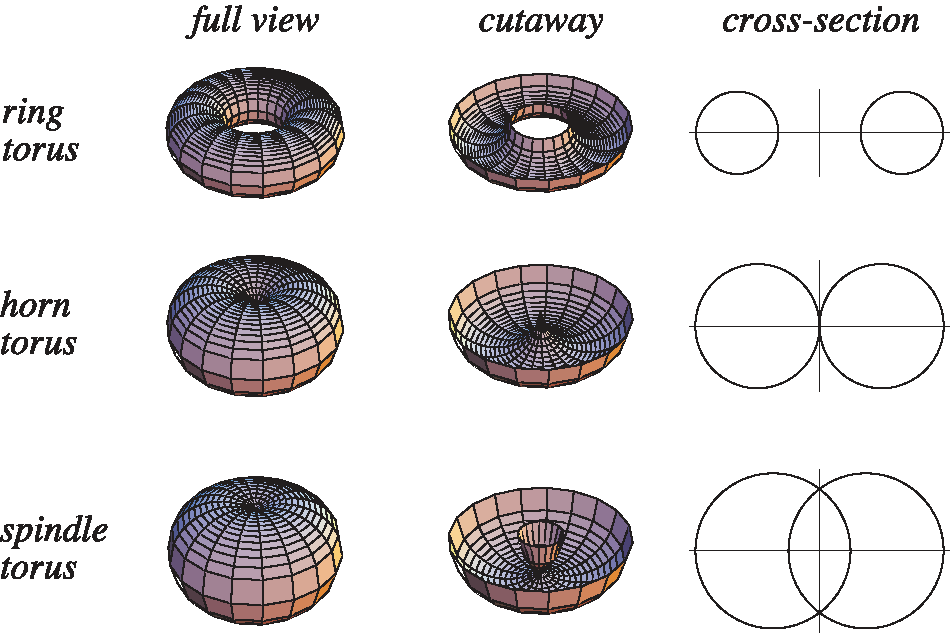
\includegraphics[width=0.7\linewidth]{pic/StandardTori701.pdf}
        \caption{StandardTori701}
        \label{fig:StandardTori701}
    \end{figure}
    If we think of $\mathbf{N} = \mathbf{N}(u, v)$ as a directed line segment, 
    pointing from $\Phi(u, v)$ to $\Phi(u, v) + \mathbf{N}(u, v)$, 
    then $\mathbf{N}$ points outward, 
    that is to say, away from $\Psi(K)$. 
    This is so because $\mathbf{J}_{\Psi} > 0$ when $t = a$.

    For example, take $u = v = \pi/2$, $t = a$. 
    This gives the largest value of $z$ on $\Psi(K)$, 
    and $\mathbf{N} = a(b + a)\mathbf{e}_3$ points ``upward'' for this choice of $(u, v)$.
\end{newexample}

\begin{mydef}
    \label{mydef:10.48}
    \myKeyword{Integrals of 1-forms in $\R^3$}
    Let $\gamma$ be a $\mathscr{C}'$-curve in an open set $E \subset \R^3$, with parameter interval $[0, 1]$, 
    let $\mathbf{F}$ be a vector field in $E$, as in Sec. \ref{mydef:10.42}, 
    and define $\lambda_{\mathbf{F}}$, by \eqref{eq:10.124}. 
    The integral of $\lambda_{\mathbf{F}}$, over $\gamma$ can be rewritten in a certain way which we now describe.

    For any $u \in [0,1]$,
    \begin{equation*}
        \gamma' (u) = 
        \gamma'_1 (u) \mathbf{e}_1 +
        \gamma'_2 (u) \mathbf{e}_2 +
        \gamma'_3 (u) \mathbf{e}_3 
    \end{equation*}
    is called the \myKeyword{tangent vector} to $\gamma$ at $u$. 
    We define $\mathbf{t} = \mathbf{t}(u)$ to be the unit vector in the direction of $\gamma'(u)$. 
    Thus
    \begin{equation*}
        \gamma'(u) = \left| \gamma'(u) \right| \mathbf{t} (u) .
    \end{equation*}
    [If $\gamma'(u) = \mathbf{0}$ for some $u$, 
    put $\mathbf{t}(u) = \mathbf{e}_1$; 
    any other choice would do just as well.]
    By \eqref{eq:10.35},
    \begin{equation}
        \label{eq:10.142}
        \begin{aligned}
            \int_{\gamma} \lambda_{\mathbf{F}}
            &= \sum_{i=1}^{3} \int_{0}^{1} F_i (\gamma(u)) \gamma'_i(u) \d u \\
            &= \int_{0}^{1} \mathbf{F} (\gamma(u)) \cdot \gamma'(u) \d u \\
            &= \int_{0}^{1} \mathbf{F} (\gamma(u)) \cdot \mathbf{t}(u) \left| \gamma'(u) \right| \d u .
        \end{aligned}
    \end{equation}

    Theorem \ref{thm:6.27} makes it reasonable to call $| \gamma'(u) | \d u$ the \myKeywordblue{element of arc length along} $\gamma$. 
    A customary notation for it is $\d s$, and \eqref{eq:10.142} is rewritten in the form
    \begin{equation}
        \label{eq:10.143}
        \int_{\gamma} \lambda_{\mathbf{F}}
        = \int_{\gamma} (\mathbf{F \cdot t}) \d s .
    \end{equation}

    Since $\mathbf{t}$ is a unit tangent vector to $\gamma$, 
    $\mathbf{F \cdot t}$ is called the \myKeywordblue{tangential component} of $\mathbf{F}$ along $\gamma$.

    The right side of \eqref{eq:10.143} should be regarded as just an abbreviation for the last integral in \eqref{eq:10.142}. 
    The point is that $\mathbf{F}$ is defined on the range of $\gamma$, but $\mathbf{t}$ is defined on $[0, 1]$; 
    thus $\mathbf{F \cdot t}$ has to be properly interpreted. 
    Of course, when $\gamma$ is one-to-one, 
    then $\mathbf{t}(u)$ can be replaced by $\mathbf{t}(y(u))$, and this difficulty disappears.
\end{mydef}

\begin{mydef}
    \label{mydef:10.49}
    \myKeyword{Integrals of 2-forms in $\R^3$}
    Let $\Phi$ be a 2-surface in an open set $E \subset \R^3$,
    of class $\mathscr{C}'$, with parameter domain $D \subset \R^2$. 
    Let $\mathbf{F}$ be a vector field in $E$, and define $\omega_{\mathbf{F}}$ by \eqref{eq:10.125}. 
    As in the preceding section, we shall obtain a different representation of the integral of $\omega_{\mathbf{F}}$ over $\Phi$.

    By \eqref{eq:10.35} and \eqref{eq:10.129},
    \begin{align*}
        \int_{\Phi} \omega_{\mathbf{F}} 
        &= \int_{\Phi} \left( 
            F_1 \d y \wedge \d z + 
            F_2 \d z \wedge \d x + 
            F_3 \d x \wedge \d y  
            \right) \\
        &= \int_{D} \left\{ 
            (F_1 \circ \Phi) \frac{\partial (y,z)}{\partial (u,v)} + 
            (F_2 \circ \Phi) \frac{\partial (z,x)}{\partial (u,v)} + 
            (F_3 \circ \Phi) \frac{\partial (x,y)}{\partial (u,v)} 
         \right\} \d u \d v \\
        &= \int_{D} \mathbf{F}(\Phi(u,v))\cdot \mathbf{N}(u,v) \d u \d v .
    \end{align*}
    Now let $\mathbf{n} = \mathbf{n}(u, v)$ be the unit vector in the direction of $\mathbf{N}(u, v)$. 
    [If $\mathbf{N}(u, v) = 0$ for some $(u, v) \in D$, 
    take $\mathbf{n}(u, v) = \mathbf{e}_1$.] 
    Then $\mathbf{N = |N |n}$, and therefore the last integral becomes
    \begin{equation*}
        \int_{D} \mathbf{F}(\Phi(u,v)\cdot \mathbf{n}(u,v))
        \left| \mathbf{N}(u,v) \right| \d u \d v .
    \end{equation*}
    By \eqref{eq:10.131}, we can finally write this in the form
    \begin{equation}
        \label{eq:10.144}
        \int_{\Phi} \omega_{\mathbf{F}} = 
        \int_{\Phi} (\mathbf{F \cdot n}) \d A .
    \end{equation}
    With regard to the meaning of $\mathbf{F \cdot n}$, 
    the remark made at the end of Sec. \ref{mydef:10.48} applies here as well.
\end{mydef}

We can now state the original form of Stokes' theorem.

\begin{thm}
    \label{thm:10.50}
    \myKeyword{Stokes' formula}
    If $\mathbf{F}$ is a vector field of class $\mathscr{C}'$ in an open set $E \subset \R^3$, 
    and if $\Phi$ is a 2-surface of class $\mathscr{C}''$ in $E$, then
    \begin{equation}
        \label{eq:10.145}
        \int_{\Phi} \left( \nabla \times \mathbf{F} \right) \cdot \mathbf{n} \d A = 
        \int_{\partial \Phi} \left( \mathbf{F \cdot t} \right)  \d s
    \end{equation}
\end{thm}

\begin{proof}
    Put $\mathbf{H} = \nabla \times \mathbf{F}$.
    Then, as in the proof of Theorem \ref{thm:10.43},
    we have 
    \begin{equation}
        \label{eq:10.146}
        \omega_{\mathbf{H}} = \d \lambda_{\mathbf{F}} . 
    \end{equation}
    Hence 
    \begin{align*}
        \int_{\Phi} (\nabla \times \mathbf{F}) \cdot \mathbf{n} \d A 
        &= \int_{\Phi} (\mathbf{H \cdot n}) \d A 
        = \int_{\Phi} \omega_{\mathbf{H}} \\
        &= \int_{\Phi} \d \lambda_{\mathbf{F}} 
        = \int_{\partial \Phi} \lambda_{\mathbf{F}} 
        = \int_{\partial \Phi} (\mathbf{F \cdot t}) \d s .
    \end{align*}
    Here we used the definition of $\mathbf{H}$, 
    then \eqref{eq:10.144} with $\mathbf{H}$ in place of $\mathbf{F}$, 
    then \eqref{eq:10.146}, then-the main step-Theorem \ref{thm:10.33}, 
    and finally \eqref{eq:10.143}, extended in the obvious way from curves to 1-chains.
\end{proof}

\begin{thm}
    \label{thm:10.51}
    \myKeyword{The divergence theorem}
    If $\mathbf{F}$ is a vector field of class $\mathscr{C}'$ in an open set $E \subset \R^3$, 
    and if $\Omega$ is a closed subset of $E$ with positively oriented boundary $\partial \Omega$ (as described in Sec. \ref{mydef:10.31}) then
    \begin{equation}
        \label{eq:10.147}
        \int_{\Omega} \left( \nabla \cdot \mathbf{F} \right) \d V 
        \int_{\partial \Omega} \left( \mathbf{F} \cdot \mathbf{n} \right) \d A . 
    \end{equation}
\end{thm}

\begin{proof}
    By \eqref{eq:10.125}
    \begin{equation*}
        \d \omega_{\mathbf{F}} = 
        (\nabla \cdot \mathbf{F}) \d x \wedge \d y \wedge \d z = 
        (\nabla \cdot \mathbf{F}) \d V .
    \end{equation*}
    Hence 
    \begin{equation*}
        \int_{\Omega} (\nabla \cdot \mathbf{F}) \d V
        = \int_{\Omega} \d \omega_{\mathbf{F}} 
        = \int_{\partial \Omega} \omega_{\mathbf{F}} 
        = \int_{\partial \Omega} (\mathbf{F \cdot n}) \d A ,
    \end{equation*}
    by Theorem \ref{thm:10.33}, 
    applied to the 2-form $\omega_{\mathbf{F}}$, and \eqref{eq:10.144}.
\end{proof}

% chap10exercise

\section{Exercises}


\begin{myexercise}
    \label{ex:10.1}
    Let $H$ be a compact convex set in $\R^k$, with nonempty interior.
    Let $f \in \mathscr{C}(H)$, put $f(\mathbf{x}) = 0$ in the complement of $H$,
    and define $\int_H f$ as in Definition \ref{mydef:10.3}.

    Prove that $\int_H f$ is independent of the order in which the $k$ integrations are carried out.

    \emph{Hint:} Approximate $f$ by functions that are continuous on $\R^k$ and whose supports are in $H$, as was done in Example \ref{newexample:10.47}.
\end{myexercise}


\begin{myexercise}
    \label{ex:10.2}
    For $i = 1, 2, 3, ...$ , let $\phi_i \in \mathscr{C}(\R^1)$ have support in $(2^{-i} , 2^{1-i})$, such that $\int \phi_i = 1$.
    Put
    \begin{equation*}
        f(x,y) = \sum_{i=1}^{\infty}
        \left[
            \phi_{i}(x) -
            \phi_{i+1}(x)
            \right] \phi_i (y)
    \end{equation*}
    Then $f$ has compact support in $\R^2$,
    $f$ is continuous except at $(0,0)$,
    and
    \begin{equation*}
        \int \d y \int f(x,y) \d x = 0
        \quad \text{ but } \quad
        \int \d x \int f(x,y) \d y = 1.
    \end{equation*}
    Observe that $f$ is unbounded in every neighborhood of $(0, 0)$.
\end{myexercise}


\begin{myexercise}
    \label{ex:10.3}
    \begin{asparaenum}[(a)]
        \item If $F$ is as in Theorem \ref{thm:10.7}, put
        $\mathbf{A} = \mathbf{F}'(0)$,
        $\mathbf{F_{1}(x)} = \mathbf{A^{-1}F(x)}$.
        Then $\mathbf{F'_1(0)}=I$.
        Show that
        \begin{equation*}
            \mathbf{F_1(x) = G_n \circ G_{n-1} \circ \cdots \circ G_1(x)}
        \end{equation*}
        in some neighborhood of $\mathbf{0}$,
        for certain primitive mappings $\mathbf{G_n \circ \cdots \circ G_1(x)}$.
        This gives another version of Theorem \ref{thm:10.7}:
        \begin{equation*}
            \mathbf{F(x) = F'(0) G_n \circ G_{n-1} \circ \cdots \circ G_1(x)}.
        \end{equation*}
        \item Prove that the mapping $(x, y) > (y, x)$ of $\R^2$ onto $\R^2$ is not the composition of any two primitive mappings, in any neighborhood of the origin.
        (This shows that the flips $B_1$ cannot be omitted from the statement of Theorem \ref{thm:10.7}.)
    \end{asparaenum}
\end{myexercise}

\begin{myexercise}
    \label{ex:10.4}
    For $(x,y) \in \R^2$, define
    \begin{equation*}
        \mathbf{F}(x,y) = (e^x \cos y - 1, e^x \sin y).
    \end{equation*}
    Prove that $\mathbf{F = G_2 \circ G_1}$, where
    \begin{align*}
        \mathbf{G}_1 (x,y) & = (e^x \cos y - 1, y) \\
        \mathbf{G}_2 (u,v) & = (u, (1 + u) \tan v)
    \end{align*}
    are primitive in some neighborhood of $(0, 0)$.

    Compute the Jacobians of $\mathbf{G_1, G_2, F}$ at $(0, 0)$.
    Define
    \begin{equation*}
        \mathbf{H}_2 (x,y) = (x, e^x \sin y)
    \end{equation*}
    and find
    \begin{equation*}
        \mathbf{H}_1 (u,v) = (h(u,v), v)
    \end{equation*}
    so that $\mathbf{F = H_1 \circ H_2}$ is some neighborhood of $(0,0)$.
\end{myexercise}


\begin{myexercise}
    \label{ex:10.5}
    Formulate and prove an analogue of Theorem \ref{thm:10.8},
    in which $K$ is a compact subset of an arbitrary metric space.
    (Replace the functions $\phi_i$ that occur in the
    proof of Theorem \ref{thm:10.8}
    by functions of the type constructed in Exercise \ref{ex:4.22})
\end{myexercise}


\begin{myexercise}
    \label{ex:10.6}
    Strengthen the conclusion of Theorem \ref{thm:10.8} by showing that the functions $\psi_i$ can be made differentiable, and even infinitely differentiable.
    (Use Exercise \ref{ex:8.1} in the construction of the auxiliary functions $\phi_i$.)
\end{myexercise}


\begin{myexercise}
    \label{ex:10.7}
    \begin{enumerate}[(a)]
        \item Show that the simplex $Q^k$ is the smallest convex subset of $\R^k$ that contains $\mathbf{0},\mathbf{e}_1,\dots,\mathbf{e}_k$.
        \item Show that affine mappings take convex sets to convex sets.
    \end{enumerate}
\end{myexercise}


\begin{myexercise}
    \label{ex:10.8}
    Let $H$ be the parallelogram in $\R^2$ whose vertices are $(1, 1), (3, 2), (4, 5), (2, 4)$.
    Find the affine map $T$ which sends $(0, 0)$ to $(1, 1)$, $(1, 0)$ to $(3, 2)$, $(0, 1)$ to $(2, 4)$.
    Show that $J_T = 5$.
    Use $T$ to convert the integral
    \begin{equation*}
        \alpha = \int_H e^{x-y} \d x \d y
    \end{equation*}
    to an integral over $I^2$ and thus compute $\alpha$.
\end{myexercise}


\begin{myexercise}
    \label{ex:10.9}
    Define $(x, y) = T(r, \theta)$ on the rectangle
    \begin{equation*}
        0 \leq r \leq a,
        \quad
        0 \leq \theta \leq 2\pi
    \end{equation*}
    by the equations
    \begin{equation*}
        x = r \cos \theta , \quad
        y = r \sin \theta .
    \end{equation*}
    Show that $T$ maps this rectangle onto the closed disc $D$ with center at $(0, 0)$ and radius $a$,
    that $T$ is one-to-one in the interior of the rectangle, and that $J_T(r, \theta) = r$.
    If $f \in \mathscr{C}(D)$, prove the formula for integration in polar coordinates:
    \begin{equation*}
        \int_D f(x,y) \d x \d y =
        \int_{0}^{a} \int_{0}^{2\pi} f(T(r,\theta)) r \d r \d \theta .
    \end{equation*}
    \emph{Hint:} Let Do be the interior of $D$, minus the interval from $(0, 0)$ to $(0, a)$.
    As it stands, Theorem \ref{thm:10.9} applies to continuous functions $f$ whose support lies in $D_0$.
    To remove this restriction, proceed as in Example \ref{newexample:10.4}.
\end{myexercise}



\begin{myexercise}
    \label{ex:10.10}
    Let $a \rightarrow \infty$ in \ref{ex:11.9} and prove that
    \begin{equation*}
        \int_{\R^2} f(x,y) \d x \d y =
        \int_{0}^{\infty} \int_{0}^{2\pi} f(T(r,\theta)) r \d r \d \theta ,
    \end{equation*}
    for continuous functions f that decrease sufficiently rapidly as $|x | + | y | \rightarrow \infty$.
    (Find a more precise formulation.)
    Apply this to
    \begin{equation*}
        f(x, y) = \exp (-x^2 - y^2)
    \end{equation*}
    to derive formula \eqref{eq:8.101}.
\end{myexercise}


\begin{myexercise}
    \label{ex:10.11}
    Define $(u,v)=T(s,t)$ on the strip
    \begin{equation*}
        0<s<\infty , \quad
        0<t<1
    \end{equation*}
    by setting $u = s - st$, $v = st$.
    Show that $T$ is a 1-1 mapping of the strip onto the positive quadrant $Q$ in $\R^2$.
    Show that $J_T(s, t) = s$.

    For x > 0, y > 0, integrate
    \begin{equation*}
        u^{x-1} e^{-u} v^{y-1} e^{-v}
    \end{equation*}
    over $Q$, use Theorem \ref{thm:10.9} to convert the integral to one over the strip, and derive formula \eqref{eq:8.96} in this way.
    (For this application, Theorem \ref{thm:10.9} has to be extended so as to cover certain improper integrals.
    Provide this extension.)
\end{myexercise}


\begin{myexercise}
    \label{ex:10.12}
    Let $I^k$ be the set of all $\mathbf{u} = (u_1, ... , u_k) \in \R^k$ with $0 \leq u_i \leq 1$ for all $i$;
    let $Q^k$ be the set of all $\mathbf{x} = (x_1, ... , x_k) \in  \R^k$ with $x_i \geq 0, \sum x_i \leq 1$.
    ($I^k$ is the unit cube;
    $Q^k$ is the standard simplex in $\R^k$.)
    Define $\mathbf{x} = T(\mathbf{u})$ by
    \begin{align*}
        x_1   & = u_1                          \\
        x_2   & = (1-u_1)u_2                   \\
        \dots & \dots
        x_k   & = (1-u_1)\cdots(1-u_{k-1})u_k.
    \end{align*}
    Show that
    \begin{equation*}
        \sum_{i=1}^{k} x_i = 1 - \prod_{i=1}^{k} (1-u_i) .
    \end{equation*}

    Show that $T$ maps $I^k$ onto $Q^k$,
    that $T$ is 1-1 in the interior of $I^k$,
    and that its inverse $S$ is defined in the interior of $Q^k$ by $u_1 = x_1$ and
    \begin{equation*}
        u_i = \frac{x_i}{1-x_1-\cdots-x_{i-1}}
    \end{equation*}
    for $i=2,\dots,k$.
    Show that
    \begin{equation*}
        J_T(\mathbf{u}) =
        (1-u_1)^{k-1}
        (1-u_2)^{k-2}
        \cdots
        (1-u_{k-1}),
    \end{equation*}
    and
    \begin{equation*}
        J_S(\mathbf{x}) =
        \left[
            (1-x_1)
            (1-x_1-x_2)
            \cdots
            (1-x_1-\cdots-x_{k-1})
            \right]^{-1} .
    \end{equation*}
\end{myexercise}


\begin{myexercise}
    \label{ex:10.13}
    Let $r_1,\dots,r_k$ be nonnegative integers, and prove that
    \begin{equation*}
        \int_{Q^k}
        x_1^{r_1}
        \cdots
        x_k^{r_k}
        \d x =
        \frac{r_1!\cdots r_k!}{(k+r_1+\cdots+r_k)!}
    \end{equation*}
    \emph{Hint:} Use Exercise \ref{ex:11.12}, Theorem \ref{thm:10.9} and \ref{thm:8.20}.

    Note that the special case $r_1 = \cdots = r_k = 0$
    shows that the volume of $Q^k$ is $1/k!$.
\end{myexercise}


\begin{myexercise}
    \label{ex:10.14}
    Prove formula \eqref{eq:10.46}.
\end{myexercise}


\begin{myexercise}
    \label{ex:10.15}
    If $\omega$ and $\lambda$ are $k$- and $m$-forms, respectively, prove that
    \begin{equation*}
        \omega \wedge \lambda =
        (-1)^{km} \lambda \wedge \omega .
    \end{equation*}
\end{myexercise}


\begin{myexercise}
    \label{ex:10.16}
    If $k \geq 2$ and $\delta = [\mathbf{p}_0, \mathbf{p}_1, ... , \mathbf{p}_t]$ is an oriented affine $k$-simplex,
    prove that $\partial^2 \sigma = 0$,
    directly from the definition of the boundary operator $\partial$.
    Deduce from this that $\partial^2 \Psi = 0$ for every chain $\Psi$.

    \emph{Hint:} For orientation, do it first for $k= 2, k = 3$.
    In general, if $i <j$, let $\sigma_{ij}$ be the $(k - 2)$-simplex obtained by deleting $\mathbf{p}_i$ and $\mathbf{p}_j$ from $u$.
    Show that each $\sigma_{ij}$ occurs twice in $\partial^2 \sigma$, with opposite sign.
\end{myexercise}


\begin{myexercise}
    \label{ex:10.17}
    Put $J^2 = \tau_1 + \tau_2$, where
    \begin{equation*}
        \tau_1 =  \left[ \mathbf{0,e_1,e_1+e_2} \right],
        \quad
        \tau_2 = -\left[ \mathbf{0,e_2,e_2+e_1} \right].
    \end{equation*}
    Explain why it is reasonable to call $J^2$ the positively oriented unit square in $\R^2$ .
    Show that $\partial J^2$ is the sum of 4 oriented affine 1-simplexes. Find these. What is $\partial (\tau_1 - \tau_2)$?
\end{myexercise}


\begin{myexercise}
    \label{ex:10.18}
    Consider the oriented affine 3-simplex
    \begin{equation*}
        \sigma_1 =  \left[ \mathbf{0,e_1,e_1+e_2,e_1+e_2+e_3} \right]
    \end{equation*}
    in $\R^3$.
    Show that $\sigma_1$
    (regarded as a linear transformation) has determinant 1.
    Thus $\sigma_1$ is positively oriented.

    Let $\sigma_2 , ... , \sigma_6$ be five other oriented 3-simplexes, obtained as follows:
    There are five permutations $(i_1, i_2, i_3)$ of $(1, 2, 3)$, distinct from $(1, 2, 3)$.
    Associate with each $(i_1, i_2, i_3)$ the simplex
    \begin{equation*}
        s(i_1, i_2, i_3) \left[ \mathbf{0,e_{i_1},e_1+e_2} \right]
    \end{equation*}
    where $s$ is the sign that occurs in the definition of the determinant.
    (This is how $\tau_2$ was obtained from $\tau_1$ in Exercise \ref{ex:11.17}.)

    Show that $\sigma_2, \dots , \sigma_6$ are positively oriented.

    Put $J^3 = \sigma_1 + \dots + \sigma_6$.
    Then $J^3$ may be called the positively oriented unit cube in $\R^3$.

    Show that $\partial J^3$ is the sum of 12 oriented affine 2-simplexes.
    (These 12 triangles cover the surface of the unit cube $I^3$,)

    Show that $\mathbf{x} = (\mathbf{x}_1, \mathbf{x}_2, \mathbf{x}_3)$ is in the range of $\sigma_1$ if and only if $0 \leq x_3 \leq x_2 \leq x_1 \leq 1$,

    Show that the ranges of $\sigma_1, ... , \sigma_6$ have disjoint interiors, and that their union covers $I^3$.
    (Compare with Exercise \ref{ex:11.13}; note that $3! = 6$.)
\end{myexercise}


\begin{myexercise}
    \label{ex:10.19}
    Let $J^2$ and $J^3$ be as in Exercise \ref{ex:11.17} and \ref{ex:11.18}.
    Define
    \begin{align*}
        B_{01}(u,v) = (0,u,v), & B_{11}(u,v) = (1,u,v), \\
        B_{02}(u,v) = (u,0,v), & B_{12}(u,v) = (u,1,v), \\
        B_{03}(u,v) = (u,v,0), & B_{13}(u,v) = (u,v,1), \\
    \end{align*}
    These are affine, and map $\R^2$ into $\R^3$.

    Put $\beta_{ri} = B_{ri}(J^2)$, for $r = 0,1$, $i=1,2,3$.
    Each $\beta_{ri}$ is an affine-oriented 2-chain.
    (See Sec. \ref{mydef:10.30}.)
    Verify that
    \begin{equation*}
        \partial J^3 = \sum_{i=1}^{3}(-1)^i (\beta_{0i}-\beta_{1i}),
    \end{equation*}
    in agreement with Exercise \ref{ex:10.18}.
\end{myexercise}



\begin{myexercise}
    \label{ex:10.20}
    State conditions under which the formula
    \begin{equation*}
        \int_{\Phi} f \d \omega =
        \int_{\partial\Phi} f \omega -
        \int_{\Phi} (\d f) \wedge \omega
    \end{equation*}
    is valid, and show that it generalizes the formula for integration by parts.

    \emph{Hint:} $\d(f \omega) = (\d f) \wedge \omega + f d\omega$.
\end{myexercise}


\begin{myexercise}
    \label{ex:10.21}
    As in Example \ref{newexample:10.36}, consider the 1-form
    \begin{equation*}
        \eta = \frac{x \d y - y \d x}{x^2+y^2}
    \end{equation*}
    in $\R^2 - \{\mathbf{0}\}$.
    \begin{asparaenum}[(a)]
        \item Carry out the computation that leads to formula \eqref{eq:10.113}, and prove that $\d \eta = 0$.
        \item Let $\gamma(t) = (r \cos t, r \sin t)$, for some $r > 0$,
        and let $r$ be a $\mathscr{C}''$-curve in $\R^2 - \{\mathbf{0}\}$,
        with parameter interval $[0, 2\pi]$, with $\Gamma(0) = \Gamma(2\pi)$, such that the intervals $[\gamma(t), \Gamma(t)]$ do not contain $\mathbf{0}$ for any $t \in $$[0, 2\pi]$. Prove that
            \begin{equation*}
                \int_{\Gamma} \eta = 2 \pi .
            \end{equation*}

            \emph{Hint:} For $0 \leq t \leq 2\pi$, $0 \leq u \leq 1$, define
            \begin{equation*}
                \Phi(t,u)=(1-u)\Gamma(t)+u\gamma(t).
            \end{equation*}
            Then $\Phi$ is a 2-surface in $\R^2 - \{\mathbf{0}\}$ whose parameter domain is the indicated rectangle.
            Because of cancellations (as in Example \ref{newexample:10.32}),
            \begin{equation*}
                \partial \Phi = \Gamma - \gamma .
            \end{equation*}
            Use Stokes' theorem to deduce that
            \begin{equation*}
                \int_{\Gamma} \eta =
                \int_{\gamma} \eta
            \end{equation*}
            because $\d \eta = 0$.
            \item Take $\Gamma(t)=(a \cos t, b \sin t)$ where $a>0,b>0$ are fixed. Use part (b) to show that
            \begin{equation*}
                \int_{0}^{2\pi} \frac{ab}{a^2\cos^2 t + b^2 \sin^2 t} \d t = 2 \pi .
            \end{equation*}
            \item Show that
            \begin{equation*}
                \eta = \d \left( \arctan\frac{y}{x} \right)
            \end{equation*}
            in any convex open set in which $x \neq 0$, and that
            \begin{equation*}
                \eta = \d \left( -\arctan\frac{x}{y} \right)
            \end{equation*}
            in any convex open set in which $y \neq 0$.
            \item Show that (b) can be derived from (d).
            \item If $\Gamma$ is any closed $\mathscr{C}'$-curve in $\R^2 - \{\mathbf{0}\}$, prove that
        \begin{equation*}
            \frac{1}{2\pi} \int_{\Gamma} \eta = \Ind (\Gamma).
        \end{equation*}
        (See Exercise \ref{ex:8.23} for the definition of the index of a curve.)
    \end{asparaenum}
\end{myexercise}


\begin{myexercise}
    \label{ex:10.22}
    As in Example \ref{newexample:10.37}, define $\zeta$ in $\R^3 - \{\mathbf{0}\}$ by
    \begin{equation*}
        \zeta =
        \frac{
            x \d y \wedge \d z +
            y \d z \wedge \d x +
            z \d x \wedge \d y
        }{r^3}
    \end{equation*}
    where $r = \left( x^2+y^2+z^2 \right)^{1/2}$,
    let $D$ be the rectangle given by
    $0 \leq u \leq \pi$,
    $0 \leq v \leq \pi$,
    and let $\sum$ be the 2-surface in $\R^3$,
    with parameter domain in $D$, given by
    \begin{equation*}
        x = \sin u \cos v, \quad
        y = \sin u \sin v, \quad
        z = \cos u .
    \end{equation*}
    \begin{asparaenum}[(a)]
        \item Prove that $\d \zeta = 0$ in $\R^3 - \{\mathbf{0}\}$.
        \item Let $S$ denote the restriction of $\sum$ to a parameter domain $E \subset D$.
        Prove that
        \begin{equation*}
            \int_S \zeta = \int_E \sin u \d u \d v = A(S),
        \end{equation*}
        where $A$ denotes area, as in Sec. \ref{thm:10.43}.
        Note that this contains \eqref{eq:10.115} as a special case.
        \item Suppose $g, h_1, h_2, h_3$, are $\mathscr{C}''$-functions on $[0, 1], g > 0$.
        Let $(x, y, z) = \Phi(s, t)$
        define a 2-surface $\Phi$, with parameter domain $I^2$, by
        \begin{equation*}
            x = g(t)h_1(s) , \quad
            y = g(t)h_2(s) , \quad
            z = g(t)h_3(s) .
        \end{equation*}
        Prove that
        \begin{equation*}
            \int_{\Phi} \zeta = 0 ,
        \end{equation*}
        directly from \eqref{eq:10.35}.

        Note the shape of the range of $\Phi$:
        For fixed $s$, $\Phi(s, t)$ runs over an interval on a line through 0.
        The range of $\Phi$ thus lies in a ``cone'' with vertex at the origin.
        \item Let $E$ be a closed rectangle in $D$, with edges parallel to those of $D$.
        Suppose $f \in \mathscr{C}''(D), f> 0$.
        Let $\Omega$ be the 2-surface with parameter domain $E$, defined by
        \begin{equation*}
            \Omega(u,v) = f(u,v)\sum(u,v).
        \end{equation*}
        Define $S$ as in (b) and prove that
        \begin{equation*}
            \int_{\Phi} \zeta =  \int_{S} \zeta = A(S).
        \end{equation*}
        (Since $S$ is the ``radial projection'' of $n$ into the unit sphere, this result makes it reasonable to call $\int_n \zeta$ the ``solid angle'' subtended by the range of $\Omega$ at the origin.)

        \emph{Hint:} Consider the 3-surface $\Psi$ given by
        \begin{equation*}
            \Psi(t,u,v) = \left[ 1-t+t f(u,v) \right] \sum (u,v) ,
        \end{equation*}
        where $(u, v) \in E$, $0 \leq t \leq 1$.
        For fixed $v$, the mapping $(t, u) \rightarrow \Psi(t, u, v)$ is a 2-surface $\Psi$ to which (c) can be applied to show that $\int_{\Phi} \zeta = 0$.
        The same thing holds when $u$ is fixed.
        By (a) and Stokes' theorem,
        \begin{equation*}
            \int_{\partial \Psi} \zeta =
            \int_{\Psi} \d \zeta = 0.
        \end{equation*}
        \item Put $\lambda = -(z/r)\eta$, where
        \begin{equation*}
            \eta = \frac{x \d y - y \d x}{x^2+y^2} ,
        \end{equation*}
        as in Exercise \ref{ex:10.21}.
        Then $\lambda$ is a 1-form in the open set $V \subset \R^3$ in which $x^2 + y^2 > 0$.
        Show that $\zeta$ is \myKeywordblue{exact in} $V$ by showing that
        \begin{equation*}
            \zeta = \d \lambda .
        \end{equation*}
        \item Derive (d) from (e), without using (c).
        \emph{Hint:} To begin with, assume $0 < u < \pi$ on $E$.
        By (e),
        \begin{equation*}
            \int_{\Omega} \zeta = \int_{\partial \Omega} \lambda
            \quad \text{ and } \quad
            \int_{S} \zeta = \int_{\partial S} \lambda .
        \end{equation*}
        Show that the two integrals of $\lambda$ are equal, by using part (d) of Exercise \ref{ex:10.21},
        and by noting that $z/r$ is the same at $\sum(u, v)$ as at $\Omega(u, v)$.
        \item Is $\zeta$ exact in the complement of every line through the origin?
    \end{asparaenum}
\end{myexercise}


\begin{myexercise}
    \label{ex:10.23}
    Fix $n$.
    Define $r_k = (x_1^2 + \cdots + x_k^2)$ for $1 \leq k \leq n$, let $E_k$ be the set of all $\mathbf{x} \in \R^n$ at which $r_k > 0$, and let $\omega_k$ be the $(k - 1)$-form defined in $E_k$ by
    \begin{equation*}
        \omega_k = (r_k)^{-k} \sum_{i=1}^{k} (-1)^{i-1} x_i
        \d x_1 \wedge \cdots \wedge
        \d x_{i-1} \wedge
        \d x_{i+1} \wedge \cdots \wedge
        \d x_k .
    \end{equation*}
    Note that $\omega_2 = \eta$, $\omega_3 = \zeta$, in the terminology of Exercises \ref{ex:10.21} and \ref{ex:10.22}.
    Note also that
    \begin{equation*}
        E_1 \subset
        E_2 \subset
        \cdots \subset
        E_n = \R^n - \{\mathbf{0}\} .
    \end{equation*}
    \begin{asparaenum}[(a)]
        \item Prove that $\d \omega_k = 0$ in $E_k$.
        \item For $k=2,\dots,n$, prove that $\omega_k$ is exact in $E_{k-1}$, by showing that
        \begin{equation*}
            \omega_k = \d (f_k \omega_{k-1})
            = (\d f_k) \wedge \omega_{k-1} ,
        \end{equation*}
        where $f_k(\mathbf{x})=(-1)^k g_k(x_k/r_k)$ and
        \begin{equation*}
            g_k(t)=\int_{-1}^{t}(1-s^2)^{(k-3)/2} \d s
            \quad (-1<t<1).
        \end{equation*}
        \emph{Hint:} $f_k$ satisfies the differential equations
        \begin{equation*}
            \mathbf{x} \cdot (\nabla f_k)(\mathbf{x}) = 0
        \end{equation*}
        and
        \begin{equation*}
            (D_k f_k)(\mathbf{x}) = \frac{(-1)^k(r_{k-1})^{k-1}}{(r_k)^k}.
        \end{equation*}
        \item Is $\omega_n$ exact in $E_n$?
        \item Note that (b) is a generalization of part (e) of Exercise \ref{ex:10.22}.
        Try to extend some of the other assertions of Exercises \ref{ex:10.21} and \ref{ex:10.22} to $\omega_n$, for arbitrary $n$.
    \end{asparaenum}
\end{myexercise}


\begin{myexercise}
    \label{ex:10.24}
    Let $\omega = \sum a_i(\mathbf{x}) \d x_i$ be a 1-form of class $\mathscr{C}''$ in a convex open set $E \subset \R^n$.
    Assume $\d \omega = 0$ and prove that $\omega$ is exact in $E$, by completing the following outline:

    Fix $\mathbf{p} \in E$.
    Define
    \begin{equation*}
        f(\mathbf{x}) = \int_{[\mathbf{p,x}]} \omega
        \quad
        (\mathbf{x} \in E).
    \end{equation*}
    Apply Stokes' theorem to affine-oriented 2-simplexes $[\mathbf{p, x, y}]$ in $E$.
    Deduce that
    \begin{equation*}
        f(\mathbf{y}) -
        f(\mathbf{x}) =
        \sum_{i=1}^{n} (y_i-x_i)
        \int_{0}^{1} a_i ((1-t)\mathbf{x}+t\mathbf{y}) \d \mathbf{t}
    \end{equation*}
    for
    $\mathbf{x} \in E$ ,
    $\mathbf{y} \in E$ .
    Hence $(D_i f)(\mathbf{x}) = a_i(\mathbf{x})$.
\end{myexercise}


\begin{myexercise}
    \label{ex:10.25}
    Assume that $\omega$ is a 1-form in an open set $E \subset \R^n$ such that
    \begin{equation*}
        \int_{\gamma} \omega = 0
    \end{equation*}
    for every closed curve $\gamma$ in $E$, of class $\mathscr{C}'$.
    Prove that $\omega$ is exact in $E$, by imitating part of the argument sketched in Exercise \ref{ex:10.24}.
\end{myexercise}


\begin{myexercise}
    \label{ex:10.26}
    Assume $\omega$ is a 1-form in $\R^3-\{\mathbf{0}\}$, of class $\mathscr{C}'$ and $\d \omega =0$.
    Prove that w is exact in $\R^3-\{\mathbf{0}\}$.

    \emph{Hint:} Every closed continuously differentiable curve in $\R^3-\{\mathbf{0}\}$ is the boundary of a 2-surface in $\R^3-\{\mathbf{0}\}$.
    Apply Stokes' theorem and Exercise \ref{ex:10.25}.
\end{myexercise}


\begin{myexercise}
    \label{ex:10.27}
    Let $E$ be an open 3-cell in $\R^3$, with edges parallel to the coordinate axes.
    Suppose $(a, b, c) \in E$, $f_i \in \mathscr{C}'(E)$ for $i = 1, 2, 3$,
    \begin{equation*}
        \omega =
        f_1 \d y \wedge \d z +
        f_2 \d z \wedge \d x +
        f_3 \d x \wedge \d y ,
    \end{equation*}
    and assume that $\d \omega = 0$ in $E$.
    Define
    \begin{equation*}
        \lambda = g_1 \d x + g_2 \d y
    \end{equation*}
    where
    \begin{align*}
        g_1(x,y,z) & = \int_{c}^{z} f_2(x,y,s) \d s - \int_{b}^{y} f_3(x,t,c) \d t \\
        g_2(x,y,z) & = -\int_{c}^{z} f_1(x,y,s) \d s ,
    \end{align*}
    for $(x, y, z) \in E$.
    Prove that $\d \lambda = \omega$ in $E$.

    Evaluate these integrals when $\omega = \zeta$ and thus find the form $\lambda$ that occurs in part (e) of Exercise \ref{ex:10.22}.
\end{myexercise}


\begin{myexercise}
    \label{ex:10.28}
    Fix $b > a > 0$, define
    \begin{equation*}
        \Phi(r, \theta) = (r \cos \theta, r \sin \theta)
    \end{equation*}
    for $a \leq r \leq b, 0 \leq \theta \leq 2\pi$.
    (The range of $\Phi$ is an annulus in $\R^2$.)
    Put $\omega = x^3 \d y$,
    and compute both
    \begin{equation*}
        \int_{\Phi} \d \omega
        \quad \text{and} \quad
        \int_{\partial \Phi} \omega
    \end{equation*}
    to verify that they are equal.
\end{myexercise}


\begin{myexercise}
    \label{ex:10.29}
    Prove the existence of a function $\alpha$ with the properties needed in the proof of Theorem \ref{thm:10.38},
    and prove that the resulting function $F$ is of class $\mathscr{C}'$.
    (Both assertions become trivial if $E$ is an open cell or an open ball,
    since $\alpha$ can then be taken to be a constant.
    Refer to Theorem \ref{thm:9.42}.)
\end{myexercise}



\begin{myexercise}
    \label{ex:10.30}
    If $N$ is the vector given by \eqref{eq:10.135},
    prove that
    \begin{equation*}
        \det
        \begin{bmatrix}
            \alpha_1 & \beta_1 & \alpha_2 \beta_3 - \alpha_3 \beta_2 \\
            \alpha_2 & \beta_2 & \alpha_3 \beta_1 - \alpha_1 \beta_3 \\
            \alpha_3 & \beta_3 & \alpha_1 \beta_2 - \alpha_2 \beta_1 \\
        \end{bmatrix} =
        \left| \mathbf{N} \right|^2 .
    \end{equation*}
    Also, verify Eq. \eqref{eq:10.137}.
\end{myexercise}


\begin{myexercise}
    \label{ex:10.31}
    Let $E \subset \R^3$ be open,
    suppose $g \in  \mathscr{C}''(E)$, $h \in \mathscr{C}''(E)$, and consider the vector field
    \begin{equation*}
        \mathbf{F} = g \nabla h .
    \end{equation*}
    \begin{asparaenum}[(a)]
        \item Prove that
        \begin{equation*}
            \nabla \cdot F = g \nabla^2 h + (\nabla g) \cdot (\nabla h)
        \end{equation*}
        where $\nabla^2 h = \nabla \cdot (\nabla h) = \sum \partial^2 h/ \partial x_i^2$ is the so-called ``\myKeywordblue{Laplacian}'' of $h$.
        \item If $\Omega$ is a closed subset of $E$ with positively oriented boundary $\partial\Omega$ (as in Theorem \ref{thm:10.51}), prove that
        \begin{equation*}
            \int_{\Omega} \left[
                g \nabla^2 h +
                (\nabla g) \cdot (\nabla h)
                \right] \d V =
            \int_{\Omega} \mathbf{g} \frac{\partial h}{\partial n} \d A
        \end{equation*}
        where (as is customary) we have written $\partial h/\partial n$ in place of $(\nabla h) \delta \mathbf{n}$.
        (Thus $\partial h/\partial n$ is the directional derivative of $h$ in the direction of the outward normal to $\partial n$,
        the so-called \myKeywordblue{normal derivative} of $h$.)
        Interchange $g$ and $h$, subtract the resulting formula from the first one, to obtain
        \begin{equation*}
            \int_{\Omega} \left(
            g \nabla^2 h -
            h \nabla^2 g
            \right) \d V =
            \int_{\partial \Omega} \left(
            g \frac{\partial h}{\partial n} -
            h \frac{\partial g}{\partial n}
            \right) \d A .
        \end{equation*}
        These two formulas are usually called \myKeywordblue{Green's identities}.
        \item Assume that $h$ is \myKeywordblue{harmonic} in $E$; this means that $\nabla^2 h = 0$.
        Take $g = 1$ and conclude that
        \begin{equation*}
            \int_{\partial\Omega} \frac{\partial h}{\partial n} \d A = 0.
        \end{equation*}
        Take $g = h$, and conclude that $h = 0$ in $\Omega$ if $h = 0$ on $\partial\Omega$.
        \item Show that Green's identities are also valid in $\R^2$.
    \end{asparaenum}
\end{myexercise}


\begin{myexercise}
    \label{ex:10.32}
    Fix $\delta$, $0 < \delta < 1$.
    Let $D$ be the set of all $(0, t) \in \R^2$ such that $0 \leq \delta \leq \pi$, $-\delta \leq t \leq \delta$.
    Let $\Phi$ be the 2-surface in $\R^3$, with parameter domain $D$, given by
    \begin{align*}
        x & = (1-t \sin \theta) \cos 2 \theta \\
        y & = (1-t \sin \theta) \sin 2 \theta \\
        z & = t \cos \theta
    \end{align*}
    where $(x, y, z) = \Phi(0, t)$.
    Note that $\Phi(\pi, t) = \Phi(0, - t),$
    and that $\Phi$ is one-to-one on the rest of $D$.

    The range $M = \Phi(D)$ of $\Phi$ is known as a \myKeywordblue{M{\"o}bius band}.
    It is the simplest example of a nonorientable surface.

    Prove the various assertions made in the following description:
    Put
    $\mathbf{p}_1 = (0   , -\delta)$,
    $\mathbf{p}_2 = (\pi , -\delta)$,
    $\mathbf{p}_3 = (\pi ,  \delta)$,
    $\mathbf{p}_4 = (0   ,  \delta)$,
    $\mathbf{p}_5 = \mathbf{p}_1$,
    Put $\gamma_i =[\mathbf{p}_{i}, \mathbf{p}_{i+1}]$,
    $i = 1, ... , 4$, and put $\Gamma_i = \Phi \circ \gamma_i$.
    Then
    \begin{equation*}
        \partial \Phi =
        \Gamma_1 +
        \Gamma_2 +
        \Gamma_3 +
        \Gamma_4 .
    \end{equation*}
    Put $\mathbf{a} = (1, 0, -\delta)$, $\mathbf{b} = (1, 0, \delta)$.
    Then
    \begin{equation*}
        \Phi(\mathbf{p}_1) = \Phi(\mathbf{p}_3) = \mathbf{a}, \quad
        \Phi(\mathbf{p}_2) = \Phi(\mathbf{p}_4) = \mathbf{b},
    \end{equation*}
    and $\partial\Phi$ can be described as follows.

    $\Gamma_1$ spirals up from $\mathbf{a}$ to $\mathbf{b}$;
    its projection into the $(x, y)$-plane has winding number $+1$ around the origin. (See Exercise \ref{ex:8.23}.)

    $\Gamma_2 = [b, a]$.

    $\Gamma_3$ spirals up from $\mathbf{a}$ to $\mathbf{b}$;
    its projection into the $(x, y)$ plane has winding number $-1$ around the origin.

    $\Gamma_4 = [b, a]$.

    Thus $\partial\Phi =  \Gamma_1 +  \Gamma_3 + 2 \Gamma_2$.

    If we go from $\mathbf{a}$ to $\mathbf{b}$ along $\Gamma_1$ and continue along the ``edge'' of $M$ until we return to $\mathbf{a}$,
    the curve traced out is
    \begin{equation*}
        \Gamma =
        \Gamma_1 -
        \Gamma_3 ,
    \end{equation*}
    which may also be represented on the parameter interval $[0, 2\pi]$ by the equations
    \begin{align*}
        x & = (1 + \delta \sin \theta) \cos 2 \theta \\
        y & = (1 + \delta \sin \theta) \sin 2 \theta \\
        z & = -\delta \cos \theta .
    \end{align*}
    It should be emphasized that $\Gamma \neq \partial\Phi$:
    Let $\eta$ be the 1-form discussed in Exercises \ref{ex:10.21} and \ref{ex:10.22}.
    Since $d\eta = 0$, Stokes' theorem shows that
    \begin{equation*}
        \int_{\partial\Omega} \eta = 0,
    \end{equation*}
    But although $\Gamma$ is the ``geometric'' boundary of $M$, we have
    \begin{equation*}
        \int_{\Gamma} \eta = 4 \pi .
    \end{equation*}
    In order to avoid this possible source of confusion, Stokes' formula
    (Theorem \ref{thm:10.50}) is frequently stated only for orientable surfaces $\Phi$.
\end{myexercise}




% chap11
\chapter{The lebesgue theory}
\label{chap:11}

It is the purpose of this chapter to present the fundamental concepts of the
Lebesgue theory of measure and integration and to prove some of the crucial
theorems in a rather general setting, without obscuring the main lines of the
development by a mass of comparatively trivial detail. Therefore proofs are
only sketched in some cases, and some of the easier propositions are stated
without proof. However, the reader who has become familiar with the techniques
used in the preceding chapters will certainly find no difficulty in
supplying the missing steps.

The theory of the Lebesgue integral can be developed in several distinct
ways. Only one of these methods will be discussed here. For alternative
procedures we refer to the more specialized treatises on integration listed in
the Bibliography.

% chap11sec01

\section{Set functions}

If $A$ and $B$ are any two sets,
we write $A - B$ for the set of all elements $x$ such that
$x \in A, x \not\in B$.
The notation $A - B$ does not imply that $B \subset A$.
We denote
the empty set by 0,
and say that $A$ and $B$ are disjoint if $A \cap B = 0$.


\begin{mydef}
    A family $\mathscr{R}$ of sets is called a ring if A e $\mathscr{R}$ and Be $\mathscr{R}$ implies
    \begin{equation}
        \label{eq:11.1}
        A \cup B \in \mathscr{R}, \quad
        A - B \in \mathscr{R}.
    \end{equation}
    Since $A n B = A - (A - B)$, we also have $A \cap B \in \mathscr{R}$ if $\mathscr{R}$ is a ring.

    A ring $\mathscr{R}$ is called a $\sigma$-\emph{ring} if
    \begin{equation}
        \label{eq:11.2}
        \bigcup_{n=1}^{\infty} A_n \in \mathscr{R}
    \end{equation}
    whenever $A_n \in \mathscr{R} (n = 1,2,3,\dots)$.
    Since
    \begin{equation*}
        \bigcap_{n=1}^{\infty} A_n
        = A_1 - \bigcup_{n=1}^{\infty} (A_1 - A_n),
    \end{equation*}
    we also have
    \begin{equation*}
        \bigcap_{n=1}^{\infty} A_n \in \mathscr{R}
    \end{equation*}
    if $\mathscr{R}$ is a $\sigma$-ring.
\end{mydef}

\begin{mydef}
    \label{mydef:11.2}
    We say that $\phi$ is a set function defined on $\mathscr{R}$ if $\phi$ assigns to every $A \in \mathscr{R}$ a number $@f(A)$ of the extended real number system.
    $\phi$ is \emph{additive} if $A \cap B = 0$ implies
    \begin{equation}
        \label{eq:11.3}
        \phi \left( A \cup B \right) =
        \phi (A) + \phi (B),
    \end{equation}
    and $\phi$ is \emph{countably additive} if $A_i \cap A_j = 0 (i \neq j)$ implies
    \begin{equation}
        \label{eq:11.4}
        \phi\left( \bigcup_{n=1}^{\infty} A_n \right) =
        \sum_{n=1}^{\infty} \phi\left( A_n \right) .
    \end{equation}
    We shall always assume that the range of $\phi$ does not contain both $+ \infty$ and $- \infty$;
    for if it did, the right side of (\ref{eq:11.3}) could become meaningless.
    Also, we exclude set functions whose only value is $+ \infty$ or $- \infty$.

    It is interesting to note that the left side of (\ref{eq:11.4}) is independent of the order in which the $A_n$'s are arranged.
    Hence the rearrangement theorem shows that the right side of (\ref{eq:11.4}) converges absolutely if it converges at all;
    if it does not converge, the partial sums tend to $+ \infty$, or to $- \infty$.

    If $\phi$ is additive, the following properties are easily verified:
    \begin{align}
        \phi(0) & = 0 \label{eq:11.5}                              \\
        \phi \left( A_1 \cup \cdots \cup A_n \right)
                & = \phi(A_1) + \cdots + \phi(A_n) \label{eq:11.6}
    \end{align}
    if $A_i \cap A_j = 0$ whenever $i \neq j$.
    \begin{equation}
        \label{eq:11.7}
        \phi \left( A_1 \cup A_2 \right) +
        \phi \left( A_1 \cap A_2 \right) =
        \phi (A_1) + \phi (A_2).
    \end{equation}

    If $\phi(A) \geq 0$ for all $A$, and $A_1 \subset A_2$, then
    \begin{equation}
        \label{eq:11.8}
        \phi(A_1) \leq \phi(A_2) .
    \end{equation}

    Because of (\ref{eq:11.8}), nonnegative additive set functions are often called monotonic.
    \begin{equation}
        \label{eq:11.9}
        \phi\left( A - B \right) =
        \phi\left( A \right) -
        \phi\left( B \right)
    \end{equation}
    if $B \subset A$, and $\left| \left( \phi B \right) \right| < +\infty $.
\end{mydef}

\begin{thm}
    \label{thm:11.3}
    Suppose $\phi$ is countably additive on a ring $\mathscr{R}$.
    Suppose $A_n \in \mathscr{R} (n = 1,2,3,\dots)$,
    $A_1 \subset A_2 \subset A_3 \subset \cdots$, $A \in \mathscr{R}$, and
    \begin{equation*}
        A = \bigcup_{n=1}^{\infty} A_n .
    \end{equation*}
    Then, as $n \rightarrow \infty$,
    \begin{equation*}
        \phi(A_n) \rightarrow \phi(A) .
    \end{equation*}
\end{thm}


% chap11sec02

\section{Constriction of the lebesgue measure}

\begin{mydef}
    \label{mydef:11.4}
    Let $\R^p$ denote $p$-dimensional euclidean space.
    By an \emph{interval} in $\R^p$ we mean the set of points $\mathbf{x} = (x_1 , ... , x_p)$ such that
    \begin{equation}
        \label{eq:11.10}
        a_i \leq x_i \leq b_i
        \quad
        (i = 1,\dots,p),
    \end{equation}
    or the set of points which is characterized by (\ref{eq:11.10}) with any or all of the $\leq$ signs replaced by $<$.
    The possibility that $a_i = b_i$ for any value of $i$ is not ruled out;
    in particular, the empty set is included among the intervals.

    If $A$ is the union of a finite number of intervals,
    $A$ is said to be an \emph{elementary set}.

    If $I$ is an interval, we define
    \begin{equation*}
        m(I) = \prod_{i=1}^{p} (b_i - a_i) ,
    \end{equation*}
    no matter whether equality is included or excluded in any of the inequalities (\ref{eq:11.10}).

    If $A = I_1 \cup \cdots \cup I_n$, and if these intervals are pairwise disjoint, we set
    \begin{equation}
        \label{eq:11.11}
        m(A) =
        m(I_1) + \cdots +
        m(I_n) .
    \end{equation}

    We let $\mathscr{E}$ denote the family of all elementary subsets of $\R^p$.

    At this point, the following properties should be verified:
    \begin{enumerate}[(a)]
        \item $\mathscr{E}$ is a ring, but not a $\sigma$-ring.
        \item If $A \in \mathscr{E}$, then $A$ is the union of a finite number of \emph{disjoint} intervals.
        \item If $A \in \mathscr{E}$, $m(A)$ is well defined by (\ref{eq:11.11}); that is. if two different decompositions of $A$ into disjoint intervals are used, each gives rise to the same value of $m(A)$.
        \item $m$ is additive on $\mathscr{E}$
    \end{enumerate}

    Note that if $p = 1,2,3$, then $m$ is length, area, and volume, respectively.
\end{mydef}

\mybox{原书这里的列表项使用公式编号记录...}

\begin{mydef}
    \label{mydef:11.5}
    A nonnegative additive set function $\phi$ defined on $\mathscr{E}$ is said to be regular if the following is true:
    To every $A \in \mathscr{E}$ and to every $\varepsilon > 0$
    there exist sets $F \in \mathscr{E}$, $G \in \mathscr{E}$
    such that $F$ is closed, $G$ is open, $F \subset A \subset G$,
    and
    \begin{equation}
        \label{eq:11.16}
        \phi(G) - \varepsilon \leq
        \phi(A) \leq
        \phi(F) + \varepsilon .
    \end{equation}
\end{mydef}

\begin{newexample}
    \label{neqexample:11.6}
    \begin{asparaenum}[(a)]
        \item \emph{The set function $m$ is regular.}
        If $A$ is an interval, it is trivial that the requirements of Definition \ref{mydef:11.5} are satisfied. The general case follows from \ref{mydef:11.4} property (b).
        \item Take $\R^p = \R^1$, and let $\alpha$ be a monotonically increasing function, defined for all real $x$. Put
        \begin{align*}
            \mu([a,b]) & = \alpha(b-)-\alpha(a-), \\
            \mu([a,b]) & = \alpha(b+)-\alpha(a+), \\
            \mu([a,b]) & = \alpha(b+)-\alpha(a+), \\
            \mu([a,b]) & = \alpha(b-)-\alpha(a-).
        \end{align*}
        Here $[a,b)$ is the set $a \leq x < b$, etc.
        Because of the possible discontinuities of $\alpha$, these cases have to be distinguished.
        If $\mu$ is defined for elementary sets as in (\ref{eq:11.11}), $\mu$ is regular on $\mathscr{E}$.
        The proof is just like that of (a)
    \end{asparaenum}
\end{newexample}

Our next objective is to show that every regular set function on $\mathscr{E}$ can be
extended to a countably additive set function on a $\sigma$-ring which contains $\mathscr{E}$.

\begin{mydef}
    \label{mydef:11.7}
    outer measure $\mu^*(E)$
    % Let µ be additive, regular, nonnegative, and finite on 8.
    % Consider countable coverings of any set E c RP by open elementary sets An:
\end{mydef}

\begin{thm}
    \label{thm:11.8}
    \begin{asparaenum}[(a)]
        \item For every $A \in \mathscr{E}$, $\mu^* (A) = \mu (A)$.
        \item If $E = \cup_1^{\infty} E_n$, then
        \begin{equation}
            \label{eq:11.19}
            \mu^* (E) \leq
            \sum_{n=1}^{\infty} \mu^* (E_n) .
        \end{equation}
    \end{asparaenum}
\end{thm}

Note that (a) asserts that $\mu^*$ is an extension of $\mu$ from $\mathscr{E}$ to the family of all subsets of $\R^P$.
The property (\ref{eq:11.19}) is called \emph{subadditivity}.

% todo add proof 

\begin{mydef}
    \label{mydef:11.9}
    finitely $\mu$-measurable
    $A \in \mathfrak{M}_F(\mu)$
\end{mydef}

\begin{thm}
    \label{thm:11.10}
    $\mathfrak{M}(\mu)$ is a $\sigma$-ring, and $\mu^*$ is countably additive on $\mathfrak{M}(\mu)$.
\end{thm}

properties of $S(A, B)$ and $d(A, B)$.

\begin{myremark}
    \label{myremark:11.11}
\end{myremark}
% chap11sec03

\section{Measure space}


\begin{mydef}
    measurable space

    notation 
    \begin{equation}
        \label{eq:11.41}
        \{x |P\} 
    \end{equation}
    the set of all elements $x$ which have the property $P$.
\end{mydef}
% chap11sec04

\section{Measurable functions}

\begin{mydef}
    \label{mydef:11.13}
    measurable function
    \begin{equation}
        \label{eq:11.42}
        \{x|f(x) > a\}
    \end{equation}
    is measurable for every real $a$.
\end{mydef}

\begin{newexample}
    If $X = \R^P$ and $\mathfrak{M} = \mathfrak{M}(\mu)$ 
    % (µ) 
    as defined in Definition \ref{mydef:11.9}, every continuous $f$ is measurable, since then (\ref{eq:11.42}) is an open set.
\end{newexample}

\begin{thm}
    \label{thm:11.15}
    Each of the following four conditions implies the other three:
    \begin{enumerate}[(a)]
        \item $\{x|f(x) >    a\}$ is measurable for every real $a$.
        \item $\{x|f(x) \geq a\}$ is measurable for every real $a$.
        \item $\{x|f(x) <    a\}$ is measurable for every real $a$.
        \item $\{x|f(x) \leq a\}$ is measurable for every real $a$.
    \end{enumerate}
\end{thm}

\begin{thm}
    \label{thm:11.16}
    If $f$ is measurable, then $\left| f \right|$ is measurable. 
\end{thm}

\begin{proof}
    \begin{equation*}
        \{x | \left| f(x) \right| < a\} = 
        \{x | f(x) <  a\} \cap 
        \{x | f(x) > -a\} .
    \end{equation*}
\end{proof}

\begin{thm}
    \label{thm:11.17}
    Let $\{f_n\}$ be a sequence of measurable functions. 
    For $x \in X$, put
    \begin{align*}
        g(x) &= \sup f_n(x) \quad (n=1,2,3,\dots), \\
        f(x) &= \limsup_{n \rightarrow \infty} f_n (x) .
    \end{align*}
    Then $g$ and $h$ are measurable.
\end{thm}

The same is of course true of the $\inf$ and $\liminf$.

\begin{proof}
    \begin{align*}
        \{x | g(x) > a\} &= \bigcup_{n=1}^{\infty} \{x | f_n(x) > a\} , \\
        h(x) &= \inf g_m (x),
    \end{align*}
    where $g_m (x) = \sup f_n (x) (n \geq m)$.
\end{proof}

\begin{myCorollary*}
    \begin{asparaenum} [(a)]
        \item If $f$ and $g$ are measurable, then $\max(f, g)$ and $\min(f, g)$ are measurable. 
        If
        \begin{equation}
            \label{eq:11.47}
            f^+ =  \max (f, 0), \quad
            f^- = -\min (f, 0),
        \end{equation}
        it follows, in particular, that $f^+$ and $f^-$ are measurable.
        \item The limit of a convergent sequence of measurable functions is measurable.
    \end{asparaenum}
\end{myCorollary*}

\begin{thm}
    \label{thm:11.18}
    Let $f$ and $g$ be measurable real-valued functions defined on $X$,
    let $F$ be real and continuous on $\R^2$ , and put
    \begin{equation*}
        h(x) = F(f (x), g(x))
        \quad (x \in X)
    \end{equation*}
    Then $h$ is measurable.

    In particular, $f + g$ and $fg$ are measurable.
\end{thm}


chap11sec05

\section{Simple functions}

\begin{mydef}
    \label{mydef:11.19}
    simple function

    characteristic function
\end{mydef}

\begin{thm}
    \label{thm:11.20}
    Let $f$ be a real function on $X$. 
    There exists a sequence $\sequence{s_n}$ of simple functions such that $s_n(x) \rightarrow J(x)$ as $n \rightarrow  \infty$,for every $x \in X$. 
    If $f$ is measurable, $\sequence{s_n}$ may be chosen to be a sequence of measurable functions. 
    If $f \geq 0$, $\sequence{s_n}$ may be chosen to be a monotonically increasing sequence.
\end{thm}
% chap11sec06

\section{Integration}

\begin{mydef}
    \label{mydef:11.21}
    Suppose
    \begin{equation}
        \label{eq:11.51}
        s(x) = \sum_{i=1}^{n} c_i K_{E_i} (x)
        \quad (x \in X, x_i > 0)
    \end{equation}
    is measurable,
    and suppose $E \in \mathfrak{M}$.
    We define
    \begin{equation}
        \label{eq:11.52}
        I_E(s) =
        \sum_{i=1}^{n} c_i \mu \left( E \cap E_1 \right) .
    \end{equation}

    If $f$ is measurable and nonnegative,
    we define
    \begin{equation}
        \label{eq:11.53}
        \int_E f \d \mu =
        \sup I_E (s).
    \end{equation}
    where the sup is taken over all measurable simple functions $s$ such that $0 \leq s \leq f$

    The left member of (\ref{eq:11.53}) is called the Lebesgue integral of $f$, with respect to the measure $\mu$, over the set $E$.
    It should be noted that the integral may have the value $+ \infty$.

    It is easily verified that
    \begin{equation}
        \label{eq:11.54}
        \int_E s \d \mu =
        I_E (s)
    \end{equation}
    for every nonnegative simple measurable function $s$.
\end{mydef}

\begin{mydef}
    \label{mydef:11.22}
    Let $f$ be measurable, and consider the two integrals
    \begin{equation}
        \label{eq:11.55}
        \int_E f^+ \d \mu , \quad
        \int_E f^- \d \mu ,
    \end{equation}
    where $f^+$ and $f^-$ are defined as in (\ref{eq:11.47}).

    If at least one of the integrals in (\ref{eq:11.55}) is finite,
    we define
    \begin{equation}
        \label{eq:11.56}
        \int_E f \d \mu =
        \int_E f^+ \d \mu -
        \int_E f^- \d \mu
    \end{equation}

    If both integrals in (\ref{eq:11.55}) are finite, then (\ref{eq:11.56}) is finite,
    and we say that $f$ is \emph{integrable} (or \emph{summable}) on $E$ in the Lebesgue sense, with respect to $\mu$;
    we write $f \in \mathscr{L}(\mu)$ on $E$.
    If $\mu = m$, the usual notation is:
    $f \in \mathscr{L}$ on $E$.

    This terminology may be a little confusing:
    If (\ref{eq:11.56}) is $+\infty$ or $-\infty$,
    then the integral of $f$ over $E$ is defined,
    although $f$ is not integrable in the above sense of the word;
    $f$ is integrable on $E$ only if its integral over $E$ is finite.

    We shall be mainly interested in integrable functions,
    although in some cases it is desirable to deal with the more general situation.
\end{mydef}

\begin{myremark}
    \label{myremark:11.23}
    The following properties are evident:
    \begin{asparaenum}[(a)]
        \item If $f$ is measurable and bounded on $E$, and if $\mu(E) < + \infty$, then $f \in \mathscr{L}(\mu)$ on $E$.
        \item If $a \leq f(x) \leq b$ for $x \in E$, and $\mu(E) < + \infty$,
        then
        \begin{equation*}
            a\mu(E) \leq \int_E f \d \mu \leq b\mu(E) .
        \end{equation*}
        \item If $f$ and $g \in \mathsf{L}(\mu)$ on $E$, and if $f(x) \leq g(x)$ for $x \in E$, then
        \begin{equation*}
            \int_E f \d \mu \leq
            \int_E g \d \mu .
        \end{equation*}
        \item  If $f \in \mathscr{L}(\mu)$ on $E$, then $cf \in \mathscr{L}(\mu)$ on $E$, for every finite constant $c$, and
        \begin{equation*}
            \int_E cf \d \mu \leq
            c \int_E f \d \mu .
        \end{equation*}
        \item If $\mu(E) = 0$, and $f$ is measurable, then
        \begin{equation*}
            \int_E f \d \mu = 0.
        \end{equation*}
        \item If $f \in \mathscr{L}(\mu)$ on $E$, $A \in \mathfrak{M}$, and $A \subset E$, then $f \in \mathscr{L}(\mu)$ on $A$.
    \end{asparaenum}
\end{myremark}

\begin{thm}
    \label{thm:11.24}
    \begin{asparaenum}[(a)]
        \item Suppose $f$ is measurable and nonnegative on $X$. For $A \in \mathfrak{M}$, define
        \begin{equation}
            \label{eq:11.57}
            \phi(A) = \int_A f \d \mu .
        \end{equation}
        Then $\phi$ is countably additive on $\mathfrak{M}$.
        \item The same conclusion holds if $f \in \mathscr{L}(\mu)$ on $X$.
    \end{asparaenum}
\end{thm}

\begin{myCorollary*}
    If $A \in \mathfrak{M}$, $B \in \mathfrak{M}$, $B \subset A$, and $\mu(A-B)=0$, then
    \begin{equation*}
        \int_A f \d \mu =
        \int_B f \d \mu .
    \end{equation*}
    Since $A =B\cup (A - B)$, this follows from Remark \ref{myremark:11.23}(e).
\end{myCorollary*}

\begin{myremark}
    \label{myremark:11.25}
    The preceding corollary shows that sets of measure zero are negligible in integration.

    Let us write $f \sim g$ on $E$ if the set
    \begin{equation*}
        \int_A f \d \mu =
        \int_B f \d \mu .
    \end{equation*}
    has measure zero.

    Then $f \sim f$; $f \sim g$ implies $g \sim f$;
    and  $f \sim g$, $g \sim h$ implies $f \sim h$.
    That is, the relation $\sim$ is an equivalence relation.

    If $f \sim g$ on $E$, we clearly have
    \begin{equation*}
        \int_A f \d \mu =
        \int_A g \d \mu ,
    \end{equation*}
    provided the integrals exists, for every measurable subset $A$ of $E$.
    % todo
\end{myremark}

\begin{thm}
    \label{thm:11.26}
    If $f \in \mathscr{L}(\mu)$ on $E$, then $\left| f \right| \in \mathscr{L}(\mu)$ on $E$, and
    \begin{equation}
        \label{eq:11.63}
        \left| \int_E f \d \mu \right| \leq
        \int_E \left| f \right| \d \mu .
    \end{equation}
\end{thm}

\begin{thm}
    \label{thm:11.27}
    Suppose $f$ is measurable on $E$, $\left| f \right| \leq g$, and $g \in \mathscr{L}(\mu)$ on $E$.
    Then $f \in \mathscr{L}(\mu)$ on $E$.
\end{thm}

\begin{proof}
    We have $f^+ \leq g$ and $f^- \leq g$.
\end{proof}

\begin{thm}
    \label{thm:11.28}
    \myKeyword{Lebesgue's monotone convergence theorem}
    Suppose $E \in \mathfrak{M}$. Let $\sequence{f_n}$ be
    a sequence of measurable functions such that
    \begin{equation}
        \label{eq:11.64}
        0 \leq f_1(x) \leq f_2(x) \leq \cdots
        \quad (x \in E).
    \end{equation}

    Let $f$ be defined by
    \begin{equation}
        \label{eq:11.65}
        f_n(x) \rightarrow f(x)
        \quad (x \in E)
    \end{equation}
    as $n \rightarrow \infty$.
    Then
    \begin{equation}
        \label{eq:11.66}
        \int_E f_n \d \mu \rightarrow
        \int_E f \d \mu
        \quad (n \rightarrow \infty).
    \end{equation}
\end{thm}

\begin{thm}
    \label{thm:11.29}
    Suppose $f = f_1 + f_2$, where $f_i \in \mathsf{L}(\mu)$ on $E$ $(i = 1,2)$.
    Then $f \in \mathsf{L}(\mu)$ on $E$, and
    \begin{equation}
        \label{eq:11.73}
        \int_E f \d \mu =
        \int_E f_1 \d \mu +
        \int_E f_2 \d \mu .
    \end{equation}
\end{thm}

We are now in a position to reformulate Theorem \ref{thm:11.28} for series.

\begin{thm}
    \label{thm:11.30}
    Suppose $E \in \mathfrak{M}$.
    If $\sequence{f_n}$ is a sequence of nonnegative measurable functions and
    \begin{equation}
        \label{eq:11.76}
        f(x) = \sum_{n=1}^{\infty} f_n (x)
        \quad (x \in E),
    \end{equation}
    then
    \begin{equation*}
        \int_E f \d \mu =
        \sum_{n=1}^{\infty} \int_E f_n \d \mu .
    \end{equation*}
\end{thm}

\begin{proof}
    The partial sums of (\ref{eq:11.76}) form a monotonically increasing sequence.
\end{proof}

\begin{thm}
    \label{thm:11.31}
    \myKeyword{Fatou's theorem}
    Suppose $E \in \mathfrak{M}$.
    If $\sequence{f_n}$ is a sequence of nonnegative measurable functions and
    \begin{equation*}
        f(x) = \liminf_{n \rightarrow \infty} f_n (x)
        \quad (x \in E),
    \end{equation*}
    then
    \begin{equation}
        \label{eq:11.77}
        \int_E f \d \mu \leq
        \liminf _{n \rightarrow \infty} f_n \d \mu .
    \end{equation}
\end{thm}

Strict inequality may hold in (\ref{eq:11.77}).
An example is given in Exercise \ref{ex:11.5}.

\begin{thm}
    \label{thm:11.32}
    \myKeyword{Lebesgue's dominated convergence theorem}
    Suppose $E \in \mathfrak{M}$.
    Let $\sequence{f_n}$ be a sequence of measurable functions such that
    \begin{equation}
        \label{eq:11.82}
        f_n(x) \rightarrow f(x)
        \quad (x \in E).
    \end{equation}
    as $n \rightarrow \infty$.
    If there exists a functions such that
    \begin{equation}
        \label{eq:11.83}
        \left| f_n(x) \right| \leq g(x)
        \quad (n = 1,2,3,\dots,x \in E),
    \end{equation}
    then
    \begin{equation}
        \label{eq:11.84}
        \lim_{n \to \infty} \int_E f_n \d \mu =
        \int_E f \d \mu .
    \end{equation}
\end{thm}

\begin{myCorollary*}
    If $\mu(E) < +\infty$, $\sequence{f_n}$ is uniformly bounded on $E$, and $f_n(x) \rightarrow f(x)$ on $E$, then (\ref{eq:11.84}) holds.
\end{myCorollary*}

A uniformly bounded convergent sequence is often said to be boundedly
convergent.
% chap11sec07

\section{Comparison with the Riemann integral}

Our next theorem will show that every function which is Riemann-integrable
on an interval is also Lebesgue-integrable,
and that Riemann-integrable functions are subject to rather stringent continuity conditions.
Quite apart from the fact that the Lebesgue theory therefore enables us to integrate a much larger class of functions,
its greatest advantage lies perhaps in the ease with which many limit operations can be handled;
from this point of view,
Lebesgue's convergence theorems may well be regarded as the core of the Lebesgue theory.


One of the difficulties which is encountered in the Riemann theory is
that limits of Riemann-integrable functions
(or even continuous functions)
may fail to be Riemann-integrable.
This difficulty is now almost eliminated,
since limits of measurable functions are always measurable.

Let the measure space $X$ be the interval $[a, b]$ of the real line, with $\mu = m$
(the Lebesgue measure), and $\mathfrak{M}$ the family of Lebesgue-measurable subsets
of $[a, b]$. Instead of
\begin{equation*}
    \int_X f \d m
\end{equation*}
it is customary to use the familiar notation
\begin{equation*}
    \int_{a}^{b} f \d x
\end{equation*}
for the Lebesgue integral of $f$ over $[a, b]$.
To distinguish Riemann integrals from Lebesgue integrals,
we shall now denote the former by
\begin{equation*}
    \mathfrak{R} \int_{a}^{b} f \d x .
\end{equation*}

\begin{thm}
    \label{thm:11.33}
    \begin{asparaenum}[(a)]
        \item If $f \in \mathscr{R}$ on $[a,b]$, then $f \in \mathscr{L}$ on $[a,b]$,
        and
        \begin{equation}
            \label{eq:11.87}
            \int_{a}^{b} f \d x =
            \mathscr{R} \int_{a}^{b} f \d x .
        \end{equation}
        \item Suppose $f$ is bounded on $[a,b]$.
        Then $f \in \mathscr{R}$ on $[a,b]$
        if and only if $f$ is continuous almost everywhere on $[a,b]$.
    \end{asparaenum}
\end{thm}

% todo add proof

\begin{equation}
    \label{eq:11.96}
    F(x) = \int_{a}^{x} f \d t
    \quad
    (a \leq x \leq b),
\end{equation}

\begin{equation*}
    F(x) - F(a) = \int_{a}^{x} F'(t)
    \quad
    (a \leq x \leq b).
\end{equation*}
% chap11sec08

\section{Integration of complex functions}

Suppose $f$ is a complex-valued function defined on a measure space $X$,
and $f = u + iv$,
where $u$ and $v$ are real.
We say that $f$ is measurable if and only if
both $u$ and $v$ are measurable.

It is easy to verify that sums and products of complex measurable functions
are again measurable. Since
\begin{equation*}
    \left| f \right| = (u^2 + v^2)^{1/2},
\end{equation*}
Theorem \ref{thm:11.18} shows that $|f|$ is measurable for every complex measurable $f$.

Suppose $\mu$ is a measure on $X$,
$E$ is a measurable subset of $X$,
and $f$ is a complex function on $X$.
We say that $f \in \mathscr{L}(\mu)$ on $E$ provided that $f$ is measurable
and
\begin{equation}
    \label{eq:11.97}
    \int_E \left| f \right| \d \mu < +\infty ,
\end{equation}
and we define
\begin{equation*}
    \int_E f \d \mu =
    \int_E u \d \mu + i
    \int_E v \d \mu
\end{equation*}
if (\ref{eq:11.97}) holds.
Since $|u| \leq |f|$, $|v| \leq |f|$, and $|f | \leq | u | + | v |$,
it is clear that
(\ref{eq:11.97}) holds if and only if $u \in \mathscr{L}(\mu)$ and $v \in \mathscr{L}(\mu)$ on $E$.

Theorems \ref{myremark:11.23}(a), (d), (e), (f), \ref{thm:11.24}(b), \ref{thm:11.26}, \ref{thm:11.27}, \ref{thm:11.29}, and \ref{thm:11.32}
can now be extended to Lebesgue integrals of complex functions.
The proofs are quite straightforward.
That of Theorem \ref{thm:11.26} is the only one that offers
anything of interest:

If $f \in \mathscr{L}(\mu)$ on $E$, there is a complex number $c$, $|c| = 1$, such that
\begin{equation*}
    c \int_E f \d \mu \geq 0 .
\end{equation*}
Put $g = cf = u + iv$, $u$ and $v$ real.
Then
\begin{equation*}
    \left| \int_E f \d \mu \right| =
    c \int_E f \d \mu =
    \int_E g \d \mu =
    \int_E u \d \mu \leq
    \int_E | f | \d \mu .
\end{equation*}
The third of the above equalities holds since the preceding ones show that
$\int f \d \mu$ is real.

% chap11sec09

\section{Functions of Class $\mathscr{L}^2$}

As an application of the Lebesgue theory,
we shall now extend the Parseval theorem
(which we proved only for Riemann-integrable functions in Chap. \ref{chap:08})
and prove the Riesz-Fischer theorem for orthonormal sets of functions.

\begin{mydef}
    \label{mydef:11.34}
    Let $X$ be a measurable space.
    We say that a complex
    function $f \in \mathscr{L}^2(\mu)$ on $X$ if $f$ is measurable and if
    \begin{equation*}
        \int_X |f|^2 \d \mu < +\infty .
    \end{equation*}
    If $\mu$ Lebesgue measure,
    we say $f \in \mathscr{L}^2$.
    For $f \in \mathscr{L}^2(\mu)$
    (we shall omit the phrase ``on $X$'' from now on) we define
    \begin{equation*}
        \left\| f \right\| =
        \left\{ \int_X \left| f \right|^2 \d \mu \right\}^{1/2}
    \end{equation*}
    and call $\|f\|$ the $\mathscr{L}^2(\mu)$ norm of $f$.
\end{mydef}
\mybox{omit 省略}

\begin{thm}
    \label{thm:11.35}
    Suppose $ f \in \mathscr{L}^2(\mu)$
    and     $ g \in \mathscr{L}^2(\mu)$.
    Then    $fg \in \mathscr{L}  (\mu)$,
    and
    \begin{equation}
        \label{eq:11.98}
        \int_X \left| fg \right| \d \mu \leq
        \left\| f \right\| \left\| g \right\| .
    \end{equation}
\end{thm}

This is the Schwarz inequality,
which we have already encountered for series and for Riemann integrals.
It follows from the inequality
\begin{equation*}
    0 \leq
    \int_X \left( | f | + \lambda | g |  \right)^2 \d \mu =
    \left\| f \right\|^2 +
    2 \lambda \int_X | fg | \d \mu + \lambda^2 \left\| g \right\|^2 ,
\end{equation*}
which holds for every real $\lambda$.

\begin{thm}
    \label{thm:11.36}
    If   $f \in \mathscr{L}^2(\mu)$
    and  $f \in \mathscr{L}^2(\mu)$,
    then $f + g \in \mathscr{L}^2(\mu)$,
    and
    \begin{equation*}
        \left\| f + g \right\| \leq
        \left\| f \right\| + \left\| g \right\| .
    \end{equation*}
\end{thm}

\begin{proof}
    The Schwarz inequality shows that
    \begin{align*}
        \left\| f + g \right\|^2
         & = \int |f|^2 + \int f\bar{g} + \int \bar{f}g + \int |g|^2    \\
         & \leq \|f\|^2 + 2\|f\| \|g\| + \|g\|^2                        \\
         & = \left( \left\| f \right\| + \left\| g \right\| \right)^2 .
    \end{align*}
\end{proof}

\begin{myremark}
    \label{myremark:11.37}
    If we define  the distance between two functions $f$ and $g$ in
    $\mathscr{L}^2(\mu)$ to be $\left\| f-g \right\|$,
    we see that the conditions of Definition \ref{mydef:2.15} are satisfied,
    except for the fact that $\left\| f-g \right\| = 0$ does not imply that $f(x) = g(x)$ for all $x$,
    but only for almost all $x$.
    Thus, if we identify functions which differ only on a
    set of measure zero, $\mathscr{L}^2(\mu)$ is a metric space.

    We now consider $\mathscr{L}^2$ on an interval of the real line, with respect to
    Lebesgue measure.
\end{myremark}

\begin{thm}
    \label{thm:11.38}
    The continuous functions form a dense subset of $\mathscr{L}^2$ on $[a, b]$.
\end{thm}

More explicitly, this means that for any $f \in \mathscr{L}^2$ on $[a, b]$, and any $\varepsilon > 0$,
there is a function $g$, continuous on $[a, b]$, such that
\begin{equation*}
    \left\| f - g \right\| =
    \left\{ \int_{a}^{b} \left| f - g \right|^2 \d x \right\}^{1/2} <
    \varepsilon.
\end{equation*}


\begin{mydef}
    \label{mydef:11.39}
    We say that a sequence of complex functions $\sequence{\phi_n}$ is an
    orthonormal set of functions on a measurable space $X$ if
    \begin{equation*}
        \int_X \phi_n \bar{\phi}_m \d \mu =
        \left\{
        \begin{array}{ll}
            0 & (n \neq m), \\
            1 & (n =    m). \\
        \end{array}
        \right.
    \end{equation*}
    In particular, we must have $\phi_n \in \mathscr{L}^2(\mu)$.
    If $f \in \mathscr{L}^2(\mu)$ and if
    \begin{equation*}
        c_n = \int_X f \bar{\phi}_n \d \mu
        \quad (n = 1,2,3,\dots),
    \end{equation*}
    we write
    \begin{equation*}
        f \sim \sum_{n=1}^{\infty} c_n \phi_n ,
    \end{equation*}
    as in Definition \ref{mydef:8.10}.
\end{mydef}


Parseval theorem
\begin{thm}
    \label{thm:11.40}
    Suppose
    \begin{equation}
        \label{eq:11.99}
        f(x) \sim \sum_{-\infty}^{\infty} c_n e^{inx} ,
    \end{equation}
    where $f$ in $\mathscr{L}^2$ on $[-\pi, \pi]$.
    Let $s_n$ be the $n$th partial sum of (\ref{eq:11.99}).
    Then
    \begin{align}
        \label{eq:11.100}
        \lim_{n \to \infty} \left\| f - s_n \right\| & = 0, \\
        \label{eq:11.101}
        \sum_{-\infty}^{\infty} \left| c_n \right|^2 & =
        \frac{1}{2\pi} \int_{-\pi}^{\pi} \left| f \right|^2 \d x.
    \end{align}
\end{thm}

\begin{myCorollary*}
    If $f \in \mathscr{L}^2$ on $[-\pi, \pi]$, and if
    \begin{equation*}
        \int_{-\pi}^{\pi} f(x) e^{-inx} \d x = 0
        \quad (n = 0, \pm 1, \pm 2, \dots),
    \end{equation*}
    then $\left\| f \right\| = 0$.
\end{myCorollary*}

Thus if two functions in $\mathscr{L}^2$ have the same Fourier series,
they differ at most on a set of measure zero.

\begin{mydef}
    \label{mydef:11.41}
    Let $f$ and $f_n \in \mathscr{L}^2(\mu) (n = 1, 2, 3, ... )$.
    We say that $\sequence{f_n}$ converges to $f$ in $\mathscr{L}^2(\mu)$ if $\left\| f_n - f \right\| \rightarrow 0$.
    We say that $\sequence{f_n}$ is a Cauchy sequence in $\mathscr{L}^2(\mu)$ if for every $\varepsilon > 0$ there is an integer $N$ such that $n \geq N$, $m \geq N$ implies $\left\| f_n - f_m \right\| \leq \varepsilon$.
\end{mydef}

\begin{thm}
    \label{thm:11.42}
    If $\sequence{f_n}$ is a Cauchy sequence in $\mathscr{L}^2(\mu)$,
    then there exists a function $f \in \mathscr{L}^2(\mu)$
    such that $\sequence{f_n}$ converges to $f$ in $\mathscr{L}^2(\mu)$.
\end{thm}

This says, in other words, that $\mathscr{L}^2(\mu)$ is a \myKeywordblue{complete} metric space.

\begin{thm}
    \label{thm:11.43}
    \myKeyword{The Riesz-Fischer theorem}
    Let $\sequence{\phi_n}$ be orthonormal on $X$.
    Suppose $\sum \left| c_n \right|^2$ converges,
    and put $s_n = c_1 \phi_1 + \cdots + c_n\phi_n$.
    Then there exists a function $f \in \mathscr{L}^2(\mu)$
    such that $\sequence{s_n}$ converges to $f$ in $\mathscr{L}^2(\mu)$,
    and such that
    \begin{equation*}
        f \sim \sum_{n=1}^{\infty}c_n \phi_n .
    \end{equation*}
\end{thm}

\begin{mydef}
    \label{mydef:11.44}
    An orthonormal set $\sequence{\phi_n}$ is said to be \myKeywordblue{complete} if, for $f \in \mathscr{L}^2(\mu)$, the equations
    \begin{equation*}
        \int_X f \bar{\phi}_n \d \mu = 0
        \quad (n = 1,2,3,\dots)
    \end{equation*}
    implies that $\left\| f \right\| = 0$.
\end{mydef}


In the Corollary to Theorem \ref{thm:11.40}
we deduced the completeness of the
trigonometric system from the Parseval equation (\ref{eq:11.101}).
Conversely, the Parseval
equation holds for every complete orthonormal set:

\begin{thm}
    \label{thm:11.45}
    Let $\sequence{\phi_n}$ be a complete orthonormal set.
    If $f \in \mathscr{L}^2(\mu)$ and if
    \begin{equation}
        \label{eq:11.106}
        f \sim \sum_{n=1}^{\infty} c_n \phi_n,
    \end{equation}
    then
    \begin{equation}
        \label{eq:11.107}
        \int_X \left| f \right|^2 \d \mu =
        \sum_{n=1}^{\infty} \left| c_n \right|^2 .
    \end{equation}
\end{thm}


Combining Theorems \ref{thm:11.43} and \ref{thm:11.45}, we arrive at the very interesting
conclusion that every complete orthonormal set induces a 1-1 correspondence
between the functions $f \in \mathscr{L}^2(\mu)$
(identifying those which are equal almost everywhere)
on the one hand and the sequences $\sequence{c_n}$ for which $\sum \left| c_n \right|^2$ converges,
on the other. The representation
\begin{equation*}
    f \sim \sum_{n=1}^{\infty} c_n \phi_n ,
\end{equation*}
together with the Parseval equation, shows that $\mathscr{L}^2(\mu)$ may be regarded as an
infinite-dimensional euclidean space (the so-called ``Hilbert space''), in which
the point $f$ has coordinates $c_n$, and the functions $\phi_n$ are the coordinate vectors.
% chap11exercise

\section{Exercises}

\begin{myexercise}
    \label{ex:11.1}
    If $f \geq 0$ and $\int_E f \d = 0$, prove that $f(x) = 0$ almost everywhere on $E$.

    \emph{Hint:} Let $E_n$ be the subset of $E$ on which $f(x) > 1/n$.
    Write $A = \bigcup E_n$.
    Then $\mu(A)= 0$ if and only if $\mu(E_n)= 0$ for every $n$.
\end{myexercise}


\begin{myexercise}
    \label{ex:11.2}
    If $\int_A f d \mu = 0$ for every measurable subset $A$ of a measurable set $E$, then $f(x) = 0$ almost everywhere on $E$.
\end{myexercise}


\begin{myexercise}
    \label{ex:11.3}
    If $\{f_n\}$ is a sequence of measurable functions, prove that the set of points $x$ at which $\{f_n(x)\}$ converges is measurable.
\end{myexercise}


\begin{myexercise}
    \label{ex:11.4}
    If $f \in \mathscr{L}(\mu)$ on $E$ and $g$ is bounded and measurable on $E$, then $fg \in \mathscr{L}(\mu)$ on $E$.
\end{myexercise}


\begin{myexercise}
    \label{ex:11.5}
    Put
    \begin{align*}
        g(x)        & =
        \left\{
        \begin{array}{l}
            0 \\
            1 \\
        \end{array}
        \right.     \quad
        \begin{array}{l}
            (0 \leq x \leq \frac{1}{2}) \\
            (\frac{1}{2} \leq x \leq 1) \\
        \end{array}                    \\
        f_{2k}(x)   & = g(x)   \quad (0 \leq x \leq 1) \\
        f_{2k+1}(x) & = g(1-x) \quad (0 \leq x \leq 1)
    \end{align*}
    Show that
    \begin{equation*}
        \liminf_{n \to \infty} f_n(x) = 0
        \quad
        (0 \leq x \leq 1),
    \end{equation*}
    but
    \begin{equation*}
        \int_{0}^{1} f_n(x) \d x = \frac{1}{2}.
    \end{equation*}
    [Compare with \eqref{eq:11.77}.]
\end{myexercise}


\begin{myexercise}
    \label{ex:11.6}
    \begin{equation*}
        f_n(x) =
        \left\{
        \begin{array}{ll}
            \frac{1}{n} & (|x| \leq n), \\
            0           & (|x|    > n).
        \end{array}
        \right.
    \end{equation*}
    Then $f_n(x) \rightarrow 0$ uniformly on $\R^1$, but
    \begin{equation*}
        \int_{-\infty}^{\infty} f_n \d x = 2
        \quad
        (n = 1,2,3,\dots).
    \end{equation*}
    (We write $\int_{-\infty}^{\infty}$ in place of $\int_{\R 1}$.)
    Thus uniform convergence does not imply dominated convergence in the sense of Theorem \ref{thm:11.32}.
    However, on sets of finite measure, uniformly convergent sequences of bounded functions do satisfy Theorem \ref{thm:11.32}.
\end{myexercise}


\begin{myexercise}
    \label{ex:11.7}
    Find a necessary and sufficient condition that $f \in \mathscr{R}(\alpha)$ on $[a, b]$.
    \emph{Hint:} Consider Example \ref{neqexample:11.6}(b) and Theorem \ref{thm:11.33}.
\end{myexercise}


\begin{myexercise}
    \label{ex:11.8}
    If $f \in \mathscr{R}$ on $[a, b]$
    and if $F(x) = \int_{a}^{b} f(t) \d t$,
    prove that $F'(x) =f(x)$ almost everywhere on $[a, b]$.
\end{myexercise}


\begin{myexercise}
    \label{ex:11.9}
    Prove that the function $F$ given by \eqref{eq:11.96} is continuous on $[a, b]$.
\end{myexercise}



\begin{myexercise}
    \label{ex:11.10}
    If $\mu(X)<+\infty$ and $f \in \mathscr{L}^2 (\mu)$ on $X$,
    prove that $f \in \mathscr{L}(\mu)$ on $X$.
    If
    \begin{equation*}
        \mu(X) = +\infty,
    \end{equation*}
    this is false.
    For instance, if
    \begin{equation*}
        f(x) = \frac{1}{1+|x|},
    \end{equation*}
    then $f \in \mathscr{L}^2$ on $\R^1$,
    but $f \in \mathscr{L}$ on $\R^1$.
\end{myexercise}


\begin{myexercise}
    \label{ex:11.11}
    If $f,g \in \mathscr{L}(\mu)$ on $X$,
    define the distance between $f$ and $g$ by
    \begin{equation*}
        \int_{X} \left| f-g \right| \d \mu .
    \end{equation*}
    Prove that $\mathscr{L}(\mu)$ is a complete metric space.
\end{myexercise}


\begin{myexercise}
    \label{ex:11.12}
    Suppose
    \begin{enumerate}
        \item $|f(X,y)|\leq 1$ if $0 \leq x \leq 1$, $0 \leq y \leq 1$,
        \item for fixed $x$, $f(x,y)$ is a continuous function of $y$,
        \item for fixed $y$, $f(x,y)$ is a continuous function of $x$.
    \end{enumerate}
    Put
    \begin{equation*}
        g(x) = \int_{0}^{1} f(x,y) \d y
        \quad
        (0 \leq x \leq 1).
    \end{equation*}
    Is $g$ continuous?
\end{myexercise}


\begin{myexercise}
    \label{ex:11.13}
    Consider the functions
    \begin{equation*}
        f_n(x) = \sin n x
        \quad
        (n=1,2,3,\dots, -\pi \leq x \leq \pi)
    \end{equation*}
    as points of $\mathscr{L}^2$.
    Prove that the set of these points is closed and bounded,
    but not compact.
\end{myexercise}


\begin{myexercise}
    \label{ex:11.14}
    Prove that a complex function $f$ is measurable
    if and only if $f^{-1}(V)$ is measurable
    for every open set $V$ in the plane.
\end{myexercise}


\begin{myexercise}
    \label{ex:11.15}
    Let $\mathscr{R}$ be the ring of all elementary subset of $(0,1]$.
    If $0 < a \leq b \leq 1$, define
    \begin{equation*}
        \phi([a,b]) =
        \phi([a,b)) =
        \phi((a,b]) =
        \phi((a,b)) =
        b-a,
    \end{equation*}
    but define
    \begin{equation*}
        \phi((0,b)) =
        \phi((0,b]) =
        1+b
    \end{equation*}
    if $0 < b \leq 1$.
    Show that this gives an additive set function $\phi$ on $\mathscr{R}$,
    which is not regular and which cannot be extended to a countably additive set function on a $\sigma$-ring.
\end{myexercise}


\begin{myexercise}
    \label{ex:11.16}
    Suppose $\{n_k\}$ is an increasing sequence of positive integers
    and $E$ is the set of all $x \in (-\pi, \pi)$ at which $\{\sin n_kx\}$ converges.
    Prove that $m(E) = 0$.

    \emph{Hint:} For every $A \subset E$,
    \begin{equation*}
        \int_A \sin n_k x \d x \rightarrow 0,
    \end{equation*}
    and
    \begin{equation*}
        2\int_A (\sin n_k x)^2 \d x =
        \int_A (1 - \cos 2 n_k x) \d x \rightarrow m(A)
        \quad
        \text{ as} k \rightarrow \infty .
    \end{equation*}
\end{myexercise}


\begin{myexercise}
    \label{ex:11.17}
    Suppose $E \subset (-\pi, \pi)$, $m(E) > 0$, $\delta > 0$.
    Use the Bessel inequality to prove that there are at most finitely many integers $n$ such that $\sin n x \geq \delta$ for all $x \in E$.
\end{myexercise}


\begin{myexercise}
    \label{ex:11.18}
    Suppose
    $f \in \mathscr{L}^2 (\mu)$,
    $g \in \mathscr{L}^2 (\mu)$.
    Prove that
    \begin{equation*}
        \left| \int f \bar{g} \d \mu \right|^2 =
        \int |f|^2 \d \mu
        \int |g|^2 \d \mu
    \end{equation*}
    if and only if there is a constant $c$ such that $g(x) = cf(x)$ almost everywhere.
    (Compare Theorem \ref{thm:11.35}.)
\end{myexercise}



% refdemo


some bib not cite in book directly
\cite{BOAS1960}
\cite{BUCK1962}
\cite{BURKILL1951}
\cite{DIEUDONNE1960}
\cite{FLEMING1965}
\cite{GRAVES1956}
\cite{HALMOS1950}
\cite{HALMOS1958Finite-dimensionalVectorSpaces}
\cite{HARDY1947}
\cite{HARDYROGOSINSKI1950}
\cite{MCSHANE1944}
\cite{ROYDEN1963}
\cite{RUDIN1974_bigrudin}
\cite{SIMMONS1963}
\cite{SINGER1967}
\cite{SMITH1971}
\cite{SPIVAK1965}
\cite{THURSTON1956}.


\bibliographystyle{plain}
% \bibliographystyle{aiaa}
\bibliography{reference}
% listofspecialsymbols
\chapter*{List of special symbols}
% The symbols listed below are followed by a brief statement of their meaning and by the number of the page on which they are defined.

\twocolumn
The symbols listed below are followed by a brief statement of their meaning \\
$\in $ belongs to \\
$\not\in $ does not belong to \\
$\subset , \supset $ inclusion signs \\
$\Q $ rational field \\
$<, \leq, >, \geq$ inequality signs \\
$\sup $ least upper bound \\
$\inf $ greatest lower bound \\
$\R $ real field \\
$+\infty, -\infty, \infty $ infinities \\
$\bar{z}$ complex conjugate \\
$\Re {z}$ real part \\
$\Im {z}$ imaginary part \\
$\left| z \right| $ absolute value \\
$\sum$ summation sign \\
$\R^k$ euclidean $k$-space \\
$\mathbf{0}$ null vector \\
$\mathbf{x\cdot y}$ inner product \\
$\left| \mathbf{x} \right| $ norm of vector $x$ \\
$\sequence{x_n}$ sequence \\
$\bigcup, \cup$ union \\
$\bigcap, \cap$ intersection \\
$(a,b)$ segment \\
$[a,b]$ interval \\
$E^c$ complement of $E$ \\
$E'$ limit points of $E$ \\
% $\bar{E}, \overline{E}$ closure of $E$ \\
$\overline{E}$ closure of $E$ \\
$\lim $ limit \\
$\rightarrow$ converges to \\
$\limsup $ upper limit \\
$\liminf $ lower limit \\
$g \circ f$ composition \\
$f(x+)$ right-hand limit \\
$f(x-)$ left-hand limit \\
$f', \mathbf{f'(x)}$ derivatives \\
$U(P,f), U(P,f,\alpha), L(P,f), L(P,f,\alpha)$ Riemann sums \\
$\mathscr{R}, \mathscr{R}(\alpha)$ classes of Riemann (Stieltjes) integrable functions \\
$\mathscr{C}(X)$ space of continuous functions \\
$\left\|  \right\| $ norm \\
$\exp $ exponential function \\
$D_N$ Dirirchlet kernel \\
$\Gamma(x)$ gamma function \\
$\{\mathbf{e_1,...,e_n}\}$ standard basis \\
$L(X), L(X,Y)$ spaces of linear transformations \\
% $[\mathbf{A}]$ matrix \\
$[A]$ matrix \\
$D_j f$ partial derivative \\
$\nabla f$ gradient \\
$\mathscr{C}', \mathscr{C}''$ classes of differentiable functions \\
$\det [A]$ determinant \\
$J_f (\mathbf{x})$ Jacobian \\
$\cfrac{\partial (y_1,...,y_n)}{x_1,...,x_n}$ Jacobian \\
$I^k$ $k$-cell \\
$Q^k$ $k$-simplex \\
$\d x_I$ basic $k$-form \\
$\wedge$ multiplication symbol \\
$\d$ differentiation operator \\
$\omega_T$ transform of $\omega$ \\
$\partial$ boundary operator \\
$\nabla \times \mathbf{F}$ curl \\
$\nabla \cdot \mathbf{F}$ divergence \\
$\mathscr{E}$ ring of elementary sets \\
$m$ Lebesgue measure \\
$\mu$ measure \\
$\mathfrak{M}_F, \mathfrak{M}$ families of measurable sets \\
$\{x|P\}$ set with property P \\
$f^+, f^-$ positive (negative) part of $f$ \\
$K_E$ characteristic function \\
$\mathscr{L}, \mathscr{L}(\mu), \mathscr{L}^2, \mathscr{L}^2(\mu),$ classes of Lebesgue-integrable functions 

\onecolumn


\end{document}